% !TEX encoding = UTF-8 Unicode
% !TEX encoding = UTF-8 Unicode
\documentclass[UKenglish]{ifimaster}  %% ... or USenglish or norsk or nynorsk
\usepackage[latin1]{inputenc}        %% ... or utf8 or applemac
\usepackage[T1]{fontenc,url}
\urlstyle{sf}
\usepackage{babel,textcomp,csquotes,ifimasterforside,varioref,graphicx,caption,nameref,caption,amssymb,framed,float}
\usepackage[section]{placeins}
\usepackage{amsmath,lipsum}
\setcounter{secnumdepth}{3}
\interfootnotelinepenalty=10000
\usepackage{listings}
\usepackage{color}
\usepackage{array, dcolumn, booktabs,enumitem}
\usepackage[showframe=false]{geometry}
\usepackage{changepage}
\usepackage{subcaption}
\usepackage[toc,page]{appendix}
\usepackage{blindtext}
\usepackage{afterpage,lscape}

\usepackage{algorithm2e}


\let\Chaptermark\chaptermark
\def\chaptermark#1{\def\Chaptername{#1}\Chaptermark{#1}}
\let\Sectionmark\sectionmark
\makeatother\newcommand{\mypm}{\mathbin{\smash{%
\raisebox{0.35ex}{%
            $\underset{\raisebox{0.5ex}{$\smash -$}}{\smash+}$%
            }%
        }%
    }%
}

\setlength{\parskip}{\baselineskip}%
\setlength{\parindent}{0pt}%





\definecolor{mygreen}{rgb}{0,0.6,0}
\definecolor{mygray}{rgb}{0.5,0.5,0.5}
\definecolor{mymauve}{rgb}{0.58,0,0.82}
\lstset{ %
  backgroundcolor=\color{white},   % choose the background color; you must add \usepackage{color} or \usepackage{xcolor}
  basicstyle=\footnotesize,        % the size of the fonts that are used for the code
  breakatwhitespace=false,         % sets if automatic breaks should only happen at whitespace
  breaklines=true,                 % sets automatic line breaking
  captionpos=b,                    % sets the caption-position to bottom
  commentstyle=\color{mygreen},    % comment style
  deletekeywords={...},            % if you want to delete keywords from the given language
  escapeinside={\%*}{*)},          % if you want to add LaTeX within your code
  extendedchars=true,              % lets you use non-ASCII characters; for 8-bits encodings only, does not work with UTF-8
  frame=single,                    % adds a frame around the code
  keepspaces=true,                 % keeps spaces in text, useful for keeping indentation of code (possibly needs columns=flexible)
  keywordstyle=\color{blue},       % keyword style
  language=Java,                 % the language of the code
  morekeywords={*,...},            % if you want to add more keywords to the set
  numbers=left,                    % where to put the line-numbers; possible values are (none, left, right)
  numbersep=5pt,                   % how far the line-numbers are from the code
  rulecolor=\color{blue},         % if not set, the frame-color may be changed on line-breaks within not-black text (e.g. comments (green here))
  showspaces=false,                % show spaces everywhere adding particular underscores; it overrides 'showstringspaces'
  showstringspaces=false,          % underline spaces within strings only
  showtabs=false,                  % show tabs within strings adding particular underscores
  stepnumber=1,                    % the step between two line-numbers. If it is 1, each line will be numbered
  stringstyle=\color{mymauve},     % string literal style
  tabsize=2,                       % sets default tabsize to 2 spaces
  title=\lstname,                   % show the filename of files included with \lstinputlisting; also try caption instead of title
  numberstyle=\tiny,
}



\title{Does Limit on Work-In-Progress (WIP) in Software development matter?}        %% ... or whatever
\author{Truls Skeie}                      %% ... or whoever 
\usepackage[
    backend=biber,
    style=authoryear-icomp,
    sortlocale=de_DE,
    natbib=true,
    url=false, 
    doi=true,
    eprint=false,
    citestyle=authoryear
]{biblatex}
% !BIB TS-program = biber

\addbibresource{lib.bib}

\begin{document}
\ififorside{}
\frontmatter{}
\maketitle{}

\chapter*{Abstract}                   %% ... or Sammendrag or Samandrag
\textbf{Background}: 
In software engineering there are several principles with impact on a software project. If these principles are applied the wrong way, or not take it into account, it can starve a software project. WIP-limit is of one those principles.  WIP-limit is used to limit number of tasks people can work with. There is little evidence proving the impact of limiting work-in-progress for software development.\\
\textbf{Aim}: 
The aim for this work is to investigate the impact of WIP-limits in software development. \\
\textbf{Methods}:
The methods used to investigate the research question were a case study of an in house software development company. The case study was based on a data set with recorded data from 2008 to 2013. The data set was analyzed used an application developed for this project, described in this work. The data produced by the application was interpreted with correlation and case summaries in SPSS.\\
\textbf{Results}:\\
The results show that team size has an impact on both WIP and throughput. The results also show the impact both lead time and throughput has on a development process. 
\textbf{Conclusion}:\\
The conclusion is that WIP-limit have no impact matter in software development. 

\tableofcontents{}
\listoffigures{}
\listoftables{}
\lstlistoflistings{}

\chapter*{Preface}                    %% ... or Forord

\mainmatter{}
\chapter{Introduction}
\label{chap:intro}
This work focuses on Work In Progress (WIP)-limit, which is one of the principles in Kanban. Kanban is a software development method defined as a WIP-limited pull system visualized by a Kanban board \parencite{DavidAnderson}, the Kanban method is further explained in Chapter \ref{chap:Background}. The focus of this work will be to evaluate what kind of impact WIP-limit has in a development process. In order to do so, a data set gathered by an in house software company in Norway called Software Innovation (SI) was used. SI is a Scandinavian software company that delivers Enterprise Content Management applications.

The data set had already been interpreted by another study. That study investigated Scrum vs. Kanban for SI. For interested readers the case study can be found in the paper "Quantifying the Effect of Using Kanban versus Scrum: A Case Study" \parencite{Dag}. 

\section{Motivation}
In software development, processes and methods are important in order to deliver the right product on time and one rarely solves two identical problems for different stakeholders. The problems in software development are getting bigger and more complex, which means that new processes and methods are introduced and the already existing processes and methods need to be adapted to solve the complex problems in the most efficient ways.  The number of popular software development methods  (e.g. Extreme programming, Spiral, Scrum and Kanban) emerged in the recent years, proves this assumption \parencite{gandomani2013important} \parencite{ikonen2010exploring}.

This is why this work will focus on software development methods, the methods in each development project is such a key element to make a project successful. The main focus of this work will be the Kanban method and the principle to limit Work In Progress (WIP). In Kanban the WIP-limit is used to  limit the number of tasks each developer can work on at each workflow state to prevent bottlenecks and to ensure flow of tasks through the development cycle \parencite{gandomani2013important} \parencite{ikonen2010exploring}.

There are published various literature on Kanban in software development such as "Kanban: Successful Evolutionary Change for Your Technology Business" \parencite{0984521402}, "Kanban and Scrum - making the most of both"  \parencite{Kniberg} and "Lean Software Management: BBC Worldwide Case Study" \parencite{Joyce}. Although there is various literature, there is no information on how to apply WIP-limit, even though most of the experienced Kanban enthusiasts agree that WIP-limit is an important principle.  There is no research backing this statement.  The literature states that one should experiment with WIP-limits in order to find the best WIP-limit for one's case \parencite{Ikonen} \parencite{Kniberg}.

Because there is lack of available research on WIP-limit is my motivation is to investigate WIP-limit in this case study.

\section{Research Question}
\label{chap:RQ}
In this work the overall research question will be to study the effects of WIP-limits for an in house software company, in particular:
\begin{itemize}
\item Does WIP-limit in software development matter?
%\item See if the exist an optimal WIP limit for a given context.
\item If so, how can one find the optimal WIP-limit?
\item Which parameters should be considered in order to optimize WIP-limits? 
\end{itemize}


\section{Approach}
This work will a use case study as an approach  to answer the research questions.  A data set from an in house software company will be used to conduct the case study.  The data set will be evaluated at team level. The software company consists of ten teams, all of them will be investigated.

A software program was developed for this work to convert the data set into more suited data set. The new data set is interpreted by SPSS. SPSS is a statistic analyze program that was used to compute correlation and descriptive statistic. 

\section{Chapter overview}
\begin{description}
\item[Chapter \ref{chap:Background}: \nameref{chap:Background}:] \hfill \\  
Chapter \ref{chap:Background} introduces background information and introduces relevant concepts and methods in software development as well as information about the in house software company, Software Innovation. 
\item[Chapter \ref{chap:RM}: \nameref{chap:RM}:] \hfill \\  
Chapter \ref{chap:RM} introduces and explains the research methods used in this work as well as complementary information about Software Innovation and why the data set from Software Innovation is used in this work.  
\item[Chapter \ref{ch:DCC}: \nameref{ch:DCC}:] \hfill \\
Chapter \ref{ch:DCC} gives information about the data set and the calculations. Complementary information about how the developed program operates is given in as well as information about how the output data from the program is measured using SPSS.

\item[Chapter \ref{ch:res}: \nameref{ch:res}:] \hfill \\
Chapter \ref{ch:res} presents the result produced by the developed application and SPSS, with descriptive statistics and correlation tables. 
\item[Chapter \ref{ch:dis}: \nameref{ch:dis}:] \hfill \\
Chapter \ref{ch:dis} discusses  the findings from the case study and a discussion of the finding against findings from other research. 
\item[Chapter \ref{ch:conc}: \nameref{ch:conc}:] \hfill \\
Chapter \ref{ch:conc} provides the conclusion to the research questions as well as recommending future work.
\end{description}


\chapter{Background}  
\label{chap:Background}                %% ... or Bakgrunn
In this chapter there will be a brief introduction to Waterfall (Section \ref{sec:WP}), Scrum (Section \ref{sec:Scrum}), Lean (Section \ref{sec:Lean}) and Kanban (Section \ref{sec:Kan}) with affiliated tools. The software development company Software Innovation is briefly introduced (Section \ref{sec:SI})

\section {Waterfall}
\label{sec:WP}
"The waterfall model is the classical model of software engineering. This model is one of the oldest models and is widely used in government projects and in many major companies" \parencite{munassar2010comparison}. The main goal of the waterfall model is to plan in early stages to ensure design flaws before coding is started. Since planning is so critical in the waterfall method it fits projects where quality control is a major concern  \parencite{munassar2010comparison}.

The waterfall method consists of several non-overlapping stages as shown in Figure \ref{fig:waterfall}. The figure is an example of the waterfall model with a life cycle of establishing system requirements and software requirements and continues with architectural design, detailed design, coding, testing and maintenance  \parencite{munassar2010comparison}. One of the main principles of the waterfall method discourages return to an earlier phase. For example returning from detailed design to architectural design. However, if returning to an earlier phase is needed, it involves costly rework. When a phase is completed, the phase requires formal review and extensive documentation development. Therefore, if something is missed out an earlier phase, it is expensive to correct it later  \parencite{munassar2010comparison}


\begin{figure}[ht!]
\centering
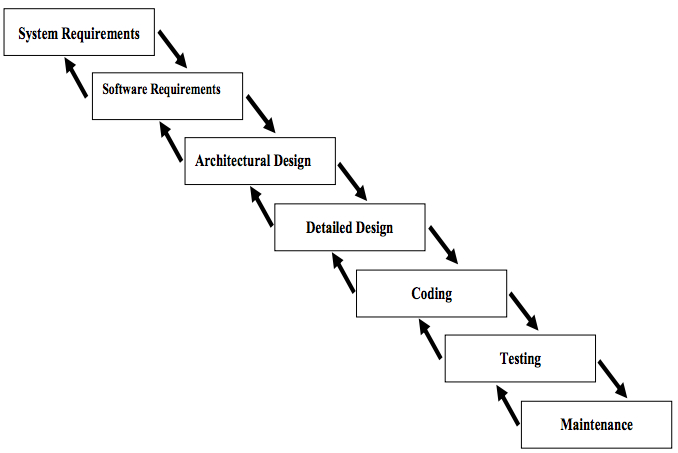
\includegraphics[scale=0.7]{Picture/waterfall.jpg}
\caption{Waterfall model}
\label{fig:waterfall} % 
\end{figure}

\section {Scrum}
\label{sec:Scrum}
"Scrum is the best-known of the Agile frameworks. It is the source of much of the thinking behind the values and principles of the Agile Manifesto". These values are:

\begin{center}
\textbf{Individuals and interactions}  \textit{over processes and tools} \\
\textbf{Working software} \textit{over comprehensive documentation} \\
\textbf{Customer collaboration} \textit{over contract negotiation} \\
\textbf{Responding to change} \textit{over following a plan} \\
\parencite{Scrum}.
\end{center}
%"Individuals and interactions over processes and tools", "Working software over comprehensive documentation", "Customer collaboration over contract negotiation" and "Responding to change over following a plan" from the Agile Manifesto\parencite{Scrum}. 

These principles of Scrum and Agile manifesto are not so rigid as the principles of the Waterfall method. Some may say that Scrum is the opposite of the Waterfall method \parencite{cocco2011simulating}. 

Scrum have three main roles, the Product Owner, the Scrum Master and the members of the development team. The Product owner in collaboration with the Scrum Master decides which work to be prioritized in the backlog. The backlog represents the tasks to be done in order to complete the project. The Scrum Master acts like a team leader and helps the development team and the organization to take best advantages of Scrum. The development team works on tasks specific for current sprint \parencite{Scrum}.

Sprint is a time-boxed interval over a given time. The Scrum framework suggests duration of sprints to be from one to four weeks. Before each sprint, a sprint planning meeting is conducted with all the team members attending.  A Sprint planning meeting is held so the team can discuss tasks from the backlog and come to an agreement of which tasks to be put in the minimal backlog \parencite{Scrum}.

In each sprint a minimal backlog is created so the developer knows which tasks to work on in the current sprint. The Product Owner and the team members discuss and decide which tasks from the backlog to be added to the minimal backlog. After the minimal backlog is complete, the Product Owner and the team members discuss each task in order to get a better and shared understanding of what is required to complete the tasks \parencite{Scrum}. 

One of the main principles in Scrum is that it requires that at least one new feature is ready for release after each sprint. The feature should be a visible part of the product in order to get feedback from end-users. So all the tasks in the minimal backlog combined should be a visible part of the product \parencite{Scrum}.


\section {Lean}
\label{sec:Lean}
"Lean is all about getting the right things to the right place at the right time the first time while minimizing waste and being open to change" \parencite{741480}.
The Lean approach was introduced around 1948 in manufacturing in Japan.  In 1975, Toyota was able to create almost 50 more production units per employee than in 1948 due to the Lean approach \parencite{manning}. Lean strives to maximize the value produced by an organization and delivered to costumer. This is done by finding and eliminate waste, controlling variability and maximizing the flow of delivered software all within the culture of continuous improvements \parencite{DavidAnderson}. In 2003 Mary and Tom Poppendieck first introduced Lean thinking to software development. Poppendieck published the book "Lean Software Development: An Agile Toolkit" \parencite{Lean:2003}. In the book, Poppendieck stated that an important tool to manage work flow is the concept of pull-systems, which means tasks are put in production only when a costumer asks for it \parencite{Lean:2009}.
The pull based method Kanban has in recent years been introduced more and more to software development, and is becoming one of the keys to Lean practice in software development \parencite{DavidAnderson}. In Lean there are eight fundamental principles \parencite{poppendieck2003lean}.
\begin{enumerate}
\item \textbf{Start Early:}  Do not wait for details. As soon as enough information is gathered start the development activity. Get everyone involved in figuring out the details. Do not build any walls between people, make people collaborate and start a two-way communication as soon possible. This will start the learning cycle as well.

\item \textbf{Learn Constantly:} Start with a breadth-first approach, explore multiple options. The system is expected to change, so focus on creating simplicity code and robustness so the system is easy to change

\item \textbf{Delay Commitment:} 
In order to delay commitment, automated testing and refactoring are essential for keeping code changeable. 

\item \textbf{Deliver Fast:}
Deliver fast mark of excellent operational capability. The whole idea of \textbf{delaying commitment} is to make every decision as late as possible when one have the most knowledge.
\item \textbf{Eliminate Waste:}
The only thing worth doing is deliver value to the costumer, anything else is waste.  Discover waste and eliminate it is the first key of Lean.  Lean suggests using a value stream map for removing waste. A Value Stream Map (VSM) is a map over the whole company chain. VSM helps visualize where waste is located within the company.
\item \textbf{Empower the team:} When one is going to deliver fast, there is no room for central control. The work environment should be structured so work and workers are self-directing.

\item \textbf{Build Integrity In:} Lean software is build with integrity. That's why one of the principles in Lean suggests that tests are integrated into software development just as any code, so it becomes a part of the delivered product. 

\item \textbf{Avoid Sub-optimization:} In software development it is normal to break down a complex problem into small parts of the problem in order to minimize the complexity.  If some of the parts are sub-optimized, bottlenecks can occur. For example, if ten developers are hired to work on tasks, but only three testers are hired. The development process is sub-optimized since the developers will likely produce more than the tester can test and that could cause bottleneck.
\end{enumerate}


\section{Kanban}
\label{sec:Kan}
\iffalse
Shinkle defined novice and more experience kanban-users with a descriptive analogy \parencite{Shinkle}:
''Think about a typical person wanting to bake a cake. They go to the store, purchase a boxed cake mix, and follow the directions as described on the back of the box. They have little to no knowledge about how to alter the recipe nor do they have a desire to do so. Their goal is simply to bake a cake.''

''An advanced beginner understands how to apply some context to the instructions or rules on the back of the box. They can make minor adjustments for things like altitude, pan size, oven conditions, etc. They are still following the basic recipe, but can make minor adjustments likely based on previous experiences." According to Shinkle, principles like WIP-limit will be adopted when the user has some experience with Kanban. 
\fi


Toyota production system introduced Kanban as a scheduling system for Lean and just-in-time (JIT) production during late 1940's and in the early 1950's in order to catch up with the American car industry. The Kanban method combined with the Lean approach was a success for Toyota. The success was noticed by the software development industry among others \parencite{Conboy}, \parencite{ono1988toyota}. In the recent years, the software industry has seen an increasing amount of project that applies Kanban and Lean principles \parencite{DavidAnderson}, and this is one of the reasons why this work will focus on Kanban, more specific, one of its key principles WIP-limits.

''One can define Kanban software process as a WIP-limited pull system visualized by the Kanban board''  \parencite{DavidAnderson}.
One of the most important people in Kanban software development, David Anderson  also referred to as ''father of Kanban in the software development industry''  \parencite{InfoQ:2013:May:Online} and author of the book "Kanban: Successful Evolutionary Change for Your Technology Business"\parencite{0984521402} stated ''If you think that there was Capability Maturity Model Integration, there was Rational Unified Process, there was Extreme Programming and there was Scrum, Kanban is the next thing in that succession.''   \parencite{InfoQ} .

In software development, Kanban splits the major problem into many small pieces of problems. When the small pieces are defined by the team, the problems are put up on the Kanban board to visualize the problems, track what others are working on and see potential bottlenecks during development. Shinkle stated that when people start to understand Kanban, they easily discover where the bottlenecks are \parencite{Shinkle}. In short, Kanban systems focus on \parencite{DavidAnderson}:

\begin{itemize}
\item continuous flow of work,
\item	no fixed iterations or sprints,
\item work is delivered when it is done,
\item teams only work on few tasks at the time specified by the WIP-limit and
\item make constant flow of released tasks.
\end{itemize}


Contrary to Scrum, Kanban do not use the principles of sprints or estimations. In Kanban the tasks do not need to be estimated or finished within a certain time. In the paper "Simulation of software maintenance process, with and without a work-in-process limit" \parencite{SMR:SMR1599} the authors found out that if they let the developers work with small tasks and are not interrupted, they will be more effective. They also found out that Scrum was too rigid for the development team because when the team had to estimate tasks, they felt interrupted.  The estimation and sprint meetings worked counterproductive in their case. The authors made the developers change to Lean-Kanban.  The change implied the removal of sprints and estimation. After removing sprints and estimation the teams increased the ability to perform work, lower the lead time and meet the production dates \parencite{SMR:SMR1599}.

In the papers"Quantifying the Effect of Using Kanban versus Scrum:" the company also felt that the Scrum approach was too rigid. The paper also reported positive results when the team changed to Kanban.  The company almost halved its lead time, reduced the number of weighted bugs by 10 percent, and improved productivity \parencite{Dag}. Other papers also state that Scrum maybe too rigid and that's Kanbans advantages over Scrum \parencite{beedle1999scrum} \parencite{brekkanintroducing} .  

\subsection {Kanban Board}
''The Kanban board makes it clear to all the team members the exact status of progress, blockages, bottlenecks and they also signal possible future issues to prepare for''\parencite{Joyce}.  The Kanban board is one of many tools in Kanban. it is used to control WIP, increase the information flow with visualization \parencite{SMR:SMR1599}. A Kanban board is illustrated in Figure \ref{kanban_board}. Each column in Figure has \ref{kanban_board} an intuitive name in order to describe itself so the developers easily can track where each task is. 

The columns are named "Backlog", "In progress" and "Done".  Each column can have a WIP-limit to specify how many items in progress there are allowed in the column \parencite{Joyce}. In Figure \ref{kanban_board} the WIP-limit is stated under the column name. The backlog column has a WIP-limit of 4, In progress has 5 and Done doesn't need a WIP-limit. 

The yellow stickers represent the tasks. Some development teams follow the path to mark stickers with different colors representing the severities or by marking if its a feature or a bug. In the paper "Kanban Implementation in a Telecom Product Maintenance" for instance, the stickers has three different colors, green, yellow and red depending on how close to overdue the tasks are. If the sticker is red, the task is already overdue, if the tasks are soon-to-overdue its marked with yellow stickers \parencite{6068363}. In another project, they used yellow sticky notes for scenarios, blue for bugs, pink for issues \parencite{Shinkle}.
\begin{figure}[!htbp]
\centering
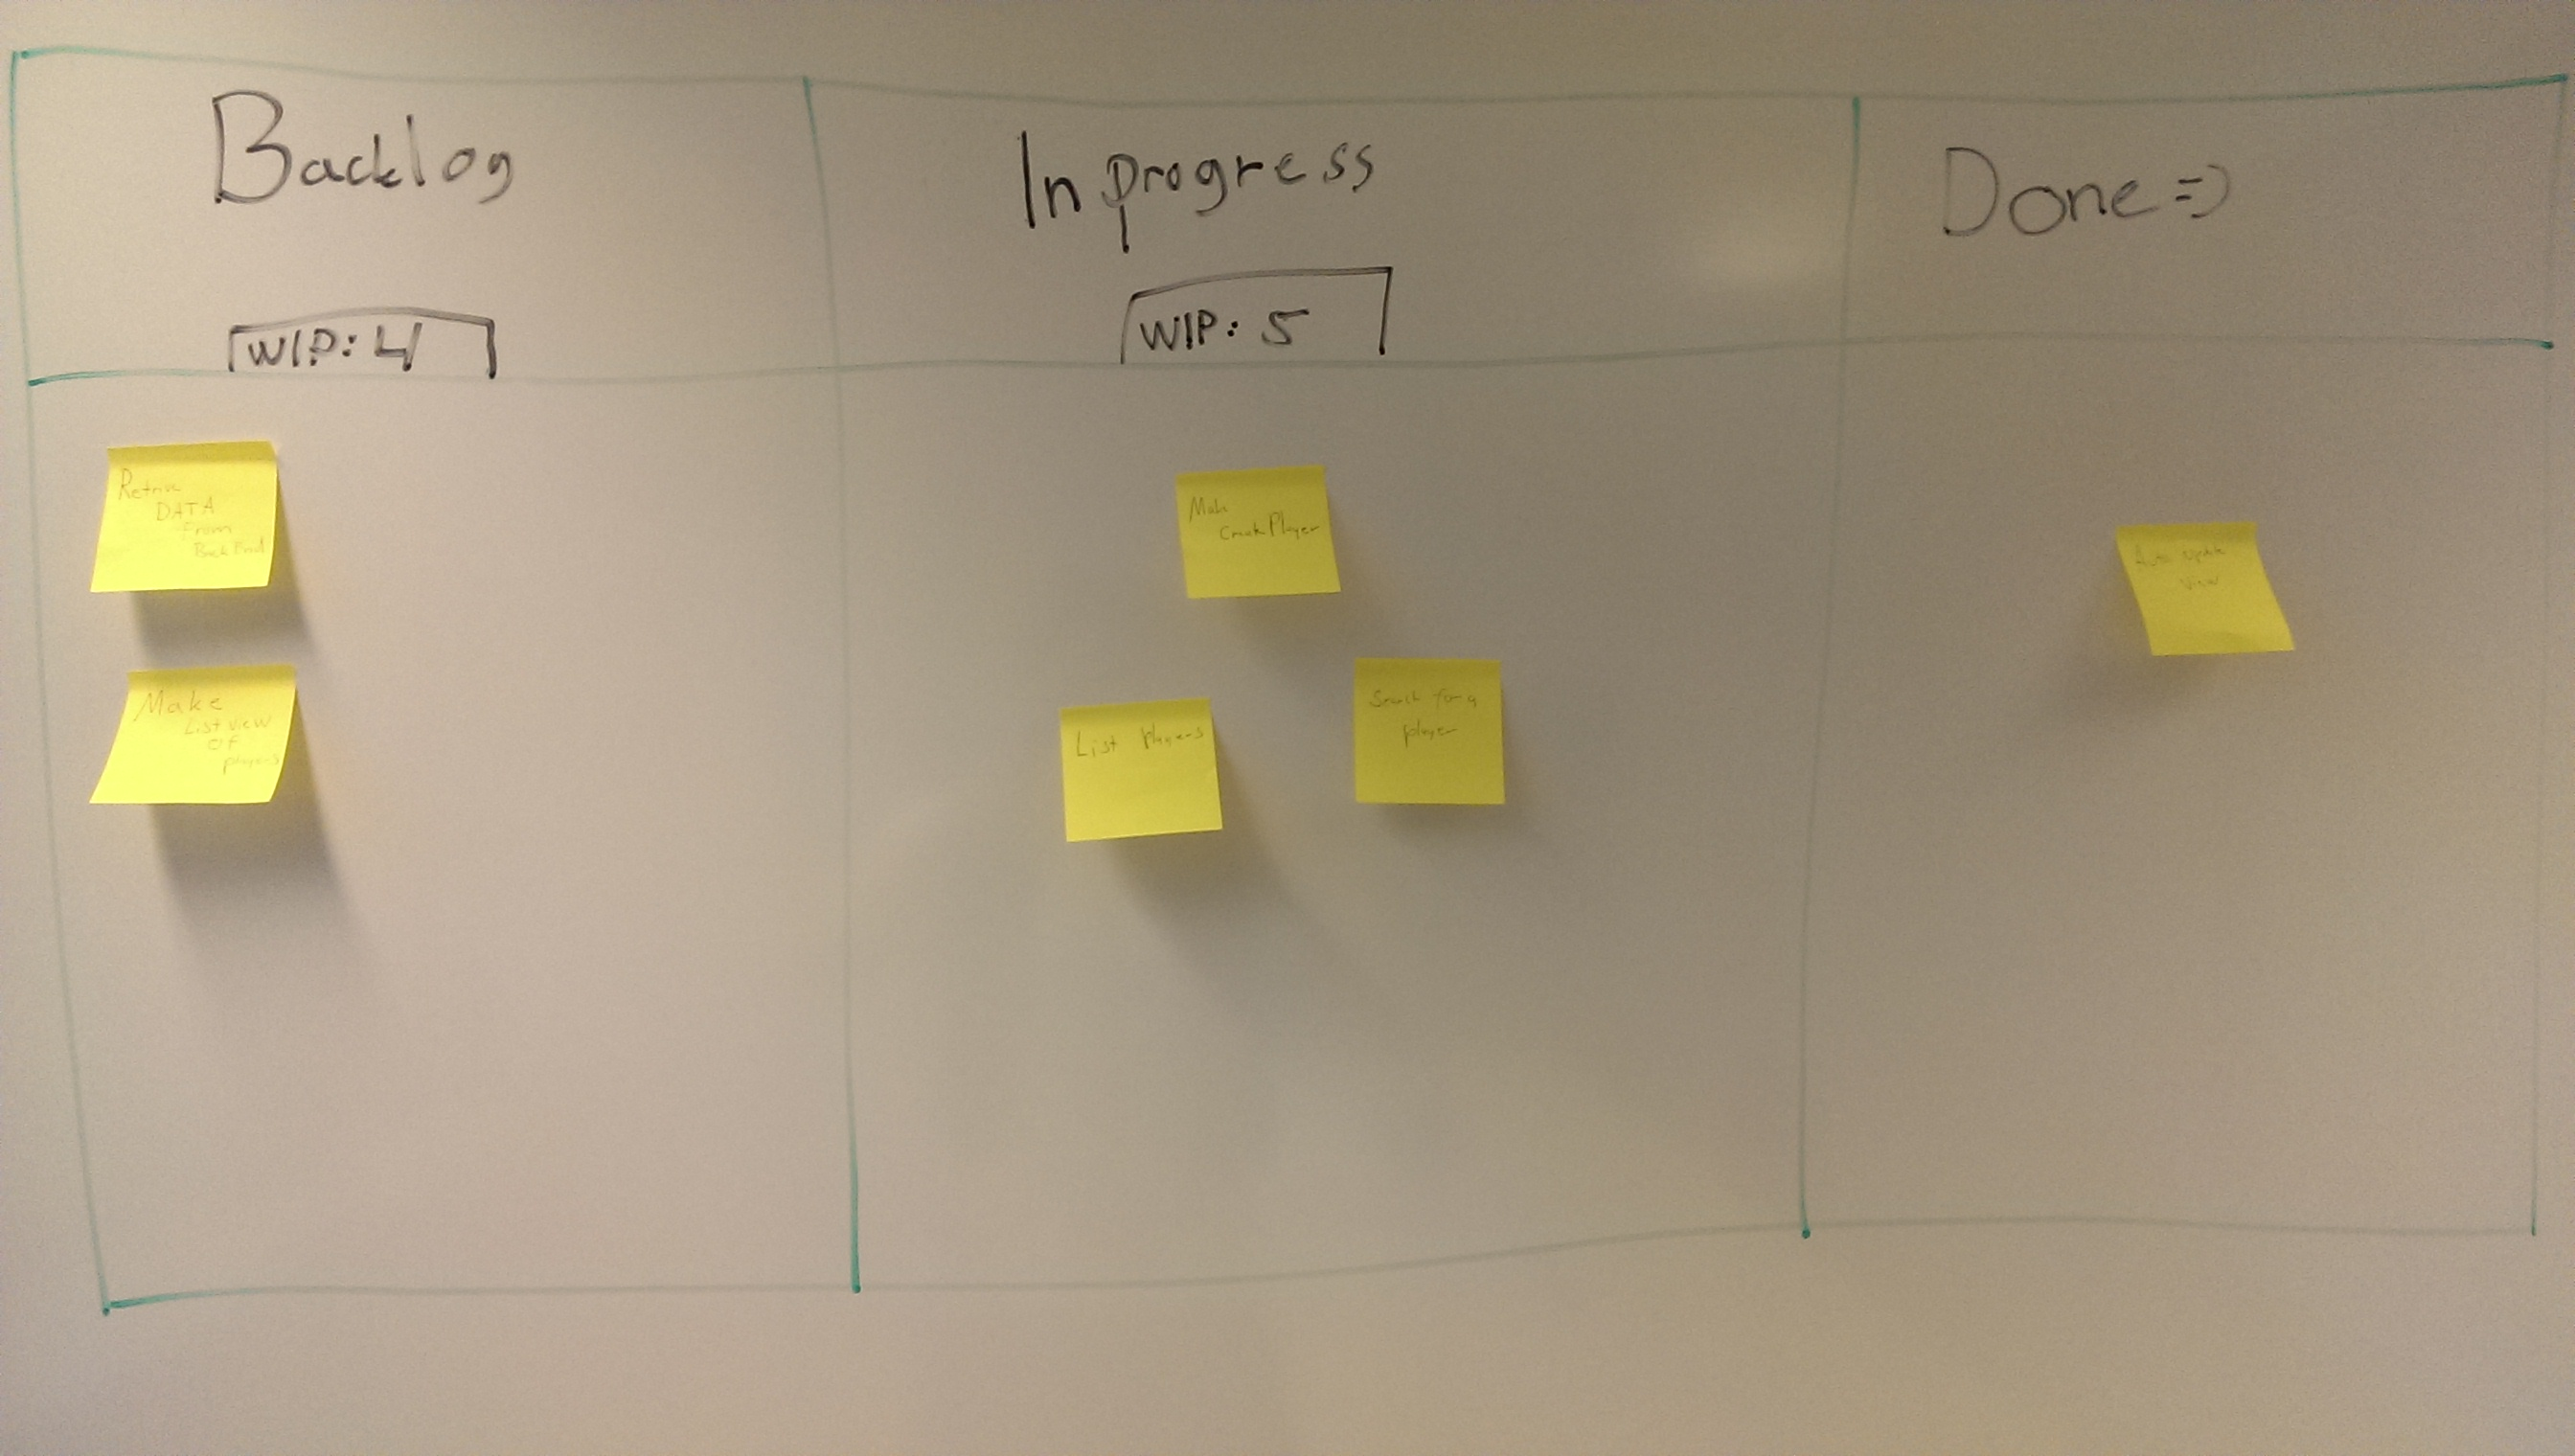
\includegraphics[width=\textwidth]{Picture/kanban_board.jpg}
\caption{Example of a Kanban board}
\label{kanban_board}
\end{figure}

\subsection{WIP-limit}
\label{WIPsec}
''WIP-limits seem to be the worst understood part of the Kanban system. When used properly, it exposes bottlenecks and reduces lead time for individual work items. Used improperly, it can starve developers for work or result in too many people working on the same work items.'' \parencite{Shinkle}

WIP-limit is one of the core principles in Kanban \parencite{6068363}. WIP-limit helps to reduce overhead by limit task-switching for each developer and make constant flow of tasks throughout the development \parencite{DavidAnderson}. One way to explain WIP and the asserted impact of WIP-limit is to use cars and roads as analogy. All roads have a maximum capacity of cars. When this limit is reached, traffic jam occurs and the throughput of cars decreases and lead time increases. The same can be said about software development teams. A software team has a maximum number of tasks they can perform, if the team is pushed over the maximum limit, the throughput of tasks may decreases and lead time may increases.

When first implementing Kanban, Shinkle explains that the users often do not care about WIP or setting a WIP-limit, but rather the visibility of Kanban through the Kanban board. When users gain more experience with Kanban, they start to attempt the principles of WIP-limit \parencite{Shinkle}. Srinivasan, Ebbing and Swearing said that setting the WIP-limit is not easy. They suggest that the WIP-limit is set, and then observe throughput, and adjust after that \parencite{Mandyam}. In the book "Kanban and Scrum - making the most of both" suggests Kniberg that you start by limiting WIP, then experiment with it \parencite{Kniberg}. The paper "Lean Software Management" \parencite{Kniberg} and the "Impact of Kanban on Software Project Work" \parencite{Ikonen} both suggest that WIP should be minimized as well. The conclusion of the studies are to keep the WIP-limit low and experiment by slowly increase the WIP-limit until the throughput decreased and lead time increased, then you know that the previous WIP-limit was the perfect one.

The Section \ref{sub:wip:vs:wip} shows a summary of the the papers by Giulio Concas, Hongyu Zhang \parencite{SMR:SMR1599}  and David Anderson, Giulio Concas, Maria Ilaria Lunesu, and Michele Marchesi \parencite{DavidAnderson}. The papers researched the difference between WIP-limit and unlimited WIP. Section \ref{sub:sub:benefits} shows the importance of WIP-limit, stated by various researches. 

On "how to determine WIP-limit", one paper was found. If one implements Kanban with sprints or uses Scrum, \L ukasz proposes to use the effectiveness metric to help determine the WIP-limit.The effectiveness metric shown in formula \ref{WIPEQ}, should be applied after end sprint according to \L ukasz. After each sprint, one can apply the effectiveness metric and the result could be used as a guideline for WIP-limit for the next sprint. The effectiveness metric takes the number of bugs found \textit{(ai)} and the number of bugs found by external people (e.g. lawyers, accountants, coaches, consultants, translators, internal and external service providers etc.) \textit{(ei)}, and minus \textit{ai} and \textit{ei}, then divide the result by \textit{ai} and multiply it by 100\%  as shown in formula \ref{WIPEQ} \parencite{Sienkiewicz}

\begin{equation} \label{WIPEQ}
Ei=\frac{(ai-ei)}{ai}*100\%
\end{equation}

\subsubsection {WIP-limit vs. Unlimited WIP}
\label{sub:wip:vs:wip}
In an paper cite by Giulio Concas and Hongyu Zhang \parencite{SMR:SMR1599}, they simulated two different software maintenance processes. The first process was based on 4 years of experience with Microsoft maintenance team. The second process was from a Chinese software firm.  The simulation executed 10 runs and one of the results were the average of closed tasks was 4145 when the WIP was limited and 3853 when the limit was not limited (about 7\% less). The paper concludes findings as; developers are more focused on fixing few issues, because the number of issues they can work on is limited. The developers are more likely to continue on the issue from the day before, rather than starting on another issue. This reduces overhead, because when developers start on a new issue, they need time to familiarize themselves with the code and the issue. That could create unnecessary overhead if some developer already has done it, but that developer is now working on another issue. 

The study also showed that WIP-limit could improve throughput and work efficiency, because WIP-limits prevents task switching. The paper also did a simulation of a process who was originally without WIP-limits, with WIP-limits. The study showed the simulated process with WIP-limits out performed the original process. \parencite{SMR:SMR1599}.

The paper by David Anderson et al. \parencite{DavidAnderson} did a simulation of lean-kanban approach with the impact of WIP-limit vs. no WIP-limit on developers with skills in different activities. The four skill activities from the paper were design, development, testing and deployment. 

The paper did four different simulations.  A simulation with WIP-limits and seven developers with skill in two of the four activities. A simulation with no WIP-limit and seven developers with skilled in two of the four activities. A simulation with WIP-limits and seven developers with skill in all of the activities. A simulation with no WIP-limits and seven developers with skill in two of the four activities.

The paper concluded that the last two is unlikely in the real world, because there is rarely a whole team with developers skilled in all activities. 
When the developers had skill in two out of four activities, the WIP-limit simulation used 100 days, but the non WIP-limit simulation used 120 days. The simulation with WIP-limit showed an almost constant flow of features that completed, while in the same simulation with no WIP-limit, the flow of features was much more irregular \parencite{DavidAnderson}.

\subsubsection{Benefits with setting WIP-limit}
\label{sub:sub:benefits}
This subsection contains excerpt from papers from various authors that have done study on WIP-limit. 

\begin{enumerate}
\item Lowering the WIP-limit will help people avoid task switching. When switching tasks, it is more difficult to be able to fully concentrate. \parencite{Ikonen}.
\item There's stated when using short-cycle times and Kanban board to WIP-limit, the software development team's learning is increased \parencite{Joyce}:
\item WIP-limit increases productivity \parencite{Joyce}.
\item WIP-limit reduce cycle time \parencite{Ola}
\item When WIP was too high, lead times grew and as a result so did the bugs and rework \parencite{Shinkle}.
\vspace{-0.3em}
\item  WIP-limits are important to reduce lead times \parencite{KanbanWay} 
\end{enumerate}

Both the studies on WIP-limit vs. no limit and the papers shows the importance of WIP-limit. If  \L ukasz's effectiveness equation \ref{WIPEQ} is regarded , there is no clear rule on how to determine WIP-limit even though WIP is supposed to be a crucial principle in order to take full advantage of Kanban.

\section {Lead time}
\label{sec:in:lt}
''Lead time is the total elapsed time from when a customer requests software to when the finished software is released to the customer'' \parencite{Joyce}. Lead time is measured to track how quickly software is delivered to customers \parencite{Joyce}. Lead time could be an essential ingredient when you look for the optimal WIP, if there is one.  Often in a project, lead time is split into pieces, so every task has its own lead time. This gives the development teams the advantages to experiment with different WIPs in order to see the different lead times, then measure which WIP that suits this project the best. 

According to the paper "Quantifying the effect of Using Kanban versus Scrum" \parencite{Dag} the citation by Middleton and Joyce above is close to definition of what lead time is. They define lead time as the amount of time that passed from the moment that the development team receives a request to the moment that it completes the work item. The reason why the paper disapproves the definition by Middleton and Joyce is because: "The amount of time a work item remains in the backlog queue before it is put on the board is a function of priority, not whether the company uses Scrum, Kanban or other development methods. Furthermore, companies that develop and sell products to many customers might propose new features themselves and put them on the backlog before any customers request them. Second, given a policy of two or three releases a year, the result of a work item isn't delivered to the customer immediately after it is finished'' \parencite{Dag}.



\section{Just-In-Time}
"Just-In-Time is based on delivering only the necessary products, to the necessary time and the necessary quantity" \parencite{JIT}.
Just-In-Time (JIT) was introduced in the 1970s by Toyota in combination with Lean \parencite{javadian2013just}.  JIT has been introduced to increase productivity through waste reduction and increasing the value added in the production processes. To explain the JIT principle, Mary and Tom Poppendieck use the picture shown in Figure \ref{JITE}  \parencite{JIT} \parencite{Lean:2006}. The stream reflects the inventory.  Under the stream, there are rocks located in different sizes. The rocks illustrates waste and problems that can occur.  If the stream level is lowered, the rocks are more visualized. At this point you have to clear out rocks (remove waste and problems) in order to make the boat continue it is journey, or it will crash into the rocks. After the rocks are cleaned out, one can lower the stream level again and continue the procedure until there are only pebbles left. Then the boat can float without problems.

If one lower the stream (inventory), problems and waste will become visible (visualized by rocks). Lean wants to lower inventory in order to make problems and waste occur, because when problems and waste occurs, you are able to fix the problems and remove the waste. Fixing the problem and removing the waste has several benefits such as, your process could be optimized and you are one step closer to have zero problems and zero waste.  \parencite{JIT} \parencite{Lean:2006}.

In Software development the JIT principle means one should not deliver anything before its demanded. For example, a development team adds two new features to a product without the stakeholders asking for it and it turns out the stakeholders do not want it. Then the team has produced waste. 
\begin{figure}[ht!]
\centering
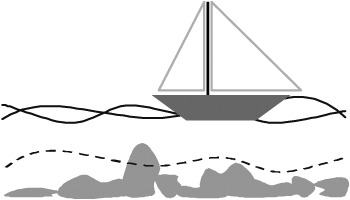
\includegraphics[width=90mm]{Picture/JIT.jpg}
\caption{JIT example}
\label{JITE} % JIT example
\end{figure}

\section{Throughput}
''The output of a production process (machine, workstation, line plant) per unit time (e.g., parts per hour) is defined as the systems throughput or sometimes throughput rate'' \parencite{Adams}.
The main concept of throughput is to measure how productive teams, people or companies are. Throughput is measured in number of finished delivered tasks or units per hour, day, week, month, quarter or year. A key factor in successfully measuring throughput in software development is to specify a standard size for each task. If the standard is not specified there is little use in throughput measurements.  \parencite{Throughput}. To illustrate throughput with different task sizes an example is provided:  

Lets say Team x had a throughput of eighteen tasks after the first quarter, twenty after the second, fifteen after the third and twelve after the last quarter. Team x used Scrum the first two quarters and Kanban the last two as illustrated in table \ref{tt}. It will look like team x benefits most from Scrum. But if the task during the Kanban time was twice the size of Scrum, Kanban would suite team x the best. So, to get valid result from throughput measurements, the size of tasks has to be agreed upon by the teams or company.
\begin{table}[ht]
\begin{center}
    \begin{tabular}{| l | l | l | l |}
    \hline
    Quarter & Throughput & Method\\ \hline
    1 & 18 & Scrum\\ \hline
    2 & 20 & Scrum \\ \hline
    3 & 15 & Kanban\\ \hline
    4 & 12 & Kanban\\ \hline
    \end{tabular}
\caption{Throughput}
\label{tt} %% throughput table
\end{center}
\end{table}

\section{Code churn}
\label{sec:Churn}
"Churn is defined as the sum of the number of lines added, deleted, and modified in the source code" \parencite{Dag}.
Churn is a measure that is not as familiar as lead time, throughput or WIP in the software industry. Churn is a term used as surrogates for effort in software engineering. Many studies in software engineering use code churn or revisions as surrogate measure of effort \parencite{yamashita2012quantifying}. Emam stated that "analysts should be discouraged from using surrogate measures, such as code churn, unless there is evidence that they are indeed good surrogates" \parencite{el2000methodology}. The study by Sj\o berg et al. showed that churn could be used as a surrogate for tasks size \parencite{yamashita2012quantifying}. 


\section{Software Innovation}
\label{sec:SI}
Software Innovation\footnote{http://www.software-innovation.com/} is a Scandinavian software company. SI develops and delivers Enterprise Content Management applications that helps organizations improve and increase efficiency in document management, case handling and technical document control. SI builds products around the Microsoft Sharepoint platform. \parencite{Dag}, \parencite{SI}.

SI has approximately 300 employees in Oslo, Copenhagen, Stockholm and Bangalore \parencite{SI}. From 2001 to 2006, SI used the Waterfall process. In 2007, SI changed to Scrum, and in 2010, SI went from Scrum to Kanban \parencite{Dag}.
\newpage
Table \ref{table:teams} shows the size of the ten teams vs. quarter. The team size is used as a variable to compute the result for work. Team seven, shown in Table \ref{Team:7} contribute data from 2010 to 2012. After 2012, team seven was shut down.

\begin{figure}[h]
\begin{subfigure}[b]{.2\textwidth}
\center
 \scalebox{0.40}{
\begin{tabular}{ | l | r | r | }
\hline
 \bf{Year} & \bf{Quarter} & \bf{Team Size} \\ \hline
2010 & 3 & 6 \\ \hline
	2010 & 4 & 3 \\ \hline
	2011 & 1 & 16 \\ \hline
	2011 & 2 & 28 \\ \hline
	2011 & 3 & 2 \\ \hline
	2011 & 4 & 38 \\ \hline
	2012 & 1 & 35 \\ \hline
	2012 & 2 & 34 \\ \hline
	2012 & 3 & 32 \\ \hline
	2012 & 4 & 29 \\ \hline
	2013 & 1 & 24 \\ \hline
	2013 & 2 & 37 \\ \hline
	2013 & 3 & 23 \\ \hline
	2013 & 4 & 23 \\ \hline
	Total & & 330  \\ \hline
\end{tabular}
}
\caption{Team size - team one}
 \label{Team:1}
\end{subfigure}
\begin{subfigure}[b]{.2\textwidth}
\center
 \scalebox{0.40}{
\begin{tabular}{ | l | r | r | }
\hline
 \bf{Year} & \bf{Quarter} & \bf{Team Size} \\ \hline
	2010 & 3 & 10 \\ \hline
	2010 & 4 & 15 \\ \hline
	2011 & 1 & 13 \\ \hline
	2011 & 2 & 12 \\ \hline
	2011 & 3 & 15 \\ \hline
	2011 & 4 & 14 \\ \hline
	2012 & 1 & 15 \\ \hline
	2012 & 2 & 7 \\ \hline
	2012 & 3 & 8 \\ \hline
	2012 & 4 & 9 \\ \hline
	2013 & 1 & 10 \\ \hline
	2013 & 2 & 7 \\ \hline
	2013 & 3 & 7 \\ \hline
	2013 & 4 & 8 \\ \hline
	Total & & 150  \\ \hline
\end{tabular}
}
\caption{Team size - team two}
 \label{Team:2}
\end{subfigure}
\begin{subfigure}[b]{0.2\textwidth}
\center
 \scalebox{0.40}{
\begin{tabular}{ | l | r | r | }
\hline
 \bf{Year} & \bf{Quarter} & \bf{Team Size} \\ \hline
2010 & 3 & 6 \\ \hline
	2010 & 4 & 9 \\ \hline
	2011 & 1 & 7 \\ \hline
	2011 & 2 & 10 \\ \hline
	2011 & 3 & 9 \\ \hline
	2011 & 4 & 10 \\ \hline
	2012 & 1 & 11 \\ \hline
	2012 & 2 & 11 \\ \hline
	2012 & 3 & 13 \\ \hline
	2012 & 4 & 13 \\ \hline
	2013 & 1 & 13 \\ \hline
	2013 & 2 & 7 \\ \hline
	2013 & 3 & 8 \\ \hline
	2013 & 4 & 8 \\ \hline
	Total & &135  \\ \hline
\end{tabular}
}
\caption{Team size - team three}
 \label{Team:3}
\end{subfigure}
\begin{subfigure}[b]{0.2\textwidth}
\center
 \scalebox{0.40}{
\begin{tabular}{ | l | r | r | }
\hline
 \bf{Year} & \bf{Quarter} & \bf{Team Size} \\ \hline
	2010 & 3 & 3 \\ \hline
	2010 & 4 & 8 \\ \hline
	2011 & 1 & 4 \\ \hline
	2011 & 2 & 4 \\ \hline
	2011 & 3 & 4 \\ \hline
	2011 & 4 & 4 \\ \hline
	2012 & 1 & 4 \\ \hline
	2012 & 2 & 2 \\ \hline
	2012 & 3 & 3 \\ \hline
	2012 & 4 & 5 \\ \hline
	2013 & 1 & 7 \\ \hline
	2013 & 2 & 5 \\ \hline
	2013 & 3 & 5 \\ \hline
	2013 & 4 & 5 \\ \hline
	Total & &63  \\ \hline
\end{tabular}
}
\caption{Team size - team four}
 \label{Team:4}
\end{subfigure}
%%%%%%% DEL TO TEAM 5-8
\begin{subfigure}[b]{0.1\textwidth}
\center
 \scalebox{0.40}{
\begin{tabular}{ | l | r | r | }
\hline
 \bf{Year} & \bf{Quarter} & \bf{Team Size} \\ \hline
	2010 & 3 & 5  \\ \hline
	2010 & 4 & 13  \\ \hline
	2011 & 1 & 14  \\ \hline
	2011 & 2 & 25  \\ \hline
	2011 & 3 & 21   \\ \hline
	2011 & 4 & 23   \\ \hline
	2012 & 1 & 25   \\ \hline
	2012 & 2 & 19   \\ \hline
	2012 & 3 & 24   \\ \hline
	2012 & 4 & 18   \\ \hline
	2013 & 1 & 31   \\ \hline
	2013 & 2 & 29   \\ \hline
	2013 & 3 & 27   \\ \hline
	2013 & 4 & 11   \\ \hline
	Total & &285  \\ \hline
\end{tabular}
}
\caption{Team size - five}
 \label{Team:5}
\end{subfigure}

\begin{subfigure}[b]{0.3\textwidth}
\center
 \scalebox{0.40}{
\begin{tabular}{ | l | r | r | }
\hline
 \bf{Year} & \bf{Quarter} & \bf{Team Size} \\ \hline
	2010 & 3 & 5  \\ \hline
	2010 & 4 & 6  \\ \hline
	2011 & 1 & 6  \\ \hline
	2011 & 2 & 6  \\ \hline
	2011 & 3 & 5   \\ \hline
	2011 & 4 & 5   \\ \hline
	2012 & 1 & 4   \\ \hline
	2012 & 2 & 6   \\ \hline
	2012 & 3 & 6   \\ \hline
	2012 & 4 & 9   \\ \hline
	2013 & 1 & 9   \\ \hline
	2013 & 2 & 9   \\ \hline
	2013 & 3 & 9   \\ \hline
	2013 & 4 & 14   \\ \hline
Total & &99  \\ \hline
\end{tabular}
}
\caption{Team size - team six}
 \label{Team:6}
\end{subfigure}
\begin{subfigure}[b]{0.3\textwidth}
\center
 \scalebox{0.40}{
\begin{tabular}{ | l | r | r | }
\hline
 \bf{Year} & \bf{Quarter} & \bf{Team Size} \\ \hline
 	2010 & 3 & 10  \\ \hline
	2010 & 4 & 8   \\ \hline
	2011 & 1 & 8   \\ \hline
	2011 & 2 & 6   \\ \hline
	2011 & 3 & 8   \\ \hline
	2011 & 4 & 9   \\ \hline
	2012 & 1 & 10   \\ \hline
	2012 & 2 & 5   \\ \hline
	2012 & 3 & 9   \\ \hline
	2012 & 4 & 3   \\ \hline
	Total & &76  \\ \hline
\end{tabular}
}
\caption{Team size - team seven}
 \label{Team:7}
\end{subfigure}
\begin{subfigure}[b]{0.3\textwidth}
\center
 \scalebox{0.40}{
\begin{tabular}{ | l | r | r | }
\hline
 \bf{Year} & \bf{Quarter} & \bf{Team Size} \\ \hline
 	2010 & 4 & 2 \\ \hline
	2011 & 1 & 8 \\ \hline
	2011 & 2 & 8 \\ \hline
	2011 & 3 & 13 \\ \hline
	2011 & 4 & 9 \\ \hline
	2012 & 1 & 10 \\ \hline
	2012 & 2 & 2 \\ \hline
	2012 & 3 & 25 \\ \hline
	2012 & 4 & 11 \\ \hline
	2013 & 1 & 22 \\ \hline
	2013 & 2 & 21 \\ \hline
	2013 & 3 & 23 \\ \hline
	2013 & 4 & 8 \\ \hline
	Total & &162  \\ \hline
\end{tabular}
}
\caption{Team size - team eight}
 \label{Team:8}
\end{subfigure}




%%%%%% DEL tree TEAM 9-10
\begin{subfigure}[b]{0.5\textwidth}
\center
 \scalebox{0.40}{
\begin{tabular}{ | l | r | r | }
\hline
 \bf{Year} & \bf{Quarter} & \bf{Team Size} \\ \hline
 	2010 & 4 & 5 \\ \hline
	2011 & 1 & 8 \\ \hline
	2011 & 2 & 7 \\ \hline
	2011 & 3 & 7 \\ \hline
	2011 & 4 & 9 \\ \hline
	2012 & 1 & 10 \\ \hline
	2012 & 2 & 8 \\ \hline
	2012 & 3 & 10 \\ \hline
	2012 & 4 & 12 \\ \hline
	2013 & 1 & 8 \\ \hline
	2013 & 2 & 9 \\ \hline
	2013 & 3 & 8 \\ \hline
	2013 & 4 & 8 \\ \hline
	Total & &109  \\ \hline
\end{tabular}
}
\caption{Team size - team nine}
 \label{Team:9}
\end{subfigure}
\begin{subfigure}[b]{0.5\textwidth}
\center
 \scalebox{0.40}{
\begin{tabular}{ | l | r | r | }
\hline
	 \bf{Year} & \bf{Quarter} & \bf{Team Size} \\ \hline
	2010 & 3 & 3 \\ \hline
	2010 & 4 & 11 \\ \hline
	 2011 & 1 & 12 \\ \hline
	 2011 & 2 & 9 \\ \hline
	2011 & 3 & 4 \\ \hline
	 2011 & 4 & 17 \\ \hline
	2012 & 1 & 20 \\ \hline
	2012 & 2 & 17 \\ \hline
	2012 & 3 & 18 \\ \hline
	2012 & 4 & 13 \\ \hline
	2013 & 1 & 17 \\ \hline
	2013 & 2 & 9 \\ \hline
	2013 & 3 & 10 \\ \hline
	2013 & 4 & 10 \\ \hline
	Total & &170  \\ \hline
\end{tabular}
}
\caption{Team size - team ten}
 \label{Team:10}
\end{subfigure}
\caption[Optional caption for list of figures]{Caption of team size for teams in SI}
\label{table:teams}
\end{figure}




\chapter{Research Methods}
\label{chap:RM}
In this chapter the research methods used in this work will be introduced and the reason why the data set from Software Innovation was chosen. Section \ref{sec:CS} gives a brief introduction to the research method "Case Study".  Section \ref{sec:coc} is about the choice of case and complementary information about Software Innovation. 


\section{Case study}
\label{sec:CS}
To answer the research questions, a case study was conducted.  A case study is used to explore causation in order to find underlying principles \parencite{0078285763}\parencite{9781412960991}.  But which methods one can use in a case study or how the case study is conducted is ambiguous.  It might be that the case study is qualitative or quantitate.  A case study might utilize a particular type of evidence (for example ethnographic, participant observation or field research).  Jennifer Platt stated: "Much case study theorizing has been conceptually confused because too many different themes have been packed into the idea "case study" \parencite{0521676568}.  John Gerring stated: "A case study may be understood as the intensive study of a single case where the purpose of that study is -- at least in part to shed light on a larger class of cases  \parencite{0521676568}. As one can see, there is no clear rule of how to conduct a case study or what it is. 


%John also stated: "Case connotes a spatially delimited phenomenon (a unit) observed at a single point in time or over a period of time"\parencite{0521676568}. 
In this work, the case study is used to explore WIP-limit is effect in software development. The purpose is to shed light on WIP-limit in software development and if it matters.

\section{Choice of case}
\label{sec:coc}
The data set from SI contains information about each task SI has worked on from 2008 to 2013. The data set is represented in an excel document. An excerpt of some of the columns from the document is shown in Table \ref{dataset}. Although the data set contains items from 2008-2013, data from year 2008, 2009 and the two first quarters of 2010 will be excluded. The dates will be excluded partially because the transition between processes and it was inaccurate measurements when SI first started with TFS.

The reason SI and the data set from SI is analyzed in this work is because the paper "Quantifying the Effect of Using Kanban versus Scrum" \parencite{Dag} used the same data set. Because Dag is the supervisor of this work and he had access to the data set, it was convenient to use the data set.

\begin{table}[!ht]
\begin{center}
\begin{tabular}{|l|l|l|l|l|l|l|}
\hline
ID	& Type &  Created Date & From Day & Date To & Lead Time & Team \\ \hline
    3027 & Bug & 2008-10-07 &  2008-10-09 & 2008-10-16 & 20 & Team one\\ \hline
   3028 & Bug  & 2008-10-07 & 2008-10-07 & 2008-10-08 & 10 & Team six\\ \hline
   3029 & Feature & 2008-10-07 &  2008-12-30	 & 2008-12-30 & 105 & Team two\\ \hline
    3030 & Feature & 2008-10-07 & 2008-10-07	& 2008-10-07 & 1& Team three\\ \hline
   3035 & Bug & 2008-10-08 & 2008-11-20 & 2008-11-28 & 17 & Team five\\ \hline
   3037 & Feature & 2008-10-08 &  2008-10-19	 & 2008-10-19 & 7 & Team three\\ \hline
   3040 & Bug & 2008-10-10 &  2008-11-19 & 2008-11-19 & 48 & Team one\\ \hline
   \end{tabular}
\caption{Excerpt from the data set}
\label{dataset}
\end{center}
\end{table}

The data set contains thirty columns with different data for each task, most of these columns are irrelevant for this study, but the important columns are stated in table \ref{IC}.

\begin{table}[!ht]
\begin{center}
    \begin{tabular}{| l | p{5cm} |}
    \hline
     \bf{Variable} & \bf{Description}\\ \hline
     Created Date & When a task is put in backlog \\ \hline
     Date From & When a given task is pulled out from the backlog\\ \hline
     Date to & When a task is finished and ready for release. \\ \hline
    Lead Time & The amount of days elapsed from the date the task was created until the tasks has finished  \\ \hline
   Type & The type column is labeled as either bug or feature depending on the type of the task \\ \hline
   Lines added & Number of lines added to a feature or bug \\ \hline
   Lines modified & Number of lines modified when working on a feature or bug \\ \hline
   Lines deleted & Number of lines deleted from a bug or feature \\
    \hline
    Team &States the team who has been working on the task.\\ \hline
    \end{tabular}
\caption{Variables from the SI dataset}
\label{IC} %% information columns
\end{center}
\end{table}

\newpage
The \textbf{Created date} column consists of dates for when tasks were created. 
The \textbf{Date from} column contains date from the tasks was pulled from the backlog. 
The \textbf{Date to} column consists of all of the dates when tasks were marked as finished.
The \textbf{Lines added}, \textbf{Lines Modified} and \textbf{Lines Deleted} column contains the amount of lines added, modified or deleted in order to finish the task.
The \textbf{Type} column consists of a string that has the value as either "Bug" or "Feature".
The \textbf{Lead time} column consists of the lead time value. 
The \textbf{Team} column consists of which team the task belongs to. 


The data from SI was analyzed on team level. The data from SI was analyzed using the software program, which computed the variables shown in table \ref{des} for all of the teams.
\newpage
\begin{table}[htbp]
\begin{center}
    \begin{tabular}{| l | p{5cm} |  p{5cm} |}
    \hline
    \bf{Computed variable} &	\bf{Description}	 & \bf{Columns from SI}\\ \hline 
     WIP & \parbox[t]{5cm}{Items in progress on the given day} & Date From and Date To. \\ \hline
     Throughput	& Number of tasks finished on a given day & Date To \\ \hline
     Churn & Lines added, lines modified and lines deleted added together & Lines Added, Lines Modified, Lines Deleted and Date To \\ \hline
    Bugs & The number of tasks created labeled as bug & Type and Created Date \\ \hline
    Lead time & The time used on a task, measured in days & Lead time and Date To \\ \hline
    Bugs finished, quarter & Number of bugs finished, per quarter &Created date, Date to and Type \\ \hline
    Avg days backlog, bug & Average days in backlog for bugs, per quarter & Created date, Date from and Type \\ \hline
  \end{tabular}
\caption{Relationship between variable and columns from SI}
\label{des} %% desription
\end{center}
\end{table}

 
Both the variable churn and throughput is split up in two sub variables with suffix of "Feature" and "Bug". The variable with suffix of {feature} means tasks labeled with type {feature} are the only one that counted. The same goes for variables with suffix {bug}. These variables are referred to as sub variables in this work.  The {Bugs finished, quarter} variable represents how many tasks labeled bug that are finished within the same quarter as it was created.  The {Avg days backlog, bug} variable represent the average number of days bugs were in backlog before it was pulled out. %These two variables are used as an indicator of the workload together with churn.   




\subsection{Software Innovation's development process}
From 2001 to 2006 SI used the Waterfall process with a life cycle of:
\begin{enumerate}[noitemsep,topsep=0pt,parsep=0pt,partopsep=0pt]
\item Design
\item Implementation 
\item Testing
\item Deployment for each new release
\end{enumerate} 
\parencite{Dag}. 

In 2007, SI examined their development process, which resulted in a decision to change to Scrum. Scrum was implemented with the standard elements of Scrum:
\begin{itemize}[noitemsep,topsep=0pt,parsep=0pt,partopsep=0pt]
\item Cross functional teams
\item Sprint planning meetings 
\item Estimation of work items using planning poker
\item Daily standup meetings
\item Sprints
\end{itemize}
\parencite{Dag}. 

SI implemented three weeks sprint and after each sprint a fully tested shippable system was ready. In 2010, SI went from Scrum to Kanban. SI felt that Scrum was too rigid and didn't fit their purpose, they also feared that inaccurate estimation and time boxing gave them longer lead time. SI also saw Scrum planning meetings as waste that reduced productivity and quality \parencite{Dag}. 

SI decided to implement Kanban in the following manner. When a work item is pulled from the backlog, SI tries to make the item flow through all the stages until it is ready for release. This procedure happens as quickly as possible. In order for an item to be ready for release, it has to be at a satisfactory quality level, which is defined by SI. SI also implemented WIP-limits. If the WIP-limit is reached, no new tasks are started until another task is finished, which is based on the principle of just-in-time \parencite{Dag}.

\section{Correlation}
The correlation coefficient between two variables is used to reflect the linear relationship between these variables. The most common used is Pearson correlation.  The range of the correlation is [-1, +1], where +1 represents a perfect positive relationship and -1 represents a perfect negative relationship \parencite{6683402}. In this work I want to look at the linear relationship between two variables, therefore I have choose to use Pearson correlation.

\chapter{Data collected and calculations}
\label{ch:DCC}
This chapter introduces how the algorithms of the software program works as well as a brief introduction to SPSS.  The first section gives a short introduction to the statistical analyzes program SPSS  (Section \ref{sec:SPSS}). The next section, Section \ref{WPD} introduces the algorithm of how the program measures WIP for each day. The subsection \ref{sec:Example} provides a comprehensive example of how the program measures WIP per day. The consecutively sections reveal the algorithms of how the program measures  throughput (Section \ref{sec:TP}),  churn (Section \ref{sec:churn}),  lead time (Section \ref{sec:LT}), the sub variables (Section \ref{sec:bug}), number of bugs finished per quarter (Section  \ref{sub:sec:bfq}) and average days for bugs in the backlog (Section \ref{sub:sec:adbb}). 

Table \ref{tab:measurementDone} shows how quarters, dates and days are represented in this work. 

\begin{table}[!ht]
\centering
\begin{itemize}
\item The date standard is specified as YYYY-MM-DD.
\item All seven days in the week are taken into account when the software program calculates.
\item Quarter of a year is defined as: 
\begin{itemize}
\item January, February and March (Q1),
\item April, May and June (Q2),
\item July, August and September (Q3),
\item October, November and December (Q4).
\end{itemize}
\parencite{Quarter}
\caption{The standard of the data set}
\label{tab:measurementDone}
\end{itemize}
\end{table}



\section{SPSS}
\label{sec:SPSS}
"IBM\circledR  SPSS\circledR Statistics is a comprehensive system for analyzing data. SPSS Statistics can take data from almost any type of a file and use them to generate tabulated reports, charts and plots of distributions and trends, descriptive statistics, and complex statistical analyses." \parencite{IBM}. After the software program has finished the measurements of the data, SPSS will be used to analyze the derived data with help of two statistics method; correlation and case summaries. 


%%legge inn en section her go ha de andre under her som subsection?
\section {WIP per day}
\label{WPD}

%% Table \ref {dataset} show an excerpt from the SI dataset.  The date 2008-10-09 is not in the set so the the program has to create 2008-10-09 and add it to the set in order to calculate WIP, throughput, bugs and lead time per day.  Skrive her at program lager hver dato for set self

\subsection{Step 1: Gather all unique dates into a Arraylist}
\label{sub:stepOne}
The first step of this WIP algorithm is to create a WIP object with the attributes in Table \ref{tab:object}.  The values that are assigned to the object are gathered from the data set, which is shown in Listing \ref{lst:Arraylist}. After the values are assigned, the program puts the WIP object into the right Arraylist\footnote{Arraylist is a resizable array implementation of a list. The Arraylist class provides function for manipulating the size of the array, check the size of the list and convert the list to an array  \parencite{Arraylist}.} based on the team variable as shown in Listing \ref{lst:addWIP}. 
\begin{table}[!ht]
\begin{center}
\begin{tabular}{| l | l |}
\hline
\bf{Type} & \bf{Variable name} \\ \hline
Date & start \\ \hline
Date & end\\ \hline
String & team\\ \hline
String & processType\\ \hline
int  & WIP\\ \hline
\end{tabular}
\caption{Variables of the WIP objects}
\label{tab:object}
\end{center}
\end{table}


\begin{minipage}{\textwidth} 
 \begin{lstlisting}[caption={Gather all unique dates into Arraylist},label={lst:Arraylist}]
While inputFile != EOF // EOF = End Of file
		WIP = New WIP()
		WIP.start = inputFile.start
		WIP.end = inputFile.end
		WIP.team = inputFile.team
		WIP.processType = inputFile.processType
		WIP.WIP = 1
		FindTeam(WIP)
 \end{lstlisting}
 \end{minipage}

 
 \begin{lstlisting}[caption={Gather WIP object to the right data structure},label={lst:addWIP}]
void FindTeam (WIP w) 
		if w.team EQUALS "TeamOne"
			TeamOne.add(w)
		if w.team EQUALS "TeamTwo"
			TeamTwo.add(w)
		if w.team EQUALS "TeamThree"
			TeamThree.add(w)			
/* And so on for the rest if the seven teams */
 \end{lstlisting}
 \newpage
 
\subsection{Step 2: Gather the remaining dates}
 \label{sub:stepTwo}
There were some dates missing from the data set. The software program has to create those. In order to create the remaining dates, the program takes the first date and the last date from each of the teams' Arraylist, as shown in line 1 and 2 of Listing \ref{lst:remaining}. Each of the Arraylists are sorted by date. Then the program checks if all the dates between the first date and the last date are in the team's Arraylist. If the dates are not in the Arraylist, the program will generate the date and put it into the Arraylist, as show at the method addToArraylist (lines 10-13). 
In order to keep the pseudocode simple, the generateWIP method stated in line 12 was omitted. The generateWIP method creates a new WIP object and returns it.

\begin{lstlisting}[caption={Gather the remaining dates.},label={lst:remaining}]
WIP first = Arraylist.get(0)
WIP last = Arraylist.get(Arraylist.size()-1)
Next_date 
Next_date = first.getDate() // Next_date assigned before iteration
while Next_date NOT EQUALS last.getDate()
	New_date = Next_Date + 1 //Compute the next date
	AddToArraylist(New_date, first.getTeam())
	Next_date = New_date

void addToArraylist(Date d, String team)
	if d NOT CONTAINS IN Arraylist
		WIP = generateWIP(d, team)
		Arraylist.add(WIP) 
 \end{lstlisting}

\subsection{Step 3 Measure WIP}
\vspace{-2.0em}
The Arraylists from section \ref{sub:stepOne}  and \ref{sub:stepTwo} now contains a WIP object for each date for each team. In this step, the program will loop through each of the teams Arraylists. During the iteration each WIP object is extracted from the Arraylist and the WIP is measured. The two methods stated in line 10 and 17 respectively gather the current WIP (method in line 10) and finds how many tasks are finished (method in line 18) and returns the result. The result is used in line 6 to compute the current WIP. The conditional statement on line 4 assures only one instance of each date is measured. 
\begin{minipage}{\textwidth} 
\begin{lstlisting}[caption={WIP measurement},label={lst:measure}]
void measureWIP()
	lastWIP =  0
	for WIP Object IN Arraylist	
		if(DateNotMeasured(WIP.getStartDate()) == true)
			WIP_for_this_date = get_current_WIP(WIP.getStartDate())  
			WIP_measured = WIP_for_this_date - Nr_of_finishedDates(WIP.getStartDate) + lastWIP
			WIP.setWIP(WIP_measured)
			lastWIP = WIP_measured 

int get_current_WIP(Date date)
	current_WIP = 0
	for WIP in  Arraylist
		if date EQUALS WIP.getStartDate()
			Nr_of_dates_to_decrement++
return current_WIP
			 	
int Nr_of_finished_dates(Date date)
	Nr_of_dates_to_decrement = 0
	for WIP in Arraylist
		if date AFTER WIP.getEndDate() DO
			if date not picked
				Nr_of_dates_to_decrement++
				dateIsPicked(WIP)				
return Nr_of_dates_to_decrement 
 \end{lstlisting}
  \end{minipage}

\subsection{Example}
\label{sec:Example}
This section will provide a comprehensive example of how the WIP algorithm works.  
Figure \ref{wip_timeline}  shows task ids on the y-axis and dates on the x-axis. The green line indicates the duration of the task. The figure helps  visualize how many WIPs there are in progress for a given date. For example on the date 2010-10-12, tasks 3, 5 and 6 are in progress, which means the WIP is 3 for 2010-10-12. The dates from Table \ref{wt:2}  will be used to illustrate how the algorithm measures WIP.

\begin{figure}[ht!]
 \begin{adjustwidth}{-0.5cm}{}
\centering
\hspace*{-1in}
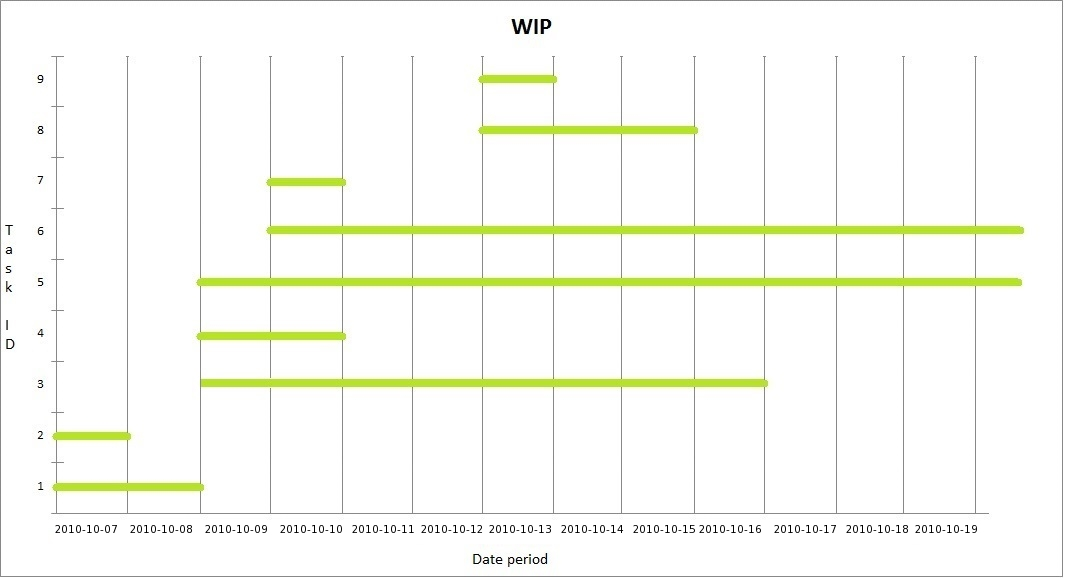
\includegraphics[width=21cm,trim=4 8 8 4,clip]{Picture/wip_example.jpg}
\caption{Illustrating the WIP timeline for example stated in section \ref{sec:Example}}
\label{wip_timeline}
\end{adjustwidth}
\end{figure}

\newpage
\begin{table}[!ht]
\begin{center}
    \begin{tabular}{| l | l | p{2cm} | l | l |}
    \hline
   Task ID &   Date From  & Date To & Team & Process Type\\ \hline
     1 & 2010-10-07 & 2010-10-08 & Team One & Kanban  \\ \hline
     2 & 2010-10-07 & 2010-10-07 & Team One & Kanban   \\ \hline
     3 & 2010-10-09 & 2010-10-16 & Team One & Kanban   \\ \hline
     4 & 2010-10-09 & 2010-10-10 & Team One & Kanban   \\ \hline
     5 & 2010-10-09 & 2010-11-04 & Team One & Kanban   \\ \hline
     6 & 2010-10-10 & 2010-11-05 & Team One & Kanban  \\ \hline
     7 & 2010-10-10 & 2010-10-10 & Team One & Kanban   \\ \hline
     8 & 2010-10-13 & 2010-10-15 & Team One & Kanban  \\ \hline
     9 & 2010-10-13 & 2010-10-13  & Team One  & Kanban   \\ \hline
    \end{tabular}
\caption{Showing Task ID, Date From and Date to}
\label{wt:2} %%  wip table 2\
\end{center}
\end{table}

\subsubsection{Step 1}
The program will first read in line 1 of table \ref{wt:2}.  Line 1 is labeled with task id one.  The program creates the WIP-object line 1 and it will look like the Listing \ref{lst:WIPOBJ}.  The program will follow the exact same procedure until all the dates are read. 

\begin{minipage}{\textwidth} 
\begin{lstlisting}[caption={Creating WIP-object},label={lst:WIPOBJ}]
WIP = new WIP()
WIP.start = 2010-10-07
WIP.end = 2010-10-08
WIP.team = "Team One"
WIP.processType = "Kanban"
WIP.WIP = 1
\end{lstlisting}
  \end{minipage}

 \subsubsection{Step 2}
\label{sub:sub:st}
Now that the whole set has been read and saved, the next thing to do is to create the remaining dates. The Arraylist contains all the dates from Table \ref{wt:2}.  The program will now extract the first and the last date from the Arraylist. Before this step, the objects in the Arraylist are sorted by date. The first date is 2010-10-07 and the last date is 2010-10-13.  The program will check if the date after 2010-10-07 contains in the set, which it does not. The program then generates a WIP object for the date 2010-10-08 and adds it to the Arraylist. % as shown in Listing \ref{lst:WIPCREATE}. 
After the date is created, the program will see if the date 2008-10-09 exits and will do so for the rest of the dates.

\iffalse
\begin{minipage}{\textwidth} 
\begin{lstlisting}[caption={Creating WIP-object},label={lst:WIPCREATE}]
void createNewWIP(Date d, String team) 
	WIP.start = d
	WIP.end = d
	WIP.team = team
	WIP.processType = "Unknown"
	WIP.WIP = 0
\end{lstlisting}
  \end{minipage}
\fi

\subsubsection{Step 3}
The Arraylist now contains the dates from 2010-10-08 to 2010-10-13. The next and last step is to measure WIP for each date.  The program will now loop through the Arraylists. The first date is 2010-10-07.  The get\_current\_wip method from line 9 in Listing \ref{lst:measure} will be called with the date 2010-10-07 as parameter.  The method will return two, because both tasks one and two were started at 2010-10-07 as shown by Figure \ref{wip_timeline}. The next thing to do is to find out how many tasks to decrement the current WIP with.  The method Nr\_of\_finished\_dates in line 17 is called with the date 2010-10-07. As shown by the Table \ref{wt:2} and Figure \ref{wip_timeline} there was no task finished at the date 2010-10-07, so the method returns 0. The program then updates the WIP objects' counter to be two and saves the WIP value in the lastWIP variable. The next date is 2010-10-08, which the program made in Subsection \ref{sub:sub:st}. There is no task started at 2010-10-08, but task one is finished at the date. So the Nr\_of\_finished\_dates returns one and flags the current date as shown in Listing \ref{lst:measure} by the line 23. The result of WIP\_measure in line 5 is 1 ($0-1+2=1$), therefore WIP at date 2010-10-08 is 1, as shown by Figure \ref{wip_timeline}. The program will continue this procedure until all the dates are measured.  The reason why the date is flagged is to be sure that each date is only evaluated ones.
\iffalse
\subsubsection{First step}
\label{subsubsec:ft}
The program will first do a look-up on the date 2008-10-07 referred with task ID one and two in table \ref{wt:2} and measure the current WIP counter, which is two, because its two tasks in progress on this date. After this the program will put the date and the current WIP into a Arraylist. 
Now the algorithm will see if any task was done in the last period, since task one and two is the two first tasks to be measured in this example, there's no task finished in the period and there's no current WIP from other tasks, so the current WIP at 2008-10-07 is two illustrated by Figure \ref{wip_timeline}. 
\subsubsection{Second step}
The program will do a look-up on the date 2008-10-09 referred with task ID three, four and five in table \ref{wt:2}  and measure the current WIP for this date, which is three. Then, the program will put the date and the current WIP into a Arraylist.
Next, the program will see that two tasks were done in the period of 2008-10-07 to 2008-10-09. So the program will measure that three new tasks were started at 2008-10-09, two where finished and the WIP from last date measure where two, so the calculation of WIP at 2008-10-09 is 3-2+2, which gives a WIP of three on 2008-10-09 illustrated by Figure \ref{wip_timeline}. 

\subsubsection{Third step}
The program will do a look-up on the date 2008-10-10 referred with task ID six and seven in table \ref{wt:2}  and measure the current WIP for this date, which is two. Next the program will put the date and the current WIP into a Arraylist.
Last the program will see that no task where done in the period 2008-10-09 to 2008-10-10 and the currently WIP is three, so this gives a new WIP of 5 illustrated by Figure \ref{wip_timeline}. 

\subsubsection{Fourth step}
The program will do a look-up on the date 2008-10-13 referred with task ID eight and nine in table \ref{wt:2}  and measure the current WIP for this date, which is two. Then the program will put the date and the current WIP into a Arraylist. 
Next the program will look at the period between 2008-10-10 and 2008-10-13, and see that task four and seven was done in this period. The WIP at 2008-10-13 will be $2-2+5 = 5$ as illustrated by Figure \ref{wip_timeline}. 
As illustrated by the example, WIPs are not decrement until the finished date is passed, even though the task is done on the date, it is also worked on the same date, therefore the WIP is decrement after each date is passed.
\fi

 \section{Rest of the variables}
 \label{sec:rotv}
To compute the remaining variables a new algorithm is required.  The first part of the algorithm for the remaining variables is identical. First the program reads in the data set from SI. For each of the lines in the data set, the program creates an object and saves the valuable information from the data set in the object. Then each object is saved in a data structure based on team association as showed in Listing \ref{addObj}.  After all the lines has been read and all objects has been put in the right data structure the algorithms differ. \begin{lstlisting}[caption=Pseudocode example of how throughput objects are added, label=addObj]
void addBug(Bug b)
	if b.team EQUALS "TeamOne"
		if dateExists(b.date, TeamOne) EQUALS false
			// if date does not exists, then add the bug
			TeamOne.add(b)
			
	if b.team EQUALS "TeamTwo"
		if dateExists(b.date, TeamTwo) EQUALS false
			// if date does not exists, then add the bug
			TeamTwo.add(b)
			
	if b.team EQUALS "TeamThree"
		if dateExists(b.date, TeamThree) EQUALS false 
			// if date does not exists, then add the bug
			TeamThree.add(b)
			
	if b.team EQUALS "TeamFour"
		if dateExists(b.date, TeamFour) EQUALS false
			// if date does not exists, then add the bug
			TeamFour.add(b)
			
			/* And so on for the rest of the teams */
		
	
 \end{lstlisting}
 
% void dateExists(Date d, Arraylist list)
%	for Bug b in list
%		if b.date EQUALS d
%			b.counter++
%	
%return false The method in line 24 assurance that only on object of each date is in the data structure
 
\subsection{Throughput}
 \label{sec:TP}
When the steps described in Section \ref{sec:rotv} are finished, the program takes the teams data structures and compute throughput. To compute throughput, a counter representing the throughput for each date is created. The method dateExists in Listing \ref{throughputCode} does the actual computation. The method starts of with a test. If the date of the throughput object is in the data structure, the corresponding counter is incremented.  If the date is not in the data structure, the new throughput object is added to the data structure.
 
\begin{minipage}{\textwidth}
\begin{lstlisting}[caption=Pseudocode example of how throughput is measured, label=throughputCode]
void dateExists(Throughput tp, Arraylist list)
	for Throughput t in list
		if t.date EQUALS tp.date
			t.counter++
			return
			
	structure.add(tp);
\end{lstlisting}
 \end{minipage}


\subsection{Churn}
\label{sec:churn}
As stated in Section \ref{sec:Churn} in order to take churn into account one has to know its good surrogates. SI has gathered churn with help of Microsoft's Team Foundation Server (TFS) \parencite{Dag}. The TFS system automatically records data such as churn and lead time. Based on TFS one can know that churn for SI is a good surrogate.

To measure churn the data set from SI contains three columns ("Lines added, "Lines modified" and "Lines deleted") shown in Table \ref{table:churn}. These three variables are summed together and saved in a  variable called "churn".  For example; for task id 1 the churn is 2028 ($352+307+1369 = 2028$). Some tasks has zero churn, for example task with id 6, these tasks do not need code in order to be finished such tasks need technical support to be finished. The churn algorithm is shown in Listing \ref{churnCode}

\begin{table}[!ht]
\begin{center}
    \begin{tabular}{| l | l | l | l |}
    \hline
\bf{Task id} & \bf{Lines added} & \bf{Lines modified}  & \bf{Lines deleted} \\ \hline
1&352&307&1369\\ \hline
2&314 & 31 & 15 \\ \hline
3&314&31 & 15\\ \hline
4&62&327&153 \\ \hline
5&21&3&0 \\ \hline
6&0&0&0 \\ \hline
\end{tabular}
\caption{How churn is presented in the excel document}
\label{table:churn} %%  bugs table
\end{center}
\end{table}

\begin{minipage}{\textwidth}
\begin{lstlisting}[caption=Pseudocode example of how throughput is measured, label=churnCode]
void updateChurn(Churn c, Arraylist list)
	for Churn ch in list
		if ch.date EQUALS c.date
			ch.churn += c.churn
			return
	structure.add(c);
\end{lstlisting}
 \end{minipage}
 


\subsection{Lead time}
\label{sec:LT}
The program does not need to analyze  the lead time for each task. The lead time for each task is recorded by TFS. The lead time is represented in the data set by a column as shown in Table \ref{table:LT}. The program will gather all the tasks that are started on the same date and belong to the same team and add up their lead time together as showed in code Listing \ref{LTcode}.   
\begin{table}[!ht]
\begin{center}
\begin{tabular}{ | l | l | l | }
\hline
	\bf{ID} & \bf{Type} & \bf{Lead time} \\ \hline
	84096 &  Feature  & 1 \\ \hline
	84118 &  Bug  & 25 \\ \hline
	84096 &  Feature  & 7 \\ \hline
	84118 &  Bug  & 13 \\ \hline
\end{tabular}
\caption{How lead time is recorded in the excel document}
\label{table:LT} %%  bugs table
\end{center}
\end{table}

\begin{minipage}{\textwidth}
\begin{lstlisting}[caption=Pseudocode example of lead time is measured, label=LTcode]

addLeadTime(Leadtime t, Arraylist list)
	for lead_time in list
		if lead_time.date EQUALS t.date
			lead_time.lead time+= t.lead time
			return
			
	structure.add(t)
\end{lstlisting}
\end{minipage}
\subsection{Lead time and churn}
As stated in the paper "Quantifying the Effect of Using Kanban versus Scrum" \parencite{Dag} to prevent outliers from having a large effect on the results, the top and lowest ten percent of lead time and churn are removed from the data set.
Churn is removed because a module or a feature, which consists of hundreds or thousands of lines of code could be removed without much work. Lead time is removed because some tasks could be given low priority due to lack of manpower in a given period. Or, tasks could be labeled as not critical and the lead time of these tasks will effect the result.

\subsection {Sub variables}
\label{sec:bug}
To measure sub variables, the software program and SPSS was used. The program will generate throughput and churn as described in Sections \ref{sec:TP} and \ref{sec:churn}, the output from the software program will look like Table \ref{tab:ftb}. The output from the program will be used by SPSS. SPSS will use a function called case summaries, the case summaries function groups variables based on a common value.  With the case summaries function the variable "Team name", "Quarter" and "Type" will be grouped by churn and throughput. The result from case summaries provides the sub variables for each quarter.
\begin{table}[!ht]
\center
\begin{tabular}{ | l | l | l | l | l |l | }
\hline
	\bf{Team name} & \bf{Churn} &\bf{Throughput} & \bf{Date} & \bf{Quarte}r & \bf{Type} \\ \hline
	Team one & 25 &10&2011-12-20& 2011-4 & Feature \\ \hline
	Team two & 3 &5&2012-04-19 & 2012-2 & bug \\ \hline
	Team one & 7 &2& 2010-08-06 & 2010-3 & Feature \\ \hline
\end{tabular}
\caption{A excerpt from the result data produced by the program }
\label{tab:ftb} 
\end{table}

\subsection{Bugs finished, quarter}
\label{sub:sec:bfq} 
To get the statistics on number of bugs finished the same quarter as it was recorded, the software program and SPSS was used. The program extracted the "created date" and the "date to" values from each task and checks if their quarters match. If they do, a boolean value is set to true, otherwise it is set to false. The output is used in SPSS, where the boolean value is grouped together with "Team name" and "Quarter". After the SPSS has measured, the number of finished bugs is divided by the total in order to find the percentages of bugs finished within a quarter. 
\subsection{Average days backlog, bug}
\label{sub:sec:adbb}
To get the statistics on the average number of days bugs are in backlog per quarter, the program measures the number of days between the created date and the date from value. The number of days is saved together with the task. SPSS is used on the output of the program to measure the average days backlog for bugs variable.

The sub variables, bugs finished, quarter and average days backlog, bug is used as help variables. These variables will not have their own correlation table. 
% If bugs are longer in backlog or the average days of bugs in backlog is decreasing, depends on the bugs, throughput or the lead time variable. 

\section{Summary}
This chapter presented the algorithm and an example of how WIP is computed in this work as well as how the other variables are computed.


\chapter{Results}                     
\label{ch:res}
The first correlation result showed an average correlation value  of 0.6 between \textit{team size} and \textit{WIP} and 0.5 between \textit{team size} and \textit{throughput}. Five of the ten teams also had a significant positive correlation between these variables. Based on the correlation values, it was hard to find any evidence if WIP-limit matters in software development. This resulted in a new analyze where each variable for each quarter was divided by the corresponding team size. 

Each section except Section \ref{sec:corr:tz} "Team size"  and Section \ref{sec:corr:alc} "All teams combined" is presented with two correlation tables and two corresponding descriptive statistics tables, one correlation table and descriptive statistic table for the first analysis and the same two tables for the second analyze. {Team size} is presented with one correlation table and one descriptive statistic table, while all teams combined is presented  with one correlation table for the two analyzes. The content of the sections will consist of highlighting the variables with a significant correlation and describe the descriptive statistic tables.
\section{Correlation - WIP}
\label{sec:corr:WIP}
Table \ref{corr:WIP} displays the first correlation tables for \textit{WIP}. The variables are listed vertically in the correlation table. Horizontally are the corresponding teams. The team names are shortened, team one is shortened to T1, team two is shortened to T2 and so on.
The correlation Table \ref{corr:WIP} shows \textbf{team one} has a positive correlation to \textit{throughput}, \textit{throughput feature}, \textit{bugs}, \textit{lead time}, \textit{churn feature} and \textit{team size}. \textbf{Team two} has a significant negative correlation value to \textit{churn} and \textit{churn bug}. \textbf{Team three} has a positive correlation value to all \textit{throughput} variables, \textit{bugs} and \textit{team size}. \textbf{Team four} has significant positive correlation to all variables except \textit{team size}. \textbf{Team five} has a positive correlation to \textit{throughput bug}, \textit{lead time} and \textit{team size}.


\begin{table}[H]
 \begin{adjustwidth}{-3cm}{}
 \centering
 \begin{tabular}{|l|r|r|r|r|r|r|r|r|r|r|}
\hline
 & \bf{T1} & \bf{T2} & \bf{T3} & \bf{T4} & \bf{T5} & \bf{T6} & \bf{T7} & \bf{T8} & \bf{T9} & \bf{T10}\\ \hline
 Throughput  & 0.74** & 0.21 & 0.76** & 0.83** & 0.52 & 0.64* & 0.67* & 0.47 & 0.89** & 0.61* \\ \hline
 Throughput Feature  & 0.73** & -0.14 & 0.83** & 0.82** & 0.25 & 0.68** & 0.63* & 0.56* & 0.82** & 0.20 \\ \hline
 Throughput bug  & 0.02 & 0.25 & 0.73** & 0.56* & 0.54* & 0.07 & 0.55 & 0.15 & 0.88** & 0.63* \\ \hline
 Bugs  & 0.72** & 0.20 & 0.60* & 0.74** & 0.50 & 0.46 & 0.62 & 0.04 & 0.58* & 0.18 \\ \hline
 Bugs finished, quarter  & 0.35 & 0.10 & -0.07 & 0.56* & 0.19 & 0.19 & 0.85** & 0.23 & 0.52 & 0.35 \\ \hline
 Avg days in backlog, bugs  & -0.03 & 0.44 & 0.42 & 0.54* & -0.18 & 0.02 & 0.10 & 0.14 & -0.20 & -0.18 \\ \hline
 Lead time  & 0.75** & 0.46 & 0.49 & 0.70** & 0.57* & 0.29 & 0.68* & 0.16 & 0.23 & 0.72** \\ \hline
 Churn  & 0.47 & -0.71** & -0.32 & 0.66* & 0.03 & -0.30 & 0.15 & 0.16 & -0.09 & 0.16 \\ \hline
 Churn feature  & 0.72** & -0.25 & -0.34 & 0.72** & 0.06 & -0.36 & 0.10 & 0.20 & -0.12 & 0.32 \\ \hline
 Churn bug  & 0.15 & -0.60* & -0.52 & 0.62* & 0.11 & 0.77** & -0.05 & -0.22 & -0.30 & -0.10 \\ \hline
 Team size  & 0.68** & 0.35 & 0.78** & 0.06 & 0.57* & 0.77** & 0.62 & 0.65* & 0.54 & 0.76**\\ \hline
\end{tabular}
 \caption{Correlation - WIP - When team size is \textbf{not} taken into account}
\label{corr:WIP}
 \centerline {* Correlation is significant at the 0.05 level (2-tailed).}
\centerline{** Correlation is significant at the 0.01 level (2-tailed).}
\end{adjustwidth}
\end{table}

\textbf{Team six} has a positive correlation to \textit{throughput, throughput feature, churn bug} and \textit{team size}. \textbf{Team seven} has a positive correlation to \textit{throughput, throughput feature}, \textit{bugs finished, quarter} and \textit{lead time}. \textbf{Team eight} has a positive correlation value to \textit{throughput feature} and \textit{team size}. \textbf{Team nine} has positive correlation value to the three \textit{throughput} variables and \textit{bugs}. \textbf{Team ten} has a positive correlation to \textit{throughput, throughput bug, lead time} and \textit{team size}. 

\textit{Throughput feature}, \textit{throughput bug}, \textit{churn feature} and \textit{churn bug} is subset of 
respectively \textit{throughput} and \textit{churn}. It is natural that these sub variables have a significant positive correlation to \textit{WIP}, when either \textit{throughput}  or  \textit{churn} has. That's not the case for all teams. 
There is a gap in the relationship between the \textit{churn} variables and \textit{throughput} variables for both team \textbf{one} and \textbf{six}. The \textit{throughput} variables for teams \textbf{five, seven, eight} and \textbf{ten} also have a gap, the same goes for the \textit{churn} variables for \textbf{team two},  showed by Table \ref{corr:WIP}.  The relationship between these variables is explained in Section \ref{sec:diss:sv}.


The descriptive statistics tables in each section are based on summary of the correlation values. The tables show number of values measured (N), mean, median, standard deviation (Std.dev), maximum (Max)  and minimum (Min) values from the correlation tables.
In Table \ref{DS:corr:WIP}, the mean correlation value for \textit{throughput} and \textit{team size} is 0.6. The mean correlation value for \textit{lead time, throughput feature, throughput bug and bugs} is 0.5 and \textit{bugs finished, quarter} has an value of 0.3. Rest of the values has a mean value of $\pm$ 0.2 or less.
\begin{minipage}[t]{\linewidth}
\begin{table}[H]
 \centering
 \begin{tabular}{ | l | r | r | r | r | r | r | }
 \hline
& \bf{N} & \bf{Mean} & \bf{Median} & \bf{Std.Dev} & \bf{Max} & \bf{Min} \\ \hline
Throughput  & 10 & 0.6 & 0.7 & 0.2 & 0.9 & 0.2\\ \hline
Throughput ft  & 10 & 0.5 & 0.7 & 0.3 & 0.8 & -0.1\\ \hline
Throughput bug  & 10 & 0.5 & 0.5 & 0.3 & 0.9 & 0\\ \hline
Bugs  & 10 & 0.5 & 0.5 & 0.2 & 0.7 & 0\\ \hline
Bugs finished, quarter  & 10 & 0.3 & 0.3 & 0.3 & 0.9 & -0.1\\ \hline
Avg days backlog, bugs  & 10 & 0.1 & 0.1 & 0.3 & 0.5 & -0.2\\ \hline
Lead time & 10 & 0.5 & 0.5 & 0.2 & 0.7 & 0.2\\ \hline
Churn  & 10 & 0 & 0.1 & 0.4 & 0.7 & -0.7\\ \hline
Churn ft  & 10 & 0.1 & 0.1 & 0.4 & 0.7 & -0.4\\ \hline
Churn bug  & 10 & -0 & -0 & 0.4 & 0.8 & -0.6\\ \hline
Team size  & 10 & 0.6 & 0.6 & 0.2 & 0.8 & 0.1\\ \hline
\end{tabular}
 \caption{Descriptive Statistic - Correlation - WIP - When team size is \textbf{not} taken into account}
 \label{DS:corr:WIP}
 \end{table}
\end{minipage} 

In Table \ref{corr:WIP:V2}, \textbf{team two} has a significant positive correlation between \textit{WIP} and \textit{throughput}, \textit{throughput bug},  \textit{bugs finished, quarter} and \textit{lead time}. \textbf{Team three} has a significant positive correlation value between \textit{WIP} and \textit{throughput, throughput feature} and a significant negative correlation for \textit{bugs finished, quarter}. \textbf{Team four} has a positive correlation between all variables except \textit{throughput bug, bugs}, \textit{avg days in backlog, bugs} and \textit{churn bug}. 



\begin{table}[H]
  \begin{adjustwidth}{-1.5cm}{}
 \center
  \captionsetup{justification=centering}
 \begin{tabular}{|l|r|r|r|r|r|r|r|r|r|r|}
\hline
 &  \bf{T1} & \bf{T2} & \bf{T3} & \bf{T4} & \bf{T5} & \bf{T6} & \bf{T7} & \bf{T8} & \bf{T9} & \bf{T10}\\ \hline
 Throughput  & 0.37 & 0.59* & 0.57* & 0.86** & 0.11 & 0.08 & 0.49 & 0.28 & 0.66* & -0.21 \\ \hline
 Throughput Feature  & 0.31 & 0.47 & 0.71** & 0.85** & 0 &0.14 & 0.46 & -0.26 & 0.60* & -0.16 \\ \hline
 Throughput bug  & 0.09 & 0.65* & 0.52 & 0.27 & 0.11 & 0.07 & 0.57 & 0.37 & 0.58* & -0.22 \\ \hline
 Bugs  & 0.10 & 0.49 & 0.25 & 0.25 & 0.11 & 0.25 & 0.75* & 0.32 & -0.05 & -0.28 \\ \hline
 Bugs finished, quarter  & -0.28 & 0.71** & -0.62* & 0.74** & -0.24 & -0.04 & 0.85** & 0.82** & 0.32 & -0.28 \\ \hline
 Avg days in backlog, bugs  & 0.03 & -0.31 & 0.51 & 0.10 & -0.14 & 0 &0.16 & -0.17 & -0.40 & -0.61* \\ \hline
 Lead time  & -0.09 & 0.67** & -0.03 & 0.87** & 0.03 & 0.32 & 0.77* & -0.09 & -0.18 & -0.05 \\ \hline
 Churn  & -0.27 & 0.16 & -0.29 & 0.77** & -0.09 & -0.35 & -0.17 & 0.39 & -0.34 & -0.37 \\ \hline
 Churn feature  & 0.37 & 0.03 & -0.38 & 0.78** & -0.15 & -0.39 & -0.17 & -0.04 & -0.17 & 0.08 \\ \hline
 Churn bug  & -0.29 & 0.21 & -0.39 & 0.26 & -0.07 & 0.12 & -0.17 & 0.66* & -0.49 & -0.43 \\ \hline
\end{tabular}
 \caption{Correlation - WIP - When team size is taken into account}
 \label{corr:WIP:V2}
 \centerline {* Correlation is significant at the 0.05 level (2-tailed).}
\centerline{** Correlation is significant at the 0.01 level (2-tailed).}
\end{adjustwidth}
\end{table}

\textbf{Team seven} has a significant positive correlation for \textit{bugs}, \textit{bugs, finished quarter} and \textit{lead time}. \textbf{Team eight} has a significant correlation for \textit{bugs finished, quarter} and \textit{churn bug}. \textbf{Team nine} has a significant positive correlation to all \textit{throughput} variables. \textbf{Team ten} has a significant negative correlation for \textit{avg days in backlog, bugs}.

In Table \ref{corr:WIP:V2}, teams \textbf{two} and \textbf{three} have a significant correlation value for two of the three \textit{throughput} variables. \textbf{Team four} has a positive correlation for two of the three \textit{churn} and \textit{throughput} variables and \textbf{team eight} has significant correlation to one \textit{churn} of the three \textit{churn} variables. The relationship between these sub variables is explained in Section \ref{sec:diss:sv}. The descriptive statistic Table \ref{DS:corr:WIP:v2} shows \textit{throughput} has an average correlation value of 0.4. The rest of the variables except \textit{throughputs} sub variables have an average correlation values $\pm$ 0.2 or less. 


\begin{minipage}[t]{\linewidth}
\begin{table}[H]
 \centering
 \begin{tabular}{ | l | r | r | r | r | r | r | }
 \hline
& \bf{N} & \bf{Mean} & \bf{Median} & \bf{Std.Dev} & \bf{Max} & \bf{Min} \\ \hline
Throughput  & 10 & 0.4 & 0.4 & 0.3 & 0.9 & -0.2\\ \hline
Throughput ft  & 10 & 0.3 & 0.4 & 0.4 & 0.9 & -0.3\\ \hline
Throughput bug  & 10 & 0.3 & 0.4 & 0.3 & 0.7 & -0.2\\ \hline
Bugs  & 10 & 0.2 & 0.2 & 0.3 & 0.8 & -0.3\\ \hline
Bugs finished, quarter  & 10 & 0.2 & 0.1 & 0.6 & 0.8 & -0.6\\ \hline
Avg days backlog, bugs  & 10 & -0.1 & -0.1 & 0.3 & 0.5 & -0.6\\ \hline
Lead time & 10 & 0.2 & 0 & 0.4 & 0.9 & -0.2\\ \hline
Churn  & 10 & -0.1 & -0.2 & 0.4 & 0.8 & -0.4\\ \hline
Churn ft  & 10 & 0 & -0.1 & 0.4 & 0.8 & -0.4\\ \hline
Churn bug  & 10 & -0.1 & -0.1 & 0.4 & 0.7 & -0.5\\ \hline
\end{tabular}
 \caption{Descriptive Statistic - Correlation - WIP - When team size is taken into account}
 \label{DS:corr:WIP:v2}
 \end{table}
\end{minipage}

\section{Correlation - Lead time}
\label{sec:corr:lt}
Table \ref{corr:lt} displays the first correlation table for \textit{lead time}. \textbf{Team one} has a positive correlation for all variables except \textit{throughput bug}, \textit{avg days in backlog, bugs} and \textit{churn bug}. \textbf{Team two} has a positive correlation value to \textit{throughput} and \textit{throughput bug}. \textbf{Team three} has a positive correlation value to \textit{bugs} and a negative correlation value to \textit{churn bug}. \textbf{Team four} has a significant positive correlation value to \textit{WIP}, \textit{throughput, throughput feature}  \textit{churn} and \textit{churn feature}. \textbf{Team five} has a significant correlation value to \textit{WIP}.

\begin{minipage}[t]{\linewidth}
\begin{table}[H]
 \begin{adjustwidth}{-1.5cm}{}
 \centering
 \begin{tabular}{|l|r|r|r|r|r|r|r|r|r|r|}
\hline
 & \bf{T1} & \bf{T2} & \bf{T3} & \bf{T4} & \bf{T5} & \bf{T6} & \bf{T7} & \bf{T8} & \bf{T9} & \bf{T10}\\ \hline
 WIP  & 0.75** & 0.46 & 0.49 & 0.70** & 0.57* & 0.29 & 0.68* & 0.16 & 0.23 & 0.72** \\ \hline
 Throughput  & 0.70** & 0.67** & 0.49 & 0.68** & 0.36 & 0.13 & 0.47 & 0.54 & 0.42 & 0.32 \\ \hline
 Throughput Feature  & 0.73** & 0.09 & 0.44 & 0.64* & 0.14 & 0.10 & 0.41 & 0.62* & 0.41 & -0.05 \\ \hline
 Throughput bug  & -0.30 & 0.60* & 0.52 & 0.31 & 0.42 & -0.01 & 0.61 & -0.17 & 0.28 & 0.37 \\ \hline
 Bugs  & 0.77** & 0.50 & 0.54* & 0.22 & 0.32 & -0.23 & 0.69* & -0.13 & 0.44 & 0.04 \\ \hline
 Bugs finished, quarter  & 0.70** & -0.14 & 0.20 & 0.23 & -0.09 & -0.27 & 0.73* & 0.37 & 0.53 & 0.19 \\ \hline
 Avg days in backlog, bugs  & 0.06 & 0.40 & 0.07 & 0.07 & -0.08 & -0.03 & 0.57 & -0.12 & -0.48 & -0.52 \\ \hline
 Churn  & 0.70** & -0.42 & -0.45 & 0.97** & 0.18 & -0.34 & 0.37 & 0.91** & -0.37 & -0.04 \\ \hline
 Churn feature  & 0.86** & 0.20 & -0.27 & 0.96** & 0.11 & -0.31 & 0.39 & 0.79** & -0.46 & 0.32 \\ \hline
 Churn bug  & 0.26 & -0.39 & -0.64* & 0.20 & 0.24 & 0.28 & 0.16 & -0.12 & -0.08 & -0.27 \\ \hline
 Team size  & 0.61* & 0.38 & 0.44 & -0.30 & 0.36 & -0.11 & 0.59 & 0.22 & 0.38 & 0.53 \\ \hline
\end{tabular}
 \caption{Correlation - Lead time - Without taken time size into account}
 \label{corr:lt}
 \centerline {* Correlation is significant at the 0.05 level (2-tailed).}
\centerline{** Correlation is significant at the 0.01 level (2-tailed).}
\end{adjustwidth}
\end{table}
\end{minipage}

\textbf{Team seven} has a significant positive correlation value to \textit{WIP}, \textit{bugs} and \textit{bugs finished, quarter}. \textbf{Team eight} has a significant correlation value to \textit{throughput feature}, \textit{churn} and \textit{churn feature}. \textbf{Team ten} has a significant correlation value with \textit{WIP}.

Table \ref{corr:lt} displays the variances between the \textit{throughput} variables for team \textbf{one, two, four} and \textbf{eight}. There is also variance for the \textit{churn} variables for team \textbf{one, three, four} and \textbf{eight}. The relationship between these variables is explained in Section \ref{sec:diss:sv}. Table \ref{DS:corr:LT} shows the average correlation value of 0.5 for \textit{WIP} and \textit{throughput}. \textit{Throughput feature} has the average correlation value of 0.4 and \textit{throughput bug, bugs, churn feature} and \textit{team size} has the average value of 0.3 and rest of the values has a value of $\pm$ 0.2 or less.



\begin{table}[H]
 \centering
 \begin{tabular}{ | l | r | r | r | r | r | r | }
 \hline
 & \bf{N} & \bf{Mean} & \bf{Median} & \bf{Std.Dev} & \bf{Max} & \bf{Min} \\ \hline
WIP  & 10 & 0.5 & 0.5 & 0.2 & 0.7 & 0.2\\ \hline
Throughput  & 10 & 0.5 & 0.5 & 0.2 & 0.7 & 0.1\\ \hline
Throughput ft  & 10 & 0.4 & 0.4 & 0.3 & 0.7 & -0.1\\ \hline
Throughput bug  & 10 & 0.3 & 0.4 & 0.3 & 0.6 & -0.3\\ \hline
Bugs  & 10 & 0.3 & 0.4 & 0.3 & 0.8 & -0.2\\ \hline
Bugs finished, quarter  & 10 & 0.2 & 0.2 & 0.3 & 0.7 & -0.3\\ \hline
Avg days backlog, bugs  & 10 & 0 & 0 & 0.3 & 0.6 & -0.5\\ \hline
Churn  & 10 & 0.2 & 0.1 & 0.6 & 1 & -0.5\\ \hline
Churn ft  & 10 & 0.3 & 0.3 & 0.5 & 1 & -0.5\\ \hline
Churn bug  & 10 & -0.1 & -0.1 & 0.3 & 0.3 & -0.6\\ \hline
Team size  & 10 & 0.3 & 0.4 & 0.3 & 0.6 & -0.3\\ \hline
\end{tabular}
 \caption{Descriptive Statistic - Correlation - Lead time - Without taken time size into account}
 \label{DS:corr:LT}
 \end{table}

Table \ref{corr:LT:V2} displays the second correlation table. \textbf{Team one} has significant positive correlation for \textit{bugs}, \textit{bugs finished, quarter}, \textit{churn} and \textit{churn bug}. \textbf{Team two} has a significant positive correlation for  \textit{WIP}, \textit{throughput} variables, \textit{bugs}, \textit{bugs finished, quarter} and \textit{churn bug}.  \textbf{Team four} has a significant positive correlation for \textit{WIP}, \textit{throughput, throughput feature}, \textit{churn} and \textit{churn feature}. \textbf{Team five} has significant correlation value to \textit{throughput}, \textit{throughput bug}, \textit{bugs}, \textit{bugs, finished, quarter}, \textit{avg days in backlog, bugs}, \textit{churn} and \textit{churn bug}.


\begin{table}[H]
  \begin{adjustwidth}{-2.5cm}{}
 \centering
 \begin{tabular}{|l|r|r|r|r|r|r|r|r|r|r|}
\hline
 &  \bf{T1} & \bf{T2} & \bf{T3} & \bf{T4} & \bf{T5} & \bf{T6} & \bf{T7} & \bf{T8} & \bf{T9} & \bf{T10}\\ \hline
 WIP  & -0.09 & 0.67** & -0.03 & 0.87** & 0.03 & 0.32 & 0.77* & -0.09 & -0.18 & -0.05 \\ \hline
 Throughput  & 0.06 & 0.88** & 0.26 & 0.90** & 0.80** & 0.69** & 0.33 & 0.24 & 0.32 & 0.90** \\ \hline
 Throughput Feature  & 0.01 & 0.75** & 0.16 & 0.89** & -0.05 & 0.61* & 0.34 & 0.87** & 0.20 & -0.26 \\ \hline
 Throughput bug  & 0.51 & 0.84** & 0.29 & 0.22 & 0.84** & 0.41 & 0.56 & -0.27 & 0.25 & 0.91** \\ \hline
 Bugs  & 0.83** & 0.72** & 0.48 & 0.44 & 0.72** & 0.18 & 0.85** & -0.23 & 0.54 & 0.88** \\ \hline
 Bugs finished, quarter  & 0.88** & 0.79** & 0.32 & 0.52 & 0.80** & 0.36 & 0.77** & -0.04 & 0.45 & 0.57* \\ \hline
 Avg days in backlog, bugs  & 0.41 & -0.52 & -0.04 & -0.07 & 0.85** & -0.09 & 0.51 & -0.20 & -0.17 & 0.10 \\ \hline
 Churn  & 0.72** & 0.49 & 0.16 & 0.96** & 0.94** & 0.04 & 0.08 & 0.71** & -0.18 & 0.01 \\ \hline
 Churn feature  & -0.52 & 0.38 & 0.22 & 0.96** & -0.21 & 0.11 & 0.05 & 0.86** & -0.28 & -0.24 \\ \hline
 Churn bug  & 0.73** & 0.55* & 0.07 & 0.13 & 0.95** & -0.17 & -0.06 & -0.12 & 0.24 & 0.03 \\ \hline
\end{tabular}
 \caption{Correlation - Lead time - With team size taken into account}
 \label{corr:LT:V2}
 \centerline {* Correlation is significant at the 0.05 level (2-tailed).}
\centerline{** Correlation is significant at the 0.01 level (2-tailed).}
\end{adjustwidth}
\end{table}

\textbf{Team six} has a significant correlation for \textit{throughput} and \textit{throughput feature}. \textbf{Team seven} has a significant correlation for \textit{WIP}, \textit{bugs} and \textit{bugs, finished, quarter}. \textbf{Team eight} has a significant correlation for \textit{throughput feature}, \textit{churn} and \textit{churn feature}. \textbf{Team ten} has a significant positive correlation for \textit{throughput}, \textit{throughput bug} and \textit{bugs}.  

The \textit{throughput} relationship for team \textbf{four, five, six, eight} and \textbf{ten} show variances according to Table \ref{corr:LT:V2}. \textit{Churn} variables also show variances for team \textbf{one, two, four, five} and \textbf{eight}. The relationship between the variables is  explained in Section \ref{sec:diss:sv}.
The Table \ref{DS:corr:LT:v2} displays an average correlation value of 0.5 for  \textit{throughput}, \textit{throughput bug}, \textit{bugs} and \textit{bugs finished, quarter}. \textit{Churn} and \textit{throughput feature} has the average value of 0.4. The rest of the values have an average correlation value of $\pm$ 0.2 or less.



\begin{table}[H]
 \centering
 \begin{tabular}{ | l | r | r | r | r | r | r | }
 \hline
& \bf{N} & \bf{Mean} & \bf{Median} & \bf{Std.Dev} & \bf{Max} & \bf{Min} \\ \hline
WIP  & 10 & 0.2 & 0 & 0.4 & 0.9 & -0.2\\ \hline
Throughput  & 10 & 0.5 & 0.5 & 0.3 & 0.9 & 0.1\\ \hline
Throughput ft  & 10 & 0.4 & 0.3 & 0.4 & 0.9 & -0.3\\ \hline
Throughput bug  & 10 & 0.5 & 0.5 & 0.4 & 0.9 & -0.3\\ \hline
Bugs  & 10 & 0.5 & 0.6 & 0.4 & 0.9 & -0.2\\ \hline
Bugs finished, quarter  & 10 & 0.5 & 0.5 & 0.3 & 0.9 & -0\\ \hline
Avg days backlog, bugs  & 10 & 0.1 & -0.1 & 0.4 & 0.8 & -0.5\\ \hline
Churn  & 10 & 0.4 & 0.3 & 0.4 & 1 & -0.2\\ \hline
Churn ft  & 10 & 0.1 & 0.1 & 0.5 & 1 & -0.5\\ \hline
Churn bug  & 10 & 0.2 & 0.1 & 0.4 & 1 & -0.2 \\ \hline
\end{tabular}
 \caption{Descriptive Statistic - Correlation - Lead time - With team size taken into account}
 \label{DS:corr:LT:v2}
 \end{table}


\section{Correlation - Bugs}
\label{sec:corr:bug}
This section contains information about the correlation tables between the variables and \textit{bugs}. In the first correlation 
Table \ref{corr:bug}, one can see \textbf{team one} has a significant correlation value with all the variables except \textit{throughput bug}, \textit{bugs finished, quarter}, \textit{avg days in backlog, bugs}, and \textit{churn bug}. \textbf{Team two} has a significant correlation with \textit{throughput} and \textit{throughput bug}. \textbf{Team three} has a significant correlation with \textit{WIP}, the \textit{throughput} variables and \textit{lead time}. \textbf{Team four} has a significant correlation value with \textit{WIP}, \textit{throughput bug}, \textit{bugs finished, quarter}, \textit{avg days in backlog, bugs} and \textit{churn bug}. \textbf{Team five} has a significant correlation value with the \textit{throughput} variables and \textit{team size}. 

\begin{table}[h]
 \begin{adjustwidth}{-2.5cm}{}
 \centering
 \begin{tabular}{|l|r|r|r|r|r|r|r|r|r|r|}
\hline
 &  \bf{T1} & \bf{T2} & \bf{T3} & \bf{T4} & \bf{T5} & \bf{T6} & \bf{T7} & \bf{T8} & \bf{T9} & \bf{T10}\\ \hline
 WIP  & 0.72** & 0.20 & 0.60* & 0.74* & 0.50 & 0.46 & 0.62 & 0.04 & 0.58* & 0.18 \\ \hline
 Throughput  & 0.69** & 0.81** & 0.88** & 0.51 & 0.97** & 0.27 & 0.53 & 0.41 & 0.70** & 0.56* \\ \hline
 Throughput Feature  & 0.74** & 0.01 & 0.82** & 0.53 & 0.88** & 0.30 & 0.56 & 0.22 & 0.60* & -0.14 \\ \hline
 Throughput bug  & -0.17 & 0.83** & 0.87** & 0.54* & 0.96** & 0.69** & 0.50 & 0.92** & 0.65* & 0.59* \\ \hline
 Bugs finished, quarter  & 0.50 & -0.18 & 0.12 & 0.87** & 0.17 & 0.76** & 0.79** & 0.18 & 0.70** & 0.05 \\ \hline
 Avg days in backlog, bugs  & 0.52 & 0.38 & 0.43 & 0.53* & 0.18 & 0.24 & 0.23 & 0.28 & 0.21 & 0.13 \\ \hline
 Lead time  & 0.77** & 0.50 & 0.54* & 0.22 & 0.32 & -0.23 & 0.69* & -0.13 & 0.44 & 0.04 \\ \hline
 Churn  & 0.62* & -0.27 & 0.10 & 0.12 & -0.06 & -0.12 & 0.11 & -0.16 & -0.48 & 0.04 \\ \hline
 Churn feature  & 0.77** & 0.01 & 0.09 & 0.22 & 0.43 & -0.10 & 0.11 & -0.25 & -0.62* & 0.07 \\ \hline
 Churn bug  & 0.42 & -0.19 & -0.19 & 0.71* & -0.11 & 0.42 & 0.12 & 0.65* & -0.04 & 0\\ \hline
 Team size  & 0.80** & 0.26 & 0.27 & 0.06 & 0.71** & 0.41 & 0.41 & 0.42 & 0.41 & 0.16 \\ \hline
\end{tabular}
 \caption{Correlation - Bugs - Without team size is taken into account}
 \label{corr:bug}
 \centerline {* Correlation is significant at the 0.05 level (2-tailed).}
\centerline{** Correlation is significant at the 0.01 level (2-tailed).}
\end{adjustwidth}
\end{table}
\newpage
\textbf{Team six} has a significant correlation value with \textit{throughput bug} and \textit{bugs finished, quarter}. \textbf{Team seven} has a significant value with \textit{bugs finished, quarter} and \textit{lead time}. \textbf{Team eight} has a significant correlation relationship with \textit{throughput bug} and \textit{churn bug}. \textbf{Team nine} has a significant correlation relationship to \textit{WIP}, the \textit{throughput} variables, \textit{bugs finished, quarter} and \textit{churn feature}. \textbf{Team ten} has significant correlation with \textit{throughput} and \textit{throughput bug}.

Teams \textbf{one, four} and \textbf{eight} have variances in both the \textit{throughput} and \textit{churn} variables according to Table \ref{corr:bug}. Teams \textbf{two} and \textbf{ten} also have variances for the \textit{throughput} variables, while \textbf{team nine} has a variances between the \textit{churn} variables. The relationship between these variables is explained in  Section \ref{sec:diss:sv}.
In Table \ref{DS:corr:Bugs}, one can see that \textit{throughput} and \textit{throughput bug} has the average correlation value of 0.6, \textit{throughput feature} has the value 0.5, \textit{WIP} has an average correlation value of 0.4,  \textit{Bugs finished, quarter}, \textit{avg days backlog, bugs}, \textit{lead time} and \textit{team size} has the average correlation value of 0.3 and the \textit{churn} variables have the average  mean values of $\pm$ 0.2 or less.

\begin{table} [h]
 \centering
 \begin{tabular}{ | l | r | r | r | r | r | r | }
 \hline
& \bf{N} & \bf{Mean} & \bf{Median} & \bf{Std.Dev} & \bf{Max} & \bf{Min} \\ \hline
WIP  & 10 & 0.4 & 0.5 & 0.2 & 0.7 & 0\\ \hline
Throughput  & 10 & 0.6 & 0.6 & 0.2 & 1 & 0.3\\ \hline
Throughput ft  & 10 & 0.5 & 0.6 & 0.3 & 0.9 & -0.1\\ \hline
Throughput bug  & 10 & 0.6 & 0.7 & 0.3 & 1 & -0.2\\ \hline
Bugs finished, quarter  & 10 & 0.3 & 0.3 & 0.3 & 0.9 & -0.2\\ \hline
Avg days backlog, bugs  & 10 & 0.3 & 0.3 & 0.1 & 0.5 & 0.1\\ \hline
Lead time & 10 & 0.3 & 0.4 & 0.3 & 0.8 & -0.2\\ \hline
Churn  & 10 & 0 & -0 & 0.3 & 0.6 & -0.5\\ \hline
Churn ft  & 10 & 0.1 & 0.1 & 0.4 & 0.8 & -0.6\\ \hline
Churn bug  & 10 & 0 & 0 & 0 & 0.7 & -0\\ \hline
Team size  & 10 & 0.3 & 0.4 & 0.3 & 0.6 & -0.3\\ \hline
\end{tabular}
 \caption{Descriptive Statistic - Correlation - Bugs - Without team size is taken into account}
 \label{DS:corr:Bugs}
 \end{table}
 \newpage
The second correlation table for bugs, displayed in Table \ref{corr:Bugs:v2}, one can see \textbf{team one} has a significant correlation value to \textit{throughput bug}, \textit{bugs finished, quarter}, \textit{avg days in backlog, bugs} and \textit{lead time}. \textbf{Team two} has a significant correlation to all the \textit{throughput} variable and \textit{lead time}. \textbf{Team three} has a significant correlation value to all the \textit{throughput} variables and all the \textit{churn variables}. \textbf{Team five} has a significant correlation value to all variables except \textit{WIP}, \textit{throughput feature}, \textit{bugs finished, quarter} and \textit{churn feature}.

\FloatBarrier
\begin{table}[H]
  \begin{adjustwidth}{-1.5cm}{}
 \centering
 \begin{tabular}{|l|r|r|r|r|r|r|r|r|r|r|}
\hline
 &  \bf{T1} & \bf{T2} & \bf{T3} & \bf{T4} & \bf{T5} & \bf{T6} & \bf{T7} & \bf{T8} & \bf{T9} & \bf{T10}\\ \hline
 WIP  & 0.10 & 0.49 & 0.25 & 0.27 & 0.11 & 0.25 & 0.75* & 0.32 & -0.05 & -0.28 \\ \hline
 Throughput  & 0.05 & 0.90** & 0.81** & 0.32 & 0.97** & -0.02 & 0.46 & 0.82** & 0.57* & 0.96** \\ \hline
 Throughput Feature  & -0.12 & 0.62* & 0.66** & 0.33 & 0.50 & -0.10 & 0.48 & -0.52 & 0.36 & -0.25 \\ \hline
 Throughput bug  & 0.79** & 0.92** & 0.79** & 0.29 & 0.95** & 0.80** & 0.60 & 0.98** & 0.64* & 0.96** \\ \hline
 Bugs finished, quarter  & 0.59* & 0.50 & 0.44 & 0.17 & 0.52 & 0.77** & 0.86** & 0.70** & 0.19 & 0.59* \\ \hline
 Avg days in backlog, bugs  & 0.76** & -0.07 & 0.38 & 0.18 & 0.75** & 0.30 & 0.37 & 0.38 & 0.37 & 0.39 \\ \hline
 Lead time  & 0.83** & 0.72** & 0.48 & 0.22 & 0.72** & 0.18 & 0.85** & -0.23 & 0.54 & 0.88** \\ \hline
 Churn  & 0.47 & 0.29 & 0.67** & 0.22 & 0.73** & 0.20 & -0.05 & 0.34 & -0.02 & 0.19 \\ \hline
 Churn feature  & -0.40 & 0.12 & 0.62* & 0.27 & -0.10 & 0.27 & -0.07 & -0.26 & -0.24 & -0.19 \\ \hline
 Churn bug  & 0.48 & 0.35 & 0.55* & 0.44 & 0.73** & -0.19 & -0.08 & 0.78** & 0.43 & 0.23 \\ \hline
\end{tabular}
 \caption{Correlation - Bugs - When team size is taken into account}
 \label{corr:Bugs:v2}
 \centerline {* Correlation is significant at the 0.05 level (2-tailed).}
\centerline{** Correlation is significant at the 0.01 level (2-tailed).}
\end{adjustwidth}
\end{table}

\textbf{Team six} has significant correlation value with \textit{throughput bug} and \textit{bugs finished, quarter}. \textbf{Team seven} has a significant relationship with \textit{WIP}, \textit{bugs finished, quarter} and \textit{lead time}. \textbf{Team eight} has a significant correlation value to \textit{throughput}, \textit{throughput bug}, \textit{bugs finished, quarter} and \textit{churn bug}. \textbf{Team nine} has a significant correlation value to \textit{throughput} and \textit{throughput bug}. \textbf{Team ten} has a significant correlation value to \textit{throughput, throughput bug}, \textit{bugs finished, quarter} and \textit{lead time}.

\textit{Throughput} and \textit{churn} variables for team \textbf{five} and \textbf{eight} shows variance according to Table \ref{corr:Bugs:v2}.  Team \textbf{one} and \textbf{six} shows variance between the \textit{throughput variables}. The variables relationship is explained in Section \ref{sec:diss:sv}. Table \ref{DS:corr:Bugs:v2} displays a mean correlation value of 0.8  for \textit{throughput bug}, 0.6 for \textit{throughput}, 0.5 for \textit{bugs finished, quarter} and \textit{lead time}, 0.4 for \textit{avg days backlog, days} and \textit{churn bug} and 0.3 for \textit{churn}, while the rest has an average mean value of $\pm$ 0.2 or less.

\FloatBarrier
\begin{table}[H]
 \centering
 \begin{tabular}{ | l | r | r | r | r | r | r | }
 \hline
& \bf{N} & \bf{Mean} & \bf{Median} & \bf{Std.Dev} & \bf{Max} & \bf{Min} \\ \hline
WIP  & 10 & 0.2 & 0.2 & 0.3 & 0.8 & -0.3\\ \hline
Throughput  & 10 & 0.6 & 0.7 & 0.4 & 1 & 0\\ \hline
Throughput ft  & 10 & 0.2 & 0.3 & 0.4 & 0.7 & -0.5\\ \hline
Throughput bug  & 10 & 0.8 & 0.8 & 0.2 & 1 & 0.3\\ \hline
Bugs finished, quarter  & 10 & 0.5 & 0.6 & 0.2 & 0.9 & 0.2\\ \hline
Avg days backlog, bugs  & 10 & 0.4 & 0.4 & 0.2 & 0.8 & -0.1\\ \hline
Lead time & 10 & 0.5 & 0.6 & 0.4 & 0.9 & -0.2\\ \hline
Churn  & 10 & 0.3 & 0.3 & 0.3 & 0.7 & -0.1\\ \hline
Churn ft  & 10 & 0 & -0.1 & 0.3 & 0.6 & -0.4\\ \hline
Churn bug  & 10 & 0.4 & 0.4 & 0.3 & 0.8 & -0.2\\ \hline
\end{tabular}
 \caption{Descriptive Statistic - Correlation - Bugs - When team size is taken into account}
 \label{DS:corr:Bugs:v2}
 \end{table}


\section {Correlation - Throughput}
\label{sec:corr:TP}
This section shows the correlation table between \textit{throughput} and the variables. The first correlation Table \ref{corr:TP}, one can see that \textit{throughput} has a significant correlation to either \textit{throughput feature} or \textit{throughput bug} for each of the teams. The teams \textbf{three, four, five, seven} and \textbf{nine} have a positive correlation to both the \textit{throughput} sub variables. For teams \textbf{one, six} and \textbf{eight} are the variance between \textit{throughput feature} and \textit{throughput}.  For teams \textbf{two} and \textbf{ten} are the variance between \textit{throughput bug} and \textbf{throughput}, according to Table \ref{corr:TP}. The relationship between the \textit{throughput} variables that have a variance is explained in Section \ref{sec:diss:sv}.

The sub variables of \textit{throughput} are highlighted above, so the sub variables will be left out of the highlighting in this section.
\textbf{Team one} has significant correlation to \textit{WIP, bugs, lead time, churn feature} and \textit{team size}. \textbf{Team two} has a significant correlation value to \textit{bugs} and \textit{lead time}. \textbf{Team three} has significant correlation to \textit{WIP} and \textit{bugs}. \textbf{Team four} has a significant correlation to \textit{WIP, bugs, lead time, churn} and \textit{churn feature}.  \textbf{Team five} has a significant correlation to \textit{bugs} and \textit{team size}.

\begin{table}[!htbp]
 \begin{adjustwidth}{-1.5cm}{}
 \centering
 \begin{tabular}{|l|r|r|r|r|r|r|r|r|r|r|}
\hline
 & \bf{T1} & \bf{T2} & \bf{T3} & \bf{T4} & \bf{T5} & \bf{T6} & \bf{T7} & \bf{T8} & \bf{T9} & \bf{T10}\\ \hline
 WIP   & 0.74** & 0.21 & 0.76** & 0.83** & 0.52 & 0.64* & 0.67* & 0.47 & 0.89** & 0.61* \\ \hline
 Throughput Feature   & 0.96** & 0.09 & 0.93** & 1** & 0.85** & 0.99** & 0.91** & 0.94** & 0.88** & 0.43 \\ \hline
 Throughput bug   & 0.03 & 0.97** & 0.99** & 0.59* & 0.99** & 0.04 & 0.91** & 0.44 & 0.96** & 0.98** \\ \hline
 Bugs   & 0.69** & 0.81** & 0.88** & 0.51 & 0.97** & 0.27 & 0.53 & 0.41 & 0.70** & 0.56* \\ \hline
 Bugs finished, quarter   & 0.16 & 0.12 & 0.23 & 0.39 & 0.12 & 0.12 & 0.58 & 0.33 & 0.70** & 0.59* \\ \hline
 Avg days in backlog, bugs   & 0.16 & 0.12 & 0.45 & 0.37 & 0.14 & -0.17 & 0.21 & -0.17 & -0.41 & -0.09 \\ \hline
 Lead time   & 0.70** & 0.67** & 0.49 & 0.68** & 0.36 & 0.13 & 0.47 & 0.54 & 0.42 & 0.32 \\ \hline
 Churn   & 0.37 & -0.43 & -0.18 & 0.72** & -0.06 & -0.40 & 0.60 & 0.59* & -0.14 & 0.02 \\ \hline
 Churn feature   & 0.78** & -0.10 & -0.20 & 0.81** & 0.41 & -0.40 & 0.43 & 0.43 & -0.29 & -0.20 \\ \hline
 Churn bug   & -0.06 & -0.21 & -0.33 & 0.49 & -0.10 & 0.57* & -0.10 & 0.03 & -0.29 & -0.06 \\ \hline
 Team size   & 0.70** & 0.05 & 0.52 & 0.16 & 0.69** & 0.86** & 0.62 & 0.75** & 0.53 & 0.57* \\ \hline
\end{tabular}
 \caption{Correlation - Throughput - Without time size is taken into account}
 \label{corr:TP}
 \centerline {* Correlation is significant at the 0.05 level (2-tailed).}
\centerline{** Correlation is significant at the 0.01 level (2-tailed).}
\end{adjustwidth}
\end{table}


\textbf{Team six} has a significant correlation to \textit{WIP, churn bug} and \textit{team size}. \textbf{Team seven} has a significant correlation value to \textit{WIP}. \textbf{Team eight} has a significant correlation value to \textit{churn} and \textit{team size}. \textbf{Team nine} has significant correlation to \textit{WIP, bugs} and \textit{bugs finished, quarter}. \textbf{Team ten} has a significant correlation value to \textit{WIP, bugs}, \textit{bugs finished, quarter} and \textit{team size}. 


For teams \textbf{one, four, six} and \textbf{eight} are there a variance between the \textit{churn} variables; the relationship between these variables is explained in Section \ref{sec:diss:sv}.
The Table \ref{DS:corr:TP} displays \textit{throughput feature} has an average correlation value of 0.8, \textit{throughput bug} has an average correlation value of 0.7, \textit{WIP}, \textit{bugs} has an average correlation value of 0.6, \textit{lead time} and \textit{team size} has an average of 0.5 and \textit{bugs finished, quarter} has an average mean of 0.3. The rest of the values have an average mean of $\pm$ 0.2 or less.
\begin{table}[!htbp]
 \centering
 \begin{tabular}{ | l | r | r | r | r | r | r | }
 \hline
& \bf{N} & \bf{Mean} & \bf{Median} & \bf{Std.Dev} & \bf{Max} & \bf{Min} \\ \hline
WIP  & 10 & 0.6 & 0.7 & 0.2 & 0.9 & 0.2\\ \hline
Throughput ft  & 10 & 0.8 & 0.9 & 0.3 & 1 & 0.1\\ \hline
Throughput bug  & 10 & 0.7 & 1 & 0.4 & 1 & 0\\ \hline
Bugs  & 10 & 0.6 & 0.6 & 0.2 & 1 & 0.3\\ \hline
Bugs finished, quarter  & 10 & 0.3 & 0.3 & 0.2 & 0.7 & 0.1\\ \hline
Avg days backlog, bugs  & 10 & 0.1 & 0.1 & 0.3 & 0.5 & -0.4\\ \hline
Lead time & 10 & 0.5 & 0.5 & 0.2 & 0.7 & 0.1\\ \hline
Churn  & 10 & 0.2 & -0 & 0.4 & 0.7 & -0.4\\ \hline
Churn ft  & 10 & 0.2 & 0.2 & 0.5 & 0.8 & -0.4\\ \hline
Churn bug  & 10 & -0 & -0.1 & 0.3 & 0.6 & -0.4\\ \hline
Team size  & 10 & 0.5 & 0.6 & 0.3 & 0.9 & 0.1\\ \hline
\end{tabular}
 \caption{Descriptive Statistic - Correlation - Throughput - Without time size is taken into account}
 \label{DS:corr:TP}
 \end{table}
 \newpage
 
The second correlation table, Table \ref{corr:TP:V2}, one can see \textit{throughput} has a significant correlation to either \textit{throughput feature} or \textit{throughput bug} for each of the teams. The teams \textbf{two, three} and \textbf{nine} have a positive correlation to both the \textit{throughput} sub variables. For team \textbf{five, eight} and \textbf{ten} there is a variance between \textit{throughput feature} and \textit{throughput}.  For team \textbf{one, four, six} and \textbf{seven} is there a variance between \textit{throughput bug} and \textit{throughput}, according to Table \ref{corr:TP:V2}. The relationships between the \textit{throughput} variables that have a variance are explained in Section \ref{sec:diss:sv}.


 \begin{table}[!htbp]
  \begin{adjustwidth}{-2.5cm}{}
 \centering
 \begin{tabular}{|l|r|r|r|r|r|r|r|r|r|r|}
\hline
 & \bf{T1} & \bf{T2} & \bf{T3} & \bf{T4} & \bf{T5} & \bf{T6} & \bf{T7} & \bf{T8} & \bf{T9} & \bf{T10}\\ \hline
 WIP  & 0.37 & 0.59* & 0.57* & 0.86** & 0.11 & 0.08 & 0.49 & 0.28 & 0.66* & -0.21 \\ \hline
 Throughput Feature  & 0.71** & 0.72** & 0.90** & 1** & 0.40 & 0.98** & 0.90** & -0.02 & 0.82** & -0.11 \\ \hline
 Throughput bug  & 0.16 & 0.98** & 0.98** & 0.32 & 0.99** & 0.31 & 0.56 & 0.82** & 0.95** & 1** \\ \hline
 Bugs  & 0.05 & 0.90** & 0.81** & 0.50 & 0.97** & -0.02 & 0.46 & 0.82** & 0.57* & 0.96** \\ \hline
 Bugs finished, quarter  & -0.11 & 0.69** & 0.04 & 0.56* & 0.57* & 0.07 & 0.31 & 0.71** & 0.55 & 0.67** \\ \hline
 Avg days in backlog, bugs  & 0.02 & -0.33 & 0.44 & -0.12 & 0.80** & -0.35 & -0.06 & 0.09 & -0.27 & 0.27 \\ \hline
 Lead time  & 0.06 & 0.88** & 0.26 & 0.90** & 0.80** & 0.69** & 0.33 & 0.24 & 0.32 & 0.90** \\ \hline
 Churn  & -0.14 & 0.37 & 0.23 & 0.88** & 0.79** & -0.28 & 0.46 & 0.75** & -0.14 & 0.06 \\ \hline
 Churn feature  & 0.05 & 0.20 & 0.18 & 0.90** & -0.11 & -0.16 & 0.12 & 0.18 & -0.29 & -0.35 \\ \hline
 Churn bug  & -0.17 & 0.47 & 0.14 & 0.18 & 0.80** & -0.17 & 0.01 & 0.70** & -0.11 & 0.11 \\ \hline
\end{tabular}
 \caption{Correlation - Throughput - When time size is taken into account.}
 \label{corr:TP:V2}
 \centerline {* Correlation is significant at the 0.05 level (2-tailed).}
\centerline{** Correlation is significant at the 0.01 level (2-tailed).}
\end{adjustwidth}
\end{table}
\newpage 
 
 \textbf{Team two} has significant correlation value with all variables except \textit{avg days in backlog, bugs} and the \textit{churn} variables.  \textbf{Team three} has a significant correlation value to \textit{WIP} and \textit{bugs}. \textbf{Team four} has significant correlation value to \textit{WIP}, \textit{bugs finished, quarter}, \textit{lead time}, \textit{churn} and \textit{churn feature}. \textbf{Team five} has a significant correlation value to all variables except \textit{WIP} and \textit{churn feature}. 

 
\textbf{Team six} has positive correlation value to \textit{lead time}. \textbf{Team eight} has a correlation value with \textit{bugs}, \textit{bugs finished, quarter, churn} and \textit{churn bug}. \textbf{Team nine} has a  significant correlation value to \textit{WIP} and \textit{bugs}. \textbf{Team ten} has a significant correlation to \textit{bugs}, \textit{bugs finished, quarter} and \textit{lead time}. 
The \textit{churn} variables for teams \textbf{four, five} and \textbf{eight} have variance, according to Table \ref{corr:TP:V2}. The \textit{churn} relationship is explained in Section \ref{sec:diss:sv}. 

Table \ref{DS:corr:TP:v2}, displays a mean correlation value of 0.8 for \textit{throughput bug}, a value of 0.6 for \textit{throughput feature} and \textit{bugs}, a value of 0.5 for \textit{lead time}, a value of 0.4 for \textit{WIP} and \textit{bugs finished, quarter} and a value of 0.3 for \textit{churn}. The rest of the values have an average correlation value of $\pm$ 0.2 or less. 
 
\begin{table}[!htbp]
 \centering
 \begin{tabular}{ | l | r | r | r | r | r | r | }
 \hline
& \bf{N} & \bf{Mean} & \bf{Median} & \bf{Std.Dev} & \bf{Max} & \bf{Min} \\ \hline
WIP  & 10 & 0.4 & 0.4 & 0.3 & 0.9 & -0.2\\ \hline
Throughput ft  & 10 & 0.6 & 0.8 & 0.4 & 1 & -0.1\\ \hline
Throughput bug  & 10 & 0.8 & 1 & 0.3 & 1 & 0.2\\ \hline
Bugs  & 10 & 0.6 & 0.7 & 0.4 & 1 & 0\\ \hline
Bugs finished, quarter  & 10 & 0.4 & 0.6 & 0.3 & 0.7 & -0.1\\ \hline
Avg days backlog, bugs  & 10 & 0 & 0 & 0.4 & 0.8 & -0.3\\ \hline
Lead time & 10 & 0.5 & 0.5 & 0.3 & 0.9 & 0.1\\ \hline
Churn  & 10 & 0.3 & 0.3 & 0.4 & 0.9 & -0.3\\ \hline
Churn ft  & 10 & 0.1 & 0.1 & 0.4 & 0.9 & -0.3\\ \hline
Churn bug  & 10 & 0.2 & 0.1 & 0.3 & 0.8 & -0.2\\ \hline
\end{tabular}
 \caption{Descriptive Statistic - Correlation - Throughput - When time size is taken into account}
 \label{DS:corr:TP:v2}
 \end{table}
 

 
 

\section{Correlation - Churn}
\label{sec:corr:churn}
This section contains information about the correlation table between the variables and churn. Table \ref{corr:churn} shows all teams have either one or both sub variables with significant positive correlation with \textit{churn}. Teams \textbf{four, five, six, seven, eight, nine} and \textbf{ten} do not have a positive correlation between both the \textit{churn} sub variables according to Table \ref{corr:churn}. The relationship between the \textit{churn} variables is explained in Section \ref{sec:diss:sv}. 

In this section will \textit{churn} variables be left out of the highlighting for the same reason as in Section \ref{sec:corr:TP}.
Table \ref{corr:churn} shows \textbf{Team one} has positive correlation to \textit{bugs}, \textit{bugs finished, quarter} and \textit{lead time}. \textbf{Team two} has a significant correlation value to \textit{WIP}. \textbf{Team four} has a significant correlation to all variables except \textit{bugs}, \textit{bugs finished, quarter}, \textit{avg days in backlog, bugs}, \textit{team size} and \textit{throughput bugs}, but not \textit{throughput}. The \textit{throughput} relationship is explained in Section \ref{sec:diss:sv}. {Team five} has a negative correlation value with \textit{team size}. 

\begin{minipage}[t]{\linewidth}
\begin{table}[H]
 \begin{adjustwidth}{-2.5cm}{}
 \centering
 \begin{tabular}{|l|r|r|r|r|r|r|r|r|r|r|}
\hline
 & \bf{T1} & \bf{T2} & \bf{T3} & \bf{T4} & \bf{T5} & \bf{T6} & \bf{T7} & \bf{T8} & \bf{T9} & \bf{T10}\\ \hline
 WIP  & 0.47 & -0.71** & -0.32 & 0.66* & 0.03 & -0.30 & 0.10 & 0.16 & -0.09 & 0.16 \\ \hline
 Throughput  & 0.37 & -0.43 & -0.18 & 0.72** & -0.06 & -0.40 & 0.43 & 0.59* & -0.14 & 0.02 \\ \hline
 Throughput Feature  & 0.36 & 0 &-0.12 & 0.69** & -0.03 & -0.37 & 0.45 & 0.63* & 0.02 & -0.17 \\ \hline
 Throughput bug  & -0.52 & -0.42 & -0.22 & 0.27 & -0.03 & -0.03 & 0.54 & -0.17 & -0.20 & 0.07 \\ \hline
 Bugs  & 0.62* & -0.27 & 0.10 & 0.12 & -0.06 & -0.12 & 0.11 & -0.16 & -0.48 & 0.04 \\ \hline
 Bugs finished, quarter  & 0.80** & -0.22 & -0.11 & 0.15 & -0.31 & 0.04 & 0.17 & 0.49 & -0.05 & 0.31 \\ \hline
 Avg days in backlog, bugs  & 0.19 & -0.12 & -0.06 & 0 &0.15 & 0.56* & 0.60 & -0.17 & -0.01 & -0.11 \\ \hline
 Lead time  & 0.70** & -0.42 & -0.45 & 0.97** & 0.18 & -0.34 & 0.39 & 0.91** & -0.37 & -0.04 \\ \hline
 Churn feature  & 0.57* & 0.58* & 0.90** & 0.99** & 0.22 & 0.98** & 0.91** & 0.84** & 0.62* & 0.14 \\ \hline
 Churn bug  & 0.80** & 0.70** & 0.85** & 0.13 & 0.94** & -0.02 & 0.13 & -0.07 & 0.39 & 0.94** \\ \hline
 Team size  & 0.42 & -0.16 & -0.51 & -0.24 & -0.54* & -0.18 & 0.36 & 0.14 & 0.11 & 0.12 \\ \hline
\end{tabular}
 \caption{Correlation - Churn - Without taken team size into account.}
 \label{corr:churn}
 \centerline {* Correlation is significant at the 0.05 level (2-tailed).}
\centerline{** Correlation is significant at the 0.01 level (2-tailed).}
\end{adjustwidth}
\end{table}
\end{minipage}


\textbf{Team six} has significant correlation value with \textit{avg days in backlog, bugs}. \textbf{Team eight} has a significant correlation with \textit{throughput, throughput feature} and \textit{lead time}, but not \textit{throughput bug}, according to Table \ref{corr:churn}. The \textit{throughput} relationship for \textbf{team eight} is explained in Section \ref{sec:diss:sv}. The Table \ref{DS:corr:Churn} shows that there do not exists variables with a mean correlation value of $\pm$ 0.2 for \textit{churn} without the \textit{churn} sub variables 

\begin{minipage}[t]{\linewidth}
\begin{table}[H]
\centering
 \begin{tabular}{ | l | r | r | r | r | r | r | }
 \hline
& \bf{N} & \bf{Mean} & \bf{Median} & \bf{Std.Dev} & \bf{Max} & \bf{Min} \\ \hline
WIP  & 10 & 0 & 0.1 & 0.4 & 0.7 & -0.7\\ \hline
Throughput  & 10 & 0.1 & 0 & 0.4 & 0.7 & -0.4\\ \hline
Throughput ft  & 10 & 0.1 & 0 & 0.4 & 0.7 & -0.4\\ \hline
Throughput bug  & 10 & -0.1 & -0.1 & 0.4 & 0.5 & -0.5\\ \hline
Bugs  & 10 & 0 & 0 & 0.3 & 0.6 & -0.5\\ \hline
Bugs finished, quarter  & 10 & 0.1 & 0.1 & 0.3 & 0.8 & -0.3\\ \hline
Avg days backlog, bugs  & 10 & 0.1 & -0 & 0.3 & 0.6 & -0.2\\ \hline
Lead time & 10 & 0.2 & 0.1 & 0.6 & 1 & -0.5\\ \hline
Churn ft  & 10 & 0.7 & 0.7 & 0.3 & 1 & 0.1\\ \hline
Churn bug  & 10 & 0.5 & 0.5 & 0.4 & 0.9 & -0.1\\ \hline
Team size  & 10 & 0 & 0 & 0.3 & 0.4 & -0.5\\ \hline
\end{tabular}
 \caption{Descriptive Statistic - Correlation - Churn}
 \label{DS:corr:Churn}
  \end{table}
  \end{minipage}
 
The second correlation table for \textit{churn}, Table \ref{corr:churn:v2} shows all teams have either one or both sub variables with significant positive correlation with \textit{churn}. Teams \textbf{one, four, five, six, seven, eight} and \textbf{ten} do not have a positive correlation between both the \textit{churn} sub variables according to Table \ref{corr:churn}, the relationship between these variables is explained in Section \ref{sec:diss:sv}. 

\textbf{Team one} has a significant positive correlation for \textit{bugs finished, quarter} and \textit{lead time}.  \textbf{Team two} has a significant correlation value with \textit{throughput feature}, \textit{bugs finished, quarter} and \textit{avg days in backlog, bugs}. \textbf{Team three} has a significant correlation value with \textit{bugs}, \textit{bugs finished, quarter}.  \textbf{Team four} has a significant correlation for \textit{WIP}, \textit{throughput, throughput feature} and \textit{lead time}. \textbf{Team five} has a significant correlation value for \textit{throughput}, \textit{throughput bug}, \textit{bugs}, \textit{bugs finished, quarter}, \textit{avg days in backlog, bugs} and \textit{lead time} 

 \begin{table}[H]
\begin{adjustwidth}{-2.5cm}{}
 \centering
 \begin{tabular}{|l|r|r|r|r|r|r|r|r|r|r|}
\hline
 &  \bf{T1} & \bf{T2} & \bf{T3} & \bf{T4} & \bf{T5} & \bf{T6} & \bf{T7} & \bf{T8} & \bf{T9} & \bf{T10}\\ \hline
 WIP  & -0.27 & 0.16 & -0.29 & 0.77** & -0.09 & -0.35 & -0.17 & 0.39 & -0.34 & -0.37 \\ \hline
 Throughput  & -0.14 & 0.37 & 0.23 & 0.88** & 0.79** & -0.28 & 0.46 & 0.75** & -0.14 & 0.06 \\ \hline
 Throughput Feature  & -0.39 & 0.68** & 0.11 & 0.87** & -0.02 & -0.39 & 0.56 & 0.48 & 0.04 & 0.08 \\ \hline
 Throughput bug  & -0.03 & 0.30 & 0.20 & 0.22 & 0.83** & 0.28 & 0.08 & 0.34 & -0.10 & 0.07 \\ \hline
 Bugs  & 0.47 & 0.29 & 0.67** & 0.27 & 0.73** & 0.20 & -0.05 & 0.34 & -0.02 & 0.19 \\ \hline
 Bugs finished, quarter  & 0.95** & 0.68** & 0.76** & 0.34 & 0.90** & 0.33 & -0.16 & 0.61* & -0.12 & 0.44 \\ \hline
 Avg days in backlog, bugs  & -0.11 & -0.55* & 0.15 & -0.12 & 0.88** & 0.56* & 0.39 & -0.18 & 0.21 & 0.76** \\ \hline
 Lead time  & 0.72** & 0.49 & 0.16 & 0.96** & 0.94** & 0.04 & 0.08 & 0.71** & -0.18 & 0.01 \\ \hline
 Churn feature  & -0.40 & 0.79** & 0.95** & 0.99** & -0.10 & 0.98** & 0.78** & 0.66* & 0.56* & 0.33 \\ \hline
 Churn bug  & 1** & 0.93** & 0.95** & 0.09 & 1** & -0.19 & 0.25 & 0.51 & 0.56* & 0.99** \\ \hline
\end{tabular}
 \caption{Correlation - Churn - With size taken into account}
 \label{corr:churn:v2}
 \centerline {* Correlation is significant at the 0.05 level (2-tailed).}
\centerline{** Correlation is significant at the 0.01 level (2-tailed).}
\end{adjustwidth}
\end{table}
\textbf{Team six} has a significant positive correlation to \textit{avg days in backlog, bugs}. \textbf{Team eight} has a significant positive correlation for \textit{throughput}, \textit{bugs finished, quarter} and \textit{lead time}. \textbf{Team ten} has a significant positive correlation for \textit{avg days in backlog, bugs}.  Teams \textbf{two, four, five} and \textbf{eight} have a variance in their \textit{throughput} relationship, according to Table \ref{corr:churn:v2}. The relationship between these variables is explained in Section \ref{sec:diss:sv}. The Table \ref{DS:corr:churn:v2} displays a mean correlation value of 0.6 for both \textit{churn} sub variables, 0.5 for \textit{bugs finished, quarter}, 0.4 for \textit{lead time} and 0.3 for \textit{throughput, throughput bug} and \textit{bugs}. The rest of the values have a value of $\pm$ 0.2 or less.



\begin{table}[!htbp]
 \centering
 \begin{tabular}{ | l | r | r | r | r | r | r | }
 \hline
& \bf{N} & \bf{Mean} & \bf{Median} & \bf{Std.Dev} & \bf{Max} & \bf{Min} \\ \hline
WIP  & 10 & -0.1 & -0.2 & 0.4 & 0.8 & -0.4\\ \hline
Throughput  & 10 & 0.3 & 0.3 & 0.4 & 0.9 & -0.3\\ \hline
Throughput ft  & 10 & 0.2 & 0.1 & 0.4 & 0.9 & -0.4\\ \hline
Throughput bug  & 10 & 0.3 & 0.2 & 0.3 & 0.8 & -0.1\\ \hline
Bugs  & 10 & 0.3 & 0.3 & 0.3 & 0.7 & -0.1\\ \hline
Bugs finished, quarter  & 10 & 0.5 & 0.5 & 0.4 & 0.9 & -0.2\\ \hline
Avg days backlog, bugs  & 10 & 0.2 & 0.2 & 0.5 & 0.9 & -0.6\\ \hline
Lead time & 10 & 0.4 & 0.3 & 0.4 & 1 & -0.2\\ \hline
Churn ft  & 10 & 0.6 & 0.7 & 0.5 & 1 & -0.4\\ \hline
Churn bug  & 10 & 0.6 & 0.7 & 0.4 & 1 & -0.2\\ \hline

\end{tabular}
 \caption{Descriptive Statistic - Correlation - Churn - With size taken into account}
 \label{DS:corr:churn:v2}
 \end{table}
 
 
 \section{Correlation - Team size}
 \label{sec:corr:tz}
 The team size correlation Table \ref{corr:Teams} displays that \textbf{team one} has a significant correlation value to \textit{WIP, throughput, throughput feature, bugs, lead time} and \textit{churn feature}. \textbf{Team two} has a correlation value with \textit{avg days in backlog, bugs}. \textbf{Team three} has a significant correlation value with \textit{WIP} and \textit{churn bug}. \textbf{Team five} has a significant correlation value to \textit{WIP, throughput, throughput bug, bugs, churn} and \textit{churn bug}.


 \begin{table}[!htbp]
  \begin{adjustwidth}{-1.5cm}{}
 \centering
 \begin{tabular}{|l|r|r|r|r|r|r|r|r|r|r|}
\hline
 & \bf{T1} & \bf{T2} & \bf{T3} & \bf{T4} & \bf{T5} & \bf{T6} & \bf{T7} & \bf{T8} & \bf{T9} & \bf{T10}\\ \hline
 WIP  & 0.68** & 0.35 & 0.78** & 0.06 & 0.57* & 0.77** & 0.62 & 0.65* & 0.54 & 0.76** \\ \hline
 Throughput  & 0.70** & 0.05 & 0.52 & 0.16 & 0.69** & 0.86** & 0.62 & 0.75** & 0.53 & 0.57* \\ \hline
 Throughput Feature  & 0.74** & -0.22 & 0.53 & 0.20 & 0.48 & 0.89** & 0.47 & 0.74** & 0.48 & 0.18 \\ \hline
 Throughput bug  & -0.10 & 0.06 & 0.51 & 0.17 & 0.67** & 0 &0.71* & 0.40 & 0.48 & 0.64* \\ \hline
 Bugs  & 0.80** & 0.26 & 0.27 & 0.06 & 0.71** & 0.41 & 0.41 & 0.42 & 0.41 & 0.16 \\ \hline
 Bugs finished, quarter  & 0.42 & -0.53 & 0.25 & -0.19 & 0.28 & 0.30 & 0.71* & 0.05 & 0.38 & 0.34 \\ \hline
 Avg days in backlog, bugs  & 0.48 & 0.84** & 0.04 & 0.44 & 0.03 & -0.03 & 0.49 & 0.03 & 0.07 & -0.03 \\ \hline
 Lead time  & 0.61* & 0.38 & 0.44 & -0.30 & 0.36 & -0.11 & 0.59 & 0.22 & 0.38 & 0.53 \\ \hline
 Churn  & 0.42 & -0.16 & -0.51 & -0.24 & -0.54* & -0.18 & 0.33 & 0.14 & 0.11 & 0.12 \\ \hline
 Churn feature  & 0.79** & 0.41 & -0.42 & -0.17 & 0.32 & -0.23 & 0.36 & 0.07 & 0.01 & 0.36 \\ \hline
 Churn bug  & 0.26 & -0.44 & -0.61* & 0.27 & -0.55* & 0.74** & -0.32 & -0.14 & -0.16 & -0.10 \\ \hline
\end{tabular}
 \caption{Correlation - Team size}
 \label{corr:Teams}
 \centerline {* Correlation is significant at the 0.05 level (2-tailed).}
\centerline{** Correlation is significant at the 0.01 level (2-tailed).}
\end{adjustwidth}
\end{table}
\textbf{Team six} has significant correlation value to \textit{WIP, throughput, throughput feature} and \textit{churn bug}. \textbf{Team seven} has a significant correlation value with \textit{throughput bug} and \textit{bugs finished, quarter}. \textbf{Team eight} has significant correlation value with \textit{WIP, throughput} and \textit{throughput feature}. \textbf{Team ten} has a significant positive correlation with  \textit{WIP}, \textit{throughput} and \textit{throughput bug}. 

Teams \textbf{one, five} and \textbf{six} have a variance for both \textit{throughput} and \textit{churn} variables, according to Table \ref{corr:Teams}. Teams \textbf{seven} and \textbf{ten} have a variance between the \textit{throughput} variables, while \textbf{team three} has it between the \textit{churn} variables. The relationship between the sub variables is explained in Section \ref{sec:diss:sv}. The Table \ref{DS:corr:TS} displays a mean correlation value of 0.6 for  \textit{WIP}, 0.5 for \textit{throughput}, 0.4 for the \textit{throughput} sub variables and \textit{bugs} and 0.3 for \textit{lead time}. Rest of the variables has a value of $\pm$ 0.2 or less.

\begin{table}[!htbp]
 \centering
 \begin{tabular}{ | l | r | r | r | r | r | r | }
 \hline
& \bf{N} & \bf{Mean} & \bf{Median} & \bf{Std.Dev} & \bf{Max} & \bf{Min} \\ \hline
WIP  & 10 & 0.6 & 0.6 & 0.2 & 0.8 & 0.1\\ \hline
Throughput  & 10 & 0.5 & 0.6 & 0.3 & 0.9 & 0.1\\ \hline
Throughput ft  & 10 & 0.4 & 0.5 & 0.3 & 0.9 & -0.2\\ \hline
Throughput bug  & 10 & 0.4 & 0.4 & 0.3 & 0.7 & -0.1\\ \hline
Bugs  & 10 & 0.4 & 0.4 & 0.2 & 0.8 & 0.2\\ \hline
Bugs finished, quarter  & 10 & 0.2 & 0.3 & 0.3 & 0.7 & -0.5\\ \hline
Avg days backlog, bugs  & 10 & 0.2 & 0.1 & 0.3 & 0.8 & -0\\ \hline
Lead time & 10 & 0.3 & 0.4 & 0.3 & 0.6 & -0.3\\ \hline
Churn  & 10 & -0 & -0 & 0.3 & 0.4 & -0.5\\ \hline
Churn ft  & 10 & 0.1 & 0.2 & 0.4 & 0.8 & -0.4\\ \hline
Churn bug  & 10 & -0.1 & -0.1 & 0.4 & 0.7 & -0.6\\ \hline
\end{tabular}
 \caption{Descriptive Statistic - Correlation - Team size}
 \label{DS:corr:TS}
 \end{table}
  

\section{Correlation - All teams combined}
\label{sec:corr:alc}
The Tables \ref{corr:All} and \ref{corr:All:V2} shows the correlation values for all the teams combined. Some of the horizontal values are shortened, \textit{throughput} is shortened to \textit{TP}, \textit{bugs finished, quarter} is shortened to \textit{bugs, qrt},  \textit{Avg days in backlog, bugs} is shortened to \textit{Avg backlog b} and \textit{feature} is shortened to \textit{ft}. Table \ref{corr:All} shows a significant positive correlation between \textit{WIP} and \textit{throughput, throughput feature, throughput bug, bugs, bugs finished, quarter, lead time, churn bug} and \textit{team size}.


\begin{table}[!htbp]
 \begin{adjustwidth}{-3.5cm}{}
 \centering
  \scalebox{0.74}{
\begin{tabular}{|l|r|r|r|r|r|r|r|r|r|r|r|r|r|}
\hline
 &  \bf{WIP} & \bf{TP} & \bf{TP ft} & \bf{TP bug} & \bf{Bugs} & \bf{Bugs, qrt} & \bf{Avg backlog b} & \bf{Lead time} & \bf{Churn} & \bf{Churn ft} & \bf{Churn bug} & \bf{Team size}\\   \hline
  WIP  & 1 & 0.41** & 0.28** & 0.38** & 0.41** & 0.17* & 0.17 & 0.27** & 0.06 & 0.08 & 0.17* & 0.41** \\ \hline
 Throughput  & 0.41** & 1 & 0.94** & 0.58** & 0.56** & 0.20* & 0.02 & 0.09 & -0.12 & -0.12 & -0.08 & 0.57** \\ \hline
 Throughput Feature  & 0.28** & 0.94** & 1 & 0.47** & 0.48** & 0.21* & -0.05 & 0.08 & -0.13 & -0.14 & -0.11 & 0.56** \\ \hline
 Throughput bug  & 0.38** & 0.58** & 0.47** & 1 & 0.52** & 0.11 & 0.15 & -0.10 & -0.10 & -0.06 & -0.09 & 0.21* \\ \hline
 Bugs  & 0.41** & 0.56** & 0.48** & 0.52** & 1 & 0.33** & 0.26** & 0.05 & -0.09 & -0.01 & 0.05 & 0.39** \\ \hline
 Bugs finished, quarter  & 0.17* & 0.20* & 0.21* & 0.11 & 0.33** & 1 & -0.06 & 0.15 & 0.10 & 0.07 & 0.18* & 0.14 \\ \hline
 Avg days in backlog, bugs  & 0.17 & 0.02 & -0.05 & 0.15 & 0.26** & -0.06 & 1 & 0.06 & 0.04 & 0.13 & 0.22* & 0.25** \\ \hline
 Lead time  & 0.27** & 0.09 & 0.08 & -0.10 & 0.05 & 0.15 & 0.06 & 1 & 0.14 & 0.15 & 0.06 & 0.25** \\ \hline
 Churn  & 0.06 & -0.12 & -0.13 & -0.10 & -0.09 & 0.10 & 0.04 & 0.14 & 1 & 0.76** & 0.51** & -0.21* \\ \hline
 Churn feature  & 0.08 & -0.12 & -0.14 & -0.06 & -0.01 & 0.07 & 0.13 & 0.15 & 0.76** & 1 & 0.43** & -0.08 \\ \hline
 Churn bug  & 0.17* & -0.08 & -0.11 & -0.09 & 0.05 & 0.18* & 0.22* & 0.06 & 0.51** & 0.43** & 1 & -0.06 \\ \hline
 Team Size  & 0.41** & 0.57** & 0.56** & 0.21* & 0.39** & 0.14 & 0.25** & 0.25** & -0.21* & -0.08 & -0.06 & 1 \\ \hline
\end{tabular}
}
 \caption{Correlation - All - Team size not taken into account}
 \label{corr:All}
 \centerline {* Correlation is significant at the 0.05 level (2-tailed).}
\centerline{** Correlation is significant at the 0.01 level (2-tailed).}
\end{adjustwidth}
\end{table}

\textit{Throughput} has a significant correlation value to \textit{WIP}, both \textit{throughput} sub variables, \textit{bugs}, \textit{bugs finished, quarter} and \textit{team size}. Both \textit{throughputs'} sub variables have a significant value to \textit{WIP, throughput, bugs} and \textit{team size}. \textit{Throughput feature} also has a significant value to \textit{bugs finished, quarter}.  


\textit{Bugs} has a significant correlation to all variables except the \textit{churn} variables and \textit{lead time}. \textit{Bugs finished, quarter}  has a significant correlation with \textit{WIP, throughput, throughput feature, bugs} and \textit{churn bug}. \textit{Avg days in backlog, bugs} has a significant value with \textit{Bugs, churn bug} and \textit{team size}. \textit{Lead time} has a significant correlation to \textit{WIP} and \textit{team size}. \textit{Churn} has a significant correlation to the \textit{churn} sub variables and \textit{team size}. \textit{Churn feature} has a significant relationship with \textit{churn} and \textit{churn bug}. \textit{Churn bug} has a significant value with \textit{WIP}, \textit{bugs finished, quarter}, \textit{avg days in backlog, bugs}, \textit{churn} and \textit{churn feature}.  \textit{Team size} has a significant value to \textit{WIP, throughput, throughput feature, throughput bug, bugs}, \textit{avg days in backlog, bugs}, \textit{lead time} and \textit{churn}.

Table \ref{corr:All:V2}, one can see \textit{WIP} has a significant correlation value to \textit{bugs finished, quarter}. \textit{Throughput} has significant correlation value to \textit{throughput} sub variables, \textit{bugs}, \textit{bugs finished, quarter}, \textit{avg days in backlog, bugs}, \textit{lead time}, \textit{churn} and \textit{churn bug}. \textit{Throughput feature} has significant correlation value to \textit{throughput}, and \textit{bugs}. \textit{Throughput bug} has significant value to \textit{throughput, bugs}, \textit{bugs finished, quarter}, \textit{avg days in backlog, bugs}, \textit{lead time, churn} and \textit{churn bug}.
\begin{table}[!htbp]
 \begin{adjustwidth}{-2.2cm}{}
 \centering
 \scalebox{0.80}{
\begin{tabular}{|l|r|r|r|r|r|r|r|r|r|r|r|r|}
\hline
 &  \bf{WIP} & \bf{TP} & \bf{TP ft} & \bf{TP bug} & \bf{Bugs} & \bf{Bugs, qrt} & \bf{Avg backlog b} & \bf{Lead time} & \bf{Churn} & \bf{Churn ft} & \bf{Churn bug}\\ \hline
 WIP  & 1 & 0.05 & -0.09 & -0.01 & 0.12 & -0.20* & -0.08 & 0.05 & -0.07 & -0.08 & -0.05 \\ \hline
 Throughput  & 0.05 & 1 & 0.51** & 0.33** & 0.74** & 0.36** & 0.63** & 0.66** & 0.64** & -0.16 & 0.64** \\ \hline
 Throughput Feature  & -0.09 & 0.51** & 1 & 0.16 & 0.23** & -0.06 & -0.07 & -0.10 & -0.12 & 0.04 & -0.14 \\ \hline
 Throughput bug  & -0.01 & 0.33** & 0.16 & 1 & 0.53** & 0.21* & 0.21* & 0.29** & 0.17* & -0.11 & 0.17* \\ \hline
 Bugs  & 0.12 & 0.74** & 0.23** & 0.53** & 1 & 0.50** & 0.69** & 0.71** & 0.69** & -0.07 & 0.69** \\ \hline
 Bugs finished, quarter  & -0.20* & 0.36** & -0.06 & 0.21* & 0.50** & 1 & 0.41** & 0.67** & 0.77** & -0.16 & 0.77** \\ \hline
 Avg days in backlog, bugs  & -0.08 & 0.63** & -0.07 & 0.21* & 0.69** & 0.41** & 1 & 0.83** & 0.84** & -0.05 & 0.84** \\ \hline
 Lead time  & 0.05 & 0.66** & -0.10 & 0.29** & 0.71** & 0.67** & 0.83** & 1 & 0.93** & -0.16 & 0.94** \\ \hline
 Churn  & -0.07 & 0.64** & -0.12 & 0.17* & 0.69** & 0.77** & 0.84** & 0.93** & 1 & -0.06 & 1 \\ \hline
 Churn feature  & -0.08 & -0.16 & 0.04 & -0.11 & -0.07 & -0.16 & -0.05 & -0.16 & -0.06 & 1 & -0.15 \\ \hline
 Churn bug  & -0.05 & 0.64** & -0.14 & 0.17* & 0.69** & 0.77** & 0.84** & 0.94** & 1 & -0.15 & 1 \\ \hline
\end{tabular}
}
 \caption{Correlation - All - With team size taken into account}
 \label{corr:All:V2}
 \centerline {* Correlation is significant at the 0.05 level (2-tailed).}
\centerline{** Correlation is significant at the 0.01 level (2-tailed).}
\end{adjustwidth}
\end{table}
\newpage

\textit{Bugs} has a significant value to all values except \textit{WIP} and \textit{churn feature}. \textit{Bugs finished, quarter} has a significant value to all values except \textit{throughput feature} and \textit{churn feature}. \textit{Avg days in backlog, bugs}, \textit{lead time}, \textit{churn} and \textit{churn bug} has a significant value to all values except \textit{WIP}, \textit{throughput feature} and \textit{churn feature}. \textit{Churn feature} has no significant values.

%\section{Summary}
%This section presented the result produced by the software program and SPSS. 


%%%%%%%%%%%%%%%%%%%%%%%%%%%% DISC %%%%%%%%%%%%%
\chapter{Discussion}
\label{ch:dis}
The first section, Section \ref{sec:diss:sv} will consist of an explanation of the relationship between the sub variables. To back up any assumptions about the variables, descriptive statistic tables listed in Appendix \ref{app:DS} and correlation graphs will be used. The next sections contain discussion based on the research questions, the different results from this study and what other literature has stated. 



\section{Discussion of the sub variables}
In Chapter \ref{ch:res}, there was highlighted the variance between sub variables for \textit{churn} and \textit{throughput}. The reason for variance is explained in the two following subsections.
\label{sec:diss:sv}
\subsection{Throughput}
\textbf{Team one} has a significant correlation value for both \textit{throughput} and \textit{throughput feature}, but not for \textit{throughput bug}, as showed in the WIP correlation Table \ref{corr:WIP}. \textit{Throughput} and \textit{throughput feature} has correlation values 0.74 and 0.73, while \textit{throughput bug} has the value of 0.02. The possible cause \textit{throughput bug} does not has a  significant correlation value with \textit{WIP}, while \textit{throughput} does, might be because \textit{throughput bug} consist of 37\% (108/290) of the \textit{throughput} dates, as shown in the total rows in Tables \ref{DS:Throughput:1} and \ref{DS:TPB:1}. But it is possible to have a close relationship although, since the correlation is based on the mean values. \textit{Throughput feature} has a total mean of 13.7, \textit{throughput bug} has the total mean of 6.4 and \textit{throughput} has the total mean of 11, as shown by Tables  \ref{DS:Throughput:1}, \ref{DS:TPFT:1} and \ref{DS:TPB:1}. The mean values point towards the fact that \textit{throughput feature} represents most of the \textit{throughput} variable. The correlation  graphs in Figure \ref{corr:Difference:1}  and \textit{throughput} correlation table in Section \ref{sec:corr:TP} confirms it. The pattern of dots in Figure \ref{fig:a:1} shows a significant positive correlation, while the dots in Figure \ref{fig:b:1} has no specific pattern, which reflect the correlation value of 0.96 for \textit{throughput feature} and 0.03 for \textit{throughput bug}.
\begin{figure}[h] 
  \begin{subfigure}[b]{0.5\textwidth}
  \center
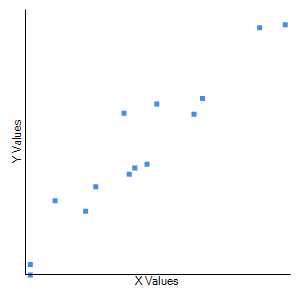
\includegraphics[scale=0.6]{Picture/One/TPvsTPFT.png}
 \caption{Throughput and throughput feature} 
 \label{fig:a:1}
  \end{subfigure}
  \begin{subfigure}[b]{0.5\textwidth}
    \center
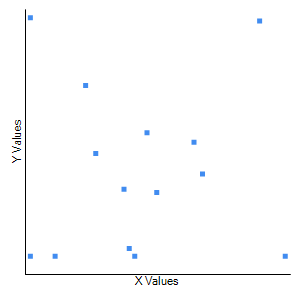
\includegraphics[scale=0.6]{Picture/One/TPvsTPB.png}
 \caption{Throughput and throughput bugs} 
\label{fig:b:1}
  \end{subfigure}
\caption{Correlation graphs between throughput (X-axis) and the throughput sub variables (Y-axis) for team one.}
\label{corr:Difference:1}
\end{figure}

\textbf{Team two's} \textit{throughput feature} differ from \textit{throughput} based on the correlation values from the \textit{bugs} correlation Table \ref{corr:bug}. One could believe the reason is because \textit{throughput bug} consists of 2/3 of \textit{throughput's} (460/690) dates, as shown in the descriptive statistic Tables \ref{DS:Throughput:2} and \ref{DS:TPB:2}. But the two tables and Table \ref{DS:TPFT:2} show that the total mean of \textit{throughput} is 4.4, while for \textit{throughput bug} it is 4.8 and 3.7 for \textit{throughput feature}. These three variables are quiet close, which could reflect that these three variables could be close based on correlation measurement. 
But, the correlation graphs in Figure \ref{corr:Difference:2} and the throughput correlation table in Section \ref{sec:corr:TP} shows otherwise. The Figure \ref{fig:b:2} shows a significant positive correlation, while Figure \ref{fig:a:2} shows dots that are more randomly placed. The throughput correlation Table \ref{corr:TP} represents the same result with a value of 0.97 for \textit{throughput bug} and  0.1 for \textit{throughput feature}.
\begin{figure}[h] 
  \begin{subfigure}[b]{0.5\textwidth}
  \center
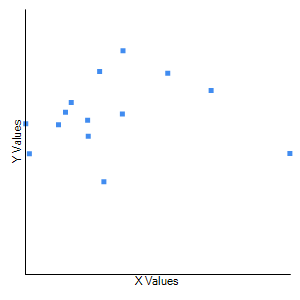
\includegraphics[scale=0.6]{Picture/Two/TPvsTPFT.png}
 \caption{Throughput and throughput feature} 
 \label{fig:a:2}
  \end{subfigure}
  \begin{subfigure}[b]{0.5\textwidth}
  \center
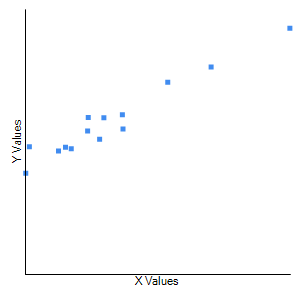
\includegraphics[scale=0.6]{Picture/Two/TPvsTPB.png}
 \caption{Throughput and throughput bug} 
\label{fig:b:2}
  \end{subfigure}
  \caption{Correlation graphs between throughput (X-axis) and the sub variables (Y-axis) for team two.}
\label{corr:Difference:2}
\end{figure}
\newpage


\textbf{Team three} has the correlation values of 0.52 for \textit{throughput bug}, 0.57 for \textit{throughput}  and 0.71 for \textit{throughput feature}, showed in WIP correlation Table \ref{corr:WIP:V2}. With these correlation values, it looks like \textit{throughput bug} represents most of the \textit{throughput} variable. The descriptive statistic tables empower the assumption. \textit{Throughput} contains 542 dates and has a total mean value of 3.7. \textit{Throughput feature} represents 200 of these dates and has a mean value of 3.3, while \textit{throughput bug} represents the remaining 342 dates and has a total mean value of 4,  shown in tables \ref{DS:Throughput:3}, \ref{DS:TPFT:3} and \ref{DS:TPB:3}. The \textit{throughput} correlation Table \ref{corr:TP:V2} shows both sub variables contribute, but \textit{throughput bug} contribute a little more with a correlation value of 0.98, while \textit{throughput feature}  has a correlation value of 0.90.



\textbf{Team four} has the correlation values 0.86 for \textit{throughput}, 0.85 for \textit{throughput feature}  and 0.27 for \textit{throughput bug}, showed in WIP correlation Table \ref{corr:WIP:V2}. These values indicate that \textit{throughput feature} represents the majority of \textit{throughput}. The dates in the descriptive statistic Tables \ref{DS:TP:4}, \ref{DS:TPFT:4} and \ref{DS:TPB:4} empower this assumption. The dates show that \textit{throughput} consists of 674 dates of which \textit{throughput feature} represents 644 and \textit{throughput bug} represents 30. The mean values on the other hand are 6.2 for \textit{throughput}, 6.2 for \textit{throughput feature} and 5.6 for \textit{throughput bug}. The mean values indicate that \textit{throughput feature} represents the most of \textit{throughput}, but \textit{throughput bug} contributes. The correlation graphs in Figure \ref{corr:Difference:4} and the correlation values of 1 for \textit{throughput feature} and 0.32 for \textit{throughput bug} showed by \textit{throughput} correlation Table \ref{corr:TP:V2} show otherwise. The correlation table and the graphs show  \textit{throughput feature} represents most of the \textit{throughput} variable.

\begin{figure}[h] 
  \begin{subfigure}[b]{0.5\textwidth}
  \center
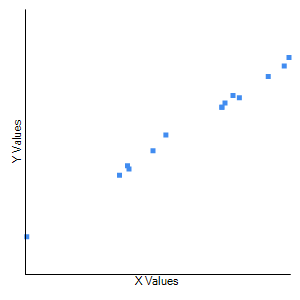
\includegraphics[scale=0.6]{Picture/Four/TPvsTPFT.png}
 \caption{Throughput and throughput feature} 
 \label{fig:a:4}
  \end{subfigure}
  \begin{subfigure}[b]{0.5\textwidth}
  \center
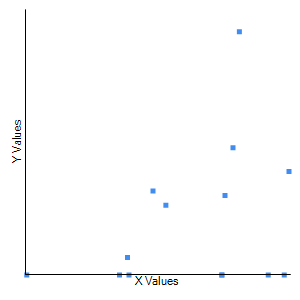
\includegraphics[scale=0.6]{Picture/Four/TPvsTPB.png}
 \caption{Throughput and throughput bug} 
\label{fig:b:4}
  \end{subfigure}
  \caption{Correlation graphs between throughput (X-axis) and the sub variables (Y-axis) for team four.}
\label{corr:Difference:4}
\end{figure}
\newpage


\textbf{Team five} has a significant correlation for \textit{throughput bug} with a value of 0.54, \textit{throughput} with a value of 0.52, but not \textit{throughput feature}. \textit{Throughput feature} has a correlation value of 0.25, as showed in WIP correlation Table \ref{corr:WIP}. Based on these values, one can assume that \textit{throughput bug} represents most of \textit{throughput} for team five. The descriptive statistic Tables \ref{DS:Throughput:5}, \ref{DS:TPFT:5} and \ref{DS:TPB:5} show \textit{throughput} consist of 657 dates. Out of the 657 dates, represents \textit{throughput feature} 108 dates, and \textit{throughput bug} 556 dates. These values also point towards the fact that \textit{throughput bug} represents most of \textit{throughput}. The overall mean for \textit{throughput} is 6.3, for \textit{throughput feature} it is 5.7 and for \textit{throughput bug} it is 6.4. Based on these values, it looks like both the sub variables contribute. The throughput correlation Table \ref{corr:TP} proves with the values 0.85 for \textit{throughput feature} and 0.99 for \textit{throughput bug} that both the sub variables contribute, but \textit{throughput bug} contribute most.



\textbf{Team six} has significant correlation to \textit{throughput} and \textit{throughput feature} showed in WIP correlation Table \ref{corr:WIP}, while \textit{throughput bug} does not. \textit{Throughput}, \textit{throughput feature} and \textit{throughput bug} has the correlation values 0.64, 0.68 and 0.07. Based on these values, one can assume \textit{throughput feature} contribute a greater proportion to \textit{throughput} than \textit{throughput bug}. The total row in Tables \ref{DS:Throughput:6},  \ref{DS:TPFT:6} and \ref{DS:TPB:6} show \textit{throughput feature} consist of 609 dates and has a mean value of 4.8, while \textit{throughput bug} consist of 82 dates  and a mean value of 3.3. \textit{Throughput} consists of 691 dates and has a mean value of 4.58. With the mean values and the number of dates, the assumption of \textit{throughput feature} represents more of \textit{throughput} than \textit{throughput bug} is empowered. The throughput correlation Table \ref{corr:TP} proves the assumption with a \textit{throughput feature}  correlation value of 0.99 and \textit{throughput bugs}  value of 0.04. 

\textbf{Team seven} has a significant correlation value for \textit{throughput}, \textit{throughput feature}, but not \textit{throughput bug}, as showed in WIP correlation Table \ref{corr:WIP}. The table showed a correlation value of 0.67 for \textit{throughput}, 0.63 for \textit{throughput feature} and 0.55 for \textit{throughput bug}. The difference between the correlation values is small, which also can be assumed by the total row in Tables \ref{DS:Throughput:7},  \ref{DS:TPFT:7} and \ref{DS:TPB:7}. The total rows show \textit{throughput} has a mean of 2.7, while \textit{throughput feature} has a mean value of 2.8 and \textit{throughput bug} has a mean value of 2.6. \textit{Throughput feature} contributes 156 dates to \textit{throughput} and \textit{throughput bug} contributes 172 dates. Based on these numbers, it looks like both the sub variables contribute. The \textit{throughput} correlation table in Section \ref{sec:corr:TP} proves the assumption with values of .91 for both \textit{throughput feature} and \textit{bug}.  

\textbf{Team eight} has a significant correlation value for \textit{throughput bug}, but not \textit{throughput}, as showed in bugs correlation Table \ref{corr:bug}. The descriptive statistic Tables \ref{DS:Throughput:8}, \ref{DS:TPFT:8} and \ref{DS:TPB:8} show \textit{throughput bug} consist of 99 dates and has a total mean of 1.5 while \textit{throughput feature} consist of 92 dates and a total mean of 3.2 and \textit{throughput} has mean of 2.3 and contains 191 dates.  On the basis of these numbers it will look like both of the sub variables of \textit{throughput} contributes and both of them should have close relationship to \textit{throughput}.  The correlation graphs in Figure \ref{corr:Difference:8} shows otherwise. The Figure \ref{fig:a:8} shows dots in an upward direction, hence positive correlation, while in Figure \ref{fig:b:8} almost all the dots are all gathered around the low values of Y. The Figures in \ref{corr:Difference:8} reflects the correlation value 0.94 for \textit{throughput feature} and 0.44 for \textit{throughput bug}.

\begin{minipage}[t]{\linewidth}
\begin{figure}[H] 
  \begin{subfigure}[b]{0.5\textwidth}
  \center
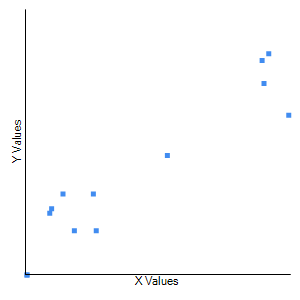
\includegraphics[scale=0.6]{Picture/Eight/TPvsTPFT.png}
 \caption{Throughput and throughput feature} 
 \label{fig:a:8}
  \end{subfigure}
  \begin{subfigure}[b]{0.5\textwidth}
  \center
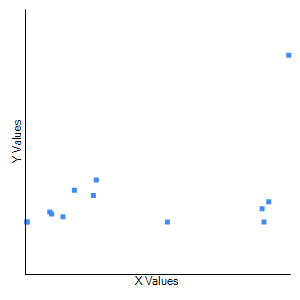
\includegraphics[scale=0.6]{Picture/Eight/TPvsTPB.png}
 \caption{Throughput and throughput bug} 
\label{fig:b:8}
  \end{subfigure}
  \caption{Correlation graphs between throughput (X-axis) and the sub variables (Y-axis) for team eight.}
\label{corr:Difference:8}
\end{figure}
\end{minipage}


\textbf{Team nine} has a significant positive correlation for \textit{throughput} and \textit{throughput bug}. The reason \textit{throughput feature} does not has a significant correlation while \textit{throughput} has it, in respect of the bugs correlation Table \ref{corr:Bugs:v2}, could be because \textit{throughput bug} represents most of the \textit{throughput} variable, as shown in Tables \ref{DS:Throughput:9}, \ref{DS:TPFT:9} and \ref{DS:TPB:9}. The \textit{throughput} variable contains 521 dates and has a mean value of 2.6. \textit{Throughput feature} represents 214 of these dates and has a total mean of 2.4, while \textit{throughput bug} represents the remaining 307 dates and has a total mean of 2.8. These variables indicate that both the \textit{throughput} sub variables contribute. The throughput correlation Table \ref{corr:TP:V2} proves that both the attributes contributes, but \textit{throughput bug} contributes the most with a correlation value of 0.95, while \textit{throughput feature} has a correlation value of 0.82. 


\textbf{Team ten} has significant positive relationship for \textit{throughput} and \textit{throughput bug}, but not for \textit{throughput feature}, as showed in WIP correlation Table \ref{corr:WIP}. \textit{Throughput} for team ten consists of 404 dates as showed in the total row in Table \ref{DS:Throughput:7}. \textit{Throughput bug} represents 335 of these dates, while \textit{throughput feature} represents the remaining 69 dates as shown in Tables \ref{DS:TPFT:7} and \ref{DS:TPB:7}. But the overall mean for \textit{throughput}, \textit{throughput feature} and \textit{throughput bug} is 2.2, 2.3 and 2.2, which could reflect a close relationship between these three variables. The throughput correlation table in Section \ref{sec:corr:TP} and the correlation graphs in Figure \ref{corr:Difference:10} disproves that assumption. The Figure \ref{fig:a:WIP:10} shows a vague significant positive correlation, while Figure \ref{fig:b:WIP:10} shows a significant positive correlation. The correlation table shows  \textit{throughput bug} with a correlation of 0.98 and \textit{throughput feature} with a correlation of 0.43.  Which proves that \textit{throughput bug} represents most of \textit{throughput}. 

\begin{figure}[h] 
  \begin{subfigure}[b]{0.5\textwidth}
  \center
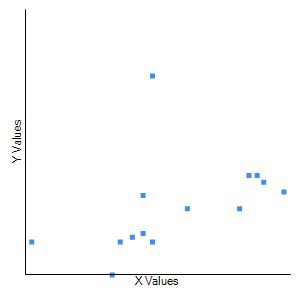
\includegraphics[scale=0.6]{Picture/Ten/TPvsTPFT.png}
 \caption{Throughput and throughput feature} 
 \label{fig:a:WIP:10}
  \end{subfigure}
  \begin{subfigure}[b]{0.5\textwidth}
  \center
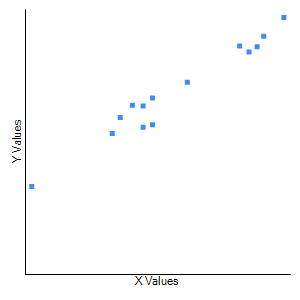
\includegraphics[scale=0.6]{Picture/Ten/TPvsTPB.png}
 \caption{Throughput and throughput bug} 
\label{fig:b:WIP:10}
  \end{subfigure}
  \caption{Correlation graphs between throughput (X-axis) and the sub variables (Y-axis) for team ten.}
\label{corr:Difference:10}
\end{figure}

\subsection{Churn}
In WIP correlation Table \ref{corr:WIP} have the three churn variables for \textbf{team one} scattered correlation values. \textit{Churn} has a value of 0.47, \textit{churn feature} has a value of 0.72 and \textit{churn bug} of 0.15.  Judging from these variables, it will look both \textit{churn feature} and \textit{churn bug}  contribute to \textit{churn}. The descriptive statistic Tables \ref{DS:Churn:1}, A.4a and A.4b empower the assumption. The total mean of \textit{churn} is 20.2, while \textit{churn feature} has total mean of 24.5 and \textit{churn bug} has a total mean of 16.8. The descriptive statistic tables also shows that \textit{churn feature} contribute 150 dates to \textit{churn}, while \textit{churn bug} contribute 189 dates. The churn correlation table in Section \ref{sec:corr:churn} proves the assumption. Both \textit{churn feature} (0.57) and \textit{churn bug} (0.80) has a significant positive correlation to \textit{churn}. Judging from the correlation table from Section \ref{sec:corr:TP},  one can assume that correlation is not transitive. The paper "The Non-Transitivity of Pearson's Correlation Coefficient: An Educational Perspective" \parencite{corr:transitive} proves the assumption. 

\textit{Churn} and \textit{churn bug} has a significant negative correlation for \textbf{team two}. \textit{Churn feature} on the other hand has a correlation value of -0.25, showed in WIP correlation Table \ref{corr:WIP}. According to the correlation values, one can assume that \textit{churn bug} represents most of \textit{churn}. The Tables \ref{DS:Churn:2}, \ref{DS:CF:2} and \ref{DS:CB:2} empower the assumption. \textit{Churn bug} contribute 521 dates and has a total mean value of 36.3. \textit{Churn feature} contribute 257 dates and has a mean value of 100.6. The total churn contains 778 dates and has a total mean of 57.6. The \textit{churn} correlation table in Section \ref{sec:corr:churn} shows both the \textit{churn} variables contribute with a correlation value of 0.7 for \textit{churn bug} and 0.58 for \textit{churn feature}. 

The three \textit{churn} variables for \textbf{team three} have the correlation values of -0.45 for \textit{churn}, -0.27 for \textit{churn feature} and -0.64 for \textit{churn bug}, as showed in the correlation Table \ref{corr:lt}, for lead time. These values indicate more contribution from \textit{churn bug}  than \textit{churn feature}. The total dates and the mean from Tables \ref{DS:Churn:3}, \ref{DS:CF:3} and \ref{DS:CB:3} empower the assumption. The total \textit{churn} consists of 576 dates and a total mean of 61.8. \textit{Churn feature}  represents 205 of these dates and has a total mean of 98.9. \textit{Churn bug} answers for the remaining 371 dates and has a total mean of 41.4. The \textit{churn} correlation table in Section \ref{sec:corr:churn} proves the assumption. Still,  \textit{churn bug} has a correlation of 0.85, while the correlation value between \textit{churn feature} and \textit{churn} is 0.90. The strong relationship between \textit{churn} and \textit{churn bug} shows that total dates and total mean can be used as an indicator of the relationship between variables, but it can't state it.
%siden man kan anta utfra tabellene at churn bug ikke gir så mye til churn pga total mean andd total N


The \textit{churn} variable for \textbf{team four} has the correlation value of 0.97, \textit{churn feature} has the correlation value of 0.96 and  \textit{churn bug} has the correlation value of 0.2, as showed in the correlation Table for lead time, Table \ref{corr:lt}. The descriptive statistic Tables \ref{DS:Churn:4}, \ref{DS:CF:4} and \ref{DS:CB:4} shows that \textit{churn} consist of 574 dates. \textit{Churn bug} represents 78 of these dates and \textit{churn feature} represents the remaining 496 dates. \textit{Churn features} has the total mean of 8.4, \textit{churn bug's} mean is 1 and \textit{churn's} mean is 7.4. These variables clearly indicate the strong relationship between \textit{churn feature} and \textit{churn}. The churn correlation Table \ref{corr:churn} verifies the theory with \textit{churn feature} has the correlation value of 0.99 and \textit{churn bug} has the correlation value 0.13.

\textit{Churn bug} for \textbf{team five} has a significant positive correlation of .94, while \textit{churn feature} has the correlation value of 0.22, as shown in \textit{churn} correlation Table \ref{corr:churn}. This proves that \textit{churn bug} represents most of \textit{churn}. The Tables \ref{DS:Churn:5}, \ref{DS:CF:5} and \ref{DS:CB:5} show the same result. \textit{Churn} consists of 698 dates and has a total mean of 33.4, while \textit{churn feature} and \textit{churn bug} represents has 123 dates and 575 dates. The total mean of \textit{churn feature} is 52.1 and for \textit{churn bug} it is 29.4. 


\textbf{Team six} has a significant correlation value of 0.77 for \textit{churn bug}, while both \textit{churn} and \textit{churn feature} has the values of -0.30 and -0.36, showed in WIP correlation Table \ref{corr:WIP}. Based on these values, one can assume \textit{churn feature} represents most of \textit{churn}. The Tables \ref{DS:Churn:6}, \ref{DS:CF:6} and \ref{DS:CB:6} back this theory. The tables show \textit{churn feature} contribute 576 dates to \textit{churn} and has a total mean of 105.9. \textit{Churn bug} contains of 180 dates and has a total mean value of 73.8. \textit{Churn} has 756 dates and a total mean value of 98.3.  The churn correlation table in Section \ref{sec:corr:churn} proves the assumption of \textit{churn feature} represent most of \textit{churn}, with the correlation values 0.98 for  \textit{churn feature} and -0.02 for \textit{churn bug}.

\textit{Churn feature} for \textbf{team seven} has the correlation value of 0.91 while \textit{churn bug} has the correlation value 0.13, as showed in \textit{churn} correlation Table \ref{corr:churn}. The descriptive statistic Tables \ref{DS:Churn:7}, \ref{DS:CF:7} and \ref{DS:CB:7} shows that \textit{churn} contains 359 dates and has a total mean of 77.3.  \textit{Churn feature} represents 141 of these dates, and has a total mean of 121.2. \textit{Churn bug} represents the 218 remaining dates and has a total mean of 48.9. Based on these values, one could assume that both  \textit{churn feature} and  \textit{churn bug} contribute to  \textit{churn}, but the churn correlation table  and  the graphs in Figure \ref{corr:Difference:7} disapproves that. Which once again shows that the descriptive statistic tables can be used as indication of relationship, but cannot prove them.

\begin{minipage}[t]{\linewidth}
\begin{figure}[H]
  \begin{subfigure}[b]{0.5\textwidth}
  \center
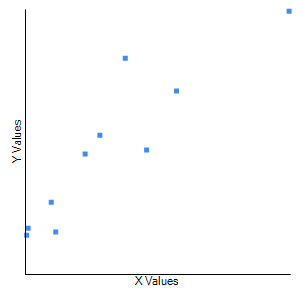
\includegraphics[scale=0.6]{Picture/Seven/ChrnvsChrnFT.png}
 \caption{Churn and churn feature} 
 \label{fig:a:7}
  \end{subfigure}
  \begin{subfigure}[b]{0.5\textwidth}
  \center
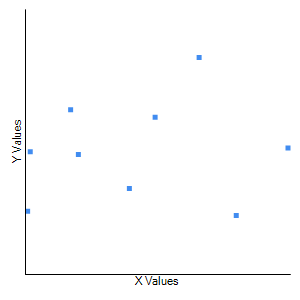
\includegraphics[scale=0.6]{Picture/Seven/ChrnvsChrnB.png}
 \caption{Churn and churn bug} 
\label{fig:b:7}
  \end{subfigure}
\caption{Correlation graphs between the churn (X-axis)  and the sub variables (Y-axis) for team seven.}
\label{corr:Difference:7}
\end{figure}
\end{minipage}

\textbf{Team eight} has a significant correlation to \textit{churn} and \textit{churn feature}, but not \textit{churn bug}, as showed in lead time's correlation Table  \ref{corr:lt}. The correlation values for \textit{churn} is 0.91, for \textit{churn bug} it is  -0.12 and for \textit{churn feature} it is 0.79. Based on these variables, it looks like \textit{churn feature} represents a greater part of the \textit{churn}. The Tables \ref{DS:Churn:8}, \ref{DS:CF:8} and \ref{DS:CB:8} indicate otherwise. \textit{Churn} is composed of 137 dates, and has a total mean of 13.4. \textit{Churn feature} represents 79 of these tasks and has a total mean of 17.4. \textit{Churn bug} represents the remaining 58 tasks and has a total mean of 8.  The values indicate both \textit{churn feature} and \textit{churn bug} contribute to \textit{churn}. The Figure \ref{corr:Difference:lt:8} and correlation Table \ref{corr:churn} disapproves the assumption. The \textit{churn} correlation Table \ref{corr:churn} shows that \textit{churn feature} has the correlation of 0.84, while \textit{churn bug} has the value of -0.1. This is the same as shown in the correlation graphs. The Figure \ref{fig:a:lt:8} shows a clear positive correlation, while Figure \ref{fig:b:lt:8} shows no pattern and shows a correlation close to 0. 
\begin{minipage}[t]{\linewidth}
\begin{figure}[H] 
  \begin{subfigure}[b]{0.5\textwidth}
  \center
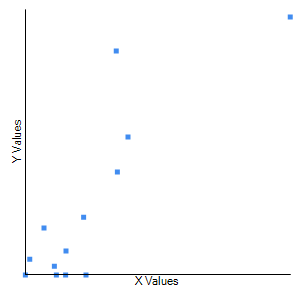
\includegraphics[scale=0.6]{Picture/Eight/ChurnVSChurnFT.png}
 \caption{Churn and churn feature} 
 \label{fig:a:lt:8}
  \end{subfigure}
  \begin{subfigure}[b]{0.5\textwidth}
    \center
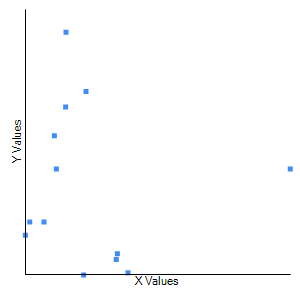
\includegraphics[scale=0.6]{Picture/Eight/ChurnVSChurnB.png}
 \caption{Churn and churn bug} 
\label{fig:b:lt:8}
  \end{subfigure}
\caption{Correlation graphs between the churn (X-axis)  and the sub variables (Y-axis) for team eight.}
\label{corr:Difference:lt:8}
\end{figure}
\end{minipage}

\textbf{Team nine} has a significant correlation value of -0.62 to \textit{churn feature}, while \textit{churn} has the value of -0.48 and \textit{churn bug} has the value -0.04, as showed in bugs correlation Table \ref{corr:bug}. Based on the correlation values, it looks like \textit{churn feature} represents most of \textit{churn}. The descriptive statistic data show otherwise. \textit{Churn} consists of 548 dates, \textit{churn feature} represents 201 of these dates and \textit{churn bug} represents the remaining 347 dates, as shown in Tables \ref{DS:Churn:9}, \ref{DS:CF:9} and \ref{DS:CB:9}.  The total mean of \textit{churn feature} is 115.9, the total mean for \textit{churn} is 72.2 and the total mean for \textit{churn bug} is 46.1. Judging from these numbers, both \textit{churn feature} and \textit{churn bug} contribute to \textit{churn}. In the graphs in Figure \ref{corr:Difference:9}, one can see Figure \ref{fig:a:9} show a positive correlation. The Figure \ref{fig:b:9} represents a positive correlation, but not as high as Figure \ref{fig:a:9}. The \textit{churn} correlation states the same,  Table \ref{corr:churn} shows \textit{churn feature} correlation values is 0.60 and \textit{churn bug} correlation value is 0.39. This proves that \textit{churn feature} represents most of \textit{churn}.

\begin{minipage}[t]{\linewidth}
\begin{figure}[H] 
  \begin{subfigure}[b]{0.5\textwidth}
    \center
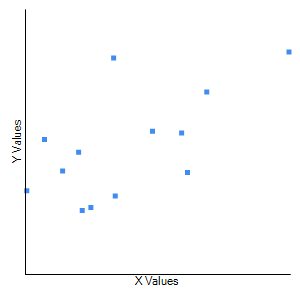
\includegraphics[scale=0.6]{Picture/Nine/ChurnVsChurnFT.png}
 \caption{Churn and churn feature} 
 \label{fig:a:9}
  \end{subfigure}
  \begin{subfigure}[b]{0.5\textwidth}
  \center
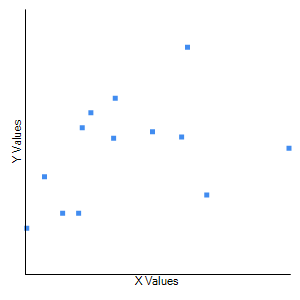
\includegraphics[scale=0.6]{Picture/Nine/ChurnVsChurnB.png}
 \caption{Churn and churn bug} 
\label{fig:b:9}
  \end{subfigure}
\caption{Correlation graphs between the churn (X-axis)  and the sub variables (Y-axis) for team nine.}
\label{corr:Difference:9}
\end{figure}
\end{minipage}

\textbf{Team ten} has a significant correlation value of 0.94 for \textit{churn bug} and \textit{churn feature} has the correlation value 0.14, as showed in \textit{churn} correlation Table \ref{corr:churn}. This shows that churn bug represents most of \textit{churn}.  Based on the Tables \ref{DS:Churn:10}, \ref{DS:CF:10} and \ref{DS:CB:10}, one can see that \textit{churn} contains 361 dates and has a total mean value of 45.4. \textit{Churn feature} represents 69 of these dates and has a total mean of 75.5, while \textit{churn bug} represents 292 of \textit{churn's} dates and has a total mean of 38.3. These data also shows the relationship between \textit{churn} and \textit{churn bug}.  

\section{WIP and throughput} 
\vspace{-0.5em}
In this work, throughput is a measure to see how productive teams are. In Section \ref{WIPsec}, there was stated by various people, when lowering WIP-limit the \textit{throughput} increases. The paper "Studying Lean-Kanban Approach Using Software Process Simulation" \parencite{DavidAnderson} simulated a  lean-kanban process, as stated in \ref{WIPsec}. The simulation showed when WIP was limit; the software process used 100 days and 120 days when WIP was not limit. The paper "Simulation of software maintenance process, with and without a work-in-process limit" \parencite{SMR:SMR1599} showed that WIP-limit could lead to improvement in throughput. The paper also showed that when taking a process without WIP-limit, and simulate it using WIP-limit it outperformed the process without WIP-limit.


The Tables \ref{DS:corr:TP} and \ref{DS:corr:TP:v2} from this result show no evidence towards the fact that lowering WIP-limit will increase \textit{throughput}. \textit{Throughput} has the average correlation value of 0.6 when team size is \textbf{not} taken into account and 0.4 otherwise. One can argue that the throughput correlation value is biased when team size is \textbf{not} taken into account, based on the strong team size correlation. But the Table \ref{DS:corr:TP:v2}, where team size is taken into account shows an average correlation value of 0.4 between \textit{throughput} and \textit{WIP} when team size is taken into account.

When team size is \textbf{not} taken into account,  all of the teams have a positive correlation between \textit{WIP} and \textit{throughput}, and seven of the teams have a significant correlation value, shown in Table \ref{corr:WIP}.  When team size is taken into account the Table \ref{DS:corr:WIP:v2}  shows nine out of ten teams have a positive correlation between \textit{WIP} and \textit{throughput}. Team ten is the only team with a negative correlation.  Team five, six, eight and ten has a low correlation value, team one and seven has a low-medium correlation value and team two, three, four and nine has a significant correlation relationship. The median between the teams when team size is \textbf{not} taking into account is 0.7 and 0.4 otherwise. The standard deviation is 0.2 when team size is \textbf{not} taking into account and 0.3 otherwise, shown by Tables \ref{DS:corr:WIP} and \ref{DS:corr:WIP:v2}. The median and standard deviation when team size is \textbf{not} taken into account shows most of the teams have a strong linear relationship between \textit{WIP} and \textit{throughput}. The median and standard deviation when team size is taken into account shows that more than half of the teams have at least  a medium correlation relationship.

The combined Table \ref{corr:All} shows a significant correlation value of 0.41 when team size is \textbf{not} taking into account, while Table \ref{corr:All:V2} shows an overall correlation of 0.05 when team size is taken into account. The values presented in this section point towards the fact that when \textit{WIP} increases, so does \textit{throughput}.


%The \textit{throughput} values show that when team size is \textbf{not} taking into account, seven of the ten teams have a significant linear relationship and the average \textit{throughput} value is 0.6. When team size is taken into account, four of the teams have a significant correlation and the average mean is 0.4. These values shows that \textit{throughput} has a positive correlation relationship with \textit{WIP}. The two median numbers shows at least 50\% of the correlation values have a medium-strong correlation value. The standard deviation shows a low-medium spread between the values, which indicates that the values are in the same range. The overall correlation value when team size is \textbf{not} taking into account shows a positive medium-strong linear relationship, but when team size is taken into consideration the overall linear relationship is 0.05, but the average for teams is 0.4 and four out of ten teams has a significant value.  Based on this, there is a low-medium linear relationship between \textit{WIP} and \textit{throughput}. 

%The two tables also show the sub variables of \textit{throughput} with a mean of 0.5 when team size is \textbf{not} taken into account and 0.3 otherwise. This display that both the sub variables  



Despite the relationship between \textit{WIP} and \textit{throughput}, the \textit{throughput} correlation Table \ref{DS:corr:TP:v2} in Section \ref{sec:corr:TP} shows that \textit{throughput bug} has a mean correlation value of 0.8, \textit{bugs} and \textit{throughput feature} has an average correlation value of 0.6 and  \textit{lead time} has the average value of 0.5.
The combine Table \ref{corr:All:V2} shows \textit{throughput} has significant correlation values to all variables except \textit{WIP} and \textit{churn feature}, when team size is taken into account.

When team size is \textbf{not} taken into account the Table \ref{DS:corr:TP} shows that \textit{throughput feature} has a mean correlation value of 0.8, \textit{throughput bug} has an average value of 0.7, \textit{bugs} and \textit{WIP} has a value of 0.6 and both \textit{lead time} and \textit{team size} has an average correlation value of 0.5. The combined Table \ref{corr:All} shows \textit{throughput} has a significant correlation relationship to all variables except \textit{WIP} and \textit{churn feature}. 

The \textit{throughput's} correlation values are isolated and can only be used to see what impact \textit{throughput} has on a software process. One cannot say if \textit{WIP} decreases, then \textit{throughput} decreases and then all the variables with a significant positive correlation to \textit{throughput} decreases. The \textit{throughput} correlation values also shows the \textit{WIP} relationship decreases when \textit{team size} is taken into account, but the relationship between the other variables do not differ in the same extent.




\section{WIP and lead time}
\vspace{-1em}
As stated in Section \ref{sec:in:lt}, lead time could be used to track how quickly software is delivered to customers. Each development process would like to get their lead time as low as possible. In Section \ref{WIPsec} there is stated that WIP-limits are important to reduce lead times. The result from this work when team size was \textbf{not} taken into account shows mean correlation relationship of 0.5 between \textit{WIP} and \textit{lead time} across the teams,  as shown in Table \ref{DS:corr:WIP}.  The correlation Table \ref{corr:WIP} shows Team one, four, five, seven and ten has significant positive correlation relationship and both team two and three has a medium correlation relationship.

The result from when team size was taken into account shows an average correlation relationship of 0.2, which is a weaker correlation relationship than when team size was \textbf{not} taken into account. Three of the ten teams have a significant positive correlation, while the rest of teams' correlation values vary from -0.18 to 0.32, as shown by Tables \ref{corr:WIP:V2} and \ref{DS:corr:WIP:v2}. 

The standard deviation shows a variation of 0.2 and a median of 0.5 when team is \textbf{not} taken into account. The standard deviation when team size is taken into account is 0.4 and the median is 0, as shown in Tables  \ref{DS:corr:WIP} and \ref{DS:corr:WIP:v2}. The standard deviation shows a high proliferation of values when team size is taken into account. The standard deviation shows evidence of spread relationship between \textit{WIP} and \textit{lead time} across the teams  when team size is taken into account.   The standard deviation value of 0.2 shows that  each of the ten \textit{lead time} values are closer to each other when team size is \textbf{not} taken into account.  

The combine correlation Table \ref{corr:All} shows that all teams combined have a significant correlation value of 0.27, when team size is \textbf{not} taken into account.  The correlation Table \ref{corr:All:V2} shows a non-significant correlation value of 0.05 when team size is taken into account. The value presented in this section shows when time size is taken into account, there is no linear relationship between \textit{WIP} and \textit{lead time}. When team size is \textbf{not} taken into account; there is a low significant correlation value for all the teams combined and medium-strong positive correlation when each team is measured independently. Either way, based on these results, there is no evidence showing that WIP-limit will decrease \textit{lead time}.


Despite the relationship between \textit{WIP} and \textit{lead time},  \textit{lead time} has a close positive relationship to four of the five individual variables, shown in Table \ref{DS:corr:LT:v2}. \textit{Throughput, throughput bug}, \textit{bugs} and  \textit{bugs finished, quarter}  has the average correlation value 0.5, while \textit{churn} has the value of 0.4, when team size is taken into account. When team size is \textbf{not} taken into account, \textit{WIP} and \textit{throughput} has an average correlation value of 0.5 and \textit{throughput feature} has the value 0.4, while the rest variables has a value of $\pm$ 0.3 or less. The combine Table \ref{corr:All} shows an overall significant positive correlation between \textit{lead time} and both \textit{team size} and \textit{WIP}, when team size is \textbf{not} taken into account. When team size is taken into account \textit{throughput}, \textit{throughput bug}, \textit{bugs}, \textit{bugs finished quarter}, \textit{avg days in backlog, bugs}, \textit{churn} and \textit{churn feature} has a significant positive correlation, as shown by Table \ref{corr:All:V2}. These values show the impact \textit{lead time} has on a development process.  The significant correlation value and the high average correlation value between \textit{lead time} and \textit{throughput} is odd, these values should be further investigated. 

\section{WIP and bugs}
To minimize bugs should be a goal independent of software process and methods. If WIP-limit could reduce bugs without compromising, one could conclude that WIP-limit matter in software development. The paper cited by Shinkle stated; when WIP was too high, the number of bugs increased  \parencite{Shinkle}.

The result from this work shows when team size is \textbf{not} taken into account, the average correlation value between \textit{WIP} and \textit{bugs} is 0.4 and four of the teams have a significant positive correlation value between \textit{bugs} and \textit{WIP}. All ten teams have a positive correlation value, as shown in Table \ref{corr:WIP}. The two variable \textit{bug finished, quarter} and \textit{avg days backlog bugs} is used as a side measure to how long bugs are in backlog and the amount of bugs fixed vs. the amount of bugs recorded in system per quarter. The average correlation value between \textit{WIP} and both \textit{bug finished, quarter} is 0.3 and \textit{avg days backlog, bugs} is 0.1. The value \textit{bug finished, quarter} shows a low-medium average correlation relationship. The mean correlation value of 0.1   for  \textit{avg days backlog bugs}, the combine correlation value of 0.17 from Table \ref{corr:All} and the fact that there is one team with a significant correlation relationship between \textit{avg days backlog, bugs} and \textit{WIP} shows that  \textit{WIP} limit has no influence on the number of days bugs are in backlog, when \textit{team size} is \textbf{not} taken into account. The \textit{bugs finished, quarter} with the mean of 0.3, also has a significant positive correlation of 0.17. These values show weak correlation relationship between \textit{bugs finished, quarter} and \textit{WIP}. 

When team size is taken into account, the average correlation value is 0.2 for \textit{bugs}, as shown by Table \ref{DS:corr:WIP:v2}.  Eight out of ten teams have a positive correlation relationship, but only one team has a significant positive value. The  \textit{bug finished, quarter} and \textit{avg days backlog, bugs}  has the average correlation values 0.2 and -0.1. For \textit{bug finished, quarter} are there four teams with a positive significant correlation and one team with a negative. For \textit{avg days backlog, bugs} is there one team with a negative significant correlation. The combine Table \ref{corr:All:V2} shows \textit{bugs finished, quarter} with a significant correlation value of -0.20 and \textit{avg days in backlog, bugs} with a negative correlation value of -0.08.

The standard deviation when team size is \textbf{not} taken into account is 0.2 and the median is 0.5. The median when team size is taken into account is 0.2 and the standard deviation is increased is 0.3. The median numbers shows significant impact of team size between the relationship of \textit{WIP} and \textit{bug}. The standard deviation values for the two cases shows a minor variation between the two results variables, shown in \ref{DS:corr:WIP} and \ref{DS:corr:WIP:v2}    

When team size is \textbf{not} taken into account, the overall correlation value is significant with a value of  0.41, shown in Table \ref{corr:All}.  The correlation Table \ref{corr:All:V2} shows the correlation values from when time size is taken into account. The table shows an overall correlation value of 0.12. The values from this section shows there is no evidence of that WIP-limit helps increase or decrease bugs when \textit{team size} is taken into account, but without \textit{team size} taken into account, \textit{WIP} and \textit{bugs} has a positive significant correlation relationship.  


The \textit{bug} correlation tables in Section  \ref{sec:corr:bug} shows the \textit{bugs} variable has a average correlation of 0.6 to \textit{throughput} and a correlation value of 0.3 to \textit{bugs finished, quarter} \textit{avg days backlog, bugs}, \textit{lead time} and \textit{team size}, when time size is \textbf{not} taken into account. When team size is taken into account, \textit{bugs} has a average correlation value of 0.6 to \textit{throughput} again, \textit{bugs finished quarter} has the average correlation value 0.5, \textit{avg days in backlog, bugs} has the average value of 0.4, \textit{lead time} 0.5 and \textit{churn} 0.3. When team size is taken into account, the correlation relationship between the variables and \textit{bugs} increases for almost each variable.
 

\section{WIP and Churn}
Churn is used as surrogates for effort in this work. Based on the descriptive statistics tables, independently of  team size; there is no relationship between \textit{WIP} and \textit{churn} or the sub variables of churn according to Tables \ref{DS:corr:WIP} and \ref{DS:corr:WIP:v2}. The results show respectively an average correlation of -0.1 and 0. When team size is \textbf{not} taken into account, two of the teams have a significant correlation, one of them has a positive correlation and the other has a negative. When team size is taken into account, there is one team with a significant positive correlation value.

The standard deviation for both the results are 0.4, while the median is 0.1 when team size is \textbf{not} taken into account and -0.1 for the other case. The standard deviation empowers the assumption of a relationship between \textit{churn} and \textit{WIP}, because the values are spread and there is no pattern.  The Table \ref{corr:All} shows an overall correlation value of 0.06 when team size is taken into account. The Table \ref{corr:All:V2} shows a correlation value of -0.07. These values show that WIP-limit has no impact on \textit{churn}.

Section \ref{sec:corr:churn} show \textit{churn} correlation tables. The Table \ref{DS:corr:Churn} shows when team size is \textbf{not} taken into account, \textit{churn} has no correlation relationship between any of the other variables, except the \textit{churn's} sub variables. When  team size is taken into account, \textit{bugs finished, quarter} has a strong average relationship with a value of 0.6, while \textit{lead time} has a value of 0.4, as shown by Table \ref{DS:corr:churn:v2}. The combine Table \ref{corr:All} shows \textit{churn} has a significant positive correlation value to both the sub variables and a significant negative correlation to \textit{team size}. When team size is taken into account, \textit{churn} has a significant positive correlation to \textit{throughput}, \textit{throughput bug}, \textit{bugs}, \textit{bugs finished, quarter}, \textit{avg days in backlog, bugs}, \textit{lead time} and \textit{churn bug}. 


\section{Team size}
As the different results sections in Chapter \ref{ch:res} and the sections above states, it is important to take team size into account when a case study like this is conducted. If team size were left out as a variable in this case study, \textit{WIP} would have an average correlation relationship of 0.6 with \textit{throughput} and 0.5 with \textit{bugs} and \textit{lead time}. These three correlation values decreased by 0.2  and 0.3 compared to when  team size was taken into account. The combine correlation Table  \ref{corr:All} shows that seven of the variables have a significant positive correlation with \textit{team size}. The table also shows eight out of eleven variables has a significant correlation value with \textit{WIP}, while Table \ref{corr:All:V2} shows one out of ten variables has a significant relationship. If team size were not taken into account the result from this work would have been biased. 


\iffalse
When time size was \textbf{not} taken into account for the \textit{throughput} variable, \textit{bugs} has a value of 0.6 and \textit{lead time} has a value of 0.5, which indicates a medium - strong relationship. The median in \textit{bugs} case is 0.8 and for \textit{lead time} it is 0.5 as shown in Tables \ref{DS:corr:TP} and \ref{DS:corr:TP:v2}. When team size is taken into account, the correlation values between \textit{throughput} and both \textit{bugs} and \textit{lead time} is the same, the standard deviation and median for \textit{bugs} is different.  If \textit{WIP} omitted, the correlation relationship between the other variables and \textit{throughput} does not differ to much.

The \textit{bugs} correlation tables \ref{DS:corr:Bugs} and \ref{DS:corr:Bugs:v2} shows a difference in the correlation value between \textit{bugs} and \textit{WIP}. The correlation value is increased by 0.2 when team size is \textbf{not} taken into account. Both the \textit{throughput} correlation values are 0.6. The correlation value for \textit{lead time} is also increased by 0.2 when team size is \textbf{not} taken into account, while churn increased by 0.3. These values show an impact of team size on the correlation relationship for 3 of 4 variables. For \textit{lead time} increases the churn value by 0.2 when time size is \textbf{not} taken into account, otherwise are the correlation values for \textit{lead time} stated preceding paragraphs. 
\fi



\chapter{Conclusion}
\label{ch:conc}
In this work the main goal was to investigate the research question "Does WIP-limit in software development matter?" If so, "how can one find the optimal WIP-limit" and "Which parameters should be considered in order to optimize WIP-limits".  To answer the research questions a data set from a company called Software Innovation was interpreted. The data set is based on metadata about tasks from 2010 to 2013.

In light of the previous findings, the results from when team size was \textbf{not} taken into account are discarded. Because the data showed team size had a great impact on the correlation tables, which produced biased results.


If WIP-limit matters in software development some of its benefits should be to reduce bugs, increase throughput, decrease lead time etc. Based on the results from this work, \textit{WIP} has a positive medium mean relationship with \textit{throughput} on team level. On company level has \textit{WIP} and \textit{throughput} no linear relationship. The previous research has stated to lower WIP to decrease throughput, which this case study disapproves. On company level there was one significant correlation. There is also stated that WIP-limits decreases \textit{lead time}, the mean correlation value between these two variables is 0.2 and the overall correlation value between these two is 0.05. This shows evidence towards the fact that WIP-limit does not decrease \textit{lead time}. There is also stated that WIP-limit decreases number of \textit{bugs}. The mean correlation value between \textit{bugs} and \textit{WIP} is 0.2 and the overall correlation value is 0.12, which shows that WIP-limit does not decrease \textit{bugs}.  \textit{WIP} had one significant correlation, the significant correlation value was a negative one for \textit{bugs finished, quarter}. Because WIP-limits do not matter in software development based on this work, one cannot use these results to find an optimal WIP-limit or know which parameters to take into account in order to optimize WIP.

However, the results from this paper show some other findings. The importance of taking team size into account when measuring a similar research, the churn variable has no or little impact on the software process and the great impact the variables \textit{lead time}, \textit{bugs} and \textit{throughput} has in a software process. 
%The values of this data, example lead time has a close relationship between order empower this validity of this study

\section{Future work}
The conclusion from this work is made on one case study. I would recommend doing the same calculation as in this work with another data set and comparing the outcome. I would also suggest a different approach as looking more deeply into the relationship between \textit{WIP} and  \textit{team size}. I suggest one measure the number of employees working on each task instead of take the number of employees per quarter and divide on the mean of each variables value.

I will also suggest looking at the values up against release dates. The number of WIP's, throughput, bugs et cetera usually increase around release date, which could cause bias in the data. There is also done another research on the data from SI, I would suggest comparing the result from this work against the other research.


%%%%%%%%%%%%%%%%%%%%%%%% appendices %%%%%%%%%%%%%%%%%%% 
\begin{appendices}
\chapter{Descriptive statistics (DS) for the ten teams}
\label{app:DS}
The following tables show the descriptive statistics for the ten teams before team size was taken into account.
\section{Team 1 - Descriptive Statistics}
\begin{table}[!htbp]
\begin{adjustwidth}{-1.5cm}{}
 \begin{subfigure}[b]{0.7\textwidth}
 \scalebox{0.85}{
  \begin{tabular}{ | l | r | r | r | r | r | r | }
 \hline
 \textbf{Quarter} &	\textbf{N} &	\textbf{Mean} &	\textbf{Median} & \textbf{Std.Dev} & \textbf{Max}	& \textbf{Min} \\ \hline
 2010-3   & 25 & 3.6 & 4 & 0.6 & 5 & 3 \\ \hline
 2010-4  & 92 & 0.7 & 1 & 0.7 & 3 & 0\\ \hline
 2011-1  & 90 & 3.4 & 1 & 6.9 & 30 & 0\\ \hline
 2011-2  & 91 & 13.2 & 4 & 14.5 & 51 & 2 \\ \hline
 2011-3  & 92 & 1.8 & 2 & 0.6 & 3 & 1 \\ \hline
 2011-4  & 92 & 14.3 & 4 & 22.7 & 97 & 1 \\ \hline
 2012-1  & 91 & 22.2 & 21 & 14.5 & 67 & 4 \\ \hline
 2012-2  & 91 & 30.3 & 23 & 29 & 107 & 9 \\ \hline
 2012-3  & 92 & 36 & 38.5 & 13.6 & 65 & 18 \\ \hline
 2012-4  & 92 & 34.7 & 28.5 & 16.9 & 99 & 25 \\ \hline
 2013-1  & 90 & 32.8 & 25 & 13.7 & 85 & 25 \\ \hline
 2013-2  & 91 & 67.1 & 54 & 44.3 & 178 & 3 \\ \hline
 2013-3  & 92 & 7.4 & 3 & 8.8 & 31 & 1 \\ \hline
 2013-4  & 76 & 5 & 1 & 8.1 & 35 & 1 \\ \hline
 Total  & 1197 & 20.5 & 12 & 26.2 & 178 & 0\\ \hline
\end{tabular}
}
\caption{DS - WIP} 
\label{DS:WIP:1}
\end{subfigure}
\begin{subfigure}[b]{0.3\textwidth}
 \scalebox{0.85}{
 \begin{tabular}{ | l | r | r | r | r | r | r | }
 \hline
 \textbf{Quarter} &	\textbf{N} &	\textbf{Mean} &	\textbf{Median} & \textbf{Std.Dev} & \textbf{Max}	& \textbf{Min} \\ \hline
 2010-3   & 3 & 3 & 1 & 3.5 & 7 & 1 \\ \hline
 2010-4  & 3 & 1 & 1 & 0 &1 & 1 \\ \hline
 2011-1  & 7 & 10.4 & 11 & 8.1 & 25 & 1 \\ \hline
 2011-2  & 32 & 9.4 & 10 & 6.7 & 26 & 1 \\ \hline
 2011-3  & 2 & 1 & 1 & 0 &1 & 1 \\ \hline
 2011-4  & 25 & 14.9 & 10 & 14.6 & 49 & 1 \\ \hline
 2012-1  & 49 & 8.6 & 5 & 8.1 & 33 & 1 \\ \hline
 2012-2  & 45 & 11.2 & 3 & 16 & 56 & 1 \\ \hline
 2012-3  & 34 & 5.5 & 3 & 6.3 & 23 & 1 \\ \hline
 2012-4  & 17 & 14.2 & 14 & 13.7 & 44 & 1 \\ \hline
 2013-1  & 13 & 19.5 & 17 & 17 & 58 & 1 \\ \hline
 2013-2  & 26 & 21.6 & 18 & 16.9 & 60 & 1 \\ \hline
 2013-3  & 17 & 9 & 7 & 7.7 & 27 & 1 \\ \hline
 2013-4  & 17 & 6.3 & 3 & 7.5 & 24 & 1 \\ \hline
 Total & 290 & 11 & 6 & 12.5 & 60 & 1 \\ \hline
\end{tabular}
}
\caption{DS - Throughput}
 \label{DS:Throughput:1}
\end{subfigure}
\end{adjustwidth}
\caption[Optional caption for list of figures]{Caption of Descriptive Statistic for WIP and Throughput}
\label{DS:1:1}
\end{table}


%%%%%%%%%%%%%
%Throughput FT and Throughput Bug
\begin{table}[!htbp]
  \begin{adjustwidth}{-2.5cm}{}
\begin{subfigure}[b]{0.7\textwidth}
 \scalebox{0.85}{
  \begin{tabular}{ | l | r | r | r | r | r | r | }
 \hline
 \textbf{Quarter} &	\textbf{N} &	\textbf{Mean} &	\textbf{Median} & \textbf{Std.Dev} & \textbf{Max}	& \textbf{Min} \\ \hline
 2010-3   & 1 & 7 & 7 & - & 7 & 7 \\ \hline
 2011-1  & 7 & 10.4 & 11 & 8.1 & 25 & 1 \\ \hline
 2011-2  & 24 & 10.1 & 10 & 5.6 & 24 & 1 \\ \hline
 2011-3  & 1 & 1 & 1 & - & 1 & 1 \\ \hline
 2011-4  & 11 & 16.6 & 13 & 11 & 35 & 4 \\ \hline
 2012-1  & 16 & 15.2 & 15 & 9.3 & 33 & 1 \\ \hline
 2012-2  & 26 & 16.1 & 5 & 17.7 & 56 & 1 \\ \hline
 2012-3  & 23 & 6 & 4 & 6.6 & 23 & 1 \\ \hline
 2012-4  & 14 & 15.1 & 14.5 & 14.3 & 44 & 1 \\ \hline
 2013-1  & 10 & 23.3 & 20 & 17.4 & 58 & 3 \\ \hline
 2013-2  & 21 & 23.6 & 24 & 18.1 & 60 & 1 \\ \hline
 2013-3  & 16 & 9.5 & 7.5 & 7.7 & 27 & 1 \\ \hline
 2013-4  & 12 & 8.3 & 7.5 & 8.1 & 24 & 1 \\ \hline
 Total  & 182 & 13.7 & 10 & 13.2 & 60 & 1 \\ \hline\end{tabular}
}
\caption{DS - Throughput feature}
\label{DS:TPFT:1}
\end{subfigure}
\begin{subfigure}[b]{0.3\textwidth}
 \scalebox{0.85}{
 \begin{tabular}{ | l | r | r | r | r | r | r | }
 \hline
 \textbf{Quarter} &	\textbf{N} &	\textbf{Mean} &	\textbf{Median} & \textbf{Std.Dev} & \textbf{Max}	& \textbf{Min} \\ \hline
 2010-3   & 2 & 1 & 1 & 0 &1 & 1 \\ \hline
 2010-4  & 3 & 1 & 1 & 0 &1 & 1 \\ \hline
 2011-2  & 8 & 7.5 & 2 & 9.3 & 26 & 1 \\ \hline
 2011-3  & 1 & 1 & 1 & - & 1 & 1 \\ \hline
 2011-4  & 14 & 13.6 & 5 & 17.3 & 49 & 1 \\ \hline
 2012-1  & 33 & 5.3 & 5 & 5 & 21 & 1 \\ \hline
 2012-2  & 19 & 4.5 & 1 & 10.5 & 47 & 1 \\ \hline
 2012-3  & 11 & 4.4 & 3 & 5.8 & 21 & 1 \\ \hline
 2012-4  & 3 & 10 & 3 & 12.1 & 24 & 3 \\ \hline
 2013-1  & 3 & 7 & 3 & 8.7 & 17 & 1 \\ \hline
 2013-2  & 5 & 13.4 & 13 & 7.1 & 21 & 3 \\ \hline
 2013-3  & 1 & 1 & 1 & - & 1 & 1 \\ \hline
 2013-4  & 5 & 1.4 & 1 & 0.9 & 3 & 1 \\ \hline
 Total  & 108 & 6.4 & 3 & 9.6 & 49 & 1 \\ \hline
\end{tabular}
}
\caption{DS - Throughput bug}
 \label{DS:TPB:1}
\end{subfigure}
\end{adjustwidth}
\caption[Optional caption for list of figures]{Caption of Descriptive Statistic for Throughput feature and Throughput bug}
\label{DS:1:2}
\end{table}



%%%%%%%%%%%%%
% Lead time and bugs
\begin{table}[!htbp]
  \begin{adjustwidth}{-2.5cm}{}
\begin{subfigure}[b]{0.7\textwidth}
 \scalebox{0.85}{
  \begin{tabular}{ | l | r | r | r | r | r | r | }
 \hline
 \textbf{Quarter} &	\textbf{N} &	\textbf{Mean} &	\textbf{Median} & \textbf{Std.Dev} & \textbf{Max}	& \textbf{Min} \\ \hline
 2010-3   & 1 & 13 & 13 & - & 13 & 13 \\ \hline
 2010-4  & 2 & 8.5 & 8.5 & 9.2 & 15 & 2 \\ \hline
 2011-2  & 28 & 13.1 & 7.5 & 16.5 & 78 & 1 \\ \hline
 2011-3  & 1 & 5 & 5 & - & 5 & 5 \\ \hline
 2011-4  & 28 & 15.7 & 14.5 & 11.2 & 45 & 1 \\ \hline
 2012-1  & 66 & 12.5 & 9 & 11.5 & 49 & 1 \\ \hline
 2012-2  & 47 & 18.7 & 12 & 19 & 107 & 1 \\ \hline
 2012-3  & 32 & 9.9 & 7 & 11.3 & 49 & 1 \\ \hline
 2012-4  & 26 & 18.1 & 5.5 & 58.3 & 303 & 1 \\ \hline
 2013-1  & 19 & 18.7 & 6 & 27 & 103 & 2 \\ \hline
 2013-2  & 48 & 27.9 & 8.5 & 75.8 & 508 & 1 \\ \hline
 2013-3  & 25 & 15.6 & 5 & 25.1 & 110 & 1 \\ \hline
 2013-4  & 16 & 14.5 & 4.5 & 24 & 76 & 1 \\ \hline
 Total  & 339 & 16.7 & 8 & 36.2 & 508 & 1 \\ \hline
\end{tabular}
}
\caption{DS - Lead time}
 \label{DS:LT:1}
\end{subfigure}
\begin{subfigure}[b]{0.3\textwidth}
 \scalebox{0.85}{
 \begin{tabular}{ | l | r | r | r | r | r | r | }
 \hline
 \textbf{Quarter} &	\textbf{N} &	\textbf{Mean} &	\textbf{Median} & \textbf{Std.Dev} & \textbf{Max}	& \textbf{Min} \\ \hline
 2010-3   & 1 & 13 & 13 & - & 13 & 13 \\ \hline
 2010-4  & 2 & 30 & 30 & 41 & 59 & 1 \\ \hline
 2011-2  & 28 & 20.1 & 13 & 18 & 74 & 1 \\ \hline
 2011-3  & 1 & 2 & 2 & - & 2 & 2 \\ \hline
 2011-4  & 28 & 22.9 & 17.5 & 19.9 & 86 & 0\\ \hline
 2012-1  & 66 & 18.6 & 12.5 & 19.8 & 97 & 0\\ \hline
 2012-2  & 47 & 20.9 & 17 & 20 & 103 & 0\\ \hline
 2012-3  & 32 & 13.9 & 5 & 20.6 & 75 & 0\\ \hline
 2012-4  & 26 & 24 & 9 & 58.8 & 302 & 0\\ \hline
 2013-1  & 19 & 17.8 & 9 & 25.3 & 99 & 0\\ \hline
 2013-2  & 48 & 27.9 & 9.5 & 73.5 & 495 & 0\\ \hline
 2013-3  & 25 & 14.7 & 5 & 23 & 99 & 0\\ \hline
 2013-4  & 16 & 15.1 & 4.5 & 23.2 & 72 & 0\\ \hline
 Total  & 339 & 20.2 & 10 & 36.8 & 495 & 0\\ \hline
\end{tabular}
}
\caption{DS - Churn}
 \label{DS:Churn:1}
\end{subfigure}
\end{adjustwidth}
\caption[Optional caption for list of figures]{Caption of Descriptive Statistic for Lead time and Churn}
\label{DS:1:3} % 
\end{table}

%%%%%%%%%%%%%
% Churn FT and Churn Bug
\begin{table}[!htbp]
  \begin{adjustwidth}{-1.5cm}{}
\begin{subfigure}[b]{0.7\textwidth}
 \scalebox{0.85}{
  \begin{tabular}{ | l | r | r | r | r | r | r | }
 \hline
 \textbf{Quarter} &	\textbf{N} &	\textbf{Mean} &	\textbf{Median} & \textbf{Std.Dev} & \textbf{Max}	& \textbf{Min} \\ \hline
 2011-2  & 8 & 23.2 & 22 & 21.2 & 49 & 1 \\ \hline
 2011-4  & 8 & 24.5 & 14.5 & 28 & 86 & 4 \\ \hline
 2012-1  & 20 & 17.9 & 17 & 12.4 & 48 & 0\\ \hline
 2012-2  & 21 & 23.8 & 16 & 25.6 & 103 & 0\\ \hline
 2012-3  & 20 & 11.2 & 3 & 19.4 & 75 & 0\\ \hline
 2012-4  & 16 & 30.9 & 9.5 & 74.1 & 302 & 0\\ \hline
 2013-1  & 11 & 24.7 & 9 & 31.8 & 99 & 0\\ \hline
 2013-2  & 23 & 42.6 & 7 & 104.9 & 495 & 0\\ \hline
 2013-3  & 17 & 16.6 & 4 & 26.7 & 99 & 0\\ \hline
 2013-4  & 6 & 30.3 & 16 & 31.3 & 72 & 0\\ \hline
 Total  & 150 & 24.5 & 10 & 51.6 & 495 & 0\\ \hline
\end{tabular}
}
\caption{DS - Churn bug}
 \label{DS:CF:1}
\end{subfigure}
\begin{subfigure}[b]{0.3\textwidth}
 \scalebox{0.85}{
 \begin{tabular}{ | l | r | r | r | r | r | r | }
 \hline
 \textbf{Quarter} &	\textbf{N} &	\textbf{Mean} &	\textbf{Median} & \textbf{Std.Dev} & \textbf{Max}	& \textbf{Min} \\ \hline
 2010-3   & 1 & 13 & 13 & - & 13 & 13 \\ \hline
 2010-4  & 2 & 30 & 30 & 41 & 59 & 1 \\ \hline
 2011-2  & 20 & 18.9 & 13 & 17 & 74 & 2 \\ \hline
 2011-3  & 1 & 2 & 2 & - & 2 & 2 \\ \hline
 2011-4  & 20 & 22.2 & 19 & 16.5 & 65 & 0\\ \hline
 2012-1  & 46 & 18.9 & 10.5 & 22.4 & 97 & 0\\ \hline
 2012-2  & 26 & 18.6 & 18 & 14.2 & 43 & 0\\ \hline
 2012-3  & 12 & 18.4 & 6.5 & 22.7 & 63 & 1 \\ \hline
 2012-4  & 10 & 12.9 & 8.5 & 15.2 & 52 & 0\\ \hline
 2013-1  & 8 & 8.2 & 8.5 & 4.4 & 16 & 1 \\ \hline
 2013-2  & 25 & 14.4 & 13 & 9.6 & 34 & 2 \\ \hline
 2013-3  & 8 & 10.8 & 5.5 & 12.6 & 38 & 0\\ \hline
 2013-4  & 10 & 5.9 & 3 & 10.1 & 33 & 0\\ \hline
 Total  & 189 & 16.8 & 11 & 17.2 & 97 & 0\\ \hline\end{tabular}
}
\caption{DS - Churn bug}
\label{DS:CB:1}
\end{subfigure}
\end{adjustwidth}
\caption[Optional caption for list of figures]{Caption of Descriptive Statistic for Churn feature and Churn bug}
\label{DS:1:4} % 
\end{table}





%%%%%%%%%%%%%
% Bugs and Bugs finished in quarter
\begin{table}[!htbp]
  \begin{adjustwidth}{-1.5cm}{}
\begin{subfigure}[b]{0.6\textwidth}
 \scalebox{0.85}{
  \begin{tabular}{ | l | r | r | r | r | r | r | }
 \hline
 \textbf{Quarter} &	\textbf{N} &	\textbf{Mean} &	\textbf{Median} & \textbf{Std.Dev} & \textbf{Max}	& \textbf{Min} \\ \hline
 2010-3   & 1 & 1 & 1 & - & 1 & 1 \\ \hline
 2010-4  & 4 & 1 & 1 & 0 &1 & 1 \\ \hline
 2011-2  & 32 & 4.2 & 3.5 & 3.6 & 14 & 1 \\ \hline
 2011-3  & 5 & 1 & 1 & 0 &1 & 1 \\ \hline
 2011-4  & 36 & 4.9 & 2.5 & 5.4 & 22 & 1 \\ \hline
 2012-1  & 43 & 3.5 & 3 & 2.3 & 10 & 1 \\ \hline
 2012-2  & 33 & 5.4 & 3 & 5.5 & 21 & 1 \\ \hline
 2012-3  & 16 & 2.4 & 1.5 & 1.8 & 6 & 1 \\ \hline
 2012-4  & 13 & 2.8 & 2 & 1.8 & 6 & 1 \\ \hline
 2013-1  & 8 & 3.5 & 3 & 2.5 & 7 & 1 \\ \hline
 2013-2  & 27 & 5.8 & 4 & 4.8 & 17 & 1 \\ \hline
 2013-3  & 11 & 1.3 & 1 & 0.5 & 2 & 1 \\ \hline
 2013-4  & 10 & 1.7 & 1 & 1.9 & 7 & 1 \\ \hline
 Total & 240 & 4 & 2 & 4 & 22 & 1 \\ \hline
\end{tabular}
}
\caption{DS - Bugs}
 \label{DS:B:1}
\end{subfigure}
\begin{subfigure}[b]{0.3\textwidth}
 \scalebox{0.85}{
 \begin{tabular}{ | l | r | r | r | r | r | r | }
 \hline
\textbf{Quarter} & \textbf{Finished}  & \textbf{Not finished} &	\textbf{Total} & \textbf{Finished} & \textbf{Not finished} \\ \hline
2010-3 & 1 & 0 & 1 & 100 & 0 \\ \hline
2010-4 & 4 & 0 & 4 & 100 & 0 \\ \hline
2011-2 & 130 & 3 & 133 & 97.7 & 2.3 \\ \hline
2011-3 & 1 & 4 & 5 & 20 & 80 \\ \hline
2011-4 & 156 & 22 & 178 & 87.6 & 12.3 \\ \hline
2012-1 & 146 & 4 & 150 & 97.3 & 2.7 \\ \hline
2012-2 & 176 & 3 & 179 & 98.3& 1.7 \\ \hline
2012-3 & 37 & 2 & 39 & 94.9& 5.1\\ \hline
2012-4 & 33 & 3 & 36 & 91.7 & 8.3 \\ \hline
2013-1 & 24 & 4 & 28 & 85.7 & 14.3 \\ \hline
2013-2 & 157 & 0 & 157 & 100 & 0 \\ \hline
2013-3 & 13 & 1 & 14 & 92.9& 7.1 \\ \hline
2013-4 & 17 & 0 & 17 & 100 & 0 \\ \hline
Mean & 63.9&3.3&67.3&83.3&16.7\\ \hline
\end{tabular}
}
\caption{DS - Bugs per quarter}
\label{DS:FTPQ:1}
\end{subfigure}
\end{adjustwidth}
\caption[Optional caption for list of figures]{Caption of Descriptive Statistic for Bugs and Bugs finished within quarter}
\label{DS:1:5} % 
\end{table}
 


 
\section{Team 2 - Descriptive Statistics}
\begin{table}[!htbp]
  \begin{adjustwidth}{-2.5cm}{}
\begin{subfigure}[b]{0.7\textwidth}
 \scalebox{0.85}{
  \begin{tabular}{ | l | r | r | r | r | r | r | }
 \hline
  \textbf{Quarter} &	\textbf{N} &	\textbf{Mean} &	\textbf{Median} & \textbf{Std.Dev} & \textbf{Max}	& \textbf{Min} \\ \hline 2010-3   & 25 & 14.4 & 15 & 6.2 & 23 & 6 \\ \hline
 2010-4  & 92 & 21.4 & 20 & 7.2 & 41 & 9 \\ \hline
 2011-1  & 90 & 27.2 & 27.5 & 4.9 & 38 & 17 \\ \hline
 2011-2  & 91 & 29.7 & 27 & 14.4 & 62 & 12 \\ \hline
 2011-3  & 92 & 32.6 & 30 & 9.2 & 56 & 18 \\ \hline
 2011-4  & 92 & 30.1 & 30 & 10.1 & 46 & 13 \\ \hline
 2012-1  & 91 & 20 & 19 & 4.6 & 31 & 8 \\ \hline
 2012-2  & 91 & 25.3 & 26 & 10.3 & 51 & 6 \\ \hline
 2012-3  & 92 & 24.2 & 22.5 & 7.9 & 45 & 11 \\ \hline
 2012-4  & 92 & 21.6 & 23 & 10.5 & 47 & 3 \\ \hline
 2013-1  & 90 & 19.7 & 20 & 5.8 & 35 & 8 \\ \hline
 2013-2  & 91 & 28 & 27 & 4.4 & 37 & 15 \\ \hline
 2013-3  & 92 & 18.7 & 19 & 4.5 & 28 & 9 \\ \hline
 2013-4  & 87 & 13.3 & 14 & 6.6 & 29 & 2 \\ \hline
 Total  & 1208 & 23.8 & 23 & 9.8 & 62 & 2 \\ \hline
\end{tabular}
}
\caption{DS - WIP}
\label{DS:WIP:2}
\end{subfigure}
\begin{subfigure}[b]{0.3\textwidth}
 \scalebox{0.85}{
 \begin{tabular}{ | l | r | r | r | r | r | r | }
 \hline
  \textbf{Quarter} &	\textbf{N} &	\textbf{Mean} &	\textbf{Median} & \textbf{Std.Dev} & \textbf{Max}	& \textbf{Min} \\ \hline 2010-3   & 16 & 4.2 & 3 & 4 & 16 & 1 \\ \hline
 2010-4  & 54 & 4.1 & 3 & 3.9 & 21 & 1 \\ \hline
 2011-1  & 57 & 4.6 & 4 & 3.6 & 17 & 1 \\ \hline
 2011-2  & 41 & 6.9 & 5 & 5.7 & 25 & 1 \\ \hline
 2011-3  & 52 & 3.8 & 2 & 3.6 & 15 & 1 \\ \hline
 2011-4  & 52 & 3.7 & 3 & 2.7 & 11 & 1 \\ \hline
 2012-1  & 55 & 4.3 & 3 & 3.4 & 12 & 1 \\ \hline
 2012-2  & 51 & 4.1 & 3 & 3.5 & 21 & 1 \\ \hline
 2012-3  & 57 & 5.8 & 5 & 4.3 & 18 & 1 \\ \hline
 2012-4  & 52 & 5.2 & 4.5 & 3.7 & 15 & 1 \\ \hline
 2013-1  & 51 & 4.6 & 3 & 3.6 & 16 & 1 \\ \hline
 2013-2  & 50 & 3.3 & 3 & 2.4 & 9 & 1 \\ \hline
 2013-3  & 55 & 3.9 & 4 & 2.9 & 16 & 1 \\ \hline
 2013-4  & 47 & 3.2 & 3 & 2.7 & 13 & 1 \\ \hline
 Total & 690 & 4.4 & 3 & 3.7 & 25 & 1 \\ \hline

\end{tabular}
}
\caption{DS - Throughput}
 \label{DS:Throughput:2}
\end{subfigure}
\end{adjustwidth}
\caption[Optional caption for list of figures]{Caption of Descriptive Statistic for WIP and Throughput }
\label{DS:2:1} % 1 = team 2 = table nr 2
\end{table}



%%%%%%%%%%%%%
%Throughput FT and Throughput Bug
\begin{table}[!htbp]
 \begin{adjustwidth}{-2.5cm}{}
\begin{subfigure}[b]{0.7\textwidth}
 \scalebox{0.85}{
  \begin{tabular}{ | l | r | r | r | r | r | r | }
 \hline
  \textbf{Quarter} &	\textbf{N} &	\textbf{Mean} &	\textbf{Median} & \textbf{Std.Dev} & \textbf{Max}	& \textbf{Min} \\ \hline 2010-3   & 5 & 4.6 & 3 & 3.2 & 10 & 2 \\ \hline
 2010-4  & 22 & 3.1 & 2.5 & 2.8 & 11 & 1 \\ \hline
 2011-1  & 15 & 5.1 & 4 & 4.4 & 17 & 1 \\ \hline
 2011-2  & 5 & 3.2 & 3 & 1.3 & 5 & 2 \\ \hline
 2011-3  & 25 & 3.7 & 2 & 3.8 & 14 & 1 \\ \hline
 2011-4  & 10 & 3.4 & 3 & 2.9 & 11 & 1 \\ \hline
 2012-1  & 9 & 2.1 & 1 & 2 & 7 & 1 \\ \hline
 2012-2  & 16 & 3.5 & 3.5 & 2.3 & 8 & 1 \\ \hline
 2012-3  & 12 & 4.2 & 3.5 & 1.9 & 8 & 1 \\ \hline
 2012-4  & 25 & 4.6 & 3 & 3.9 & 13 & 1 \\ \hline
 2013-1  & 11 & 3.6 & 3 & 3.3 & 11 & 1 \\ \hline
 2013-2  & 27 & 2.7 & 2 & 2 & 9 & 1 \\ \hline
 2013-3  & 29 & 3.9 & 3 & 2.7 & 11 & 1 \\ \hline
 2013-4  & 19 & 3.4 & 2 & 3 & 10 & 1 \\ \hline
 Total  & 230 & 3.7 & 3 & 3 & 17 & 1 \\ \hline
\end{tabular}
}
\caption{DS - Throughput feature}
 \label{DS:TPFT:2}
\end{subfigure}
\begin{subfigure}[b]{0.3\textwidth}
 \scalebox{0.85}{
 \begin{tabular}{ | l | r | r | r | r | r | r | }
 \hline
  \textbf{Quarter} &	\textbf{N} &	\textbf{Mean} &	\textbf{Median} & \textbf{Std.Dev} & \textbf{Max}	& \textbf{Min} \\ \hline 2010-3   & 11 & 4.1 & 3 & 4.4 & 16 & 1 \\ \hline
 2010-4  & 32 & 4.8 & 4 & 4.4 & 21 & 1 \\ \hline
 2011-1  & 42 & 4.4 & 4 & 3.3 & 13 & 1 \\ \hline
 2011-2  & 36 & 7.4 & 5.5 & 5.9 & 25 & 1 \\ \hline
 2011-3  & 27 & 3.9 & 3 & 3.5 & 15 & 1 \\ \hline
 2011-4  & 42 & 3.7 & 3 & 2.7 & 11 & 1 \\ \hline
 2012-1  & 46 & 4.7 & 3.5 & 3.5 & 12 & 1 \\ \hline
 2012-2  & 35 & 4.3 & 3 & 4 & 21 & 1 \\ \hline
 2012-3  & 45 & 6.3 & 5 & 4.6 & 18 & 1 \\ \hline
 2012-4  & 27 & 5.8 & 5 & 3.3 & 15 & 1 \\ \hline
 2013-1  & 40 & 4.8 & 4 & 3.7 & 16 & 1 \\ \hline
 2013-2  & 23 & 3.9 & 3 & 2.8 & 9 & 1 \\ \hline
 2013-3  & 26 & 3.8 & 4 & 3.2 & 16 & 1 \\ \hline
 2013-4  & 28 & 3.1 & 3 & 2.5 & 13 & 1 \\ \hline
 Total  & 460 & 4.8 & 4 & 3.9 & 25 & 1 \\ \hline
\end{tabular}
}
\caption{DS - Throughput bug}
 \label{DS:TPB:2}
\end{subfigure}
\end{adjustwidth}
\caption[Optional caption for list of figures]{Caption of Descriptive Statistic for Throughput feature and Throughput bug }
\label{DS:2:2}
\end{table}




%%%%%%%%%%%%%
% Lead time and bugs
\begin{table}[!htbp]
  \begin{adjustwidth}{-1.5cm}{}
\begin{subfigure}[b]{0.7\textwidth}
 \scalebox{0.85}{
  \begin{tabular}{ | l | r | r | r | r | r | r | }
 \hline
  \textbf{Quarter} &	\textbf{N} &	\textbf{Mean} &	\textbf{Median} & \textbf{Std.Dev} & \textbf{Max}	& \textbf{Min} \\ \hline 2010-3   & 19 & 15 & 9 & 14.2 & 55 & 1 \\ \hline
 2010-4  & 53 & 13.7 & 9 & 13.2 & 55 & 1 \\ \hline
 2011-1  & 67 & 14.4 & 11 & 11.3 & 67 & 2 \\ \hline
 2011-2  & 41 & 19.4 & 13 & 17.5 & 79 & 2 \\ \hline
 2011-3  & 55 & 15.6 & 11 & 14 & 55 & 1 \\ \hline
 2011-4  & 49 & 14.5 & 10 & 13.9 & 61 & 1 \\ \hline
 2012-1  & 63 & 11.4 & 8 & 10.3 & 41 & 1 \\ \hline
 2012-2  & 58 & 11.2 & 10 & 8.8 & 38 & 1 \\ \hline
 2012-3  & 83 & 15.4 & 13 & 12 & 66 & 1 \\ \hline
 2012-4  & 70 & 12.5 & 9 & 12.1 & 68 & 1 \\ \hline
 2013-1  & 70 & 12.6 & 9.5 & 10.7 & 44 & 1 \\ \hline
 2013-2  & 40 & 11.8 & 7.5 & 11.1 & 44 & 1 \\ \hline
 2013-3  & 59 & 11.3 & 6 & 12.1 & 49 & 1 \\ \hline
 2013-4  & 51 & 12 & 10 & 12.3 & 71 & 1 \\ \hline
 Total  & 778 & 13.5 & 10 & 12.3 & 79 & 1 \\ \hline

\end{tabular}
}
\caption{DS - Lead time}
 \label{DS:LT:2}
\end{subfigure}
\begin{subfigure}[b]{0.3\textwidth}
 \scalebox{0.85}{
 \begin{tabular}{ | l | r | r | r | r | r | r | }
 \hline
  \textbf{Quarter} &	\textbf{N} &	\textbf{Mean} &	\textbf{Median} & \textbf{Std.Dev} & \textbf{Max}	& \textbf{Min} \\ \hline 2010-3   & 19 & 69.6 & 14 & 106.2 & 352 & 3 \\ \hline
 2010-4  & 53 & 78.6 & 26 & 120.7 & 493 & 1 \\ \hline
 2011-1  & 67 & 35.1 & 20 & 57.3 & 407 & 1 \\ \hline
 2011-2  & 41 & 40.5 & 21 & 64.5 & 383 & 2 \\ \hline
 2011-3  & 55 & 57.8 & 30 & 86.3 & 379 & 1 \\ \hline
 2011-4  & 49 & 46.9 & 28 & 55.7 & 294 & 2 \\ \hline
 2012-1  & 63 & 58.4 & 23 & 81.3 & 377 & 0\\ \hline
 2012-2  & 58 & 58.1 & 19 & 99.3 & 408 & 0\\ \hline
 2012-3  & 83 & 43.4 & 20 & 68.6 & 433 & 0\\ \hline
 2012-4  & 70 & 69.8 & 20 & 112.9 & 513 & 0\\ \hline
 2013-1  & 70 & 47.4 & 14.5 & 94.1 & 467 & 0\\ \hline
 2013-2  & 40 & 43.1 & 11.5 & 76.3 & 310 & 0\\ \hline
 2013-3  & 59 & 77.7 & 26 & 114.5 & 459 & 0\\ \hline
 2013-4  & 51 & 91.3 & 32 & 138.8 & 474 & 0\\ \hline
 Total  & 778 & 57.6 & 22 & 94.2 & 513 & 0\\ \hline

\end{tabular}
}
\caption{DS - Churn}
 \label{DS:Churn:2}
\end{subfigure}
\end{adjustwidth}
\caption[Optional caption for list of figures]{Caption of Descriptive Statistic for Lead time and Churn }
\label{DS:2:3}
\end{table}

%%%%%%%%%%%%% Churn ft and Churn bug
\begin{table}[!htbp]
  \begin{adjustwidth}{-1.5cm}{}
\begin{subfigure}[b]{0.7\textwidth}
 \scalebox{0.85}{
  \begin{tabular}{ | l | r | r | r | r | r | r | }
 \hline
  \textbf{Quarter} &	\textbf{N} &	\textbf{Mean} &	\textbf{Median} & \textbf{Std.Dev} & \textbf{Max}	& \textbf{Min} \\ \hline 2010-3    & 6 & 148 & 93.5 & 152.8 & 352 & 12 \\ \hline
 2010-4   & 18 & 178.4 & 118 & 164.1 & 493 & 10 \\ \hline
 2011-1   & 19 & 48.9 & 37 & 53.2 & 214 & 1 \\ \hline
 2011-2   & 4 & 134.5 & 70.5 & 168.8 & 383 & 14 \\ \hline
 2011-3   & 16 & 128.1 & 91 & 128.1 & 379 & 1 \\ \hline
 2011-4   & 11 & 106.3 & 120 & 87.6 & 294 & 12 \\ \hline
 2012-1   & 16 & 112.8 & 54.5 & 125.1 & 377 & 0\\ \hline
 2012-2   & 21 & 90.1 & 34 & 122.4 & 408 & 0\\ \hline
 2012-3   & 29 & 52.7 & 19 & 67.2 & 226 & 0\\ \hline
 2012-4   & 32 & 103.7 & 27 & 151.4 & 513 & 0\\ \hline
 2013-1   & 23 & 93.7 & 32 & 150.3 & 467 & 0\\ \hline
 2013-2   & 14 & 82.1 & 25 & 117.4 & 310 & 0\\ \hline
 2013-3   & 28 & 97 & 20 & 142 & 459 & 0\\ \hline
 2013-4   & 20 & 125.1 & 37.5 & 163.5 & 463 & 0\\ \hline
 Total   & 257 & 100.6 & 38 & 131.3 & 513 & 0\\ \hline
\end{tabular}
}
\caption{DS - Churn feature}
 \label{DS:CF:2}
\end{subfigure}
\begin{subfigure}[b]{0.3\textwidth}
 \scalebox{0.85}{
 \begin{tabular}{ | l | r | r | r | r | r | r | }
 \hline
  \textbf{Quarter} &	\textbf{N} &	\textbf{Mean} &	\textbf{Median} & \textbf{Std.Dev} & \textbf{Max}	& \textbf{Min} \\ \hline 2010-3   & 13 & 33.5 & 12 & 52 & 193 & 3 \\ \hline
 2010-4  & 35 & 27.2 & 19 & 28.8 & 153 & 1 \\ \hline
 2011-1  & 48 & 29.6 & 18 & 58.5 & 407 & 1 \\ \hline
 2011-2  & 37 & 30.3 & 19 & 34 & 152 & 2 \\ \hline
 2011-3  & 39 & 29 & 20 & 34.3 & 196 & 1 \\ \hline
 2011-4  & 38 & 29.7 & 19.5 & 24.6 & 95 & 2 \\ \hline
 2012-1  & 47 & 39.9 & 20 & 49.3 & 237 & 1 \\ \hline
 2012-2  & 37 & 39.9 & 15 & 79.6 & 380 & 0\\ \hline
 2012-3  & 54 & 38.4 & 22.5 & 69.5 & 433 & 0\\ \hline
 2012-4  & 38 & 41.2 & 19.5 & 52.3 & 226 & 0\\ \hline
 2013-1  & 47 & 24.7 & 12 & 29.5 & 127 & 0\\ \hline
 2013-2  & 26 & 22.1 & 11 & 24.5 & 91 & 0\\ \hline
 2013-3  & 31 & 60.2 & 26 & 80.9 & 296 & 0\\ \hline
 2013-4  & 31 & 69.5 & 29 & 118.1 & 474 & 4 \\ \hline
 Total  & 521 & 36.3 & 19 & 58.4 & 474 & 0\\ \hline
\end{tabular}
}
\caption{DS - Churn feature}
 \label{DS:CB:2}
\end{subfigure}
\end{adjustwidth}
\caption[Optional caption for list of figures]{Caption of Descriptive Statistic for Churn feature and Churn bug }
\label{DS:2:4}
\end{table}





%%%%%%%%%%%%%
% Bugs and Bugs finished in quarter
\begin{table}[!htbp]
  \begin{adjustwidth}{-2.5cm}{}
\begin{subfigure}[b]{0.6\textwidth}
 \scalebox{0.85}{
  \begin{tabular}{ | l | r | r | r | r | r | r | }
 \hline
  \textbf{Quarter} &	\textbf{N} &	\textbf{Mean} &	\textbf{Median} & \textbf{Std.Dev} & \textbf{Max}	& \textbf{Min} \\ \hline 
  2010-3   & 20 & 2.6 & 2 & 3.5 & 17 & 1 \\ \hline
 2010-4  & 40 & 2.5 & 2 & 1.7 & 9 & 1 \\ \hline
 2011-1  & 47 & 2.4 & 2 & 1.8 & 8 & 1 \\ \hline
 2011-2  & 40 & 3.8 & 3 & 2.5 & 13 & 1 \\ \hline
 2011-3  & 43 & 2.6 & 2 & 2.4 & 13 & 1 \\ \hline
 2011-4  & 47 & 2.5 & 2 & 1.6 & 8 & 1 \\ \hline
 2012-1  & 35 & 3.3 & 3 & 3 & 16 & 1 \\ \hline
 2012-2  & 34 & 2.3 & 2 & 1.5 & 7 & 1 \\ \hline
 2012-3  & 43 & 3.6 & 2 & 2.6 & 10 & 1 \\ \hline
 2012-4  & 33 & 3.9 & 3 & 3.1 & 14 & 1 \\ \hline
 2013-1  & 38 & 2.2 & 2 & 1.2 & 6 & 1 \\ \hline
 2013-2  & 32 & 1.9 & 1.5 & 1.2 & 5 & 1 \\ \hline
 2013-3  & 35 & 1.8 & 1 & 1.1 & 5 & 1 \\ \hline
 2013-4  & 37 & 1.9 & 1 & 1.3 & 7 & 1 \\ \hline
 Total & 536 & 2.7 & 2 & 2.2 & 17 & 1 \\ \hline
\end{tabular}
}
\caption{DS - Bugs}
 \label{DS:B:2}
\end{subfigure}
\begin{subfigure}[b]{0.4\textwidth}
 \scalebox{0.85}{
 \begin{tabular}{ | l | r | r | r | r | r | r | }
 \hline
\textbf{Quarter} & \textbf{Finished}  & \textbf{Not finished} &	\textbf{Total} & \textbf{Finished} & \textbf{Not finished} \\ \hline
2010-3 & 30 & 23 & 53 & 56.6 & 43.4\\ \hline
2010-4 & 65 & 34 & 99 & 65.7 & 34.3 \\ \hline
2011-1 & 101 & 13 & 114 & 88.6 & 11.4 \\ \hline
2011-2 & 142 & 8 & 150 & 94.7 & 5.3\\ \hline
2011-3 & 87 & 24 & 111 & 78.4 & 21.6\\ \hline
2011-4 & 90 & 29 & 119 & 75.6 & 24.4 \\ \hline
2012-1 & 94 & 23 & 117 & 80.3 & 19.7 \\ \hline
2012-2 & 70 & 9 & 79 & 88.6 & 11.4\\ \hline
2012-3 & 146 & 7 & 153 & 95.4 & 4.6\\ \hline
2012-4 & 101 & 27 & 128 & 78.9& 21.1 \\ \hline
2013-1 & 78 & 5 & 83 & 94.0 & 6.0 \\ \hline
2013-2 & 58 & 3 & 61 & 95.1 & 4.9 \\ \hline
2013-3 & 62 & 2 & 64 & 96.9 & 3.1 \\ \hline
2013-4 & 69 & 0 & 69 & 100 & 0 \\ \hline
Mean & 66.4&12.3&78.8&74.4&25.6 \\ \hline
\end{tabular}
}
\caption{DS - Bugs per quarter}
 \label{DS:FTPQ:2}
\end{subfigure}
\end{adjustwidth}
\caption[Optional caption for list of figures]{Caption of Descriptive Statistic for Bugs and Bugs finished within quarter }
\label{DS:2:5} % 
\end{table}
 



 \section{Team 3 - Descriptive Statistics}
  \begin{table}[!htbp]
  \begin{adjustwidth}{-2.5cm}{}
\begin{subfigure}[b]{0.7\textwidth}
 \scalebox{0.85}{
  \begin{tabular}{ | l | r | r | r | r | r | r | }
 \hline
  \textbf{Quarter} &	\textbf{N} &	\textbf{Mean} &	\textbf{Median} & \textbf{Std.Dev} & \textbf{Max}	& \textbf{Min} \\ \hline 
 2010-3   & 24 & 9.3 & 10 & 6.4 & 23 & 1 \\ \hline
 2010-4  & 92 & 13.9 & 13 & 3.9 & 25 & 5 \\ \hline
 2011-1  & 90 & 15.3 & 15.5 & 3.9 & 23 & 7 \\ \hline
 2011-2  & 91 & 23.5 & 24 & 4.2 & 37 & 13 \\ \hline
 2011-3  & 92 & 20.7 & 20 & 5.8 & 34 & 9 \\ \hline
 2011-4  & 92 & 23.3 & 23 & 6.9 & 36 & 9 \\ \hline
 2012-1  & 91 & 24.9 & 24 & 6.6 & 42 & 13 \\ \hline
 2012-2  & 91 & 23.9 & 23 & 3.4 & 34 & 19 \\ \hline
 2012-3  & 92 & 28 & 29 & 5.1 & 38 & 21 \\ \hline
 2012-4  & 92 & 29.6 & 28.5 & 5.3 & 44 & 22 \\ \hline
 2013-1  & 90 & 16.2 & 15 & 5 & 27 & 9 \\ \hline
 2013-2  & 91 & 7 & 6 & 3.2 & 13 & 2 \\ \hline
 2013-3  & 92 & 7 & 7 & 2 & 14 & 3 \\ \hline
 2013-4  & 67 & 5.6 & 5 & 2.6 & 13 & 2 \\ \hline
 Total  & 1187 & 18.5 & 19 & 9.1 & 44 & 1 \\ \hline

\end{tabular}
}
\caption{DS  - WIP}
\label{DS:WIP:3}
\end{subfigure}
\begin{subfigure}[b]{0.3\textwidth}
 \scalebox{0.85}{
 \begin{tabular}{ | l | r | r | r | r | r | r | }
 \hline
  \textbf{Quarter} &	\textbf{N} &	\textbf{Mean} &	\textbf{Median} & \textbf{Std.Dev} & \textbf{Max}	& \textbf{Min} \\ \hline 
 2010-3   & 16 & 3.3 & 3 & 2.9 & 12 & 1 \\ \hline
 2010-4  & 54 & 3.5 & 3 & 3 & 15 & 1 \\ \hline
 2011-1  & 42 & 2.2 & 2 & 1.4 & 7 & 1 \\ \hline
 2011-2  & 45 & 4.3 & 3 & 3.8 & 20 & 1 \\ \hline
 2011-3  & 51 & 4 & 3 & 3.4 & 15 & 1 \\ \hline
 2011-4  & 50 & 4.7 & 3 & 5.2 & 27 & 1 \\ \hline
 2012-1  & 46 & 6.5 & 5 & 5.7 & 20 & 1 \\ \hline
 2012-2  & 40 & 2.9 & 2 & 3.2 & 15 & 1 \\ \hline
 2012-3  & 36 & 3.4 & 2.5 & 3.1 & 13 & 1 \\ \hline
 2012-4  & 51 & 5 & 4 & 4.4 & 22 & 1 \\ \hline
 2013-1  & 42 & 3.2 & 2 & 2.9 & 10 & 1 \\ \hline
 2013-2  & 22 & 1.6 & 1 & 1 & 5 & 1 \\ \hline
 2013-3  & 29 & 2 & 1 & 2 & 11 & 1 \\ \hline
 2013-4  & 18 & 1.6 & 1 & 1.1 & 5 & 1 \\ \hline
 Total & 542 & 3.7 & 3 & 3.8 & 27 & 1 \\ \hline \hline
\end{tabular}
}
\caption{DS  - Throughput}
 \label{DS:Throughput:3}
\end{subfigure}
\end{adjustwidth}
\caption[Optional caption for list of figures]{Caption of Descriptive Statistic for WIP and Throughput}
\label{DS:3:1}
\end{table}


%%%%%%%%%%%%%
%Throughput FT and Throughput Bug
\begin{table}[!htbp]
  \begin{adjustwidth}{-1.5cm}{}
\begin{subfigure}[b]{0.7\textwidth}
 \scalebox{0.85}{
  \begin{tabular}{ | l | r | r | r | r | r | r | }
 \hline
  \textbf{Quarter} &	\textbf{N} &	\textbf{Mean} &	\textbf{Median} & \textbf{Std.Dev} & \textbf{Max}	& \textbf{Min} \\ \hline 
 2010-3   & 3 & 2.3 & 3 & 1.2 & 3 & 1 \\ \hline
 2010-4  & 19 & 2.9 & 2 & 2.4 & 9 & 1 \\ \hline
 2011-1  & 29 & 2.3 & 2 & 1.5 & 7 & 1 \\ \hline
 2011-2  & 24 & 4 & 3.5 & 2.4 & 8 & 1 \\ \hline
 2011-3  & 23 & 4.3 & 3 & 3.5 & 13 & 1 \\ \hline
 2011-4  & 19 & 4 & 3 & 4.5 & 21 & 1 \\ \hline
 2012-1  & 10 & 5.4 & 2 & 5.6 & 16 & 1 \\ \hline
 2012-2  & 18 & 2.2 & 1.5 & 1.5 & 6 & 1 \\ \hline
 2012-3  & 12 & 3.9 & 1.5 & 4.3 & 13 & 1 \\ \hline
 2012-4  & 17 & 4.8 & 3 & 4.5 & 17 & 1 \\ \hline
 2013-1  & 8 & 2.1 & 1.5 & 1.7 & 6 & 1 \\ \hline
 2013-2  & 3 & 1.7 & 2 & 0.6 & 2 & 1 \\ \hline
 2013-3  & 8 & 1.8 & 1.5 & 0.9 & 3 & 1 \\ \hline
 2013-4  & 7 & 1.3 & 1 & 0.5 & 2 & 1 \\ \hline
 Total  & 200 & 3.3 & 2 & 3.2 & 21 & 1 \\ \hline
\end{tabular}
}
\caption{DS - Throughput feature}
 \label{DS:TPFT:3}
\end{subfigure}
\begin{subfigure}[b]{0.3\textwidth}
 \scalebox{0.85}{
 \begin{tabular}{ | l | r | r | r | r | r | r | }
 \hline
  \textbf{Quarter} &	\textbf{N} &	\textbf{Mean} &	\textbf{Median} & \textbf{Std.Dev} & \textbf{Max}	& \textbf{Min} \\ \hline 
 2010-3   & 13 & 3.5 & 3 & 3.2 & 12 & 1 \\ \hline
 2010-4  & 35 & 3.9 & 3 & 3.3 & 15 & 1 \\ \hline
 2011-1  & 13 & 2.1 & 2 & 1 & 3 & 1 \\ \hline
 2011-2  & 21 & 4.8 & 3 & 4.9 & 20 & 1 \\ \hline
 2011-3  & 28 & 3.8 & 3 & 3.5 & 15 & 1 \\ \hline
 2011-4  & 31 & 5.2 & 3 & 5.5 & 27 & 1 \\ \hline
 2012-1  & 36 & 6.8 & 5 & 5.8 & 20 & 1 \\ \hline
 2012-2  & 22 & 3.5 & 2 & 4.1 & 15 & 1 \\ \hline
 2012-3  & 24 & 3.2 & 3 & 2.4 & 9 & 1 \\ \hline
 2012-4  & 34 & 5.2 & 4 & 4.5 & 22 & 1 \\ \hline
 2013-1  & 34 & 3.4 & 2 & 3 & 10 & 1 \\ \hline
 2013-2  & 19 & 1.6 & 1 & 1.1 & 5 & 1 \\ \hline
 2013-3  & 21 & 2.1 & 1 & 2.2 & 11 & 1 \\ \hline
 2013-4  & 11 & 1.7 & 1 & 1.3 & 5 & 1 \\ \hline
 Total  & 342 & 4 & 3 & 4.1 & 27 & 1 \\ \hline
\end{tabular}
}
\caption{DS - Throughput bug}
 \label{DS:TPB:3}
\end{subfigure}
\end{adjustwidth}
\caption[Optional caption for list of figures]{Caption of Descriptive Statistic for Throughput feature and Throughput bug}
\label{DS:3:2}
\end{table}




 %%%%%%%%%%%%%
\begin{table}[!htbp]
  \begin{adjustwidth}{-1.5cm}{}
\begin{subfigure}[b]{0.7\textwidth}
 \scalebox{0.85}{
  \begin{tabular}{ | l | r | r | r | r | r | r | }
 \hline
  \textbf{Quarter} &	\textbf{N} &	\textbf{Mean} &	\textbf{Median} & \textbf{Std.Dev} & \textbf{Max}	& \textbf{Min} \\ \hline 
 2010-3   & 21 & 10.6 & 11 & 6.4 & 24 & 1 \\ \hline
 2010-4  & 59 & 11.6 & 9 & 8.9 & 34 & 1 \\ \hline
 2011-1  & 27 & 8.7 & 8 & 5.9 & 18 & 1 \\ \hline
 2011-2  & 51 & 13 & 11 & 9.2 & 34 & 1 \\ \hline
 2011-3  & 48 & 14.4 & 10.5 & 11.3 & 49 & 2 \\ \hline
 2011-4  & 62 & 17.8 & 15 & 11.7 & 46 & 1 \\ \hline
 2012-1  & 59 & 22.6 & 18 & 16.6 & 76 & 1 \\ \hline
 2012-2  & 39 & 19.5 & 16 & 15.2 & 54 & 1 \\ \hline
 2012-3  & 40 & 17.1 & 12.5 & 17.3 & 72 & 1 \\ \hline
 2012-4  & 66 & 12.5 & 8 & 12.5 & 58 & 1 \\ \hline
 2013-1  & 44 & 12.1 & 6.5 & 12.7 & 60 & 1 \\ \hline
 2013-2  & 20 & 11 & 10 & 9.7 & 34 & 1 \\ \hline
 2013-3  & 28 & 7.9 & 4.5 & 8.1 & 29 & 1 \\ \hline
 2013-4  & 12 & 18 & 14 & 18.7 & 75 & 1 \\ \hline
 Total  & 576 & 14.6 & 11 & 12.9 & 76 & 1 \\ \hline

\end{tabular}
}
\caption{DS - Lead time}
 \label{DS:LT:3}
\end{subfigure}
\begin{subfigure}[b]{0.3\textwidth}
 \scalebox{0.85}{
 \begin{tabular}{ | l | r | r | r | r | r | r | }
 \hline
  \textbf{Quarter} &	\textbf{N} &	\textbf{Mean} &	\textbf{Median} & \textbf{Std.Dev} & \textbf{Max}	& \textbf{Min} \\ \hline 
 2010-3   & 21 & 120.1 & 58 & 138.4 & 383 & 3 \\ \hline
 2010-4  & 59 & 60.2 & 28 & 67.2 & 295 & 2 \\ \hline
 2011-1  & 27 & 73.4 & 65 & 62.6 & 320 & 2 \\ \hline
 2011-2  & 51 & 79.7 & 36 & 104.8 & 423 & 1 \\ \hline
 2011-3  & 48 & 67.5 & 31.5 & 91 & 407 & 0\\ \hline
 2011-4  & 62 & 37.4 & 18 & 66.3 & 343 & 0\\ \hline
 2012-1  & 59 & 47.3 & 27 & 55.3 & 286 & 0\\ \hline
 2012-2  & 39 & 38.2 & 20 & 66.4 & 365 & 0\\ \hline
 2012-3  & 40 & 66.7 & 23.5 & 99.3 & 406 & 0\\ \hline
 2012-4  & 66 & 79.7 & 28.5 & 114.5 & 494 & 0\\ \hline
 2013-1  & 44 & 36.7 & 22 & 42.6 & 174 & 0\\ \hline
 2013-2  & 20 & 59.5 & 40 & 60.9 & 216 & 0\\ \hline
 2013-3  & 28 & 70.6 & 48.5 & 90.1 & 403 & 0\\ \hline
 2013-4  & 12 & 79.2 & 49.5 & 80.5 & 237 & 0\\ \hline
 Total  & 576 & 61.8 & 29 & 85.4 & 494 & 0\\ \hline

\end{tabular}
}
\caption{DS - Churn}
 \label{DS:Churn:3}
\end{subfigure}
\end{adjustwidth}
\caption[Optional caption for list of figures]{Caption of Descriptive Statistic for Lead time and Churn  }
\label{DS:3:3}
\end{table}


 %%%%%%%%%%%%% Churn ft and Churn bug
\begin{table}[!htbp]
  \begin{adjustwidth}{-2.5cm}{}
\begin{subfigure}[b]{0.7\textwidth}
 \scalebox{0.85}{
  \begin{tabular}{ | l | r | r | r | r | r | r | }
 \hline
  \textbf{Quarter} &	\textbf{N} &	\textbf{Mean} &	\textbf{Median} & \textbf{Std.Dev} & \textbf{Max}	& \textbf{Min} \\ \hline 
 2010-3   & 7 & 197.4 & 141 & 136.1 & 383 & 16 \\ \hline
 2010-4  & 24 & 78.7 & 55.5 & 77 & 295 & 2 \\ \hline
 2011-1  & 15 & 89.9 & 75 & 73.8 & 320 & 14 \\ \hline
 2011-2  & 24 & 128.6 & 87.5 & 129.2 & 423 & 4 \\ \hline
 2011-3  & 24 & 88.4 & 40.5 & 108.8 & 407 & 0\\ \hline
 2011-4  & 23 & 69.9 & 35 & 94.7 & 343 & 0\\ \hline
 2012-1  & 17 & 80 & 59 & 76.2 & 286 & 0\\ \hline
 2012-2  & 9 & 74.2 & 33 & 117 & 365 & 0\\ \hline
 2012-3  & 15 & 111 & 66 & 126.1 & 406 & 0\\ \hline
 2012-4  & 25 & 122.8 & 57 & 142.6 & 494 & 0\\ \hline
 2013-1  & 11 & 53 & 65 & 52.7 & 174 & 0\\ \hline
 2013-2  & 2 & 76.5 & 76.5 & 65.8 & 123 & 30 \\ \hline
 2013-3  & 5 & 146.6 & 120 & 149 & 403 & 24 \\ \hline
 2013-4  & 4 & 151.5 & 167.5 & 92 & 237 & 34 \\ \hline
 Total  & 205 & 98.9 & 62 & 109.2 & 494 & 0\\ \hline
\end{tabular}
}
\caption{DS - Churn feature}
 \label{DS:CF:3}
\end{subfigure}
\begin{subfigure}[b]{0.7\textwidth}
 \scalebox{0.85}{
 \begin{tabular}{ | l | r | r | r | r | r | r | }
 \hline
  \textbf{Quarter} &	\textbf{N} &	\textbf{Mean} &	\textbf{Median} & \textbf{Std.Dev} & \textbf{Max}	& \textbf{Min} \\ \hline 
 2010-3   & 14 & 81.5 & 20 & 126.8 & 383 & 3 \\ \hline
 2010-4  & 35 & 47.5 & 23 & 57.3 & 210 & 3 \\ \hline
 2011-1  & 12 & 52.8 & 41.5 & 38.5 & 121 & 2 \\ \hline
 2011-2  & 27 & 36.3 & 31 & 46.7 & 245 & 1 \\ \hline
 2011-3  & 24 & 46.5 & 13.5 & 64.5 & 222 & 0\\ \hline
 2011-4  & 39 & 18.2 & 7 & 29 & 132 & 0\\ \hline
 2012-1  & 42 & 34 & 21.5 & 37.9 & 157 & 0\\ \hline
 2012-2  & 30 & 27.4 & 18 & 38.5 & 169 & 0\\ \hline
 2012-3  & 25 & 40.1 & 15 & 69.2 & 302 & 0\\ \hline
 2012-4  & 41 & 53.4 & 19 & 85 & 402 & 0\\ \hline
 2013-1  & 33 & 31.3 & 18 & 38.1 & 146 & 0\\ \hline
 2013-2  & 18 & 57.7 & 40 & 62.1 & 216 & 0\\ \hline
 2013-3  & 23 & 54 & 18 & 65.8 & 223 & 0\\ \hline
 2013-4  & 8 & 43.1 & 29.5 & 45.6 & 123 & 0\\ \hline
 Total  & 371 & 41.4 & 20 & 59.8 & 402 & 0\\ \hline
\end{tabular}
}
\caption{DS - Churn bug}
 \label{DS:CB:3}
\end{subfigure}
\end{adjustwidth}
\caption[Optional caption for list of figures]{Caption of Descriptive Statistic for Churn feature and Churn bug}
\label{DS:3:4}
\end{table}




\begin{table}[!htbp]
  \begin{adjustwidth}{-3.0cm}{}
\begin{subfigure}[b]{0.6\textwidth}
 \scalebox{0.85}{
  \begin{tabular}{ | l | r | r | r | r | r | r | }
 \hline
  \textbf{Quarter} &	\textbf{N} &	\textbf{Mean} &	\textbf{Median} & \textbf{Std.Dev} & \textbf{Max}	& \textbf{Min} \\ \hline 
 2010-3   & 14 & 2.8 & 2 & 2.9 & 12 & 1 \\ \hline
 2010-4  & 39 & 2.1 & 1 & 1.5 & 8 & 1 \\ \hline
 2011-1  & 22 & 1.8 & 1 & 1.3 & 5 & 1 \\ \hline
 2011-2  & 28 & 3.1 & 2 & 3.3 & 16 & 1 \\ \hline
 2011-3  & 38 & 2.4 & 2 & 1.9 & 10 & 1 \\ \hline
 2011-4  & 35 & 2.9 & 1 & 5 & 30 & 1 \\ \hline
 2012-1  & 39 & 3.7 & 2 & 4 & 23 & 1 \\ \hline
 2012-2  & 31 & 1.8 & 1 & 1.4 & 7 & 1 \\ \hline
 2012-3  & 28 & 2.5 & 2 & 1.8 & 8 & 1 \\ \hline
 2012-4  & 42 & 2.5 & 2 & 1.7 & 6 & 1 \\ \hline
 2013-1  & 30 & 1.8 & 1.5 & 1 & 4 & 1 \\ \hline
 2013-2  & 19 & 1.5 & 1 & 1 & 5 & 1 \\ \hline
 2013-3  & 26 & 1.3 & 1 & 0.5 & 2 & 1 \\ \hline
 2013-4  & 8 & 1.9 & 1 & 1.7 & 6 & 1 \\ \hline
 Total & 399 & 2.7 & 1 & 2.6 & 30 & 1 \\ \hline

\end{tabular}
}
\caption{DS - Bugs}
 \label{DS:B:3}
\end{subfigure}
\begin{subfigure}[b]{0.4\textwidth}
 \scalebox{0.85}{
  \begin{tabular}{ | l | r | r | r | r | r | }
 \hline
\textbf{Quarter} & \textbf{Finished}  & \textbf{Not finished} &	\textbf{Total} & \textbf{Finished} & \textbf{Not finished} \\ \hline
 2010-3  & 30 & 9 & 39 & 76.9 & 23.1 \\ \hline
 2010-4  & 75 & 6 & 81 & 92.6 & 7.4 \\ \hline
 2011-1  & 27 & 13 & 40 & 67.5 & 32.5 \\ \hline
 2011-2  & 79 & 7 & 86 & 91.9 & 8.1 \\ \hline
 2011-3  & 77 & 13 & 90 & 85.6 & 14.4 \\ \hline
 2011-4  & 88 & 13 & 101 & 87.1 & 12.9 \\ \hline
 2012-1  & 132 & 11 & 143 & 92.3 & 7.7 \\ \hline
 2012-2  & 44 & 12 & 56 & 78.6 & 21.4 \\ \hline
 2012-3  & 54 & 15 & 69 & 78.3 & 21.7 \\ \hline
 2012-4  & 97 & 10 & 107 & 90.7 & 9.3 \\ \hline
 2013-1  & 48 & 5 & 53 & 90.6 & 9.4 \\ \hline
 2013-2  & 21 & 7 & 28 & 75 & 25 \\ \hline
 2013-3  & 32 & 1 & 33 & 97 & 3 \\ \hline
 2013-4 & 15 & 0 &15 & 100 & 0\\ \hline
 Mean & 58.5 & 8.7 & 67.2 & 86 & 14 \\ \hline
\end{tabular}
}
\caption{DS - Bugs per quarter}
 \label{DS:FTPQ:3}
\end{subfigure}
\end{adjustwidth}
\caption[Optional caption for list of figures]{Caption of Descriptive Statistic for Bugs and Finished bugs per quarter}
\label{DS:3:5}
\end{table}













\section{Team 4 - Descriptive Statistics}
\begin{table}[!htbp]
  \begin{adjustwidth}{-1.5cm}{}
\begin{subfigure}[b]{0.7\textwidth}
 \scalebox{0.85}{
  \begin{tabular}{ | l | r | r | r | r | r | r | }
 \hline
  \textbf{Quarter} &	\textbf{N} &	\textbf{Mean} &	\textbf{Median} & \textbf{Std.Dev} & \textbf{Max}	& \textbf{Min} \\ \hline
   2010-3   & 9 & 2.7 & 2 & 2.5 & 7 & 1 \\ \hline
 2010-4  & 92 & 4.5 & 4 & 2.9 & 14 & 0\\ \hline
 2011-1  & 90 & 10.4 & 10 & 3.1 & 18 & 4 \\ \hline
 2011-2  & 91 & 13.8 & 13 & 4.5 & 31 & 5 \\ \hline
 2011-3  & 92 & 14.1 & 13 & 4.6 & 28 & 6 \\ \hline
 2011-4  & 92 & 16.4 & 16 & 4.8 & 30 & 6 \\ \hline
 2012-1  & 91 & 16 & 15 & 3.9 & 25 & 9 \\ \hline
 2012-2  & 91 & 11.7 & 12 & 3.5 & 20 & 5 \\ \hline
 2012-3  & 92 & 14 & 14 & 4.2 & 26 & 7 \\ \hline
 2012-4  & 92 & 20.6 & 19.5 & 5.6 & 33 & 10 \\ \hline
 2013-1  & 90 & 19.5 & 19 & 7.2 & 37 & 5 \\ \hline
 2013-2  & 91 & 16 & 16 & 4.8 & 29 & 6 \\ \hline
 2013-3  & 92 & 15.5 & 15 & 5.9 & 29 & 6 \\ \hline
 2013-4  & 91 & 10.5 & 11 & 4 & 19 & 1 \\ \hline
 Total  & 1196 & 14 & 14 & 6.2 & 37 & 0\\ \hline

\end{tabular}
}
\caption{DS - WIP}
 \label{DS:WIP:4}
\end{subfigure}
\begin{subfigure}[b]{0.3\textwidth}
 \label{DS:Throughput:4}
 \scalebox{0.85}{
 \begin{tabular}{ | l | r | r | r | r | r | r | }
 \hline
  \textbf{Quarter} &	\textbf{N} &	\textbf{Mean} &	\textbf{Median} & \textbf{Std.Dev} & \textbf{Max}	& \textbf{Min} \\ \hline
 2010-3   & 4 & 3 & 1 & 4 & 9 & 1 \\ \hline
 2010-4  & 39 & 2.9 & 1 & 2.5 & 11 & 1 \\ \hline
 2011-1  & 48 & 3.8 & 3 & 2.8 & 15 & 1 \\ \hline
 2011-2  & 48 & 6.3 & 5 & 5.6 & 31 & 1 \\ \hline
 2011-3  & 54 & 6.3 & 5 & 5 & 31 & 1 \\ \hline
 2011-4  & 52 & 7.5 & 5 & 5.9 & 23 & 1 \\ \hline
 2012-1  & 61 & 6.8 & 5 & 4.4 & 17 & 1 \\ \hline
 2012-2  & 57 & 3.9 & 3 & 2.8 & 15 & 1 \\ \hline
 2012-3  & 33 & 6 & 5 & 4.4 & 15 & 1 \\ \hline
 2012-4  & 52 & 5.8 & 5 & 4.7 & 21 & 1 \\ \hline
 2013-1  & 61 & 8.6 & 7 & 6.9 & 34 & 1 \\ \hline
 2013-2  & 59 & 8.3 & 7 & 4.7 & 19 & 1 \\ \hline
 2013-3  & 60 & 8 & 7 & 5.1 & 26 & 1 \\ \hline
 2013-4  & 46 & 5 & 4 & 3.8 & 15 & 1 \\ \hline
 Total & 674 & 6.2 & 5 & 5 & 34 & 1 \\ \hline
\end{tabular}
}
\caption{DS - Throughput}
 \label{DS:TP:4}
\end{subfigure}
\end{adjustwidth}
\caption[Optional caption for list of figures]{Caption of Descriptive Statistic for WIP and Throughput}
\label{DS:4:1}
\end{table}

%%%%%%%%%%%%%
%Throughput FT and Throughput Bug
\begin{table}[!htbp]
  \begin{adjustwidth}{-1.5cm}{}
\begin{subfigure}[b]{0.7\textwidth}
 \scalebox{0.85}{
  \begin{tabular}{ | l | r | r | r | r | r | r | }
 \hline
  \textbf{Quarter} &	\textbf{N} &	\textbf{Mean} &	\textbf{Median} & \textbf{Std.Dev} & \textbf{Max}	& \textbf{Min} \\ \hline
 2010-3   & 4 & 3 & 1 & 4 & 9 & 1 \\ \hline
 2010-4  & 39 & 2.9 & 1 & 2.5 & 11 & 1 \\ \hline
 2011-1  & 48 & 3.8 & 3 & 2.8 & 15 & 1 \\ \hline
 2011-2  & 48 & 6.3 & 5 & 5.6 & 31 & 1 \\ \hline
 2011-3  & 54 & 6.3 & 5 & 5 & 31 & 1 \\ \hline
 2011-4  & 52 & 7.5 & 5 & 5.9 & 23 & 1 \\ \hline
 2012-1  & 60 & 6.7 & 5 & 4.4 & 17 & 1 \\ \hline
 2012-2  & 57 & 3.9 & 3 & 2.8 & 15 & 1 \\ \hline
 2012-3  & 31 & 6.2 & 5 & 4.4 & 15 & 1 \\ \hline
 2012-4  & 48 & 5.8 & 5 & 4.8 & 21 & 1 \\ \hline
 2013-1  & 51 & 9.2 & 8 & 7.3 & 34 & 1 \\ \hline
 2013-2  & 50 & 8.5 & 7 & 4.8 & 19 & 1 \\ \hline
 2013-3  & 58 & 8.1 & 7.5 & 5.1 & 26 & 1 \\ \hline
 2013-4  & 44 & 5.1 & 5 & 3.8 & 15 & 1 \\ \hline
 Total  & 644 & 6.2 & 5 & 5.1 & 34 & 1 \\ \hline
\end{tabular}
}
\caption{DS - Throughput feature}
 \label{DS:TPFT:4}
\end{subfigure}
\begin{subfigure}[b]{0.3\textwidth}
 \scalebox{0.85}{
 \begin{tabular}{ | l | r | r | r | r | r | r | }
 \hline
  \textbf{Quarter} &	\textbf{N} &	\textbf{Mean} &	\textbf{Median} & \textbf{Std.Dev} & \textbf{Max}	& \textbf{Min} \\ \hline
 2012-1  & 1 & 11 & 11 & - & 11 & 11 \\ \hline
 2012-3  & 2 & 3.5 & 3.5 & 3.5 & 6 & 1 \\ \hline
 2012-4  & 4 & 4.8 & 5 & 3 & 8 & 1 \\ \hline
 2013-1  & 10 & 5.5 & 6 & 2.5 & 9 & 1 \\ \hline
 2013-2  & 9 & 7.2 & 7 & 4.7 & 15 & 2 \\ \hline
 2013-3  & 2 & 4.5 & 4.5 & 2.1 & 6 & 3 \\ \hline
 2013-4  & 2 & 1 & 1 & 0 &1 & 1 \\ \hline
 Total  & 30 & 5.6 & 5.5 & 3.7 & 15 & 1 \\ \hline
\end{tabular}
}
\caption{DS - Throughput bug}
 \label{DS:TPB:4}
\end{subfigure}
\end{adjustwidth}
\caption[Optional caption for list of figures]{Caption of Descriptive Statistic for Throughput feature and Throughput bug}
\label{DS:4:2}
\end{table}



%%%%%%%%%%%%%
% Lead time and churn
\begin{table}[!htbp]
  \begin{adjustwidth}{-2.5cm}{}
\begin{subfigure}[b]{0.7\textwidth}
 \scalebox{0.85}{
  \begin{tabular}{ | l | r | r | r | r | r | r | }
 \hline
  \textbf{Quarter} &	\textbf{N} &	\textbf{Mean} &	\textbf{Median} & \textbf{Std.Dev} & \textbf{Max}	& \textbf{Min} \\ \hline
 2011-2  & 34 & 13.2 & 10.5 & 10.7 & 50 & 1 \\ \hline
 2011-3  & 54 & 13.5 & 12.5 & 8.7 & 34 & 1 \\ \hline
 2011-4  & 49 & 17.9 & 14 & 14.4 & 61 & 1 \\ \hline
 2012-1  & 65 & 13.4 & 13 & 9.2 & 46 & 1 \\ \hline
 2012-2  & 56 & 9.4 & 8 & 7.2 & 33 & 1 \\ \hline
 2012-3  & 32 & 15.3 & 11 & 11.5 & 43 & 2 \\ \hline
 2012-4  & 63 & 10.2 & 8 & 10 & 66 & 1 \\ \hline
 2013-1  & 97 & 8.9 & 7 & 7.8 & 40 & 1 \\ \hline
 2013-2  & 80 & 9.4 & 8 & 8.6 & 48 & 1 \\ \hline
 2013-3  & 44 & 10.1 & 5.5 & 11.1 & 53 & 1 \\ \hline
 Total  & 574 & 11.6 & 9 & 10 & 66 & 1 \\ \hline

\end{tabular}
}
\caption{DS - Lead time}
 \label{DS:LT:4}
\end{subfigure}
\begin{subfigure}[b]{0.3\textwidth}
 \scalebox{0.85}{
 \begin{tabular}{ | l | r | r | r | r | r | r | }
 \hline
  \textbf{Quarter} &	\textbf{N} &	\textbf{Mean} &	\textbf{Median} & \textbf{Std.Dev} & \textbf{Max}	& \textbf{Min} \\ \hline
2011-2  & 34 & 9.8 & 8 & 10.1 & 43 & 0\\ \hline
 2011-3  & 54 & 8.4 & 7 & 6.9 & 26 & 0\\ \hline
 2011-4  & 49 & 13.2 & 10 & 12.8 & 53 & 0\\ \hline
 2012-1  & 65 & 8.4 & 6 & 8.7 & 41 & 0\\ \hline
 2012-2  & 56 & 4.2 & 2 & 6.1 & 27 & 0\\ \hline
 2012-3  & 32 & 9.2 & 5 & 10.7 & 37 & 0\\ \hline
 2012-4  & 63 & 5.1 & 2 & 9.4 & 59 & 0\\ \hline
 2013-1  & 97 & 5.5 & 3 & 7.3 & 33 & 0\\ \hline
 2013-2  & 80 & 6.4 & 3.5 & 8.3 & 47 & 0\\ \hline
 2013-3  & 44 & 7.9 & 3 & 11 & 52 & 0\\ \hline
 Total  & 574 & 7.4 & 5 & 9.2 & 59 & 0\\ \hline

\end{tabular}
}
\caption{DS - Churn}
 \label{DS:Churn:4}
\end{subfigure}
\end{adjustwidth}
\caption[Optional caption for list of figures]{Caption of Descriptive Statistic for Lead time and Churn}
\label{DS:4:3}
\end{table}

%%%%%%%%%%%%%
% Churn FT and Churn Bug
\begin{table}[!htbp]
  \begin{adjustwidth}{-2.5cm}{}
\begin{subfigure}[b]{0.7\textwidth}
 \scalebox{0.85}{
  \begin{tabular}{ | l | r | r | r | r | r | r | }
 \hline
  \textbf{Quarter} &	\textbf{N} &	\textbf{Mean} &	\textbf{Median} & \textbf{Std.Dev} & \textbf{Max}	& \textbf{Min} \\ \hline
 2011-2  & 33 & 10.2 & 8 & 10.1 & 43 & 0\\ \hline
 2011-3  & 53 & 8.6 & 7 & 6.9 & 26 & 0\\ \hline
 2011-4  & 49 & 13.2 & 10 & 12.8 & 53 & 0\\ \hline
 2012-1  & 63 & 8.7 & 7 & 8.8 & 41 & 0\\ \hline
 2012-2  & 55 & 4.2 & 2 & 6.2 & 27 & 0\\ \hline
 2012-3  & 29 & 10.1 & 6 & 10.9 & 37 & 0\\ \hline
 2012-4  & 50 & 6.1 & 3 & 10.3 & 59 & 0\\ \hline
 2013-1  & 65 & 7.8 & 7 & 7.9 & 33 & 0\\ \hline
 2013-2  & 62 & 7.9 & 5.5 & 8.9 & 47 & 0\\ \hline
 2013-3  & 37 & 9.3 & 6 & 11.4 & 52 & 0\\ \hline
 Total  & 496 & 8.4 & 6 & 9.5 & 59 & 0\\ \hline
\end{tabular}
}
\caption{DS - Churn feature}
 \label{DS:CF:4}
\end{subfigure}
\begin{subfigure}[b]{0.3\textwidth}
\scalebox{0.85}{
 \begin{tabular}{ | l | r | r | r | r | r | r | }
 \hline
  \textbf{Quarter} &	\textbf{N} &	\textbf{Mean} &	\textbf{Median} & \textbf{Std.Dev} & \textbf{Max}	& \textbf{Min} \\ \hline
 2011-2  & 1 & 0 &0 &- & 0 &0\\ \hline
 2011-3  & 1 & 0 &0 &- & 0 &0\\ \hline
 2012-1  & 2 & 0 &0 &0 &0 &0\\ \hline
 2012-2  & 1 & 0 &0 &- & 0 &0\\ \hline
 2012-3  & 3 & 0.7 & 0 &1.2 & 2 & 0\\ \hline
 2012-4  & 13 & 1.5 & 0 &2.5 & 7 & 0\\ \hline
 2013-1  & 32 & 0.9 & 0 &1.6 & 5 & 0\\ \hline
 2013-2  & 18 & 1.2 & 0 &2.3 & 9 & 0\\ \hline
 2013-3  & 7 & 0.4 & 0 &1.1 & 3 & 0\\ \hline
 Total  & 78 & 1 & 0 &1.8 & 9 & 0\\ \hline
\end{tabular}
}
\caption{DS - Churn feature}
 \label{DS:CB:4}
\end{subfigure}
\end{adjustwidth}
\caption[Optional caption for list of figures]{Caption of Descriptive Statistic for Churn feature and Churn bug}
\label{DS:4:4} % 
\end{table}



%%%%%%%%%%%%%
% Bugs and Bugs finished in quarter
\begin{table}[!htbp]
  \begin{adjustwidth}{-2.5cm}{}
\begin{subfigure}[b]{0.6\textwidth}
 \scalebox{0.85}{
  \begin{tabular}{ | l | r | r | r | r | r | r | }
 \hline
  \textbf{Quarter} &	\textbf{N} &	\textbf{Mean} &	\textbf{Median} & \textbf{Std.Dev} & \textbf{Max}	& \textbf{Min} \\ \hline
 2011-1  & 1 & 1 & 1 & - & 1 & 1 \\ \hline
 2011-2  & 2 & 1 & 1 & 0 &1 & 1 \\ \hline
 2011-3  & 1 & 1 & 1 & - & 1 & 1 \\ \hline
 2012-1  & 2 & 1 & 1 & 0 &1 & 1 \\ \hline
 2012-2  & 1 & 1 & 1 & - & 1 & 1 \\ \hline
 2012-3  & 4 & 1 & 1 & 0 &1 & 1 \\ \hline
 2012-4  & 12 & 1.8 & 1.5 & 0.9 & 3 & 1 \\ \hline
 2013-1  & 32 & 1.6 & 1 & 0.9 & 4 & 1 \\ \hline
 2013-2  & 19 & 1.5 & 1 & 0.6 & 3 & 1 \\ \hline
 2013-3  & 12 & 1.2 & 1 & 0.4 & 2 & 1 \\ \hline
 2013-4  & 2 & 1 & 1 & 0 &1 & 1 \\ \hline
 Total  & 88 & 1.4 & 1 & 0.8 & 4 & 1 \\ \hline
 \end{tabular}
}
\caption{DS - Bugs}
 \label{DS:B:4}
\end{subfigure}
\begin{subfigure}[b]{0.4\textwidth}
 \scalebox{0.85}{
 \begin{tabular}{ | l | r | r | r | r | r | r | }
 \hline
\textbf{Quarter} & \textbf{Finished}  & \textbf{Not finished} &	\textbf{Total} & \textbf{Finished} & \textbf{Not finished} \\ \hline
2011-1 & 1 & 0 & 1 & 100 & 0 \\ \hline
2011-2 & 2 & 0 & 2 & 100 & 0 \\ \hline
2011-3 & 1 & 0 & 1 & 100 & 0 \\ \hline
2012-1 & 2 & 0 & 2 & 100 & 0 \\ \hline
2012-2 & 1 & 0 & 1 & 100 & 0 \\ \hline
2012-3 & 4 & 0 & 4 & 100 & 0 \\ \hline
2012-4 & 21 & 1 & 22 & 95.5 & 4.5 \\ \hline
2013-1 & 49 & 2 & 51 & 96.1& 3.9\\ \hline
2013-2 & 27 & 1 & 28 & 96.4 & 3.6 \\ \hline
2013-3 & 14 & 0 & 14 & 100 & 0 \\ \hline
2013-4 & 2 & 0 & 2 & 100 & 0 \\ \hline
Mean & 11.3&.4&11.6&98.9&1.1 \\ \hline


\end{tabular}
}
\caption{DS - Bugs per quarter}
 \label{DS:FTPQ:4}
\end{subfigure}
\end{adjustwidth}
\caption[Optional caption for list of figures]{Caption of Descriptive Statistic for Bugs and Bugs finished within quarter}
\label{DS:4:5} % 
\end{table}
 


\section{Team 5 - Descriptive Statistics}

\begin{table}[!htbp]
  \begin{adjustwidth}{-1.5cm}{}
\begin{subfigure}[b]{0.7\textwidth}
 \scalebox{0.85}{
  \begin{tabular}{ | l | r | r | r | r | r | r | }
 \hline
  \textbf{Quarter} &	\textbf{N} &	\textbf{Mean} &	\textbf{Median} & \textbf{Std.Dev} & \textbf{Max}	& \textbf{Min} \\ \hline
 2010-3   & 24 & 8.4 & 8 & 3.3 & 15 & 2 \\ \hline
 2010-4  & 92 & 18.7 & 18 & 6.2 & 40 & 8 \\ \hline
 2011-1  & 90 & 7.8 & 8.5 & 6.2 & 20 & 0\\ \hline
 2011-2  & 91 & 21.3 & 18 & 12.9 & 58 & 0\\ \hline
 2011-3  & 92 & 26.8 & 27 & 9.3 & 45 & 8 \\ \hline
 2011-4  & 92 & 27.8 & 27 & 9.9 & 46 & 10 \\ \hline
 2012-1  & 91 & 44.5 & 47 & 9.5 & 65 & 24 \\ \hline
 2012-2  & 91 & 51.3 & 51 & 7.5 & 74 & 38 \\ \hline
 2012-3  & 92 & 19.6 & 19 & 11.2 & 50 & 4 \\ \hline
 2012-4  & 92 & 20 & 19 & 9 & 38 & 7 \\ \hline
 2013-1  & 90 & 124.8 & 126 & 94.7 & 270 & 9 \\ \hline
 2013-2  & 91 & 231.1 & 266 & 85.9 & 286 & 12 \\ \hline
 2013-3  & 92 & 21.2 & 19 & 7.4 & 43 & 11 \\ \hline
 2013-4  & 51 & 9.6 & 10 & 4.3 & 19 & 1 \\ \hline
 Total  & 1171 & 48.4 & 24 & 70.5 & 286 & 0\\ \hline

\end{tabular}
}
\caption{DS - WIP}
 \label{DS:WIP:5}
\end{subfigure}
\begin{subfigure}[b]{0.3\textwidth}
 \scalebox{0.85}{
 \begin{tabular}{ | l | r | r | r | r | r | r | }
 \hline
  \textbf{Quarter} &	\textbf{N} &	\textbf{Mean} &	\textbf{Median} & \textbf{Std.Dev} & \textbf{Max}	& \textbf{Min} \\ \hline
 2010-3   & 12 & 3.6 & 3 & 2.2 & 7 & 1 \\ \hline
 2010-4  & 49 & 4.2 & 3 & 3.5 & 15 & 1 \\ \hline
 2011-1  & 34 & 3.6 & 3 & 2.7 & 12 & 1 \\ \hline
 2011-2  & 51 & 7.2 & 7 & 5.4 & 19 & 1 \\ \hline
 2011-3  & 63 & 5.6 & 4 & 5 & 24 & 1 \\ \hline
 2011-4  & 58 & 5 & 5 & 3.7 & 17 & 1 \\ \hline
 2012-1  & 59 & 6.2 & 5 & 4.5 & 17 & 1 \\ \hline
 2012-2  & 59 & 5.3 & 4 & 3.8 & 15 & 1 \\ \hline
 2012-3  & 49 & 6.4 & 5 & 5 & 27 & 1 \\ \hline
 2012-4  & 50 & 4.7 & 3 & 4.1 & 17 & 1 \\ \hline
 2013-1  & 60 & 15.8 & 9.5 & 15.1 & 59 & 1 \\ \hline
 2013-2  & 58 & 6.7 & 7 & 4.6 & 22 & 1 \\ \hline
 2013-3  & 53 & 4.6 & 3 & 4.3 & 17 & 1 \\ \hline
 2013-4  & 19 & 2 & 1 & 1.7 & 7 & 1 \\ \hline
 Total & 674 & 6.3 & 5 & 6.9 & 59 & 1 \\ \hline

\end{tabular}
}
\caption{DS - Throughput}
 \label{DS:Throughput:5}
\end{subfigure}
\end{adjustwidth}
\caption[Optional caption for list of figures]{Caption of Descriptive Statistic for WIP and Throughput}
\label{DS:5:1}
\end{table}


%%%%%%%%%%%%%
%Throughput FT and Throughput Bug
\begin{table}[!htbp]
  \begin{adjustwidth}{-1.5cm}{}
\begin{subfigure}[b]{0.7\textwidth}
 \scalebox{0.85}{
  \begin{tabular}{ | l | r | r | r | r | r | r | }
 \hline
  \textbf{Quarter} &	\textbf{N} &	\textbf{Mean} &	\textbf{Median} & \textbf{Std.Dev} & \textbf{Max}	& \textbf{Min} \\ \hline
 2010-3   & 1 & 1 & 1 & - & 1 & 1 \\ \hline
 2010-4  & 8 & 2.9 & 1 & 3.2 & 10 & 1 \\ \hline
 2011-1  & 7 & 3.4 & 4 & 2.2 & 7 & 1 \\ \hline
 2011-2  & 19 & 9.1 & 7 & 5.1 & 17 & 1 \\ \hline
 2011-3  & 23 & 6.4 & 4 & 5.7 & 24 & 1 \\ \hline
 2011-4  & 11 & 3.7 & 3 & 2.7 & 8 & 1 \\ \hline
 2012-1  & 6 & 4.7 & 3 & 4.2 & 10 & 1 \\ \hline
 2012-2  & 8 & 4.4 & 3 & 4.6 & 15 & 1 \\ \hline
 2012-4  & 10 & 5.1 & 3.5 & 4.2 & 14 & 1 \\ \hline
 2013-1  & 4 & 16.8 & 16.5 & 11.9 & 30 & 4 \\ \hline
 2013-2  & 1 & 2 & 2 & - & 2 & 2 \\ \hline
 2013-3  & 4 & 2.2 & 2 & 1.3 & 4 & 1 \\ \hline
 2013-4  & 6 & 1.7 & 1 & 1 & 3 & 1 \\ \hline
 Total  & 108 & 5.7 & 4 & 5.5 & 30 & 1 \\ \hline
\end{tabular}
}
\caption{DS - Throughput feature}
 \label{DS:TPFT:5}
\end{subfigure}
\begin{subfigure}[b]{0.3\textwidth}
 \scalebox{0.85}{
 \begin{tabular}{ | l | r | r | r | r | r | r | }
 \hline
  \textbf{Quarter} &	\textbf{N} &	\textbf{Mean} &	\textbf{Median} & \textbf{Std.Dev} & \textbf{Max}	& \textbf{Min} \\ \hline
 2010-3   & 11 & 3.8 & 3 & 2.1 & 7 & 1 \\ \hline
 2010-4  & 41 & 4.5 & 3 & 3.5 & 15 & 1 \\ \hline
 2011-1  & 27 & 3.6 & 3 & 2.8 & 12 & 1 \\ \hline
 2011-2  & 32 & 6.2 & 5.5 & 5.4 & 19 & 1 \\ \hline
 2011-3  & 40 & 5.2 & 4.5 & 4.6 & 22 & 1 \\ \hline
 2011-4  & 47 & 5.2 & 5 & 3.9 & 17 & 1 \\ \hline
 2012-1  & 53 & 6.4 & 6 & 4.6 & 17 & 1 \\ \hline
 2012-2  & 51 & 5.5 & 5 & 3.7 & 15 & 1 \\ \hline
 2012-3  & 49 & 6.4 & 5 & 5 & 27 & 1 \\ \hline
 2012-4  & 40 & 4.6 & 3 & 4.1 & 17 & 1 \\ \hline
 2013-1  & 56 & 15.7 & 9 & 15.4 & 59 & 1 \\ \hline
 2013-2  & 57 & 6.8 & 7 & 4.6 & 22 & 1 \\ \hline
 2013-3  & 49 & 4.8 & 3 & 4.5 & 17 & 1 \\ \hline
 2013-4  & 13 & 2.1 & 1 & 1.9 & 7 & 1 \\ \hline
 Total  & 566 & 6.4 & 5 & 7 & 59 & 1 \\ \hline
\end{tabular}
}
\caption{DS - Throughput bug}
 \label{DS:TPB:5}
\end{subfigure}
\end{adjustwidth}
\caption[Optional caption for list of figures]{Caption of Descriptive Statistic for Throughput feature and Throughput bug}
\label{DS:5:2}
\end{table}


%%%%%%%%%%%%%
% Lead time and bugs
\begin{table}[!htbp]
  \begin{adjustwidth}{-2.5cm}{}
\begin{subfigure}[b]{0.7\textwidth}
 \scalebox{0.85}{
  \begin{tabular}{ | l | r | r | r | r | r | r | }
 \hline
  \textbf{Quarter} &	\textbf{N} &	\textbf{Mean} &	\textbf{Median} & \textbf{Std.Dev} & \textbf{Max}	& \textbf{Min} \\ \hline
 2010-3   & 9 & 26.9 & 22 & 30 & 91 & 1 \\ \hline
 2010-4  & 37 & 24.6 & 20 & 19.3 & 71 & 2 \\ \hline
 2011-1  & 21 & 10.1 & 8 & 7.8 & 29 & 1 \\ \hline
 2011-2  & 47 & 15.2 & 14 & 10.2 & 41 & 1 \\ \hline
 2011-3  & 84 & 16.1 & 10 & 17.9 & 105 & 1 \\ \hline
 2011-4  & 69 & 24.5 & 15 & 25.8 & 153 & 1 \\ \hline
 2012-1  & 68 & 30.7 & 22 & 27.9 & 148 & 1 \\ \hline
 2012-2  & 72 & 36.3 & 26 & 30.3 & 138 & 1 \\ \hline
 2012-3  & 53 & 18.6 & 16 & 15.5 & 80 & 1 \\ \hline
 2012-4  & 54 & 27.3 & 14.5 & 39.7 & 259 & 1 \\ \hline
 2013-1  & 71 & 31.4 & 24 & 29.9 & 161 & 1 \\ \hline
 2013-2  & 60 & 34.5 & 21.5 & 37.5 & 178 & 2 \\ \hline
 2013-3  & 44 & 27.6 & 19 & 27 & 118 & 1 \\ \hline
 2013-4  & 9 & 11.9 & 10 & 9 & 31 & 1 \\ \hline
 Total  & 698 & 25.7 & 17 & 27.5 & 259 & 1 \\ \hline

\end{tabular}
}
\caption{DS - Lead time}
 \label{DS:LT:5}
\end{subfigure}
\begin{subfigure}[b]{0.3\textwidth}
 \scalebox{0.85}{
 \begin{tabular}{ | l | r | r | r | r | r | r | }
 \hline
  \textbf{Quarter} &	\textbf{N} &	\textbf{Mean} &	\textbf{Median} & \textbf{Std.Dev} & \textbf{Max}	& \textbf{Min} \\ \hline
 2010-3   & 9 & 63.2 & 70 & 51.5 & 168 & 6 \\ \hline
 2010-4  & 37 & 59.6 & 44 & 58.2 & 205 & 1 \\ \hline
 2011-1  & 21 & 41.1 & 17 & 60.2 & 201 & 1 \\ \hline
 2011-2  & 47 & 35 & 20 & 45.1 & 185 & 1 \\ \hline
 2011-3  & 84 & 24.1 & 8 & 37.2 & 151 & 0\\ \hline
 2011-4  & 69 & 29 & 15 & 37.8 & 172 & 0\\ \hline
 2012-1  & 68 & 27.4 & 14.5 & 37 & 170 & 0\\ \hline
 2012-2  & 72 & 40 & 22 & 48.7 & 192 & 0\\ \hline
 2012-3  & 53 & 20.8 & 17 & 24.8 & 110 & 0\\ \hline
 2012-4  & 54 & 24.4 & 6.5 & 40.6 & 244 & 0\\ \hline
 2013-1  & 71 & 41 & 27 & 45 & 206 & 0\\ \hline
 2013-2  & 60 & 37.8 & 24 & 39.8 & 161 & 0\\ \hline
 2013-3  & 44 & 30.6 & 13.5 & 41.6 & 164 & 0\\ \hline
 2013-4  & 9 & 32 & 27 & 36.6 & 115 & 0\\ \hline
 Total  & 698 & 33.4 & 17 & 43 & 244 & 0\\ \hline\end{tabular}
}
\caption{DS - Churn}
 \label{DS:Churn:5}
\end{subfigure}
\end{adjustwidth}
\caption[Optional caption for list of figures]{Caption of Descriptive Statistic for Lead time and Churn}
\label{DS:5:3}
\end{table}

%%%%%%%%%%%%%
% Churn FT and Churn Bug
\begin{table}[!htbp]
  \begin{adjustwidth}{-2.5cm}{}
\begin{subfigure}[b]{0.7\textwidth}
 \scalebox{0.85}{
  \begin{tabular}{ | l | r | r | r | r | r | r | }
 \hline
  \textbf{Quarter} &	\textbf{N} &	\textbf{Mean} &	\textbf{Median} & \textbf{Std.Dev} & \textbf{Max}	& \textbf{Min} \\ \hline
 2010-4  & 9 & 93.6 & 78 & 79.8 & 205 & 8 \\ \hline
 2011-1  & 4 & 88.5 & 74 & 88.3 & 201 & 5 \\ \hline
 2011-2  & 8 & 69 & 45.5 & 57.4 & 182 & 23 \\ \hline
 2011-3  & 30 & 29.4 & 8 & 47.5 & 151 & 0\\ \hline
 2011-4  & 18 & 46.3 & 13 & 58.2 & 172 & 0\\ \hline
 2012-1  & 10 & 26.3 & 0 &52.9 & 170 & 0\\ \hline
 2012-2  & 13 & 75.7 & 83 & 65.9 & 192 & 0\\ \hline
 2012-3  & 2 & 27.5 & 27.5 & 9.2 & 34 & 21 \\ \hline
 2012-4  & 9 & 38.1 & 41 & 38 & 100 & 0\\ \hline
 2013-1  & 8 & 94.2 & 71 & 75.1 & 206 & 7 \\ \hline
 2013-2  & 8 & 31.5 & 4 & 40.5 & 91 & 0\\ \hline
 2013-3  & 4 & 73.5 & 65 & 86 & 164 & 0\\ \hline
 Total  & 123 & 52.1 & 27 & 61.2 & 206 & 0\\ \hline
\end{tabular}
}
\caption{DS - Churn feature}
 \label{DS:CF:5}
\end{subfigure}
\begin{subfigure}[b]{0.3\textwidth}

 \scalebox{0.85}{
 \begin{tabular}{ | l | r | r | r | r | r | r | }
 \hline
  \textbf{Quarter} &	\textbf{N} &	\textbf{Mean} &	\textbf{Median} & \textbf{Std.Dev} & \textbf{Max}	& \textbf{Min} \\ \hline
2010-3   & 9 & 63.2 & 70 & 51.5 & 168 & 6 \\ \hline
 2010-4  & 28 & 48.7 & 38 & 46 & 157 & 1 \\ \hline
 2011-1  & 17 & 30 & 15 & 48.7 & 187 & 1 \\ \hline
 2011-2  & 39 & 28.1 & 17 & 39.6 & 185 & 1 \\ \hline
 2011-3  & 54 & 21.1 & 9 & 30.2 & 149 & 0\\ \hline
 2011-4  & 51 & 22.9 & 15 & 25.4 & 107 & 0\\ \hline
 2012-1  & 58 & 27.6 & 15 & 34.1 & 152 & 0\\ \hline
 2012-2  & 59 & 32.2 & 21 & 40.7 & 187 & 0\\ \hline
 2012-3  & 51 & 20.5 & 17 & 25.2 & 110 & 0\\ \hline
 2012-4  & 45 & 21.6 & 6 & 41 & 244 & 0\\ \hline
 2013-1  & 63 & 34.3 & 23 & 35.1 & 153 & 0\\ \hline
 2013-2  & 52 & 38.8 & 25 & 40 & 161 & 0\\ \hline
 2013-3  & 40 & 26.4 & 13.5 & 33.7 & 113 & 0\\ \hline
 2013-4  & 9 & 32 & 27 & 36.6 & 115 & 0\\ \hline
 Total  & 575 & 29.4 & 17 & 36.8 & 244 & 0\\ \hline
\end{tabular}
}
\caption{DS - Churn bug}
 \label{DS:CB:5}
 \end{subfigure}
\end{adjustwidth}
\caption[Optional caption for list of figures]{Caption of Descriptive Statistic for Churn feature and Churn bug}
\label{DS:5:4} % 
\end{table}



%%%%%%%%%%%%%
% Bugs and Bugs finished in quarter
\begin{table}[!htbp]
  \begin{adjustwidth}{-1.5cm}{}
\begin{subfigure}[b]{0.6\textwidth}
 \scalebox{0.85}{
  \begin{tabular}{ | l | r | r | r | r | r | r | }
 \hline
  \textbf{Quarter} &	\textbf{N} &	\textbf{Mean} &	\textbf{Median} & \textbf{Std.Dev} & \textbf{Max}	& \textbf{Min} \\ \hline
 2010-3   & 19 & 1.9 & 1 & 1.8 & 7 & 1 \\ \hline
 2010-4  & 46 & 2.6 & 2 & 1.7 & 8 & 1 \\ \hline
 2011-1  & 36 & 1.9 & 1.5 & 1.3 & 7 & 1 \\ \hline
 2011-2  & 45 & 5.5 & 4 & 4.7 & 19 & 1 \\ \hline
 2011-3  & 51 & 3 & 2 & 2.6 & 15 & 1 \\ \hline
 2011-4  & 53 & 3.5 & 3 & 2.4 & 11 & 1 \\ \hline
 2012-1  & 52 & 3.7 & 3 & 2.6 & 10 & 1 \\ \hline
 2012-2  & 56 & 2.7 & 2 & 1.9 & 7 & 1 \\ \hline
 2012-3  & 49 & 3.2 & 2 & 2.7 & 13 & 1 \\ \hline
 2012-4  & 35 & 3 & 2 & 2.7 & 15 & 1 \\ \hline
 2013-1  & 56 & 9.6 & 7 & 8.3 & 38 & 1 \\ \hline
 2013-2  & 49 & 4.2 & 4 & 2.7 & 12 & 1 \\ \hline
 2013-3  & 41 & 3.1 & 2 & 2.4 & 10 & 1 \\ \hline
 2013-4  & 11 & 1.4 & 1 & 0.9 & 4 & 1 \\ \hline
 Total & 604 & 3.8 & 3 & 4.1 & 38 & 1 \\ \hline
\end{tabular}
}
\caption{DS - Bugs}
 \label{DS:B:5}
\end{subfigure}
\begin{subfigure}[b]{0.4\textwidth}
 \scalebox{0.85}{
 \begin{tabular}{ | l | r | r | r | r | r | r | }
 \hline
\textbf{Quarter} & \textbf{Finished}  & \textbf{Not finished} &	\textbf{Total} & \textbf{Finished} & \textbf{Not finished} \\ \hline
2010-3 & 24 & 13 & 37 & 64.9 & 35.1 \\ \hline
2010-4 & 108 & 13 & 121 & 89.3 & 10.7 \\ \hline
2011-1 & 57 & 12 & 69 & 82.6 & 17.4 \\ \hline
2011-2 & 202 & 47 & 249 & 81.1 & 18.9 \\ \hline
2011-3 & 119 & 33 & 152 & 78.3 & 21.7 \\ \hline
2011-4 & 147 & 37 & 184 & 79.9 & 20.1 \\ \hline
2012-1 & 149 & 45 & 194 & 76.8 & 23.2 \\ \hline
2012-2 & 116 & 35 & 151 & 76.8 & 23.2 \\ \hline
2012-3 & 133 & 25 & 158 & 84.2 & 15.8 \\ \hline
2012-4 & 99 & 5 & 104 & 95.2 & 4.8 \\ \hline
2013-1 & 502 & 37 & 539 & 93.1 & 6.9 \\ \hline
2013-2 & 183 & 21 & 204 & 89.7 & 10.3 \\ \hline
2013-3 & 123 & 5 & 128 & 96.1 & 3.9 \\ \hline
2013-4 & 15 & 0 & 15 & 100 & 0 \\ \hline
Mean & 109.9&	18.6&128.5&74.3&25.7 \\ \hline

\end{tabular}
}
\caption{DS - Bugs per quarter}
 \label{DS:FTPQ:5}
\end{subfigure}
\end{adjustwidth}
\caption[Optional caption for list of figures]{Caption of Descriptive Statistic for Bugs and Bugs finished within quarter}
\label{DS:5:5} % 
\end{table}


\section{Team 6 - Descriptive Statistics}
\begin{table}[!htbp]
  \begin{adjustwidth}{-1.5cm}{}
\begin{subfigure}[b]{0.7\textwidth}
 \scalebox{0.85}{
  \begin{tabular}{ | l | r | r | r | r | r | r | }
 \hline
  \textbf{Quarter} &	\textbf{N} &	\textbf{Mean} &	\textbf{Median} & \textbf{Std.Dev} & \textbf{Max}	& \textbf{Min} \\ \hline
 2010-3   & 24 & 9.5 & 9 & 3.6 & 16 & 4 \\ \hline
 2010-4  & 92 & 10.3 & 10 & 2.6 & 16 & 6 \\ \hline
 2011-1  & 90 & 9.8 & 10 & 2 & 17 & 7 \\ \hline
 2011-2  & 91 & 10.4 & 11 & 2.4 & 16 & 4 \\ \hline
 2011-3  & 92 & 19.5 & 20.5 & 7.3 & 34 & 6 \\ \hline
 2011-4  & 92 & 22.9 & 22 & 9.3 & 44 & 9 \\ \hline
 2012-1  & 91 & 15.6 & 16 & 3.7 & 27 & 6 \\ \hline
 2012-2  & 91 & 17.5 & 18 & 6.1 & 42 & 8 \\ \hline
 2012-3  & 92 & 15.2 & 15 & 4.5 & 26 & 6 \\ \hline
 2012-4  & 92 & 26.3 & 25.5 & 10.6 & 50 & 11 \\ \hline
 2013-1  & 90 & 32.6 & 31 & 8.4 & 51 & 15 \\ \hline
 2013-2  & 91 & 43.7 & 43 & 5 & 60 & 36 \\ \hline
 2013-3  & 92 & 30.6 & 29.5 & 8 & 61 & 17 \\ \hline
 2013-4  & 85 & 37.4 & 39 & 20.8 & 125 & 10 \\ \hline
 Total  & 1205 & 22.1 & 18 & 13.4 & 125 & 4 \\ \hline

\end{tabular}
}
\caption{DS - WIP}
 \label{DS:WIP:6}
\end{subfigure}
\begin{subfigure}[b]{0.3\textwidth}
 \scalebox{0.85}{
 \begin{tabular}{ | l | r | r | r | r | r | r | }
 \hline
  \textbf{Quarter} &	\textbf{N} &	\textbf{Mean} &	\textbf{Median} & \textbf{Std.Dev} & \textbf{Max}	& \textbf{Min} \\ \hline
 2010-3   & 17 & 4.5 & 3 & 3.1 & 10 & 1 \\ \hline
 2010-4  & 51 & 3.3 & 3 & 2.6 & 10 & 1 \\ \hline
 2011-1  & 45 & 2.3 & 1 & 1.9 & 8 & 1 \\ \hline
 2011-2  & 37 & 2.8 & 3 & 1.9 & 8 & 1 \\ \hline
 2011-3  & 49 & 2.7 & 1 & 2.1 & 7 & 1 \\ \hline
 2011-4  & 40 & 3.2 & 3 & 2.3 & 9 & 1 \\ \hline
 2012-1  & 54 & 3.3 & 3 & 2.4 & 9 & 1 \\ \hline
 2012-2  & 51 & 5.2 & 3 & 5.8 & 37 & 1 \\ \hline
 2012-3  & 45 & 4 & 3 & 3.6 & 21 & 1 \\ \hline
 2012-4  & 63 & 6 & 5 & 4.5 & 23 & 1 \\ \hline
 2013-1  & 59 & 6.3 & 5 & 4.2 & 16 & 1 \\ \hline
 2013-2  & 61 & 4.4 & 3 & 3.7 & 15 & 1 \\ \hline
 2013-3  & 61 & 4.7 & 4 & 3.6 & 15 & 1 \\ \hline
 2013-4  & 58 & 9.1 & 5 & 23.8 & 181 & 1 \\ \hline
 Total  & 691 & 4.6 & 3 & 181 & 1 & 7.8 \\ \hline
\end{tabular}
}
\caption{DS - Throughput}
 \label{DS:Throughput:6}
\end{subfigure}
\end{adjustwidth}
\caption[Optional caption for list of figures]{Caption of Descriptive Statistic for WIP and Throughput}
\label{DS:6:1}
\end{table}

%%%%%%%%%%%%%
%Throughput FT and Throughput Bug
\begin{table}[!htbp]
  \begin{adjustwidth}{-2.5cm}{}
\begin{subfigure}[b]{0.7\textwidth}
 \scalebox{0.85}{
  \begin{tabular}{ | l | r | r | r | r | r | r | }
 \hline
  \textbf{Quarter} &	\textbf{N} &	\textbf{Mean} &	\textbf{Median} & \textbf{Std.Dev} & \textbf{Max}	& \textbf{Min} \\ \hline
 2010-3   & 14 & 4.3 & 3 & 3.4 & 10 & 1 \\ \hline
 2010-4  & 47 & 3.5 & 3 & 2.7 & 10 & 1 \\ \hline
 2011-1  & 42 & 2.3 & 1 & 1.9 & 8 & 1 \\ \hline
 2011-2  & 33 & 2.7 & 3 & 1.9 & 8 & 1 \\ \hline
 2011-3  & 45 & 2.7 & 1 & 2.2 & 7 & 1 \\ \hline
 2011-4  & 38 & 3.2 & 3 & 2.4 & 9 & 1 \\ \hline
 2012-1  & 51 & 3.3 & 3 & 2.4 & 9 & 1 \\ \hline
 2012-2  & 51 & 5.2 & 3 & 5.8 & 37 & 1 \\ \hline
 2012-3  & 43 & 4 & 3 & 3.7 & 21 & 1 \\ \hline
 2012-4  & 55 & 6.4 & 5 & 4.5 & 23 & 1 \\ \hline
 2013-1  & 49 & 6.7 & 6 & 4.3 & 16 & 1 \\ \hline
 2013-2  & 47 & 5 & 3 & 3.8 & 15 & 1 \\ \hline
 2013-3  & 44 & 4.8 & 4 & 3.8 & 15 & 1 \\ \hline
 2013-4  & 50 & 10.1 & 5 & 25.5 & 181 & 1 \\ \hline
 Total  & 609 & 4.8 & 3 & 8.3 & 181 & 1 \\ \hline
\end{tabular}
}
\caption{DS - Throughput feature}
\label{DS:TPFT:6}
\end{subfigure}
\begin{subfigure}[b]{0.3\textwidth}
 \scalebox{0.85}{
 \begin{tabular}{ | l | r | r | r | r | r | r | }
 \hline
  \textbf{Quarter} &	\textbf{N} &	\textbf{Mean} &	\textbf{Median} & \textbf{Std.Dev} & \textbf{Max}	& \textbf{Min} \\ \hline
 2010-3   & 3 & 5.3 & 6 & 2.1 & 7 & 3 \\ \hline
 2010-4  & 4 & 1 & 1 & 0 &1 & 1 \\ \hline
 2011-1  & 3 & 2.3 & 1 & 2.3 & 5 & 1 \\ \hline
 2011-3  & 4 & 3.5 & 3 & 2.5 & 7 & 1 \\ \hline
 2011-4  & 4 & 2.5 & 2 & 1.9 & 5 & 1 \\ \hline
 2012-1  & 2 & 3.5 & 3.5 & 0.7 & 4 & 3 \\ \hline
 2012-2  & 3 & 3.7 & 2 & 2.9 & 7 & 2 \\ \hline
 2012-3  & 2 & 3 & 3 & 1.4 & 4 & 2 \\ \hline
 2012-4  & 8 & 3.5 & 2 & 3.3 & 11 & 1 \\ \hline
 2013-1  & 10 & 4.4 & 4.5 & 2.7 & 9 & 1 \\ \hline
 2013-2  & 14 & 2.4 & 1.5 & 2.9 & 12 & 1 \\ \hline
 2013-3  & 17 & 4.2 & 4 & 3.2 & 13 & 1 \\ \hline
 2013-4  & 8 & 2.5 & 3 & 1.1 & 4 & 1 \\ \hline
 Total  & 82 & 3.3 & 2.5 & 2.6 & 13 & 1 \\ \hline
\end{tabular}
}
\caption{DS - Throughput bug}
 \label{DS:TPB:6}
\end{subfigure}
\end{adjustwidth}
\caption[Optional caption for list of figures]{Caption of Descriptive Statistic for Throughput feature and Throughput bug}
\label{DS:6:2}
\end{table}



%%%%%%%%%%%%%
% Lead time and bugs
\begin{table}[!htbp]
  \begin{adjustwidth}{-2.5cm}{}
\begin{subfigure}[b]{0.7\textwidth}
 \scalebox{0.85}{
  \begin{tabular}{ | l | r | r | r | r | r | r | }
 \hline
  \textbf{Quarter} &	\textbf{N} &	\textbf{Mean} &	\textbf{Median} & \textbf{Std.Dev} & \textbf{Max}	& \textbf{Min} \\ \hline
 2010-3   & 19 & 4.7 & 2 & 7.9 & 34 & 1 \\ \hline
 2010-4  & 34 & 7.7 & 3.5 & 10.7 & 48 & 1 \\ \hline
 2011-1  & 35 & 10.9 & 8 & 9.1 & 33 & 1 \\ \hline
 2011-2  & 21 & 9.9 & 6 & 10.2 & 44 & 1 \\ \hline
 2011-3  & 20 & 15.9 & 15.5 & 10.7 & 46 & 3 \\ \hline
 2011-4  & 33 & 17.4 & 15 & 11.9 & 52 & 1 \\ \hline
 2012-1  & 59 & 16.1 & 14 & 13.2 & 70 & 1 \\ \hline
 2012-2  & 53 & 22.6 & 18 & 17.8 & 77 & 1 \\ \hline
 2012-3  & 55 & 15.4 & 13 & 12 & 53 & 1 \\ \hline
 2012-4  & 88 & 17.3 & 11 & 19.6 & 120 & 1 \\ \hline
 2013-1  & 109 & 12.9 & 8 & 11.8 & 54 & 1 \\ \hline
 2013-2  & 67 & 12 & 8 & 11.6 & 73 & 1 \\ \hline
 2013-3  & 84 & 13.5 & 10.5 & 13.4 & 94 & 1 \\ \hline
 2013-4  & 79 & 13.9 & 8 & 18.1 & 93 & 1 \\ \hline
 Total  & 756 & 14.3 & 10 & 14.5 & 120 & 1 \\ \hline
\end{tabular}
}
\caption{DS - Lead time}
 \label{DS:LT:6}
\end{subfigure}
\begin{subfigure}[b]{0.3\textwidth}
 \scalebox{0.85}{
 \begin{tabular}{ | l | r | r | r | r | r | r | }
 \hline
  \textbf{Quarter} &	\textbf{N} &	\textbf{Mean} &	\textbf{Median} & \textbf{Std.Dev} & \textbf{Max}	& \textbf{Min} \\ \hline
 2010-3   & 19 & 139.4 & 31 & 224.3 & 812 & 2 \\ \hline
 2010-4  & 34 & 185.4 & 67.5 & 255.5 & 1030 & 1 \\ \hline
 2011-1  & 35 & 110.5 & 31 & 214.6 & 901 & 1 \\ \hline
 2011-2  & 21 & 266.6 & 140 & 321.4 & 1187 & 1 \\ \hline
 2011-3  & 20 & 175.4 & 146 & 159.7 & 496 & 8 \\ \hline
 2011-4  & 33 & 68.5 & 7 & 149.4 & 596 & 0\\ \hline
 2012-1  & 59 & 72.2 & 9 & 213.6 & 1191 & 0\\ \hline
 2012-2  & 53 & 59.9 & 16 & 149.5 & 769 & 0\\ \hline
 2012-3  & 55 & 60 & 8 & 196.9 & 1207 & 0\\ \hline
 2012-4  & 88 & 75.7 & 16 & 160.1 & 658 & 0\\ \hline
 2013-1  & 109 & 91.1 & 19 & 202.4 & 937 & 0\\ \hline
 2013-2  & 67 & 144.3 & 40 & 213.5 & 766 & 0\\ \hline
 2013-3  & 84 & 69.4 & 19 & 128.6 & 739 & 0\\ \hline
 2013-4  & 79 & 92.2 & 19 & 198.5 & 1127 & 0\\ \hline
 Total  & 756 & 98.3 & 19 & 197.3 & 1207 & 0\\ \hline

\end{tabular}
}
\caption{DS - Churn}
 \label{DS:Churn:6}
\end{subfigure}
\end{adjustwidth}
\caption[Optional caption for list of figures]{Caption of Descriptive Statistic for Lead time and Churn}
\label{DS:6:3}
\end{table}

 %%%%%%%%%%%%% Churn ft and Churn bug
\begin{table}[!htbp]
  \begin{adjustwidth}{-1.5cm}{}
\begin{subfigure}[b]{0.7\textwidth}
 \scalebox{0.85}{
  \begin{tabular}{ | l | r | r | r | r | r | r | }
 \hline
  \textbf{Quarter} &	\textbf{N} &	\textbf{Mean} &	\textbf{Median} & \textbf{Std.Dev} & \textbf{Max}	& \textbf{Min} \\ \hline
 2010-3   & 13 & 191.1 & 37 & 255.8 & 812 & 2 \\ \hline
 2010-4  & 33 & 189 & 67 & 258.6 & 1030 & 1 \\ \hline
 2011-1  & 32 & 119.4 & 32.5 & 222.5 & 901 & 1 \\ \hline
 2011-2  & 21 & 266.6 & 140 & 321.4 & 1187 & 1 \\ \hline
 2011-3  & 20 & 175.4 & 146 & 159.7 & 496 & 8 \\ \hline
 2011-4  & 31 & 72.9 & 7 & 153.2 & 596 & 0\\ \hline
 2012-1  & 52 & 81.2 & 14.5 & 226.3 & 1191 & 0\\ \hline
 2012-2  & 53 & 59.9 & 16 & 149.5 & 769 & 0\\ \hline
 2012-3  & 46 & 70.7 & 12.5 & 214 & 1207 & 0\\ \hline
 2012-4  & 64 & 85.2 & 16 & 167.8 & 655 & 0\\ \hline
 2013-1  & 62 & 87.8 & 20 & 199.3 & 937 & 0\\ \hline
 2013-2  & 44 & 154.7 & 28 & 232.9 & 766 & 0\\ \hline
 2013-3  & 54 & 72.4 & 24.5 & 128.2 & 739 & 0\\ \hline
 2013-4  & 51 & 94.8 & 30 & 187.7 & 994 & 0\\ \hline
 Total  & 576 & 105.9 & 21 & 204.9 & 1207 & 0\\ \hline
\end{tabular}
}
\caption{DS - Churn feature}
 \label{DS:CF:6}
\end{subfigure}
\begin{subfigure}[b]{0.3\textwidth}
 \scalebox{0.85}{
 \begin{tabular}{ | l | r | r | r | r | r | r | }
 \hline
  \textbf{Quarter} &	\textbf{N} &	\textbf{Mean} &	\textbf{Median} & \textbf{Std.Dev} & \textbf{Max}	& \textbf{Min} \\ \hline
 2010-3   & 6 & 27.5 & 9 & 45.3 & 119 & 2 \\ \hline
 2010-4  & 1 & 68 & 68 & - & 68 & 68 \\ \hline
 2011-1  & 3 & 15.7 & 11 & 13.6 & 31 & 5 \\ \hline
 2011-4  & 2 & 0.5 & 0.5 & 0.7 & 1 & 0\\ \hline
 2012-1  & 7 & 5.6 & 0 &12.7 & 34 & 0\\ \hline
 2012-3  & 9 & 4.8 & 1 & 8 & 24 & 0\\ \hline
 2012-4  & 24 & 50.4 & 11.5 & 137.7 & 658 & 0\\ \hline
 2013-1  & 47 & 95.4 & 12 & 208.4 & 934 & 0\\ \hline
 2013-2  & 23 & 124.3 & 54 & 173.4 & 694 & 0\\ \hline
 2013-3  & 30 & 64 & 13 & 131.2 & 574 & 0\\ \hline
 2013-4  & 28 & 87.5 & 10.5 & 220.3 & 1127 & 0\\ \hline
 Total  & 180 & 73.8 & 12 & 169.3 & 1127 & 0\\ \hline
\end{tabular}
}
\caption{DS - Churn bug}
 \label{DS:CB:6}
\end{subfigure}
\end{adjustwidth}
\caption[Optional caption for list of figures]{Caption of Descriptive Statistic for Churn feature and Churn bug}
\label{DS:6:4}
\end{table}



%%%%%%%%%%%%%
% Bugs and Bugs finished in quarter
\begin{table}[!htbp]
  \begin{adjustwidth}{-2cm}{}
\begin{subfigure}[b]{0.6\textwidth}
 \scalebox{0.85}{
  \begin{tabular}{ | l | r | r | r | r | r | r | }
 \hline
  \textbf{Quarter} &	\textbf{N} &	\textbf{Mean} &	\textbf{Median} & \textbf{Std.Dev} & \textbf{Max}	& \textbf{Min} \\ \hline
 2010-3   & 10 & 1.5 & 1.5 & 0.5 & 2 & 1 \\ \hline
 2010-4  & 7 & 1 & 1 & 0 &1 & 1 \\ \hline
 2011-1  & 5 & 1.4 & 1 & 0.9 & 3 & 1 \\ \hline
 2011-2  & 8 & 1.1 & 1 & 0.4 & 2 & 1 \\ \hline
 2011-3  & 4 & 1.2 & 1 & 0.5 & 2 & 1 \\ \hline
 2011-4  & 2 & 2 & 2 & 0 &2 & 2 \\ \hline
 2012-1  & 7 & 1.1 & 1 & 0.4 & 2 & 1 \\ \hline
 2012-3  & 11 & 1.3 & 1 & 0.5 & 2 & 1 \\ \hline
 2012-4  & 24 & 1.8 & 1.5 & 1 & 4 & 1 \\ \hline
 2013-1  & 39 & 1.9 & 2 & 1.2 & 7 & 1 \\ \hline
 2013-2  & 33 & 1.5 & 1 & 0.7 & 3 & 1 \\ \hline
 2013-3  & 34 & 1.6 & 1 & 0.8 & 4 & 1 \\ \hline
 2013-4  & 27 & 1.8 & 2 & 0.9 & 4 & 1 \\ \hline
 Total & 211 & 1.6 & 1 & 0.9 & 7 & 1 \\ \hline
\end{tabular}
}
\caption{DS - Bugs}
 \label{DS:B:6}
\end{subfigure}
\begin{subfigure}[b]{0.4\textwidth}
 \scalebox{0.85}{
 \begin{tabular}{ | l | r | r | r | r | r | r | }
 \hline
\textbf{Quarter} & \textbf{Finished}  & \textbf{Not finished} &	\textbf{Total} & \textbf{Finished} & \textbf{Not finished} \\ \hline
2010-3 & 14 & 1 & 15 & 93.3 & 6.7 \\ \hline
2010-4 & 6 & 1 & 7 & 85.7 & 14.3 \\ \hline
2011-1 & 6 & 1 & 7 & 85.7 & 14.3 \\ \hline
2011-2 & 7 & 2 & 9 & 77.8 & 22.2 \\ \hline
2011-3 & 3 & 2 & 5 & 60 & 40 \\ \hline
2011-4 & 3 & 1 & 4 & 75 & 25 \\ \hline
2012-1 & 8 & 0 & 8 & 100 & 0 \\ \hline
2012-3 & 12 & 2 & 14 & 85.7 & 14.3 \\ \hline
2012-4 & 41 & 2 & 43 & 95.3 & 4.7 \\ \hline
2013-1 & 66 & 9 & 75 & 88 & 12 \\ \hline
2013-2 & 43 & 7 & 50 & 86 & 14 \\ \hline
2013-3 & 52 & 1 & 53 & 98.1 & 1.9 \\ \hline
2013-4 & 49 & 0 & 49 & 100 & 0 \\ \hline
Mean & 23.9&2.2&26.1&87.0&13.0 \\ \hline
\end{tabular}
}
\caption{DS - Bugs}
 \label{DS:FTPQ:6}
\end{subfigure}
\end{adjustwidth}
\caption[Optional caption for list of figures]{Caption of Descriptive Statistic for Bugs and Bugs finished within quarter}
\label{DS:6:5} % 
\end{table}


 
 
 
\section{Team 7 - Descriptive Statistics}
\begin{table}[!htbp]
  \begin{adjustwidth}{-2.5cm}{}
\begin{subfigure}[b]{0.7\textwidth}
 \scalebox{0.85}{
  \begin{tabular}{ | l | r | r | r | r | r | r | }
 \hline
  \textbf{Quarter} &	\textbf{N} &	\textbf{Mean} &	\textbf{Median} & \textbf{Std.Dev} & \textbf{Max}	& \textbf{Min} \\ \hline
 2010-3   & 12 & 17.7 & 8.5 & 19.5 & 54 & 1 \\ \hline
 2010-4  & 64 & 13 & 8 & 11.9 & 50 & 1 \\ \hline
 2011-1  & 57 & 12.8 & 8 & 15.1 & 89 & 1 \\ \hline
 2011-2  & 37 & 14.3 & 9 & 13 & 51 & 1 \\ \hline
 2011-3  & 36 & 17.8 & 11.5 & 18.1 & 79 & 1 \\ \hline
 2011-4  & 51 & 15 & 9 & 14.9 & 63 & 1 \\ \hline
 2012-1  & 35 & 14.9 & 11 & 18.3 & 86 & 1 \\ \hline
 2012-2  & 23 & 18.8 & 9 & 27.8 & 124 & 1 \\ \hline
 2012-3  & 42 & 15.1 & 7 & 18.6 & 81 & 1 \\ \hline
 2012-4  & 2 & 1.5 & 1.5 & 0.7 & 2 & 1 \\ \hline
 Total  & 359 & 14.8 & 8 & 16.6 & 124 & 1 \\ \hline
\end{tabular}
}
\caption{DS - WIP}
 \label{DS:WIP:7}
\end{subfigure}
\begin{subfigure}[b]{0.3\textwidth}
 \scalebox{0.85}{
 \begin{tabular}{ | l | r | r | r | r | r | r | }
 \hline
  \textbf{Quarter} &	\textbf{N} &	\textbf{Mean} &	\textbf{Median} & \textbf{Std.Dev} & \textbf{Max}	& \textbf{Min} \\ \hline
 2010-3   & 11 & 3.9 & 2 & 4 & 14 & 1 \\ \hline
 2010-4  & 53 & 3.7 & 3 & 2.5 & 13 & 1 \\ \hline
 2011-1  & 54 & 3.2 & 3 & 2.3 & 13 & 1 \\ \hline
 2011-2  & 33 & 2.3 & 2 & 1.2 & 5 & 1 \\ \hline
 2011-3  & 36 & 2 & 2 & 1.1 & 4 & 1 \\ \hline
 2011-4  & 44 & 2.2 & 2 & 1.5 & 6 & 1 \\ \hline
 2012-1  & 37 & 2 & 1 & 1.5 & 7 & 1 \\ \hline
 2012-2  & 25 & 2.2 & 2 & 1.4 & 6 & 1 \\ \hline
 2012-3  & 32 & 3.4 & 3 & 2.5 & 13 & 1 \\ \hline
 2012-4  & 3 & 1 & 1 & 0 &1 & 1 \\ \hline
 Total  & 328 & 2.7 & 2 & 2.1 & 14 & 1 \\ \hline
\end{tabular}
}
\caption{DS - Throughput}
 \label{DS:Throughput:7}
\end{subfigure}
\end{adjustwidth}
\caption[Optional caption for list of figures]{Caption of Descriptive Statistic for WIP and Throughput}
\label{DS:7:1}
\end{table}

%%%%%%%%%%%%%
%Throughput FT and Throughput Bug
\begin{table}[!htbp]
  \begin{adjustwidth}{-2.5cm}{}
\begin{subfigure}[b]{0.7\textwidth}
 \scalebox{0.85}{
  \begin{tabular}{ | l | r | r | r | r | r | r | }
 \hline
  \textbf{Quarter} &	\textbf{N} &	\textbf{Mean} &	\textbf{Median} & \textbf{Std.Dev} & \textbf{Max}	& \textbf{Min} \\ \hline
 2010-3   & 8 & 3.2 & 2.5 & 2.4 & 7 & 1 \\ \hline
 2010-4  & 37 & 4 & 3 & 2.7 & 13 & 1 \\ \hline
 2011-1  & 22 & 3.4 & 3 & 2.4 & 10 & 1 \\ \hline
 2011-2  & 10 & 2.7 & 2.5 & 1.7 & 5 & 1 \\ \hline
 2011-3  & 17 & 2.1 & 2 & 1.2 & 4 & 1 \\ \hline
 2011-4  & 26 & 2 & 1.5 & 1.3 & 5 & 1 \\ \hline
 2012-1  & 12 & 2 & 2 & 1.3 & 5 & 1 \\ \hline
 2012-2  & 9 & 2.2 & 2 & 0.8 & 3 & 1 \\ \hline
 2012-3  & 12 & 2.7 & 3 & 1.5 & 5 & 1 \\ \hline
 2012-4  & 3 & 1 & 1 & 0 &1 & 1 \\ \hline
 Total  & 156 & 2.8 & 2 & 2.1 & 13 & 1 \\ \hline
\end{tabular}
}
\caption{DS - Throughput feature}
 \label{DS:TPFT:7}
\end{subfigure}
\begin{subfigure}[b]{0.3\textwidth}
 \scalebox{0.85}{
 \begin{tabular}{ | l | r | r | r | r | r | r | }
 \hline
  \textbf{Quarter} &	\textbf{N} &	\textbf{Mean} &	\textbf{Median} & \textbf{Std.Dev} & \textbf{Max}	& \textbf{Min} \\ \hline
 2010-3   & 3 & 5.7 & 2 & 7.2 & 14 & 1 \\ \hline
 2010-4  & 16 & 2.9 & 2.5 & 2 & 9 & 1 \\ \hline
 2011-1  & 32 & 3 & 3 & 2.3 & 13 & 1 \\ \hline
 2011-2  & 23 & 2.1 & 2 & 0.9 & 4 & 1 \\ \hline
 2011-3  & 19 & 1.9 & 2 & 1 & 4 & 1 \\ \hline
 2011-4  & 18 & 2.4 & 2 & 1.7 & 6 & 1 \\ \hline
 2012-1  & 25 & 2.1 & 1 & 1.6 & 7 & 1 \\ \hline
 2012-2  & 16 & 2.2 & 2 & 1.6 & 6 & 1 \\ \hline
 2012-3  & 20 & 3.8 & 3 & 2.9 & 13 & 1 \\ \hline
 Total  & 172 & 2.6 & 2 & 2.1 & 14 & 1 \\ \hline
\end{tabular}
}
\caption{DS - Throughput bug}
 \label{DS:TPB:7}
\end{subfigure}
\end{adjustwidth}
\caption[Optional caption for list of figures]{Caption of Descriptive Statistic for Throughput feature and Throughput bug}
\label{DS:7:2}
\end{table}



%%%%%%%%%%%%%
% Lead time and bugs
\begin{table}[!htbp]
  \begin{adjustwidth}{-1.5cm}{}
\begin{subfigure}[b]{0.7\textwidth}
 \scalebox{0.85}{
  \begin{tabular}{ | l | r | r | r | r | r | r | }
 \hline
  \textbf{Quarter} &	\textbf{N} &	\textbf{Mean} &	\textbf{Median} & \textbf{Std.Dev} & \textbf{Max}	& \textbf{Min} \\ \hline
 2010-3   & 12 & 17.7 & 8.5 & 19.5 & 54 & 1 \\ \hline
 2010-4  & 64 & 13 & 8 & 11.9 & 50 & 1 \\ \hline
 2011-1  & 57 & 12.8 & 8 & 15.1 & 89 & 1 \\ \hline
 2011-2  & 37 & 14.3 & 9 & 13 & 51 & 1 \\ \hline
 2011-3  & 36 & 17.8 & 11.5 & 18.1 & 79 & 1 \\ \hline
 2011-4  & 51 & 15 & 9 & 14.9 & 63 & 1 \\ \hline
 2012-1  & 35 & 14.9 & 11 & 18.3 & 86 & 1 \\ \hline
 2012-2  & 23 & 18.8 & 9 & 27.8 & 124 & 1 \\ \hline
 2012-3  & 42 & 15.1 & 7 & 18.6 & 81 & 1 \\ \hline
 2012-4  & 2 & 1.5 & 1.5 & 0.7 & 2 & 1 \\ \hline
 Total  & 359 & 14.8 & 8 & 16.6 & 124 & 1 \\ \hline
\end{tabular}
}
\caption{DS - Lead time}
 \label{DS:LT:7}
\end{subfigure}
\begin{subfigure}[b]{0.3\textwidth}
 \scalebox{0.85}{
 \begin{tabular}{ | l | r | r | r | r | r | r | }
 \hline
  \textbf{Quarter} &	\textbf{N} &	\textbf{Mean} &	\textbf{Median} & \textbf{Std.Dev} & \textbf{Max}	& \textbf{Min} \\ \hline
 2010-3   & 12 & 154.2 & 49.5 & 189 & 647 & 4 \\ \hline
 2010-4  & 64 & 94.1 & 30 & 137.1 & 662 & 1 \\ \hline
 2011-1  & 57 & 74.3 & 26 & 108.4 & 479 & 1 \\ \hline
 2011-2  & 37 & 106.7 & 29 & 183.6 & 726 & 0\\ \hline
 2011-3  & 36 & 85.1 & 21.5 & 143.6 & 577 & 0\\ \hline
 2011-4  & 51 & 68.1 & 23 & 112.8 & 458 & 0\\ \hline
 2012-1  & 35 & 43.4 & 15 & 70.1 & 367 & 0\\ \hline
 2012-2  & 23 & 55.7 & 33 & 73.6 & 302 & 0\\ \hline
 2012-3  & 42 & 53.8 & 28 & 82.5 & 424 & 3 \\ \hline
 2012-4  & 2 & 44 & 44 & 1.4 & 45 & 43 \\ \hline
 Total  & 359 & 77.3 & 26 & 124.8 & 726 & 0\\ \hline
\end{tabular}
}
\caption{DS - Churn}
 \label{DS:Churn:7}
\end{subfigure}
\end{adjustwidth}
\caption[Optional caption for list of figures]{Caption of Descriptive Statistic for Lead time and Churn}
\label{DS:7:3}
\end{table}

%%%%%%%%%%%%%
% Churn FT and Churn Bug
\begin{table}[!htbp]
  \begin{adjustwidth}{-1.5cm}{}
\begin{subfigure}[b]{0.7\textwidth}
 \scalebox{0.85}{
  \begin{tabular}{ | l | r | r | r | r | r | r | }
 \hline
  \textbf{Quarter} &	\textbf{N} &	\textbf{Mean} &	\textbf{Median} & \textbf{Std.Dev} & \textbf{Max}	& \textbf{Min} \\ \hline
 2010-3   & 7 & 248.4 & 248 & 201 & 647 & 41 \\ \hline
 2010-4  & 38 & 117.8 & 77.5 & 130.8 & 585 & 6 \\ \hline
 2011-1  & 18 & 131.7 & 67.5 & 153.5 & 479 & 4 \\ \hline
 2011-2  & 10 & 173.3 & 84.5 & 231.5 & 726 & 0\\ \hline
 2011-3  & 11 & 204.3 & 115 & 208.8 & 577 & 0\\ \hline
 2011-4  & 25 & 114 & 55 & 141.8 & 458 & 0\\ \hline
 2012-1  & 9 & 37.6 & 31 & 31.6 & 82 & 1 \\ \hline
 2012-2  & 7 & 40.6 & 34 & 47 & 140 & 0\\ \hline
 2012-3  & 14 & 68.6 & 43 & 87.7 & 318 & 3 \\ \hline
 2012-4  & 2 & 44 & 44 & 1.4 & 45 & 43 \\ \hline
 Total  & 141 & 121.2 & 57 & 150.7 & 726 & 0\\ \hline
\end{tabular}
}
\caption{DS - Churn feature}
 \label{DS:CF:7}
\end{subfigure}
\begin{subfigure}[b]{0.7\textwidth}
 \scalebox{0.85}{
 \begin{tabular}{ | l | r | r | r | r | r | r | }
 \hline
  \textbf{Quarter} &	\textbf{N} &	\textbf{Mean} &	\textbf{Median} & \textbf{Std.Dev} & \textbf{Max}	& \textbf{Min} \\ \hline
 2010-4  & 26 & 59.5 & 11.5 & 141.2 & 662 & 1 \\ \hline
 2011-1  & 39 & 47.9 & 20 & 67 & 276 & 1 \\ \hline
 2011-2  & 27 & 82 & 21 & 160.6 & 719 & 0\\ \hline
 2011-3  & 25 & 32.6 & 17 & 50.1 & 226 & 1 \\ \hline
 2011-4  & 26 & 24 & 14.5 & 44.9 & 234 & 0\\ \hline
 2012-1  & 26 & 45.4 & 11 & 79.7 & 367 & 0\\ \hline
 2012-2  & 16 & 62.3 & 28 & 83.1 & 302 & 0\\ \hline
 2012-3  & 28 & 46.4 & 22 & 80.4 & 424 & 4 \\ \hline
 Total  & 218 & 48.9 & 18 & 94.8 & 719 & 0\\ \hline

\end{tabular}
}
\caption{DS - Churn bug}
 \label{DS:CB:7}
\end{subfigure}
\end{adjustwidth}
\caption[Optional caption for list of figures]{Caption of Descriptive Statistic for Churn feature and Churn bug}
\label{DS:7:4} % 
\end{table}



%%%%%%%%%%%%%
% Bugs and Bugs finished in quarter
\begin{table}[!htbp]
  \begin{adjustwidth}{-1.5cm}{}
\begin{subfigure}[b]{0.6\textwidth}
 \scalebox{0.85}{
  \begin{tabular}{ | l | r | r | r | r | r | r | }
 \hline
  \textbf{Quarter} &	\textbf{N} &	\textbf{Mean} &	\textbf{Median} & \textbf{Std.Dev} & \textbf{Max}	& \textbf{Min} \\ \hline
 2010-3   & 17 & 1.8 & 2 & 0.8 & 3 & 1 \\ \hline
 2010-4  & 28 & 1.7 & 1.5 & 0.9 & 4 & 1 \\ \hline
 2011-1  & 39 & 3.1 & 2 & 2.5 & 12 & 1 \\ \hline
 2011-2  & 26 & 2 & 2 & 1.3 & 5 & 1 \\ \hline
 2011-3  & 26 & 1.6 & 1 & 1.1 & 5 & 1 \\ \hline
 2011-4  & 24 & 2.2 & 2 & 1.5 & 7 & 1 \\ \hline
 2012-1  & 29 & 1.7 & 1 & 1.4 & 8 & 1 \\ \hline
 2012-2  & 18 & 2.7 & 2 & 2.6 & 11 & 1 \\ \hline
 2012-3  & 29 & 2.3 & 2 & 1.3 & 5 & 1 \\ \hline
 Total  & 240 & 2.1 & 2 & 1.7 & 12 & 1 \\ \hline
\end{tabular}
}
\caption{DS - Bugs}
 \label{DS:B:7}
\end{subfigure}
\begin{subfigure}[b]{0.4\textwidth}
 \scalebox{0.85}{
 \begin{tabular}{ | l | r | r | r | r | r | r | }
 \hline
\textbf{Quarter} & \textbf{Finished}  & \textbf{Not finished} &	\textbf{Total} & \textbf{Finished} & \textbf{Not finished} \\ \hline
	2010-3 & 20 & 10 & 30 & 66.7 & 33.3 \\ \hline
	2010-4 & 47 & 1 & 48 & 97.9 & 2.1 \\ \hline
	2011-1 & 119 & 2 & 121 & 98.3 & 1.7 \\ \hline
	2011-2 & 45 & 8 & 53 & 84.9 & 15.1 \\ \hline
	2011-3 & 35 & 6 & 41 & 85.4 & 14.6 \\ \hline
	2011-4 & 45 & 7 & 52 & 86.5 & 13.5 \\ \hline
	2012-1 & 46 & 2 & 48 & 95.8 & 4.2 \\ \hline
	2012-2 & 36 & 12 & 48 & 75 & 25 \\ \hline
	2012-3 & 67 & 0 & 67 & 100 & 0 \\ \hline
	Mean & 38.3 & 4.3 & 42.7 & 65.9 & 34.1  \\ \hline
\end{tabular}
}
\caption{DS - Bugs per quarter}
 \label{DS:FTPQ:7}
\end{subfigure}
\end{adjustwidth}
\caption[Optional caption for list of figures]{Caption of Descriptive Statistic for Bugs and Bugs finished within quarter}
\label{DS:7:5} % 
\end{table}

\section{Team 8 - Descriptive Statistics}
\begin{table}[!htbp]
  \begin{adjustwidth}{-2.5cm}{}
\begin{subfigure}[b]{0.7\textwidth}
 \scalebox{0.85}{
  \begin{tabular}{ | l | r | r | r | r | r | r | }
 \hline
  \textbf{Quarter} &	\textbf{N} &	\textbf{Mean} &	\textbf{Median} & \textbf{Std.Dev} & \textbf{Max}	& \textbf{Min} \\ \hline
 2010-4  & 19 & 0.4 & 0 &0.5 & 1 & 0\\ \hline
 2011-1  & 90 & 3.7 & 3 & 2.4 & 9 & 0\\ \hline
 2011-2  & 91 & 5.9 & 6 & 1.9 & 11 & 1 \\ \hline
 2011-3  & 92 & 11.2 & 12 & 2.6 & 16 & 7 \\ \hline
 2011-4  & 92 & 7.9 & 7 & 3.3 & 14 & 3 \\ \hline
 2012-1  & 91 & 9.7 & 9 & 3.7 & 16 & 3 \\ \hline
 2012-2  & 91 & 4.3 & 2 & 4.6 & 12 & 1 \\ \hline
 2012-3  & 92 & 9.1 & 9 & 7.3 & 32 & 1 \\ \hline
 2012-4  & 92 & 5.6 & 7 & 4.6 & 18 & 1 \\ \hline
 2013-1  & 90 & 8.4 & 4 & 9.1 & 30 & 1 \\ \hline
 2013-2  & 91 & 19.7 & 18 & 11.2 & 55 & 2 \\ \hline
 2013-3  & 92 & 8.2 & 4 & 8.5 & 29 & 0\\ \hline
 2013-4  & 77 & 4 & 5 & 2.8 & 11 & 0\\ \hline
 Total  & 1100 & 8.1 & 6 & 7.3 & 55 & 0\\ \hline
\end{tabular}
}
\caption{DS - WIP}
 \label{DS:WIP:8}
\end{subfigure}
\begin{subfigure}[b]{0.3\textwidth}
 \scalebox{0.85}{
 \begin{tabular}{ | l | r | r | r | r | r | r | }
 \hline
  \textbf{Quarter} &	\textbf{N} &	\textbf{Mean} &	\textbf{Median} & \textbf{Std.Dev} & \textbf{Max}	& \textbf{Min} \\ \hline
2010-4  & 2 & 1 & 1 & 0 &1 & 1 \\ \hline
 2011-1  & 12 & 1.5 & 1 & 0.7 & 3 & 1 \\ \hline
 2011-2  & 21 & 1.2 & 1 & 0.5 & 3 & 1 \\ \hline
 2011-3  & 15 & 1.7 & 1 & 1.1 & 4 & 1 \\ \hline
 2011-4  & 19 & 1.3 & 1 & 0.6 & 3 & 1 \\ \hline
 2012-1  & 16 & 1.4 & 1 & 1 & 5 & 1 \\ \hline
 2012-2  & 3 & 1 & 1 & 0 &1 & 1 \\ \hline
 2012-3  & 23 & 2.5 & 2 & 2.5 & 12 & 1 \\ \hline
 2012-4  & 10 & 1.7 & 2 & 0.7 & 3 & 1 \\ \hline
 2013-1  & 25 & 3.8 & 3 & 3.4 & 14 & 1 \\ \hline
 2013-2  & 20 & 3.5 & 2.5 & 2.9 & 9 & 1 \\ \hline
 2013-3  & 21 & 3.5 & 2 & 3.5 & 13 & 1 \\ \hline
 2013-4  & 4 & 3.5 & 3 & 2.6 & 7 & 1 \\ \hline
 Total  & 191 & 2.3 & 1 & 2.4 & 14 & 1 \\ \hline
\end{tabular}
}
\caption{DS - Throughput}
 \label{DS:Throughput:8}
\end{subfigure}
\end{adjustwidth}
\caption[Optional caption for list of figures]{Caption of Descriptive Statistic for WIP and Throughput}
\label{DS:8:1}
\end{table}

%%%%%%%%%%%%%
%Throughput FT and Throughput Bug
\begin{table}[!htbp]
  \begin{adjustwidth}{-2.5cm}{}
\begin{subfigure}[b]{0.7\textwidth}
 \scalebox{0.85}{
  \begin{tabular}{ | l | r | r | r | r | r | r | }
 \hline
  \textbf{Quarter} &	\textbf{N} &	\textbf{Mean} &	\textbf{Median} & \textbf{Std.Dev} & \textbf{Max}	& \textbf{Min} \\ \hline
 2011-1  & 2 & 1 & 1 & 0 &1 & 1 \\ \hline
 2011-2  & 5 & 1.4 & 1 & 0.9 & 3 & 1 \\ \hline
 2011-3  & 1 & 1 & 1 & - & 1 & 1 \\ \hline
 2011-4  & 6 & 1.5 & 1 & 0.8 & 3 & 1 \\ \hline
 2012-1  & 6 & 1.8 & 1 & 1.6 & 5 & 1 \\ \hline
 2012-3  & 20 & 2.7 & 2 & 2.7 & 12 & 1 \\ \hline
 2012-4  & 6 & 1.8 & 2 & 0.8 & 3 & 1 \\ \hline
 2013-1  & 18 & 3.6 & 3 & 2.6 & 9 & 1 \\ \hline
 2013-2  & 12 & 5 & 5 & 2.8 & 9 & 1 \\ \hline
 2013-3  & 13 & 4.8 & 4 & 3.9 & 13 & 1 \\ \hline
 2013-4  & 3 & 4.3 & 4 & 2.5 & 7 & 2 \\ \hline
 Total  & 92 & 3.2 & 2 & 2.8 & 13 & 1 \\ \hline
 \end{tabular}
}
\caption{DS - Throughput feature}
 \label{DS:TPFT:8}
\end{subfigure}
\begin{subfigure}[b]{0.3\textwidth}
 \scalebox{0.85}{
 \begin{tabular}{ | l | r | r | r | r | r | r | }
 \hline
  \textbf{Quarter} &	\textbf{N} &	\textbf{Mean} &	\textbf{Median} & \textbf{Std.Dev} & \textbf{Max}	& \textbf{Min} \\ \hline
 2010-4  & 2 & 1 & 1 & 0 &1 & 1 \\ \hline
 2011-1  & 10 & 1.6 & 1.5 & 0.7 & 3 & 1 \\ \hline
 2011-2  & 16 & 1.2 & 1 & 0.4 & 2 & 1 \\ \hline
 2011-3  & 14 & 1.8 & 1 & 1.1 & 4 & 1 \\ \hline
 2011-4  & 13 & 1.1 & 1 & 0.4 & 2 & 1 \\ \hline
 2012-1  & 10 & 1.1 & 1 & 0.3 & 2 & 1 \\ \hline
 2012-2  & 3 & 1 & 1 & 0 &1 & 1 \\ \hline
 2012-3  & 3 & 1 & 1 & 0 &1 & 1 \\ \hline
 2012-4  & 4 & 1.5 & 1.5 & 0.6 & 2 & 1 \\ \hline
 2013-1  & 7 & 4.1 & 1 & 5 & 14 & 1 \\ \hline
 2013-2  & 8 & 1.4 & 1 & 0.7 & 3 & 1 \\ \hline
 2013-3  & 8 & 1.2 & 1 & 0.5 & 2 & 1 \\ \hline
 2013-4  & 1 & 1 & 1 & - & 1 & 1 \\ \hline
 Total  & 99 & 1.5 & 1 & 1.6 & 14 & 1 \\ \hline
\end{tabular}
}
\caption{DS - Throughput bug}
 \label{DS:TPB:8}
\end{subfigure}
\end{adjustwidth}
\caption[Optional caption for list of figures]{Caption of Descriptive Statistic for Throughput feature and Throughput bug}
\label{DS:8:2}
\end{table}



%%%%%%%%%%%%%
% Lead time and bugs
\begin{table}[!htbp]
  \begin{adjustwidth}{-1.5cm}{}
\begin{subfigure}[b]{0.7\textwidth}
 \scalebox{0.85}{
  \begin{tabular}{ | l | r | r | r | r | r | r | }
 \hline
  \textbf{Quarter} &	\textbf{N} &	\textbf{Mean} &	\textbf{Median} & \textbf{Std.Dev} & \textbf{Max}	& \textbf{Min} \\ \hline
 2010-4  & 1 & 1 & 1 & - & 1 & 1 \\ \hline
 2011-1  & 3 & 3 & 3 & 2 & 5 & 1 \\ \hline
 2011-2  & 8 & 19.6 & 9.5 & 25.8 & 71 & 1 \\ \hline
 2011-3  & 13 & 20.5 & 15 & 18.9 & 69 & 1 \\ \hline
 2011-4  & 10 & 21.4 & 18.5 & 16 & 43 & 2 \\ \hline
 2012-1  & 9 & 27 & 8 & 61.3 & 190 & 1 \\ \hline
 2012-2  & 1 & 1 & 1 & - & 1 & 1 \\ \hline
 2012-3  & 20 & 28.6 & 28.5 & 26.3 & 89 & 1 \\ \hline
 2012-4  & 10 & 17 & 15 & 13.3 & 45 & 3 \\ \hline
 2013-1  & 22 & 14.6 & 9.5 & 17.2 & 75 & 1 \\ \hline
 2013-2  & 16 & 23.1 & 5 & 41.4 & 150 & 1 \\ \hline
 2013-3  & 20 & 24.9 & 13.5 & 39.2 & 161 & 1 \\ \hline
 2013-4  & 4 & 70.2 & 75.5 & 56.3 & 129 & 1 \\ \hline
 Total  & 137 & 22.6 & 11 & 32.2 & 190 & 1 \\ \hline
\end{tabular}
}
\caption{DS - Lead time}
 \label{DS:LT:8}
\end{subfigure}
\begin{subfigure}[b]{0.7\textwidth}
 \scalebox{0.85}{
 \begin{tabular}{ | l | r | r | r | r | r | r | }
 \hline
  \textbf{Quarter} &	\textbf{N} &	\textbf{Mean} &	\textbf{Median} & \textbf{Std.Dev} & \textbf{Max}	& \textbf{Min} \\ \hline
 2010-4  & 1 & 3 & 3 & - & 3 & 3 \\ \hline
 2011-1  & 3 & 7.7 & 3 & 9 & 18 & 2 \\ \hline
 2011-2  & 8 & 9.5 & 1.5 & 12.3 & 26 & 0\\ \hline
 2011-3  & 13 & 12.8 & 3 & 16.4 & 51 & 0\\ \hline
 2011-4  & 10 & 6 & 1.5 & 10.2 & 32 & 0\\ \hline
 2012-1  & 9 & 17.7 & 0 &50.4 & 152 & 0\\ \hline
 2012-2  & 1 & 8 & 8 & - & 8 & 8 \\ \hline
 2012-3  & 20 & 12.4 & 2 & 20.5 & 84 & 0\\ \hline
 2012-4  & 10 & 3.7 & 0.5 & 5.2 & 13 & 0\\ \hline
 2013-1  & 22 & 9.6 & 5 & 15.5 & 73 & 0\\ \hline
 2013-2  & 16 & 19.6 & 1.5 & 40.6 & 149 & 0\\ \hline
 2013-3  & 20 & 17.9 & 4.5 & 35.9 & 145 & 0\\ \hline
 2013-4  & 4 & 45.8 & 29 & 57.2 & 125 & 0\\ \hline
 Total  & 137 & 13.4 & 3 & 27.9 & 152 & 0\\ \hline
\end{tabular}
}
\caption{DS - Churn}
 \label{DS:Churn:8}
\end{subfigure}
\end{adjustwidth}
\caption[Optional caption for list of figures]{Caption of Descriptive Statistic for Lead time and Churn}
\label{DS:8:3}
\end{table}

%%%%%%%%%%%%%
% Churn FT and Churn Bug
\begin{table}[!htbp]
  \begin{adjustwidth}{-1.5cm}{}
\begin{subfigure}[b]{0.7\textwidth}
 \scalebox{0.85}{
  \begin{tabular}{ | l | r | r | r | r | r | r | }
 \hline
  \textbf{Quarter} &	\textbf{N} &	\textbf{Mean} &	\textbf{Median} & \textbf{Std.Dev} & \textbf{Max}	& \textbf{Min} \\ \hline
 2011-1  & 1 & 2 & 2 & - & 2 & 2 \\ \hline
 2011-2  & 2 & 0 &0 &0 &0 &0\\ \hline
 2011-3  & 1 & 0 &0 &- & 0 &0\\ \hline
 2011-4  & 3 & 10.7 & 0 &18.5 & 32 & 0\\ \hline
 2012-1  & 3 & 50.7 & 0 &87.8 & 152 & 0\\ \hline
 2012-3  & 19 & 13.1 & 3 & 20.9 & 84 & 0\\ \hline
 2012-4  & 7 & 3.6 & 1 & 4.9 & 13 & 0\\ \hline
 2013-1  & 15 & 5.5 & 4 & 5.7 & 17 & 0\\ \hline
 2013-2  & 10 & 31.2 & 6.5 & 48.4 & 149 & 0\\ \hline
 2013-3  & 15 & 23.3 & 7 & 40.2 & 145 & 0\\ \hline
 2013-4  & 3 & 58.3 & 50 & 62.9 & 125 & 0\\ \hline
 Total  & 79 & 17.4 & 4 & 34.4 & 152 & 0\\ \hline\end{tabular}
}
\caption{DS - Churn feature}
 \label{DS:CF:8}
\end{subfigure}
\begin{subfigure}[b]{0.3\textwidth}
 \scalebox{0.85}{
 \begin{tabular}{ | l | r | r | r | r | r | r | }
 \hline
  \textbf{Quarter} &	\textbf{N} &	\textbf{Mean} &	\textbf{Median} & \textbf{Std.Dev} & \textbf{Max}	& \textbf{Min} \\ \hline
 2010-4  & 1 & 3 & 3 & - & 3 & 3 \\ \hline
 2011-1  & 2 & 10.5 & 10.5 & 10.6 & 18 & 3 \\ \hline
 2011-2  & 6 & 12.7 & 12.5 & 12.8 & 26 & 0\\ \hline
 2011-3  & 12 & 13.8 & 6.5 & 16.7 & 51 & 0\\ \hline
 2011-4  & 7 & 4 & 3 & 5.3 & 14 & 0\\ \hline
 2012-1  & 6 & 1.2 & 0 &2.9 & 7 & 0\\ \hline
 2012-2  & 1 & 8 & 8 & - & 8 & 8 \\ \hline
 2012-3  & 1 & 0 &0 &- & 0 &0\\ \hline
 2012-4  & 3 & 4 & 0 &6.9 & 12 & 0\\ \hline
 2013-1  & 7 & 18.3 & 12 & 25.1 & 73 & 0\\ \hline
 2013-2  & 6 & 0.2 & 0 &0.4 & 1 & 0\\ \hline
 2013-3  & 5 & 1.6 & 0 &3.6 & 8 & 0\\ \hline
 2013-4  & 1 & 8 & 8 & - & 8 & 8 \\ \hline
 Total  & 58 & 8 & 1.5 & 13.6 & 73 & 0\\ \hline
\end{tabular}
}
\caption{DS - Churn bug}
 \label{DS:CB:8}
\end{subfigure}
\end{adjustwidth}
\caption[Optional caption for list of figures]{Caption of Descriptive Statistic for Churn feature and Churn bug}
\label{DS:8:4} % 
\end{table}



%%%%%%%%%%%%%
% Bugs and Bugs finished in quarter
\begin{table}[!htbp]
  \begin{adjustwidth}{-3cm}{}
\begin{subfigure}[b]{0.6\textwidth}
 \scalebox{0.85}{
  \begin{tabular}{ | l | r | r | r | r | r | r | }
 \hline
  \textbf{Quarter} &	\textbf{N} &	\textbf{Mean} &	\textbf{Median} & \textbf{Std.Dev} & \textbf{Max}	& \textbf{Min} \\ \hline
 2010-3   & 1 & 1 & 1 & - & 1 & 1 \\ \hline
 2010-4  & 7 & 1.1 & 1 & 0.4 & 2 & 1 \\ \hline
 2011-1  & 9 & 1.2 & 1 & 0.4 & 2 & 1 \\ \hline
 2011-2  & 16 & 1.6 & 1 & 1.5 & 7 & 1 \\ \hline
 2011-3  & 15 & 1.3 & 1 & 0.6 & 3 & 1 \\ \hline
 2011-4  & 13 & 1.2 & 1 & 0.6 & 3 & 1 \\ \hline
 2012-1  & 9 & 1.2 & 1 & 0.4 & 2 & 1 \\ \hline
 2012-2  & 2 & 1 & 1 & 0 &1 & 1 \\ \hline
 2012-3  & 4 & 1.2 & 1 & 0.5 & 2 & 1 \\ \hline
 2012-4  & 2 & 1 & 1 & 0 &1 & 1 \\ \hline
 2013-1  & 10 & 3.3 & 2.5 & 2.8 & 10 & 1 \\ \hline
 2013-2  & 4 & 1 & 1 & 0 &1 & 1 \\ \hline
 2013-3  & 4 & 1.5 & 1.5 & 0.6 & 2 & 1 \\ \hline
 2013-4  & 1 & 1 & 1 & - & 1 & 1 \\ \hline
 Total  & 100 & 1.5 & 1 & 1.3 & 10 & 1 \\ \hline\end{tabular}
}
\caption{DS - Bugs}
 \label{DS:B:8}
\end{subfigure}
\begin{subfigure}[b]{0.3\textwidth}
 \scalebox{0.85}{
 \begin{tabular}{ | l | r | r | r | r | r | r | }
 \hline
\textbf{Quarter} & \textbf{Finished}  & \textbf{Not finished} &	\textbf{Total} & \textbf{Finished} & \textbf{Not finished} \\ \hline
2010-3 & 0 & 1 & 1 & 0 & 100 \\ \hline
2010-4 & 2 & 6 & 8 & 25 & 75 \\ \hline
2011-1 & 7 & 4 & 11 & 63.6 & 36.4 \\ \hline
2011-2 & 16 & 10 & 26 & 61.5 & 38.5 \\ \hline
2011-3 & 16 & 4 & 20 & 80 & 20 \\ \hline
2011-4 & 15 & 1 & 16 & 93.8 & 6.3 \\ \hline
2012-1 & 9 & 2 & 11 & 81.8 & 18.2 \\ \hline
2012-2 & 2 & 0 & 2 & 100 & 0 \\ \hline
2012-3 & 2 & 3 & 5 & 40 & 60 \\ \hline
2012-4 & 1 & 1 & 2 & 50 & 50 \\ \hline
2013-1 & 27 & 6 & 33 & 81.8 & 18.2 \\ \hline
2013-2 & 3 & 1 & 4 & 75 & 25 \\ \hline
2013-3 & 6 & 0 & 6 & 100 & 0 \\ \hline
2013-4 & 1 & 0 & 1 & 100 & 0 \\ \hline
Mean &6.7&2.6&9.3&59.5&40.5 \\ \hline

\end{tabular}
}
\caption{DS - Bugs per quarter}
 \label{DS:FTPQ:8}
\end{subfigure}
\end{adjustwidth}
\caption[Optional caption for list of figures]{Caption of Descriptive Statistic for Bugs and Bugs finished within quarter}
\label{DS:8:5} % 
\end{table}

\section{Team 9 - Descriptive Statistics}
\begin{table}[!htbp]
  \begin{adjustwidth}{-3cm}{}
\begin{subfigure}[b]{0.7\textwidth}
 \scalebox{0.85}{
  \begin{tabular}{ | l | r | r | r | r | r | r | }
 \hline
  \textbf{Quarter} &	\textbf{N} &	\textbf{Mean} &	\textbf{Median} & \textbf{Std.Dev} & \textbf{Max}	& \textbf{Min} \\ \hline
 2010-4  & 52 & 4.5 & 4.5 & 3.4 & 10 & 0\\ \hline
 2011-1  & 90 & 11.8 & 12.5 & 3.8 & 19 & 5 \\ \hline
 2011-2  & 91 & 11.2 & 8 & 6.9 & 34 & 3 \\ \hline
 2011-3  & 92 & 12.8 & 12 & 4 & 24 & 6 \\ \hline
 2011-4  & 92 & 16 & 17 & 5.1 & 25 & 5 \\ \hline
 2012-1  & 91 & 16.2 & 15 & 4.7 & 30 & 8 \\ \hline
 2012-2  & 91 & 35.4 & 33 & 16.4 & 67 & 8 \\ \hline
 2012-3  & 92 & 32.6 & 33.5 & 7.9 & 51 & 15 \\ \hline
 2012-4  & 92 & 21.8 & 23.5 & 10.4 & 39 & 3 \\ \hline
 2013-1  & 90 & 21.4 & 20.5 & 8 & 38 & 7 \\ \hline
 2013-2  & 91 & 26.6 & 21 & 12.7 & 47 & 11 \\ \hline
 2013-3  & 92 & 15.9 & 14 & 6.3 & 35 & 6 \\ \hline
 2013-4  & 84 & 17.1 & 17 & 4.5 & 29 & 7 \\ \hline
 Total  & 1140 & 19.2 & 16 & 11.6 & 67 & 0\\ \hline
\end{tabular}
}
\caption{DS - WIP}
 \label{DS:WIP:9}
\end{subfigure}
\begin{subfigure}[b]{0.3\textwidth}
 \scalebox{0.85}{
 \begin{tabular}{ | l | r | r | r | r | r | r | }
 \hline
   \textbf{Quarter} &	\textbf{N} &	\textbf{Mean} &	\textbf{Median} & \textbf{Std.Dev} & \textbf{Max}	& \textbf{Min} \\ \hline
2010-4 & 15.0 & 1.7 & 1.0 & 1.0 & 4.0 & 1.0\\ \hline
2011-1 & 30.0 & 1.8 & 1.0 & 1.0 & 4.0 & 1.0\\ \hline
2011-2 & 31.0 & 2.2 & 2.0 & 1.8 & 9.0 & 1.0\\ \hline
2011-3 & 27.0 & 1.6 & 1.0 & 0.9 & 5.0 & 1.0\\ \hline
2011-4 & 33.0 & 2.0 & 2.0 & 1.3 & 6.0 & 1.0\\ \hline
2012-1 & 41.0 & 2.4 & 2.0 & 1.4 & 5.0 & 1.0\\ \hline
2012-2 & 48.0 & 3.4 & 3.0 & 2.0 & 9.0 & 1.0\\ \hline
2012-3 & 53.0 & 3.3 & 3.0 & 2.2 & 9.0 & 1.0\\ \hline
2012-4 & 43.0 & 2.9 & 2.0 & 2.0 & 10.0 & 1.0\\ \hline
2013-1 & 51.0 & 2.9 & 2.0 & 1.8 & 9.0 & 1.0\\ \hline
2013-2 & 46.0 & 3.5 & 3.0 & 2.5 & 12.0 & 1.0\\ \hline
2013-3 & 50.0 & 2.6 & 2.0 & 1.8 & 9.0 & 1.0\\ \hline
2013-4 & 53.0 & 2.4 & 2.0 & 1.5 & 7.0 & 1.0\\ \hline
Total & 521.0 & 2.6 & 2.0 & 1.9 & 12.0 & 1.0\\ \hline
\end{tabular}
}
\caption{DS - Throughput}
 \label{DS:Throughput:9}
\end{subfigure}
\end{adjustwidth}
\caption[Optional caption for list of figures]{Caption of Descriptive Statistic for WIP and Throughput}
\label{DS:9:1}
\end{table}

%%%%%%%%%%%%%
%Throughput FT and Throughput Bug
\begin{table}[!htbp]
  \begin{adjustwidth}{-1.5cm}{}
\begin{subfigure}[b]{0.7\textwidth}
 \scalebox{0.85}{
  \begin{tabular}{ | l | r | r | r | r | r | r | }
 \hline
  \textbf{Quarter} &	\textbf{N} &	\textbf{Mean} &	\textbf{Median} & \textbf{Std.Dev} & \textbf{Max}	& \textbf{Min} \\ \hline
 2010-4  & 12 & 1.7 & 1 & 1 & 4 & 1 \\ \hline
 2011-1  & 13 & 1.6 & 1 & 0.8 & 3 & 1 \\ \hline
 2011-2  & 5 & 1.4 & 1 & 0.5 & 2 & 1 \\ \hline
 2011-3  & 9 & 1.2 & 1 & 0.4 & 2 & 1 \\ \hline
 2011-4  & 17 & 1.7 & 1 & 1.4 & 6 & 1 \\ \hline
 2012-1  & 11 & 1.6 & 1 & 0.8 & 3 & 1 \\ \hline
 2012-2  & 23 & 2.9 & 3 & 1.6 & 6 & 1 \\ \hline
 2012-3  & 12 & 3.8 & 3.5 & 2.8 & 9 & 1 \\ \hline
 2012-4  & 20 & 2.7 & 2 & 1.7 & 6 & 1 \\ \hline
 2013-1  & 15 & 2.1 & 2 & 1 & 4 & 1 \\ \hline
 2013-2  & 24 & 3.6 & 3 & 2.8 & 12 & 1 \\ \hline
 2013-3  & 22 & 2.5 & 2 & 1.7 & 7 & 1 \\ \hline
 2013-4  & 31 & 2.4 & 2 & 1.5 & 7 & 1 \\ \hline
 Total  & 214 & 2.4 & 2 & 1.8 & 12 & 1 \\ \hline
\end{tabular}
}
\caption{DS - Throughput feature}
 \label{DS:TPFT:9}
\end{subfigure}
\begin{subfigure}[b]{0.3\textwidth}
 \scalebox{0.85}{
 \begin{tabular}{ | l | r | r | r | r | r | r | }
 \hline
  \textbf{Quarter} &	\textbf{N} &	\textbf{Mean} &	\textbf{Median} & \textbf{Std.Dev} & \textbf{Max}	& \textbf{Min} \\ \hline
 2010-4  & 3 & 2 & 2 & 1 & 3 & 1 \\ \hline
 2011-1  & 17 & 1.9 & 1 & 1.1 & 4 & 1 \\ \hline
 2011-2  & 26 & 2.4 & 2 & 1.9 & 9 & 1 \\ \hline
 2011-3  & 18 & 1.7 & 1.5 & 1 & 5 & 1 \\ \hline
 2011-4  & 16 & 2.3 & 2 & 1.1 & 5 & 1 \\ \hline
 2012-1  & 30 & 2.7 & 2.5 & 1.5 & 5 & 1 \\ \hline
 2012-2  & 25 & 3.8 & 3 & 2.3 & 9 & 1 \\ \hline
 2012-3  & 41 & 3.1 & 3 & 2 & 9 & 1 \\ \hline
 2012-4  & 23 & 3 & 3 & 2.3 & 10 & 1 \\ \hline
 2013-1  & 36 & 3.2 & 3 & 1.9 & 9 & 1 \\ \hline
 2013-2  & 22 & 3.4 & 3 & 2.2 & 8 & 1 \\ \hline
 2013-3  & 28 & 2.6 & 2 & 1.9 & 9 & 1 \\ \hline
 2013-4  & 22 & 2.5 & 2 & 1.6 & 7 & 1 \\ \hline
 Total  & 307 & 2.8 & 2 & 1.9 & 10 & 1 \\ \hline
\end{tabular}
}
\caption{DS - Throughput bug}
 \label{DS:TPB:9}
\end{subfigure}
\end{adjustwidth}
\caption[Optional caption for list of figures]{Caption of Descriptive Statistic for Throughput feature and Throughput bug}
\label{DS:9:2}
\end{table}



%%%%%%%%%%%%%
% Lead time and bugs
\begin{table}[!htbp]
  \begin{adjustwidth}{-1.5cm}{}
\begin{subfigure}[b]{0.7\textwidth}
 \scalebox{0.85}{
  \begin{tabular}{ | l | r | r | r | r | r | r | }
 \hline
  \textbf{Quarter} &	\textbf{N} &	\textbf{Mean} &	\textbf{Median} & \textbf{Std.Dev} & \textbf{Max}	& \textbf{Min} \\ \hline
 2010-4  & 14 & 11.4 & 8 & 10.2 & 33 & 2 \\ \hline
 2011-1  & 23 & 20.3 & 14 & 15.2 & 56 & 3 \\ \hline
 2011-2  & 24 & 19.7 & 17 & 12.8 & 54 & 4 \\ \hline
 2011-3  & 18 & 10.8 & 9 & 7.6 & 32 & 2 \\ \hline
 2011-4  & 27 & 10.5 & 6 & 7.9 & 30 & 2 \\ \hline
 2012-1  & 44 & 12.1 & 10.5 & 9.3 & 46 & 2 \\ \hline
 2012-2  & 58 & 12.8 & 10.5 & 10.2 & 59 & 2 \\ \hline
 2012-3  & 62 & 17.6 & 14 & 14.2 & 62 & 2 \\ \hline
 2012-4  & 37 & 20.5 & 13 & 26.1 & 140 & 2 \\ \hline
 2013-1  & 63 & 16.8 & 16 & 11.6 & 48 & 2 \\ \hline
 2013-2  & 56 & 20.8 & 15 & 22 & 128 & 2 \\ \hline
 2013-3  & 60 & 15 & 12.5 & 12 & 62 & 2 \\ \hline
 2013-4  & 52 & 14.4 & 10.5 & 11.4 & 48 & 2 \\ \hline
 Total  & 538 & 15.9 & 12 & 14.7 & 140 & 2 \\ \hline

\end{tabular}
}
\caption{DS - Lead time}
 \label{DS:LT:9}
\end{subfigure}
\begin{subfigure}[b]{0.3\textwidth}
 \scalebox{0.85}{
 \begin{tabular}{ | l | r | r | r | r | r | r | }
 \hline
  \textbf{Quarter} &	\textbf{N} &	\textbf{Mean} &	\textbf{Median} & \textbf{Std.Dev} & \textbf{Max}	& \textbf{Min} \\ \hline
 2010-4  & 14 & 59.4 & 39.5 & 62 & 212 & 4 \\ \hline
 2011-1  & 23 & 69 & 56 & 63.8 & 204 & 1 \\ \hline
 2011-2  & 24 & 48.3 & 24.5 & 50.4 & 171 & 1 \\ \hline
 2011-3  & 18 & 68.6 & 17 & 104.3 & 309 & 1 \\ \hline
 2011-4  & 27 & 119.9 & 70 & 126.5 & 401 & 2 \\ \hline
 2012-1  & 44 & 79.9 & 35 & 102.8 & 426 & 1 \\ \hline
 2012-2  & 58 & 58.3 & 25 & 85.2 & 423 & 1 \\ \hline
 2012-3  & 62 & 61.9 & 31 & 93.6 & 472 & 1 \\ \hline
 2012-4  & 37 & 53.6 & 21 & 86.5 & 367 & 0\\ \hline
 2013-1  & 63 & 43.1 & 21 & 62 & 218 & 0\\ \hline
 2013-2  & 56 & 88.5 & 35 & 115.5 & 445 & 0\\ \hline
 2013-3  & 60 & 90.2 & 31.5 & 113.3 & 432 & 0\\ \hline
 2013-4  & 52 & 95.8 & 40 & 114.9 & 382 & 0\\ \hline
 Total  & 538 & 72.2 & 30 & 97.5 & 472 & 0\\ \hline
 \end{tabular}
}
\caption{DS - Churn}
 \label{DS:Churn:9}
\end{subfigure}
\end{adjustwidth}
\caption[Optional caption for list of figures]{Caption of Descriptive Statistic for Lead time and Churn}
\label{DS:9:3}
\end{table}

%%%%%%%%%%%%%
% Churn FT and Churn Bug
\begin{table}[!htbp]
  \begin{adjustwidth}{-2.5cm}{}
\begin{subfigure}[b]{0.7\textwidth}
 \scalebox{0.85}{
  \begin{tabular}{ | l | r | r | r | r | r | r | }
 \hline
  \textbf{Quarter} &	\textbf{N} &	\textbf{Mean} &	\textbf{Median} & \textbf{Std.Dev} & \textbf{Max}	& \textbf{Min} \\ \hline
 2010-4  & 10 & 60.9 & 35.5 & 68.4 & 212 & 5 \\ \hline
 2011-1  & 7 & 74.6 & 61 & 44 & 154 & 19 \\ \hline
 2011-2  & 3 & 127.7 & 162 & 67.4 & 171 & 50 \\ \hline
 2011-3  & 2 & 204.5 & 204.5 & 130.8 & 297 & 112 \\ \hline
 2011-4  & 12 & 210.1 & 182.5 & 128.7 & 401 & 70 \\ \hline
 2012-1  & 14 & 135.5 & 72.5 & 133 & 426 & 12 \\ \hline
 2012-2  & 22 & 115.6 & 76.5 & 113.4 & 423 & 13 \\ \hline
 2012-3  & 17 & 63.8 & 41 & 82.1 & 310 & 3 \\ \hline
 2012-4  & 15 & 98.1 & 53 & 119.6 & 367 & 0\\ \hline
 2013-1  & 26 & 79.3 & 44 & 82.8 & 218 & 0\\ \hline
 2013-2  & 25 & 133.7 & 91 & 149.5 & 445 & 0\\ \hline
 2013-3  & 24 & 96.7 & 29 & 114.1 & 354 & 0\\ \hline
 2013-4  & 24 & 172.4 & 178.5 & 130.9 & 382 & 0\\ \hline
 Total  & 201 & 115.9 & 72 & 118.8 & 445 & 0\\ \hline
\end{tabular}
}
\caption{DS - Churn feature}
 \label{DS:CF:9}
\end{subfigure}
\begin{subfigure}[b]{0.3\textwidth}
 \scalebox{0.85}{
 \begin{tabular}{ | l | r | r | r | r | r | r | }
 \hline
  \textbf{Quarter} &	\textbf{N} &	\textbf{Mean} &	\textbf{Median} & \textbf{Std.Dev} & \textbf{Max}	& \textbf{Min} \\ \hline
 2010-4  & 4 & 55.5 & 49 & 50.7 & 120 & 4 \\ \hline
 2011-1  & 16 & 66.6 & 35.5 & 71.9 & 204 & 1 \\ \hline
 2011-2  & 21 & 37 & 20 & 37.3 & 136 & 1 \\ \hline
 2011-3  & 16 & 51.6 & 10.5 & 91.7 & 309 & 1 \\ \hline
 2011-4  & 15 & 47.7 & 28 & 64.3 & 242 & 2 \\ \hline
 2012-1  & 30 & 54 & 24 & 74.6 & 312 & 1 \\ \hline
 2012-2  & 36 & 23.3 & 13.5 & 27.8 & 134 & 1 \\ \hline
 2012-3  & 45 & 61.2 & 30 & 98.4 & 472 & 1 \\ \hline
 2012-4  & 22 & 23.3 & 12 & 30 & 110 & 0\\ \hline
 2013-1  & 37 & 17.7 & 16 & 15.6 & 52 & 0\\ \hline
 2013-2  & 31 & 52 & 31 & 59.3 & 244 & 0\\ \hline
 2013-3  & 36 & 85.9 & 35 & 114.2 & 432 & 0\\ \hline
 2013-4  & 28 & 30.2 & 21.5 & 25.9 & 102 & 0\\ \hline
 Total  & 337 & 46.1 & 23 & 70.4 & 472 & 0\\ \hline

\end{tabular}
}
\caption{DS - Churn bug}
 \label{DS:CB:9}
\end{subfigure}
\end{adjustwidth}
\caption[Optional caption for list of figures]{Caption of Descriptive Statistic for Churn feature and Churn bug}
\label{DS:9:4} % 
\end{table}



%%%%%%%%%%%%%
% Bugs and Bugs finished in quarter
\begin{table}[!htbp]
  \begin{adjustwidth}{-3cm}{}
\begin{subfigure}[b]{0.6\textwidth}
 \scalebox{0.85}{
  \begin{tabular}{ | l | r | r | r | r | r | r | }
 \hline
  \textbf{Quarter} &	\textbf{N} &	\textbf{Mean} &	\textbf{Median} & \textbf{Std.Dev} & \textbf{Max}	& \textbf{Min} \\ \hline
 2010-3   & 2 & 1 & 1 & 0 &1 & 1 \\ \hline
 2010-4  & 13 & 1.9 & 2 & 1.1 & 4 & 1 \\ \hline
 2011-1  & 18 & 1.8 & 1 & 0.9 & 3 & 1 \\ \hline
 2011-2  & 20 & 2.2 & 1 & 2.6 & 12 & 1 \\ \hline
 2011-3  & 14 & 1.6 & 1.5 & 0.6 & 3 & 1 \\ \hline
 2011-4  & 23 & 1.8 & 1 & 1.2 & 5 & 1 \\ \hline
 2012-1  & 33 & 2.1 & 2 & 1.5 & 7 & 1 \\ \hline
 2012-2  & 43 & 2.2 & 2 & 1.5 & 7 & 1 \\ \hline
 2012-3  & 40 & 2.7 & 2 & 1.9 & 9 & 1 \\ \hline
 2012-4  & 33 & 2.2 & 2 & 1.7 & 8 & 1 \\ \hline
 2013-1  & 34 & 2.2 & 1 & 1.7 & 8 & 1 \\ \hline
 2013-2  & 39 & 2.1 & 2 & 1.6 & 6 & 1 \\ \hline
 2013-3  & 38 & 2.1 & 1.5 & 1.5 & 7 & 1 \\ \hline
 2013-4  & 42 & 1.5 & 1 & 0.8 & 4 & 1 \\ \hline
 Total  & 403 & 2.1 & 1 & 1.5 & 12 & 1 \\ \hline
\end{tabular}
}
\caption{DS - Bugs}
 \label{DS:B:9}
\end{subfigure}
\begin{subfigure}[b]{0.4\textwidth}
 \scalebox{0.85}{
 \begin{tabular}{ | l | r | r | r | r | r | r | }
 \hline
\textbf{Quarter} & \textbf{Finished}  & \textbf{Not finished} &	\textbf{Total} & \textbf{Finished} & \textbf{Not finished} \\ \hline
2010-3 & 0 & 2 & 2 & 0 & 100 \\ \hline
2010-4 & 8 & 17 & 25 & 32 & 68 \\ \hline
2011-1 & 19 & 13 & 32 & 59.4 & 40.6 \\ \hline
2011-2 & 42 & 3 & 45 & 93.3 & 6.7 \\ \hline
2011-3 & 11 & 11 & 22 & 50 & 50 \\ \hline
2011-4 & 22 & 19 & 41 & 53.7 & 46.3 \\ \hline
2012-1 & 52 & 18 & 70 & 74.3 & 25.7 \\ \hline
2012-2 & 73 & 22 & 95 & 76.8 & 23.2 \\ \hline
2012-3 & 100 & 7 & 107 & 93.5 & 6.5 \\ \hline
2012-4 & 58 & 16 & 74 & 78.4 & 21.6 \\ \hline
2013-1 & 73 & 3 & 76 & 96.1 & 3.9 \\ \hline
2013-2 & 80 & 4 & 84 & 95.2 & 4.8 \\ \hline
2013-3 & 79 & 1 & 80 & 98.8 & 1.3 \\ \hline
2013-4 & 63 & 0 & 63 & 100 & 0 \\ \hline
Mean & 37.9 & 8.3 & 46.17 & 58.4& 41.6 \\ \hline
\end{tabular}
}
\caption{DS - Bugs per quarter}
 \label{DS:FTPQ:9}
\end{subfigure}
\end{adjustwidth}
\caption[Optional caption for list of figures]{Caption of Descriptive Statistic for Bugs and Bugs finished within quarter}
\label{DS:9:5} % 
\end{table}

\section{Team 10 - Descriptive Statistics}
\begin{table}[!htbp]
  \begin{adjustwidth}{-1.5cm}{}
\begin{subfigure}[b]{0.7\textwidth}
 \scalebox{0.85}{
  \begin{tabular}{ | l | r | r | r | r | r | r | }
 \hline
  \textbf{Quarter} &	\textbf{N} &	\textbf{Mean} &	\textbf{Median} & \textbf{Std.Dev} & \textbf{Max}	& \textbf{Min} \\ \hline
 2010-3   & 24 & 2.7 & 3 & 0.9 & 5 & 1 \\ \hline
 2010-4  & 92 & 13.1 & 13.5 & 6 & 26 & 2 \\ \hline
 2011-1  & 90 & 8.1 & 8 & 6.2 & 22 & 0\\ \hline
 2011-2  & 91 & 6 & 4 & 4.8 & 17 & 0\\ \hline
 2011-3  & 92 & 0.9 & 1 & 0.8 & 3 & 0\\ \hline
 2011-4  & 92 & 16.7 & 17.5 & 13.7 & 40 & 1 \\ \hline
 2012-1  & 91 & 24.6 & 24 & 3.8 & 36 & 17 \\ \hline
 2012-2  & 91 & 34.5 & 35 & 8.4 & 51 & 18 \\ \hline
 2012-3  & 92 & 12.7 & 10 & 8.7 & 44 & 4 \\ \hline
 2012-4  & 92 & 25.8 & 19.5 & 13.6 & 59 & 10 \\ \hline
 2013-1  & 90 & 16.3 & 6 & 14.5 & 49 & 5 \\ \hline
 2013-2  & 91 & 8.9 & 8 & 4.5 & 21 & 5 \\ \hline
 2013-3  & 92 & 12.5 & 12 & 5.8 & 29 & 3 \\ \hline
 2013-4  & 57 & 15.4 & 15 & 4.8 & 26 & 7 \\ \hline
 Total  & 1177 & 14.8 & 12 & 12.2 & 59 & 0\\ \hline
\end{tabular}
}
\caption{DS - WIP}
 \label{DS:WIP:10}
\end{subfigure}
\begin{subfigure}[b]{0.3\textwidth}
 \scalebox{0.85}{
 \begin{tabular}{ | l | r | r | r | r | r | r | }
 \hline
  \textbf{Quarter} &	\textbf{N} &	\textbf{Mean} &	\textbf{Median} & \textbf{Std.Dev} & \textbf{Max}	& \textbf{Min} \\ \hline
 2010-3   & 5 & 1.6 & 1 & 0.9 & 3 & 1 \\ \hline
 2010-4  & 44 & 2.2 & 2 & 1.6 & 7 & 1 \\ \hline
 2011-1  & 29 & 2.5 & 2 & 1.8 & 7 & 1 \\ \hline
 2011-2  & 21 & 1.9 & 1 & 1.4 & 6 & 1 \\ \hline
 2011-3  & 8 & 1 & 1 & 0 &1 & 1 \\ \hline
 2011-4  & 34 & 2.6 & 2 & 1.7 & 7 & 1 \\ \hline
 2012-1  & 32 & 1.8 & 1 & 1.2 & 6 & 1 \\ \hline
 2012-2  & 52 & 2.7 & 2 & 1.6 & 7 & 1 \\ \hline
 2012-3  & 38 & 1.7 & 1 & 1.1 & 6 & 1 \\ \hline
 2012-4  & 47 & 2.7 & 2 & 3 & 16 & 1 \\ \hline
 2013-1  & 25 & 2.9 & 2 & 1.8 & 8 & 1 \\ \hline
 2013-2  & 10 & 1.9 & 1.5 & 1.1 & 4 & 1 \\ \hline
 2013-3  & 36 & 1.8 & 1.5 & 1.2 & 5 & 1 \\ \hline
 2013-4  & 23 & 1.8 & 1 & 1.2 & 5 & 1 \\ \hline
 Total  & 404 & 2.2 & 2 & 1.7 & 16 & 1 \\ \hline
\end{tabular}
}
\caption{DS - Throughput}
 \label{DS:Throughput:10}
\end{subfigure}
\end{adjustwidth}
\caption[Optional caption for list of figures]{Caption of Descriptive Statistic for WIP and Throughput}
\label{DS:10:1}
\end{table}

%%%%%%%%%%%%%
%Throughput FT and Throughput Bug
\begin{table}[!htbp]
  \begin{adjustwidth}{-1.5cm}{}
\begin{subfigure}[b]{0.7\textwidth}
 \scalebox{0.85}{
  \begin{tabular}{ | l | r | r | r | r | r | r | }
 \hline
  \textbf{Quarter} &	\textbf{N} &	\textbf{Mean} &	\textbf{Median} & \textbf{Std.Dev} & \textbf{Max}	& \textbf{Min} \\ \hline
 2010-4  & 5 & 2 & 1 & 2.2 & 6 & 1 \\ \hline
 2011-1  & 2 & 2 & 2 & 0 &2 & 2 \\ \hline
 2011-2  & 1 & 6 & 6 & - & 6 & 6 \\ \hline
 2011-3  & 3 & 1 & 1 & 0 &1 & 1 \\ \hline
 2011-4  & 7 & 3 & 2 & 2.2 & 7 & 1 \\ \hline
 2012-1  & 7 & 1.1 & 1 & 0.4 & 2 & 1 \\ \hline
 2012-2  & 15 & 2.8 & 2 & 1.8 & 7 & 1 \\ \hline
 2012-3  & 6 & 1 & 1 & 0 &1 & 1 \\ \hline
 2012-4  & 11 & 3 & 1 & 4.4 & 16 & 1 \\ \hline
 2013-1  & 2 & 2.5 & 2.5 & 0.7 & 3 & 2 \\ \hline
 2013-2  & 1 & 1 & 1 & - & 1 & 1 \\ \hline
 2013-3  & 4 & 1.2 & 1 & 0.5 & 2 & 1 \\ \hline
 2013-4  & 5 & 2.4 & 2 & 1.7 & 5 & 1 \\ \hline
 Total  & 69 & 2.3 & 1 & 2.3 & 16 & 1 \\ \hline
\end{tabular}
}
\caption{DS Throughput feature}
 \label{DS:TPFT:10}
\end{subfigure}
\begin{subfigure}[b]{0.3\textwidth}
 \scalebox{0.85}{
 \begin{tabular}{ | l | r | r | r | r | r | r | }
 \hline
  \textbf{Quarter} &	\textbf{N} &	\textbf{Mean} &	\textbf{Median} & \textbf{Std.Dev} & \textbf{Max}	& \textbf{Min} \\ \hline
 2010-3   & 5 & 1.6 & 1 & 0.9 & 3 & 1 \\ \hline
 2010-4  & 39 & 2.2 & 2 & 1.5 & 7 & 1 \\ \hline
 2011-1  & 27 & 2.6 & 2 & 1.9 & 7 & 1 \\ \hline
 2011-2  & 20 & 1.7 & 1 & 1.1 & 5 & 1 \\ \hline
 2011-3  & 5 & 1 & 1 & 0 &1 & 1 \\ \hline
 2011-4  & 27 & 2.5 & 2 & 1.5 & 6 & 1 \\ \hline
 2012-1  & 25 & 1.9 & 1 & 1.3 & 6 & 1 \\ \hline
 2012-2  & 37 & 2.7 & 3 & 1.5 & 6 & 1 \\ \hline
 2012-3  & 32 & 1.8 & 1 & 1.2 & 6 & 1 \\ \hline
 2012-4  & 36 & 2.6 & 2 & 2.6 & 13 & 1 \\ \hline
 2013-1  & 23 & 2.9 & 2 & 1.9 & 8 & 1 \\ \hline
 2013-2  & 9 & 2 & 2 & 1.1 & 4 & 1 \\ \hline
 2013-3  & 32 & 1.9 & 2 & 1.2 & 5 & 1 \\ \hline
 2013-4  & 18 & 1.7 & 1 & 1 & 4 & 1 \\ \hline
 Total  & 335 & 2.2 & 2 & 1.6 & 13 & 1 \\ \hline
\end{tabular}
}
\caption{DS Throughput bug}
 \label{DS:TPB:10}
\end{subfigure}
\end{adjustwidth}
\caption[Optional caption for list of figures]{Caption of Descriptive Statistic for Throughput feature and Throughput bug}
\label{DS:10:2}
\end{table}



%%%%%%%%%%%%%
% Lead time and bugs
\begin{table}[!htbp]
  \begin{adjustwidth}{-2.5cm}{}
\begin{subfigure}[b]{0.7\textwidth}
 \scalebox{0.85}{
  \begin{tabular}{ | l | r | r | r | r | r | r | }
 \hline
  \textbf{Quarter} &	\textbf{N} &	\textbf{Mean} &	\textbf{Median} & \textbf{Std.Dev} & \textbf{Max}	& \textbf{Min} \\ \hline
 2010-3   & 1 & 18 & 18 & - & 18 & 18 \\ \hline
 2010-4  & 30 & 18 & 13.5 & 12.9 & 45 & 2 \\ \hline
 2011-1  & 26 & 11.6 & 8 & 9.6 & 41 & 3 \\ \hline
 2011-2  & 18 & 16.2 & 6 & 18.2 & 60 & 2 \\ \hline
 2011-3  & 7 & 9 & 6 & 7.2 & 21 & 3 \\ \hline
 2011-4  & 37 & 21.1 & 13 & 17.9 & 56 & 2 \\ \hline
 2012-1  & 20 & 27.8 & 27 & 21.6 & 78 & 2 \\ \hline
 2012-2  & 69 & 27 & 22 & 21.3 & 106 & 2 \\ \hline
 2012-3  & 27 & 22.7 & 17 & 23.2 & 97 & 2 \\ \hline
 2012-4  & 46 & 29.8 & 17.5 & 48.3 & 313 & 3 \\ \hline
 2013-1  & 26 & 19.5 & 10.5 & 19.1 & 67 & 2 \\ \hline
 2013-2  & 13 & 28.1 & 31 & 14.1 & 52 & 11 \\ \hline
 2013-3  & 24 & 24.4 & 19.5 & 18 & 62 & 2 \\ \hline
 2013-4  & 17 & 19.7 & 15 & 21.6 & 96 & 2 \\ \hline
 Total  & 361 & 22.7 & 15 & 24.8 & 313 & 2 \\ \hline

\end{tabular}
}
\caption{DS - Lead time}
 \label{DS:LT:10}
\end{subfigure}
\begin{subfigure}[b]{0.3\textwidth}
 \scalebox{0.85}{
 \begin{tabular}{ | l | r | r | r | r | r | r | }
 \hline
  \textbf{Quarter} &	\textbf{N} &	\textbf{Mean} &	\textbf{Median} & \textbf{Std.Dev} & \textbf{Max}	& \textbf{Min} \\ \hline
 2010-3   & 1 & 5 & 5 & - & 5 & 5 \\ \hline
 2010-4  & 30 & 58 & 15 & 106.2 & 469 & 1 \\ \hline
 2011-1  & 26 & 41 & 17.5 & 56.8 & 266 & 0\\ \hline
 2011-2  & 18 & 14 & 3.5 & 19.1 & 59 & 0\\ \hline
 2011-3  & 7 & 70 & 1 & 131.8 & 358 & 0\\ \hline
 2011-4  & 37 & 24.2 & 7 & 53.9 & 309 & 0\\ \hline
 2012-1  & 20 & 43.6 & 13.5 & 103 & 441 & 0\\ \hline
 2012-2  & 69 & 39.3 & 11 & 85 & 438 & 0\\ \hline
 2012-3  & 27 & 38.3 & 12 & 60.7 & 267 & 0\\ \hline
 2012-4  & 46 & 52.2 & 17 & 88.1 & 373 & 0\\ \hline
 2013-1  & 26 & 71.7 & 26 & 110.7 & 406 & 0\\ \hline
 2013-2  & 13 & 37.1 & 24 & 45.9 & 123 & 0\\ \hline
 2013-3  & 24 & 64.2 & 16.5 & 113.9 & 469 & 0\\ \hline
 2013-4  & 17 & 61.6 & 10 & 112.8 & 321 & 0\\ \hline
 Total  & 361 & 45.4 & 14 & 86.2 & 469 & 0\\ \hline

\end{tabular}
}
\caption{DS - Churn}
 \label{DS:Churn:10}
\end{subfigure}
\end{adjustwidth}
\caption[Optional caption for list of figures]{Caption of Descriptive Statistic for Lead time and Churn}
\label{DS:10:3}
\end{table}

%%%%%%%%%%%%%
% Churn FT and Churn Bug
\begin{table}[!htbp]
  \begin{adjustwidth}{-2.5cm}{}
\begin{subfigure}[b]{0.7\textwidth}
 \scalebox{0.85}{
  \begin{tabular}{ | l | r | r | r | r | r | r | }
 \hline
  \textbf{Quarter} &	\textbf{N} &	\textbf{Mean} &	\textbf{Median} & \textbf{Std.Dev} & \textbf{Max}	& \textbf{Min} \\ \hline
 2010-4  & 1 & 219 & 219 & - & 219 & 219 \\ \hline
 2011-1  & 4 & 77 & 21 & 126.5 & 266 & 0\\ \hline
 2011-2  & 3 & 29.3 & 25 & 27.8 & 59 & 4 \\ \hline
 2011-3  & 2 & 47.5 & 47.5 & 67.2 & 95 & 0\\ \hline
 2011-4  & 10 & 35.3 & 0 &97 & 309 & 0\\ \hline
 2012-1  & 1 & 441 & 441 & - & 441 & 441 \\ \hline
 2012-2  & 25 & 66 & 5 & 131.9 & 438 & 0\\ \hline
 2012-3  & 4 & 79 & 24.5 & 127.4 & 267 & 0\\ \hline
 2012-4  & 8 & 95.5 & 16 & 133.9 & 310 & 0\\ \hline
 2013-1  & 3 & 45.7 & 13 & 68.1 & 124 & 0\\ \hline
 2013-2  & 2 & 48 & 48 & 67.9 & 96 & 0\\ \hline
 2013-3  & 3 & 168.3 & 219 & 149.6 & 286 & 0\\ \hline
 2013-4  & 3 & 78.3 & 0 &135.7 & 235 & 0\\ \hline
 Total  & 69 & 75.5 & 5 & 123.6 & 441 & 0\\ \hline
\end{tabular}
}
\caption{DS - Churn feature}
 \label{DS:CF:10}
\end{subfigure}
\begin{subfigure}[b]{0.3\textwidth}
 \scalebox{0.85}{
 \begin{tabular}{ | l | r | r | r | r | r | r | }
 \hline
  \textbf{Quarter} &	\textbf{N} &	\textbf{Mean} &	\textbf{Median} & \textbf{Std.Dev} & \textbf{Max}	& \textbf{Min} \\ \hline
 2010-3   & 1 & 5 & 5 & - & 5 & 5 \\ \hline
 2010-4  & 29 & 52.5 & 15 & 103.6 & 469 & 1 \\ \hline
 2011-1  & 22 & 34.4 & 17.5 & 35.6 & 125 & 0\\ \hline
 2011-2  & 15 & 10.9 & 1 & 16.5 & 54 & 0\\ \hline
 2011-3  & 5 & 79 & 1 & 156.7 & 358 & 0\\ \hline
 2011-4  & 27 & 20.1 & 14 & 26.4 & 128 & 0\\ \hline
 2012-1  & 19 & 22.7 & 13 & 44.3 & 195 & 0\\ \hline
 2012-2  & 44 & 24.1 & 14.5 & 32.5 & 141 & 0\\ \hline
 2012-3  & 23 & 31.2 & 12 & 42.3 & 151 & 0\\ \hline
 2012-4  & 38 & 43.1 & 17 & 74.6 & 373 & 0\\ \hline
 2013-1  & 23 & 75.1 & 27 & 115.8 & 406 & 0\\ \hline
 2013-2  & 11 & 35.1 & 24 & 45.2 & 123 & 0\\ \hline
 2013-3  & 21 & 49.3 & 14 & 104 & 469 & 0\\ \hline
 2013-4  & 14 & 58 & 11 & 113 & 321 & 0\\ \hline
 Total  & 292 & 38.3 & 15 & 73.2 & 469 & 0\\ \hline

\end{tabular}
}
\caption{DS - Churn bug}
 \label{DS:CB:10}
\end{subfigure}
\end{adjustwidth}
\caption[Optional caption for list of figures]{Caption of Descriptive Statistic for Churn feature and Churn bug}
\label{DS:10:4} % 
\end{table}



%%%%%%%%%%%%%
% Bugs and Bugs finished in quarter
\begin{table}[!htbp]
  \begin{adjustwidth}{-2cm}{}
\begin{subfigure}[b]{0.6\textwidth}
 \scalebox{0.85}{
  \begin{tabular}{ | l | r | r | r | r | r | r | }
 \hline
  \textbf{Quarter} &	\textbf{N} &	\textbf{Mean} &	\textbf{Median} & \textbf{Std.Dev} & \textbf{Max}	& \textbf{Min} \\ \hline
 2010-3   & 11 & 2.3 & 1 & 3 & 11 & 1 \\ \hline
 2010-4  & 32 & 2.6 & 2 & 1.7 & 8 & 1 \\ \hline
 2011-1  & 29 & 2.1 & 2 & 1.3 & 6 & 1 \\ \hline
 2011-2  & 24 & 1.3 & 1 & 0.7 & 4 & 1 \\ \hline
 2011-3  & 15 & 1.5 & 1 & 0.6 & 3 & 1 \\ \hline
 2011-4  & 37 & 2.5 & 2 & 2.1 & 9 & 1 \\ \hline
 2012-1  & 26 & 1.6 & 1 & 0.9 & 4 & 1 \\ \hline
 2012-2  & 34 & 2 & 2 & 1.5 & 8 & 1 \\ \hline
 2012-3  & 29 & 1.6 & 1 & 0.9 & 4 & 1 \\ \hline
 2012-4  & 35 & 2 & 1 & 1.5 & 7 & 1 \\ \hline
 2013-1  & 29 & 2.3 & 1 & 2.7 & 13 & 1 \\ \hline
 2013-2  & 16 & 1.5 & 1 & 0.6 & 3 & 1 \\ \hline
 2013-3  & 22 & 2.3 & 2 & 1.8 & 7 & 1 \\ \hline
 2013-4  & 19 & 1.4 & 1 & 0.6 & 3 & 1 \\ \hline
 Total  & 370 & 1.9 & 1 & 1.6 & 13 & 1 \\ \hline
\end{tabular}
}
\caption{DS - Bugs}
 \label{DS:B:10}
\end{subfigure}
\begin{subfigure}[b]{0.4\textwidth}
 \scalebox{0.85}{
 \begin{tabular}{ | l | r | r | r | r | r | r | }
 \hline
\textbf{Quarter} & \textbf{Finished}  & \textbf{Not finished} &	\textbf{Total} & \textbf{Finished} & \textbf{Not finished} \\ \hline
2010-3 & 8 & 17 & 25 & 32 & 68 \\ \hline
2010-4 & 65 & 17 & 82 & 79.3 & 20.7 \\ \hline
2011-1 & 49 & 11 & 60 & 81.7 & 18.3 \\ \hline
2011-2 & 29 & 2 & 31 & 93.5 & 6.5 \\ \hline
2011-3 & 9 & 13 & 22 & 40.9 & 59.1 \\ \hline
2011-4 & 72 & 22 & 94 & 76.6& 23.4 \\ \hline
2012-1 & 23 & 19 & 42 & 54.8 & 45.2 \\ \hline
2012-2 & 53 & 16 & 69 & 76.8 & 23.2 \\ \hline
2012-3 & 30 & 15 & 45 & 66.7 & 33.3\\ \hline
2012-4 & 65 & 6 & 71 & 91.5 & 8.5 \\ \hline
2013-1 & 62 & 6 & 68 & 91.2 & 8.8 \\ \hline
2013-2 & 16 & 8 & 24 & 66.7 & 33.3 \\ \hline
2013-3 & 45 & 5 & 50 & 90 & 10 \\ \hline
2013-4 & 26 & 0 & 26 & 100 & 0 \\ \hline
Mean & 30.8&9.3&40.13&67.0&33.0 \\ \hline

\end{tabular}
}
\caption{DS - Bugs per quarter}
 \label{DS:FTPQ:10}
\end{subfigure}
\end{adjustwidth}
\caption[Optional caption for list of figures]{Caption of Descriptive Statistic for Bugs and Bugs finished within quarter}
\label{DS:10:5} % 
\end{table}

\end{appendices}
 
\backmatter{}
\printbibliography
\end{document}
